%\documentclass[a5paper,11pt]{book}
%\usepackage{fancyhdr}
%\usepackage[chordbk]{songbook}
%
%\usepackage[T2A]{fontenc}
%\usepackage[utf8]{inputenc}
%\usepackage[russian]{babel}
%
%\title{A Church Songbook}
%\author{}
%\date{Revised:  \RevDate}
%
%\newcommand{\RelDate}{13 November'19}
%\newcommand{\RevDate}{\today}

\documentclass[11pt,a5paper]{book}
\usepackage[a5paper]{geometry}
\usepackage[chordbk]{songbook}
\usepackage[T2A]{fontenc}
\usepackage[utf8]{inputenc}
\usepackage[russian]{babel}
\usepackage{cmap} % для работы поиска кириллицы в pdf

%\usepackage{amsmath,amsthm,amssymb}
%\usepackage{mathtext}


\usepackage[pdftex]{graphicx}
\usepackage{lscape}
%\usepackage{vmargin}
\usepackage{textcomp}
\usepackage{setspace}
%\usepackage{marvosym}
\usepackage{gensymb} %%%for \micro tag
\usepackage{upgreek} %%% \upmu
\usepackage{tipa}
\usepackage{phonetic}
%\usepackage[greek,english]{babel}
\usepackage{threeparttable}
\usepackage{multirow}
\usepackage{harvard}
\usepackage{longtable}
\renewcommand{\sectionmark}[1]{\markright{#1}}
\renewcommand{\chaptermark}[1]{\markboth{#1}{}}
\addto\captionsenglish{\renewcommand{\bibname}{References}}
\usepackage{latexsym,fancyhdr}

\newcommand{\RelDate}{26 Апреля'1984}
\newcommand{\RevDate}{\today}

%%%
% C.C.L.I. license number definition; for copyright licensing info.
% One of these macros will be manually inserted into the {CpyRt}
% parameter of the {song} environment.
%
%       \CCLInumber - The actual copyright license number.  Don't
%               insert this command in the {CpyRt} parameter, use one
%               of the others.
%       \CCLIed - Indicates a song falls under our CCLI license.
%       \NotCCLIed - Indicates a song doesn't fall under our CCLI
%               license.  Public Domain songs fall into this category.
%       \PGranted - We have received specific permission from the
%               copyright holder to use this song.
%       \PPending - We are in the process of obtaining permission to
%               use this song.
%%%
\newcommand{\CCLInumber}{Your CCLI Number}
\newcommand{\CCLIed}{{\CpyRtInfoFont (CCLI \CCLInumber)}}
\newcommand{\NotCCLIed}{\relax}
\newcommand{\PGranted}{\relax}
\newcommand{\PPending}{{\CpyRtInfoFont (Permission Pending)}}

%%%
% Title page information.
%%%
\title{ Сказочный песенник}
\author{}
\date{Созданно:  \RevDate}


%%%
% Define fonts to use in the headers and footers of the songbook.
%%%
\newcommand{\LHeadFont}{\normalsize}            % = cmr12  at 12pt
\newcommand{\CHeadFont}{\normalsize\rm}         % = cmr12  at 12pt
\newcommand{\RHeadFont}{\normalsize}            % = cmr12  at 12pt
\newcommand{\LFootFont}{\scriptsize}            % = cmr8   at  8pt
\newcommand{\CFootFont}{\tiny\myTinySF}         % = cmss8  at  8pt
\newcommand{\RFootFont}{\scriptsize}            % = cmr8   at  8pt

%%%
% Turn on and define fancy page heading/footing definition.
%%%
\pagestyle{fancy}

\ifChordBk
  % It's a words & chords songbook...
%  \addtolength{\headwidth}{\marginparsep}
%  \addtolength{\headwidth}{\marginparwidth}
  \renewcommand{\headrulewidth}{0.0pt}
  \renewcommand{\footrulewidth}{0.0pt}
%  \fancyhead[LE,RO]{\LHeadFont\emph{\leftmark\/}}
%  \fancyhead[CE,CO]{\CHeadFont\thepage}
  \fancyhead[RE,LO]{~}
\else\ifOverhead
  % It's an overhead...
  \renewcommand{\footrulewidth}{0pt}
  \renewcommand{\headrulewidth}{0pt}
  \fancyhead[LE,RO]{}
  \fancyhead[CE,CO]{}
  \fancyhead[RE,LO]{}
\else\ifWordBk
  % It's a words only songbook...
  \addtolength{\headwidth}{\marginparsep}
  \addtolength{\headwidth}{\marginparwidth}
  \renewcommand{\headrulewidth}{0.0pt}
  \renewcommand{\footrulewidth}{0.0pt}
  \fancyhead[LE,RO]{\LHeadFont A Church Songbook}
  \fancyhead[CE,CO]{\CHeadFont\thepage}
  \fancyhead[RE,LO]{\RHeadFont\RelDate}
\fi\fi\fi

%\fancyfoot[LE,RO]{\LFootFont Property of The Church}
%\ifSongEject
%  \fancyfoot[CE,CO]{\CFootFont \RevDate}
%\else
%  \fancyfoot[CE,CO]{\CFootFont}
%\fi
%\fancyfoot[RE,LO]{\RFootFont Material used by permission.}

%%%
% Turn on/off index-file generation.  Uncomment the \makeindex line to
% turn index generation on;  comment it out to turn index generation
% off.
%%%
\makeTitleIndex         %% Title and First Line Index.
\makeTitleContents      %% Table of Contents.
\makeKeyIndex           %% Index of song by key.
\graphicspath{{img/}} % папка с картинками
\DeclareGraphicsExtensions{.pdf,.png,.jpg} % форматы, которые будем считать картинками

%\newenvironment{song}[7][Y]{
%% Comment markers to negate
%\if#1Y\ExcludeSongfalse\else\ExcludeSongtrue\fi% the newline.
%\ifPrintAllSongs\ExcludeSongfalse\fi
%\SongMarkboth{\relax}{\relax}
%\SBinSongEnvtrue
%\renewcommand{\SBinSongEnv}{\True}
%\ifWordsOnly
%	\setlength{\parindent}{0pt}
%\fi

%%%
% Redefine fonts from SongBook style that I don't like.
%%%
\font\myTinySF=cmss8 at 8pt
\renewcommand{\CpyRtInfoFont}{\tiny\myTinySF}


%
%\font\myTinySF=cmss8    at  8pt
%\font\myHugeSF=cmssbx10 at 25pt
%\renewcommand{\CpyRtInfoFont}{\tiny\myTinySF}
%\newcommand{\myTitleFont}{\Huge\myHugeSF}
%\newcommand{\mySubTitleFont}{\large\sf}

%%% Работа с русским языком
%\usepackage[no-math]{fontspec}      %% подготавливает загрузку шрифтов Open Type, True Type и др.
%\defaultfontfeatures{Ligatures={TeX},Renderer=Basic}  %% свойства шрифтов по умолчанию
%\setmainfont[Ligatures={TeX,Historic}]{Times New Roman} %% задаёт основной шрифт документа
%\setsansfont{Helvetica Neue}                    %% задаёт шрифт без засечек

%\newfontfamily{\allods}{AllodsWest}

\newcommand{\SBPubDomm}{~}
\renewcommand{\CpyRt}[3][Y]{%
\if#1Y\begin{center}\fi
\if\blank{#2}%
\if\blank{#3}%
{\CpyRtFont\copyright \SBUnknownTag{} \CpyRtInfoFont}%
\else
{\CpyRtFont\copyright \SBUnknownTag{} \CpyRtInfoFont #3}%
\fi%
\else%
\ifthenelse{\equal{#2}{\SBPubDomm}}
{%then
{\CpyRtFont #2 \CpyRtInfoFont #3}%
}{%else
{\CpyRtFont #2 \CpyRtInfoFont #3}%
}%fi
\fi%
\if#1Y\end{center}\fi
}


\newcommand{\SBUnknownTagg}{~}
\renewcommand{\WAndM}[2][Y]{~}
\renewcommand{\WAndM}[2][Y]{%
\if#1Y\begin{center}\fi
\if\blank{#2}%
{\SBUnknownTagg}%
\else
{~}%
\fi
\if#1Y\end{center}\fi
}

\renewcommand{\STitle}[3][Y]{%
\setcounter{SBVerseCnt}{0}%
\setcounter{SBSectionCnt}{0}%
\ifExcludeSong\relax%
	\else\keyIndex{{\protect\sbChord#3\protect\relax} -- #2}{\theSBSongCnt}\fi%
	\vspace{\SpaceAboveSTitle}%
\if#1Y\begin{center}\fi
	{}{\STitleFont\LARGE #2}%
	\ifWordsOnly\relax\else\fi%
	\if#1Y\end{center}\fi
\STitleMarkboth{#2}{\relax}%
}


%\renewenvironment{SBOpGroup}{%
%	\sbSetsbBaselineSkipAmt%
%	\bgroup%
%	\begin{list}{\hbox{}}
%	  {\setlength {\leftmargin}
%		{\HangAmt}
%		\setlength{\itemindent}
%			{-\HangAmt}
%		\setlength{\listparindent}{-\HangAmt}
%		\setlength{\topsep}{0pt}
%		\setlength{\parsep}{0pt}
%		\setlength{\labelwidth}{0pt}
%		\setlength{\labelsep}{0pt}
%		\setlength{\baselineskip} {\sbBaselineSkipAmt}
%	}%\item}
%{\end{list}%
\newcommand{\SBChorusTagg}{Припев}
\renewenvironment{SBChorus}{%
\sbSetsbBaselineSkipAmt%
\bgroup%
\SBChorusMarkright{\SBChorusTag}
\begin{list}{{\SBChorusTagFont\SBChorusTagg}}
{\setlength {\leftmargin}
{\LeftMarginSBChorus + \HangAmt}
\setlength{\itemindent}
{-\HangAmt}
\setlength{\listparindent}{-\HangAmt}
\setlength{\parsep}
{0pt}
\setlength{\baselineskip} {\sbBaselineSkipAmt}
}%
\item}
{\end{list}%
\egroup%
\SpaceAfterChorus%
}

\renewcommand{\tt}{\indent \indent}
%\renewcommand{\nt}{\noindent}


\usepackage{amsmath}

\makeArtistIndex
\makeTitleIndex         %% Title and First Line Index.
\makeTitleContents      %% Table of Contents.
\makeKeyIndex           %% Index of song by key.
%\usepackage{printallsongs}

\begin{document} 
\maketitle

\mainmatter


\begin{song}{Вожатский гимн}{}{Сказка}{Сказка}{}{}

По \Ch{Am}{ла}герю подъём, нас горн зовёт!\par
Забудь о том, что ночь была бес\Ch{C}{сон}ною\par
Смо\Ch{Dm}{чи} водою \Ch{G}{ве}ки воспа\Ch{C}{лён}\Ch{F}{ные}\par    
По\Ch{Dm}{вя}зывай свой \Ch{E}{галс}тук — и впе\Ch{Am (A7)}{рёд!}\par
Смо\Ch{Dm}{чи} водою \Ch{G}{ве}ки воспа\Ch{C}{лён}\Ch{F}{ные}\par    
По\Ch{Dm}{вя}зывай свой \Ch{E}{галс}тук — и впе\Ch{Am (A7)}{рёд!}\par

%	\begin{SBChorus*}
\ttНе\Ch{E}{про}сто воспитывать \Ch{Am}{но}вых людей,\par
\ttНу \Ch{E}{что} ж, это наша с то\Ch{Am}{бою} свя\Ch{A7}{ты}ня.\par
\ttМой \Ch{Dm}{друг}, нам до\Ch{G}{ве}рили \Ch{C}{ду}ши де\Ch{F}{тей},\par
\ttИх \Ch{Dm}{ра}достный \Ch{Am}{смех} нам на\Ch{E}{гра}да от\Ch{Am}{ны}не.\par
\ttМой \Ch{Dm}{друг}, нам до\Ch{G}{ве}рили \Ch{C}{ду}ши де\Ch{F}{тей},\par
\ttИх \Ch{Dm}{ра}достный \Ch{Am}{смех} нам на\Ch{E}{гра}да от\Ch{Am}{ны}не.\\
%\end{SBChorus*}

Отбой, засыпает детвора.\par
Взгляни на их улыбки полусонные,\par
Пускай им снятся острова зелёные,\par
А нам опять работать до утра!\par
Пускай им снятся острова зелёные,\par
А нам опять работать до утра!\par

\tt И пусть от бессилья затихнешь не раз,\par
\ttИ голос усталый до хрипа натружен,\par
\ttПусть будут умней и счастливее нас\par
\ttТе дети, в которых вложили мы души!\par
\ttПусть будут умней и счастливее нас\par
\ttТе дети, в которых вложили мы души!

\end{song}

\begin{song}{Сказка в неглиже}{}{Сказка}{Сказка}{}{}

Есть у \Ch{C}{каж}дого добрая сказка в ду\Ch{F}{ше,}\par 
Надо \Ch{G}{толь}ко прочесть этой сказки стра\Ch{C}{ни}цы.\par
В тиши\Ch{C}{не}, разо\Ch{C7}{де}тая вся в негли\Ch{F}{же,}\par
Пусть на\Ch{G}{ве}ки она, пусть на\Ch{F}{ве}ки она сохра\Ch{C}{ни}тся. \Ch{C7}{ }\par 
В тиши\Ch{F}{не,} разо\Ch{G}{де}тая вся в негли\Ch{C}{же,} \Ch{Am}{}\par
Пусть на\Ch{F}{ве}ки она, пусть на\Ch{G}{ве}ки она сохра\Ch{C}{ни}тся.\\


\ttЭту сказку пред другом раскрыть поспеши,\par
\ttА врагу не спеши эту сказку поведать.\par
\ttПусть растут и читают ее малыши.\par
\ttБудь добрей, и тебя минут всякие беды.\par
\ttПусть растут и читают ее малыши.\par
\ttБудь добрей, и тебя минут всякие беды.\\


\Ch{C7}{}Будет \Ch{F}{мно}го распутий, \Ch{G}{до}рог и тре\Ch{C}{вог.}\Ch{Am}{}\par
На вис\Ch{F}{ки} твои ляжет \Ch{G}{не}тающий \Ch{C}{ин}ей, \Ch{C7}{}\par
И пой\Ch{F}{мёшь,} научившись чи\Ch{G}{тать} между \Ch{C}{строк:} \Ch{Am}{}\par
Даже \Ch{F}{гнус}ный злодей \Ch{G}{в} этой сказке не\Ch{C}{ви}нен. \Ch{C7}{}\par
И пой\Ch{F}{мёшь,} научившись чи\Ch{G}{тать} между ст\Ch{C}{рок:} \Ch{A}{}\par
Даже \Ch{F}{гнус}ный злодей \Ch{G}{в} этой сказке не\Ch{C}{ви}нен.\\

\Ch{C}{} \Ch{G}{} \Ch{F}{} \Ch{G}{} \Ch{C}{} \Ch{C7}{}\par
\Ch{C}{} \Ch{G}{} \Ch{F}{} \Ch{G}{} \Ch{C}{}
\end{song}

%\twocolumn
\begin{song}{Вожатский марш}{}{Сказка}{Сказка}{}{}

Есть на\Ch{Am}{род} у нас весёлый,\par
Самой \Ch{C}{луч}шей в мире пробы,\par
Песни \Ch{G}{петь} всегда мас\Ch{C}{так.}\Ch{A7}{}\par
Он всег\Ch{Dm}{да} всего добьётся,\par
Он Вожа\Ch{Am}{ты}ми зовётся,\par
\Ch{E}{Так} и только \Ch{Am (A7)}{так!}\par
Он всег\Ch{Dm}{да} всего добьётся,\par
Он Во\Ch{Am}{жа}тыми зовётся,\par
\Ch{E}{Так} и только \Ch{Am (A7)}{так!}\\

Домосед привязан к дому\par
И по случаю такому,\par
Он из дома — ни на шаг!\par
А вожатый — он в дороге,\par
Он готов в огонь и в воду,\par
Так и только так!\par
А вожатый — он в дороге,\par
Он готов в огонь и в воду,\par
Так и только так!\\
\newpage
Жадный денежки считает,\par
Все считает и считает,\par
К пятаку кладет пятак.\par
А вожатый деньги тратит,\par
Не боясь, что их не хватит,\par
Так и только так!\par
А вожатый деньги тратит,\par
Не боясь, что их не хватит,\par
Так и только так!\\

Холостяк в любовь не верит,\par
Все не верит и не верит,\par
Потому что холостяк.\par
А вожатых не влюблённых\par
Не найдёшь определённо,\par
Так и только так!\par
А вожатых не влюблённых\par
Не найдёшь определённо,\par
Так и только так!\par

\begin{SBSection*}
\begin{figure}[b!]
\center{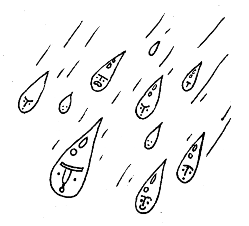
\includegraphics[scale=0.5]{16}}
\end{figure}
\end{SBSection*}
\end{song}

%\twocolumn
\begin{song}{Двадцать дней}{}{Сказка}{Сказка}{}{}


Двадцать дн\Ch{Dm}{ей} – это смена без дня.\par
“Маловато”,– вам скажут друзь\Ch{Gm}{я,}\par
А вожатый отв\Ch{C}{ет}ит люб\Ch{F}{ой}:\par
Это ср\Ch{Gm}{ок} очень д\Ch{A}{аж}е больш\Ch{Dm}{ой!}\\
 

Припев:\par
\ttМожно з\Ch{Gm C}{а-а-а-а} него усп\Ch{Dm}{ет}ь,\par
\ttНаприм\Ch{Gm}{ер,} полмилли\Ch{A}{он}а песен сп\Ch{Dm}{еть,}\par
\ttНо не к\Ch{Gm}{ажд}ый ведь поймет,\par
\ttКак так быстро раскрыв\Ch{A}{ат}ься может р\Ch{Dm}{от!}\\


Для полярника это не срок:\par
Не успеет просохнуть носок.\par
А вожатый успеет подряд \par
Вымыть, высушить сотню ребят!\\

Припев:\par
\ttВедь за смену, как за год \par
\ttСтолько разных мелочей произойдет,\par
\ttНо пока что нам везет,\par
\ttНас начальство для чего-то бережёт.\\


\newpage
Хоть и длинными кажутся дни,\par
Но как миг пролетели они.\par
Будешь долго потом вспоминать,\par
Как в отбой ты любил слово «СПАААТЬ!!!»\\

Припев:\par
\tt          	— Говорят за двадцать дней \par
\tt          	Все узнаешь о напарнице своей…\par
\tt          	— Только это ерунда,\par
\tt          	Обо всем ты не узнаешь никогда!\\

Смена вряд ли даст ответ:\par
Ты нашел свое призванье или нет.\par
Так что надо продолжать,\par
Двадцать раз по двадцать суток отсчитать!\\

\begin{SBSection*}
\begin{figure}[b!]
\center{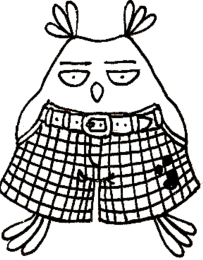
\includegraphics[scale=0.5]{17}}
\end{figure}
\end{SBSection*}

\end{song}

%\twocolumn
\begin{song}{Непогода}{}{Павел Смеян}{Павел Смеян}{}{}

\Ch{D}{Из}менения в природе \Ch{G}{пр}оисходят г\Ch{A}{од} от года,\par
\Ch{D}{Не}погода нынче в моде,\Ch{G}{} н\Ch{F#7}{епог}ода, непогода,\par
\Ch{}Hm{Слов}но из вод\Ch{F#7}{опро}вода \Ch{D7}{ль}ёт на нас с неб\Ch{G}{ес} во\Ch{Hm}{да…}\par
Полг\Ch{G}{од}а плох\Ch{A}{ая} пог\Ch{D}{од}а, \Ch{Hm}{пол}го\Ch{G}{да} — совс\Ch{A}{ем} нику\Ch{D}{да}.\par
Полг\Ch{G}{од}а плох\Ch{A}{ая} пог\Ch{D}{од}а, \Ch{Hm}{пол}го\Ch{G}{да} — сов\Ch{F#7}{сем} нику\Ch{Hm}{да.}\\


\SBChorusTagg:\par
\ttНикуда, нику\Ch{Em}{да н}ельз\Ch{A}{я} укр\Ch{D}{ы}ться н\Ch{Hm}{ам,}\par
\ttНо откладывать ж\Ch{Em}{изнь} ни\Ch{A}{как} нель\Ch{D}{зя}, \Ch{Hm}{}\par
\ttНикуда, нику\Ch{Em}{да, н}о зн\Ch{A}{ай}, что гд\Ch{D}{е}-то т\Ch{Hm}{ам}\par
\ttКто-то ищет теб\Ch{G}{я} сре\Ch{F#7}{ди д}ожд\Ch{Hm}{я.} \Ch{A}{}\\


Грома грозные раскаты от заката до восхода,\par
За грехи людские плата — непогода, непогода,\par
Не ангина, не простуда, посерьёзнее беда.\par
Полгода плохая погода, полгода — совсем никуда\par,
Полгода плохая погода, полгода — совсем никуда.\\\


\SBChorusTagg:\par
\ttНикуда, нику\Ch{Em}{да н}ельз\Ch{A}{я} укр\Ch{D}{ы}ться н\Ch{Hm}{ам,}\par
\ttНо откладывать ж\Ch{Em}{изнь} ни\Ch{A}{как} нель\Ch{D}{зя}, \Ch{Hm}{}\par
\ttНикуда, нику\Ch{Em}{да, н}о зн\Ch{A}{ай}, что гд\Ch{D}{е}-то т\Ch{Hm}{ам}\par
\ttКто-то ищет теб\Ch{G}{я} сре\Ch{F#7}{ди д}ожд\Ch{Hm}{я.} \Ch{A}{}\\


\end{song}

%\twocolumn
\begin{song}{Птенцы}{}{Сказка}{Сказка}{}{}

\Ch{Am}{}  \Ch{Am}{}

Как птенцы из гнез\Ch{Dm}{да} мы \Ch{E}{вы}па\Ch{Am}{ли.}\par
Ты не бойся при\Ch{Dm}{хо}да \Ch{G}{ве}че\Ch{C}{ра.}\par
Под та\Ch{A7}{ки}ми боль\Ch{F}{ши}ми \Ch{A7}{ли}па\Ch{Dm}{ми}\par
Нам с то\Ch{F}{бой} опа\Ch{Dm}{сать}ся \Ch{F}{не}\Ch{E}{че}\Ch{Am}{го.}\\
 
Под такими густыми звёздами -\par
Разве их не для нас рассыпали,\par
Мы не против гнездовья - просто мы\par
Из него ненароком выпали.\\

Это только вначале кажется,\par
Что без дома прожить нельзя никак,\par
Что важней пропитанья кашица,\par
Чем огромные звёзды на небе.\\

Ты не бойся ни тьмы, ни холода.\par
Будет день и найдётся пища нам,\par
Мы ещё пролетим над городом\par
На крыле до небес возвышенном.\\

Пролетим ещё - эка невидаль\par
Над Нью-Йорком, Парижем, Триполи\par
И над липой, откуда некогда,\par
Как птенцы из гнезда мы выпали.\\

Как птенцы из гнезда мы выпали.\par
Ты не бойся прихода вечера.\par
Под такими большими липами\par
Нам с тобой опасаться нечего.\\

\end{song}

%\twocolumn
\begin{song}{Продавец зонтиков}{}{Веня Дркин}{Веня Дркин}{}{}

\Ch{Am}{Город} этот выдумал о\Ch{Dm}{дин} художник,\par
\Ch{G}{Лю}ди в нем не знали, что та\Ch{C}{ко}е дождик.\par
\Ch{A7}{Про}сто не слыхали, что та\Ch{Dm}{ко}е зонтик –\par
\Ch{E7}{Вот} такие люди жили в \Ch{Am}{го}роде том.\par
И один чудак, в старый плащ одетый,\par
Продавал там зонтики зимой и летом,\par
Продавал там зонтики зимой и летом\par
И такую песенку он напевал:\\

\SBChorusTagg:\par
\tt“Господа, купите зонтик.\par
\ttБелый зонтик, красный зонтик,\par
\ttЖелтый зонтик, синий зонтик –\par
\ttМожет пригодится вам.”\\

Были домики у них из пластилина,\par
Из пустых коробочек автомашины,\par
И, не опасаясь никакой ангины,\par
Маленькие люди жили в городе том.\par
Маленькие были у людей заботы:\par
Шли они в кино или в театр с работы.\par
Вечером в подъезде целовался кто-то.\par
Все шутили и смеялись над стариком.\\


\SBChorusTagg.\\

\newpage

Маленькое небо как-то вдруг намокло,\par
В крошечных домишках задрожали стекла,\par
И огромный дождь пошел гулять по крышам,\par
Сразу все схватили насморк в городе том.\par
Вспомнили тут люди о торговце старом,\par
Кинулись искать его по всем базарам,\par
Но исчез торговец со своим товаром.\par
Только песенка осталась в память о нем:\\

\SBChorusTagg.\par

\begin{SBSection*}
\begin{figure}[b!]
\center{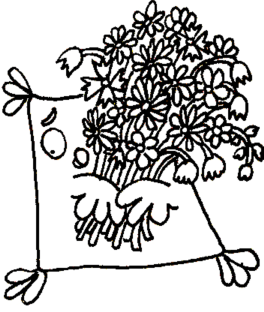
\includegraphics[scale=0.5]{15}}
\end{figure}
\end{SBSection*}

\end{song}

%\twocolumn
\begin{song}{Белая гвардия}{}{Белая гвардия}{Белая гвардия}{}{}

Проигрыш: (2 раза)\par 
\Ch{Am}{} \Ch{D}{} \Ch{G}{} \Ch{C}{} \Ch{Am}{} \Ch{H7}{} \Ch{Em}\\

\Ch{Em}{Белая} гвардия, белый снег,\par
\Ch{Am7}{Белая} музыка революций.\par
\Ch{D7}{Белая} женщина, нервный смех,\par
\Ch{G}{Белого} платья слегка коснуться.\par
 
Белой рукой распахнуть окно,\par
Белого света в нем не видя.\par
Белое выпить до дна вино,\par
В красную улицу в белом выйти.\\

Припев:\par
\ttКог\Ch{Em}{да} ты вернешься,\par
\ttВсе будет и\Ch{Am}{на}че, и нам бы узнать друг друга,\par
\ttКог\Ch{D7}{да} ты вернешься,\par
\ttА я не же\Ch{G}{на} и даже \Ch{H7}{не} подруга.\par
\ttКог\Ch{C}{да} ты вернешься,\par
\ttКо мне, так без\Ch{Am}{ум}но тебя любившей в прошлом,\par
\tt\Ch{D7}{Ко}гда ты вернешься -\par
\ttУвидишь, что ж\Ch{G}{ре}бий давно и не \Ch{E7}{нами} брошен.\\

Проигрыш.\\
 
\newpage
Сизые сумерки прошлых лет\par
Робко крадутся по переулкам.\par
В этом окне еле брезжит свет,\par
Ноты истрепаны, звуки гулки.\par
Тонкие пальцы срывают аккорд...\par
Нам не простят безрассудного дара.\par
Бьются в решетку стальных ворот\par
Пять океанов земного шара.\\

Припев. \par
Проигрыш.\\
 
Красный трамвай простучал в ночи,\par
Красный закат догорел в бокале,\par
Красные-красные кумачи\par
С красных деревьев на землю упали.\par
Я не ждала тебя в октябре,\par
Виделись сны, я листала сонник:\par
Красные лошади на заре\par
Били копытами о подоконник.\\

Припев:\par
\ttКогда ты вернешься,\par
\ttВсе будет иначе, и нам бы узнать друг друга,\par
\ttКогда ты вернешься,\par
\ttА я не жена и даже не подруга.\par
\ttКогда ты вернешься,\par
\ttВернешься в наш город обетованный,\par
\ttКогда ты вернешься -\par
\ttТакой невозможный и такой желанный?\\

Проигрыш.\par

\end{song}

%\twocolumn
\begin{song}{Перевал}{}{Песни у костра}{Песни у костра}{}{}


\Ch{Am}{Про}сто нечего нам \Ch{Dm}{боль}ше терять\par
\Ch{E}{Всё} нам вспомнится на \Ch{Am}{Страшном} суде.\par
Эта ночь легла, как \Ch{Dm}{тот} перевал,\par
\Ch{G}{За} которым испол\Ch{C}{нень}е надежд.\par
\Ch{A7}{Про}сто прожитое—про\Ch{Dm}{жи}то зря, \Ch{G}{}\par
Но не в этом, пони\Ch{C}{мае}шь ли, соль… \Ch{Am}{}\par
Слышишь, падают дож\Ch{Dm}{ди} октября.\par
\Ch{E}{Ви}дишь, старый дом сто\Ch{Am}{ит} средь лесов.\\

Мы затопим в доме печь, в доме печь,\par
Мы гитару позовем со стены.\par
Просто нечего нам больше беречь,\par
Ведь за нами все мосты сожжены.\par
Все мосты, все перекрёстки дорог,\par
Все прошёптанные тайны в ночи.\par
Каждый сделал все, что смог, все, что смог,\par
Мы об этом помолчим, помолчим.\\


И луна взойдет заплывшей свечой,\par
Ставни скрипнут  на ветру, на ветру.\par
Ах, как я тебя люблю горячо,\par
Это годы не сотрут, не сотрут.\par
Мы оставшихся друзей соберем,\par
Мы набьем картошкой старый рюкзак,\par
Люди спросят: "Что за шум, что за гам?"\par
Мы ответим: "Просто так,  просто так”...\\

\newpage

    Просто так идут дожди в октябре,\par
    И потеряны от счастья ключи.\par
    Это всё, конечно, мне, конечно, мне,\par
    Но об этом помолчим, помолчим.\par
    Просто прожитое—прожито зря,\par
    Но не в этом, понимаешь ли, соль…\par
    Слышишь, падают дожди октября.\par
    Видишь, старый дом стоит средь лесов.\par


\begin{SBSection*}
\begin{figure}[b!]
\center{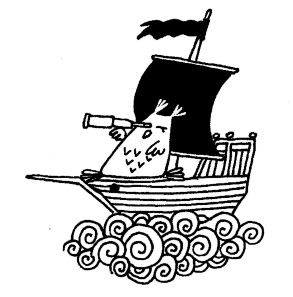
\includegraphics[scale=0.5]{22}}
\end{figure}
\end{SBSection*}

\end{song}

%\twocolumn
\begin{song}{Ленинградская (Все расстояния)}{}{Песни у костра}{Песни у костра}{}{}

\Ch{Am}{Все} расстоянья когда-нибудь в круг замы\Ch{E}{ка}ются,\par
\Ch{E}{Все} из разлук обязательно \Ch{E7}{встре}чей кон\Ch{Am}{ча}ются;\par
Должны про\Ch{Dm}{плыть} вокруг Зем\Ch{G}{ли,}\par
Вернуться в \Ch{C}{га}вань кораб\Ch{F}{ли,}\par   
Все поез\Ch{Dm}{да} в свои вер\Ch{E}{нуть}ся горо\Ch{Am}{да.}\\
 
Шумный вокзал то встречает друзей , то прощается,\par
Мы расстаемся, но снова назад возвращаемся -\par
Чтоб снова встать в огромный круг,\par
И снова знать, что рядом друг ,\par
И песни петь, чтоб больше не было разлук.\\
 
Все расстоянья когда-нибудь в круг замыкаются,\par
Все из разлук обязательно встречей кончаются;\par
И через год, и через пять,\par
Мы с вами встретимся опять,\par
Ничто не сможет нашей дружбе помешать.\par

\end{song}

%\twocolumn
\begin{song}{Десять капель}{}{Танцы Минус}{Танцы Минус}{}{}

Проигрыш: (2 раза)\par 
\Ch{C}{} \Ch{E}{} \Ch{Am}{} \Ch{F}{} \Ch{C}{} \Ch{E}{} \Ch{Am}{} \Ch{F}{}

\Ch{C}{Де}сять капель дож\Ch{E}{дя} у тебя на пле\Ch{Am}{че}\par
Ты забыла свой \Ch{F}{зонт,} ты спешила ко \Ch{C}{мне.}\par
Десять капель дож\Ch{E}{дя} на плече у те\Ch{Am}{бя,}\par
Десять капель люб\Ch{F}{ви,} десять капель ог\Ch{C}{ня}\\

Припев:\\(Три первых слова в припеве дублируются вторым голосом)\par
\tt\Ch{C}{Т}воя\Ch{E}{} ладо\Ch{Am}{нь} горит\Ch{F}{} в моих руках\par
\tt\Ch{C}{Л}юбви\Ch{E}{ }пож\Ch{Am}{ар} горит в тво\Ch{F}{их} глазах\\

Проигрыш.\\

Время делает шаг, время делает круг\par
Мы забудем друзей, мы забудем подруг\par
Просто выпьем вина из любви и огня\par
Десять капель меня, десять капель тебя\\

Припев.\\

Голос твой в тишине околдует меня\par
Ярким жарким огнем стану я до утра\par
Ты прикажешь гори, и я вспыхну любя\par
В этом пламени ты, в этом пламени я.\par

\end{song}

%\twocolumn
\begin{song}{Макет}{}{Песни у костра}{Сказка}{}{}
sadfsfthanks,\par
\begin{SBOpGroup}
asdas\
\end{SBOpGroup}
\begin{SBSection*}fdf\end{SBSection*}
\begin{SBVerse*}\end{SBVerse*}
\begin{SBChorus*}\end{SBChorus*}

\begin{SBOccurs}{23}
dsf
\end{SBOccurs}

\begin{SBSection*}
\begin{figure}[b!]
\center{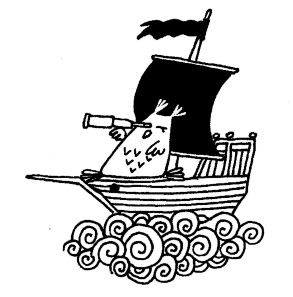
\includegraphics[scale=0.5]{22}}
\end{figure}
\end{SBSection*}
\end{song}

\mainmatter

\renewcommand{\footrulewidth}{0.0pt}
\renewcommand{\item}{\par\hangindent=40pt}
\renewcommand{\subitem}{\par\hangindent=40pt \hspace*{20pt}}
\renewcommand{\subsubitem}{\par\hangindent=40pt \hspace*{30pt}}

\newpage
\raggedright%\documentclass[a5paper,11pt]{book}
%\usepackage{fancyhdr}
%\usepackage[chordbk]{songbook}
%
%\usepackage[T2A]{fontenc}
%\usepackage[utf8]{inputenc}
%\usepackage[russian]{babel}
%
%\title{A Church Songbook}
%\author{}
%\date{Revised:  \RevDate}
%
%\newcommand{\RelDate}{13 November'19}
%\newcommand{\RevDate}{\today}

\documentclass[11pt,a5paper]{book}
\usepackage[a5paper]{geometry}
\usepackage[chordbk]{songbook}
\usepackage[T2A]{fontenc}
\usepackage[utf8]{inputenc}
\usepackage[russian]{babel}
\usepackage{cmap} % для работы поиска кириллицы в pdf

%\usepackage{amsmath,amsthm,amssymb}
%\usepackage{mathtext}


\usepackage[pdftex]{graphicx}
\usepackage{lscape}
%\usepackage{vmargin}
\usepackage{textcomp}
\usepackage{setspace}
%\usepackage{marvosym}
\usepackage{gensymb} %%%for \micro tag
\usepackage{upgreek} %%% \upmu
\usepackage{tipa}
\usepackage{phonetic}
%\usepackage[greek,english]{babel}
\usepackage{threeparttable}
\usepackage{multirow}
\usepackage{harvard}
\usepackage{longtable}
\renewcommand{\sectionmark}[1]{\markright{#1}}
\renewcommand{\chaptermark}[1]{\markboth{#1}{}}
\addto\captionsenglish{\renewcommand{\bibname}{References}}
\usepackage{latexsym,fancyhdr}

\newcommand{\RelDate}{26 Апреля'1984}
\newcommand{\RevDate}{\today}

%%%
% C.C.L.I. license number definition; for copyright licensing info.
% One of these macros will be manually inserted into the {CpyRt}
% parameter of the {song} environment.
%
%       \CCLInumber - The actual copyright license number.  Don't
%               insert this command in the {CpyRt} parameter, use one
%               of the others.
%       \CCLIed - Indicates a song falls under our CCLI license.
%       \NotCCLIed - Indicates a song doesn't fall under our CCLI
%               license.  Public Domain songs fall into this category.
%       \PGranted - We have received specific permission from the
%               copyright holder to use this song.
%       \PPending - We are in the process of obtaining permission to
%               use this song.
%%%
\newcommand{\CCLInumber}{Your CCLI Number}
\newcommand{\CCLIed}{{\CpyRtInfoFont (CCLI \CCLInumber)}}
\newcommand{\NotCCLIed}{\relax}
\newcommand{\PGranted}{\relax}
\newcommand{\PPending}{{\CpyRtInfoFont (Permission Pending)}}

%%%
% Title page information.
%%%
\title{ Сказочный песенник}
\author{}
\date{Созданно:  \RevDate}


%%%
% Define fonts to use in the headers and footers of the songbook.
%%%
\newcommand{\LHeadFont}{\normalsize}            % = cmr12  at 12pt
\newcommand{\CHeadFont}{\normalsize\rm}         % = cmr12  at 12pt
\newcommand{\RHeadFont}{\normalsize}            % = cmr12  at 12pt
\newcommand{\LFootFont}{\scriptsize}            % = cmr8   at  8pt
\newcommand{\CFootFont}{\tiny\myTinySF}         % = cmss8  at  8pt
\newcommand{\RFootFont}{\scriptsize}            % = cmr8   at  8pt

%%%
% Turn on and define fancy page heading/footing definition.
%%%
\pagestyle{fancy}

\ifChordBk
  % It's a words & chords songbook...
%  \addtolength{\headwidth}{\marginparsep}
%  \addtolength{\headwidth}{\marginparwidth}
  \renewcommand{\headrulewidth}{0.0pt}
  \renewcommand{\footrulewidth}{0.0pt}
%  \fancyhead[LE,RO]{\LHeadFont\emph{\leftmark\/}}
%  \fancyhead[CE,CO]{\CHeadFont\thepage}
  \fancyhead[RE,LO]{~}
\else\ifOverhead
  % It's an overhead...
  \renewcommand{\footrulewidth}{0pt}
  \renewcommand{\headrulewidth}{0pt}
  \fancyhead[LE,RO]{}
  \fancyhead[CE,CO]{}
  \fancyhead[RE,LO]{}
\else\ifWordBk
  % It's a words only songbook...
  \addtolength{\headwidth}{\marginparsep}
  \addtolength{\headwidth}{\marginparwidth}
  \renewcommand{\headrulewidth}{0.0pt}
  \renewcommand{\footrulewidth}{0.0pt}
  \fancyhead[LE,RO]{\LHeadFont A Church Songbook}
  \fancyhead[CE,CO]{\CHeadFont\thepage}
  \fancyhead[RE,LO]{\RHeadFont\RelDate}
\fi\fi\fi

%\fancyfoot[LE,RO]{\LFootFont Property of The Church}
%\ifSongEject
%  \fancyfoot[CE,CO]{\CFootFont \RevDate}
%\else
%  \fancyfoot[CE,CO]{\CFootFont}
%\fi
%\fancyfoot[RE,LO]{\RFootFont Material used by permission.}

%%%
% Turn on/off index-file generation.  Uncomment the \makeindex line to
% turn index generation on;  comment it out to turn index generation
% off.
%%%
\makeTitleIndex         %% Title and First Line Index.
\makeTitleContents      %% Table of Contents.
\makeKeyIndex           %% Index of song by key.
\graphicspath{{img/}} % папка с картинками
\DeclareGraphicsExtensions{.pdf,.png,.jpg} % форматы, которые будем считать картинками

%\newenvironment{song}[7][Y]{
%% Comment markers to negate
%\if#1Y\ExcludeSongfalse\else\ExcludeSongtrue\fi% the newline.
%\ifPrintAllSongs\ExcludeSongfalse\fi
%\SongMarkboth{\relax}{\relax}
%\SBinSongEnvtrue
%\renewcommand{\SBinSongEnv}{\True}
%\ifWordsOnly
%	\setlength{\parindent}{0pt}
%\fi

%%%
% Redefine fonts from SongBook style that I don't like.
%%%
\font\myTinySF=cmss8 at 8pt
\renewcommand{\CpyRtInfoFont}{\tiny\myTinySF}


%
%\font\myTinySF=cmss8    at  8pt
%\font\myHugeSF=cmssbx10 at 25pt
%\renewcommand{\CpyRtInfoFont}{\tiny\myTinySF}
%\newcommand{\myTitleFont}{\Huge\myHugeSF}
%\newcommand{\mySubTitleFont}{\large\sf}

%%% Работа с русским языком
%\usepackage[no-math]{fontspec}      %% подготавливает загрузку шрифтов Open Type, True Type и др.
%\defaultfontfeatures{Ligatures={TeX},Renderer=Basic}  %% свойства шрифтов по умолчанию
%\setmainfont[Ligatures={TeX,Historic}]{Times New Roman} %% задаёт основной шрифт документа
%\setsansfont{Helvetica Neue}                    %% задаёт шрифт без засечек

%\newfontfamily{\allods}{AllodsWest}

\newcommand{\SBPubDomm}{~}
\renewcommand{\CpyRt}[3][Y]{%
\if#1Y\begin{center}\fi
\if\blank{#2}%
\if\blank{#3}%
{\CpyRtFont\copyright \SBUnknownTag{} \CpyRtInfoFont}%
\else
{\CpyRtFont\copyright \SBUnknownTag{} \CpyRtInfoFont #3}%
\fi%
\else%
\ifthenelse{\equal{#2}{\SBPubDomm}}
{%then
{\CpyRtFont #2 \CpyRtInfoFont #3}%
}{%else
{\CpyRtFont #2 \CpyRtInfoFont #3}%
}%fi
\fi%
\if#1Y\end{center}\fi
}


\newcommand{\SBUnknownTagg}{~}
\renewcommand{\WAndM}[2][Y]{~}
\renewcommand{\WAndM}[2][Y]{%
\if#1Y\begin{center}\fi
\if\blank{#2}%
{\SBUnknownTagg}%
\else
{~}%
\fi
\if#1Y\end{center}\fi
}

\renewcommand{\STitle}[3][Y]{%
\setcounter{SBVerseCnt}{0}%
\setcounter{SBSectionCnt}{0}%
\ifExcludeSong\relax%
	\else\keyIndex{{\protect\sbChord#3\protect\relax} -- #2}{\theSBSongCnt}\fi%
	\vspace{\SpaceAboveSTitle}%
\if#1Y\begin{center}\fi
	{}{\STitleFont\LARGE #2}%
	\ifWordsOnly\relax\else\fi%
	\if#1Y\end{center}\fi
\STitleMarkboth{#2}{\relax}%
}


%\renewenvironment{SBOpGroup}{%
%	\sbSetsbBaselineSkipAmt%
%	\bgroup%
%	\begin{list}{\hbox{}}
%	  {\setlength {\leftmargin}
%		{\HangAmt}
%		\setlength{\itemindent}
%			{-\HangAmt}
%		\setlength{\listparindent}{-\HangAmt}
%		\setlength{\topsep}{0pt}
%		\setlength{\parsep}{0pt}
%		\setlength{\labelwidth}{0pt}
%		\setlength{\labelsep}{0pt}
%		\setlength{\baselineskip} {\sbBaselineSkipAmt}
%	}%\item}
%{\end{list}%
\newcommand{\SBChorusTagg}{Припев}
\renewenvironment{SBChorus}{%
\sbSetsbBaselineSkipAmt%
\bgroup%
\SBChorusMarkright{\SBChorusTag}
\begin{list}{{\SBChorusTagFont\SBChorusTagg}}
{\setlength {\leftmargin}
{\LeftMarginSBChorus + \HangAmt}
\setlength{\itemindent}
{-\HangAmt}
\setlength{\listparindent}{-\HangAmt}
\setlength{\parsep}
{0pt}
\setlength{\baselineskip} {\sbBaselineSkipAmt}
}%
\item}
{\end{list}%
\egroup%
\SpaceAfterChorus%
}

\renewcommand{\tt}{\indent \indent}
%\renewcommand{\nt}{\noindent}


\usepackage{amsmath}

\makeArtistIndex
\makeTitleIndex         %% Title and First Line Index.
\makeTitleContents      %% Table of Contents.
\makeKeyIndex           %% Index of song by key.
%\usepackage{printallsongs}

\begin{document} 
\maketitle

\mainmatter


\begin{song}{Вожатский гимн}{}{Сказка}{Сказка}{}{}

По \Ch{Am}{ла}герю подъём, нас горн зовёт!\par
Забудь о том, что ночь была бес\Ch{C}{сон}ною\par
Смо\Ch{Dm}{чи} водою \Ch{G}{ве}ки воспа\Ch{C}{лён}\Ch{F}{ные}\par    
По\Ch{Dm}{вя}зывай свой \Ch{E}{галс}тук — и впе\Ch{Am (A7)}{рёд!}\par
Смо\Ch{Dm}{чи} водою \Ch{G}{ве}ки воспа\Ch{C}{лён}\Ch{F}{ные}\par    
По\Ch{Dm}{вя}зывай свой \Ch{E}{галс}тук — и впе\Ch{Am (A7)}{рёд!}\par

%	\begin{SBChorus*}
\ttНе\Ch{E}{про}сто воспитывать \Ch{Am}{но}вых людей,\par
\ttНу \Ch{E}{что} ж, это наша с то\Ch{Am}{бою} свя\Ch{A7}{ты}ня.\par
\ttМой \Ch{Dm}{друг}, нам до\Ch{G}{ве}рили \Ch{C}{ду}ши де\Ch{F}{тей},\par
\ttИх \Ch{Dm}{ра}достный \Ch{Am}{смех} нам на\Ch{E}{гра}да от\Ch{Am}{ны}не.\par
\ttМой \Ch{Dm}{друг}, нам до\Ch{G}{ве}рили \Ch{C}{ду}ши де\Ch{F}{тей},\par
\ttИх \Ch{Dm}{ра}достный \Ch{Am}{смех} нам на\Ch{E}{гра}да от\Ch{Am}{ны}не.\\
%\end{SBChorus*}

Отбой, засыпает детвора.\par
Взгляни на их улыбки полусонные,\par
Пускай им снятся острова зелёные,\par
А нам опять работать до утра!\par
Пускай им снятся острова зелёные,\par
А нам опять работать до утра!\par

\tt И пусть от бессилья затихнешь не раз,\par
\ttИ голос усталый до хрипа натружен,\par
\ttПусть будут умней и счастливее нас\par
\ttТе дети, в которых вложили мы души!\par
\ttПусть будут умней и счастливее нас\par
\ttТе дети, в которых вложили мы души!

\end{song}

\begin{song}{Сказка в неглиже}{}{Сказка}{Сказка}{}{}

Есть у \Ch{C}{каж}дого добрая сказка в ду\Ch{F}{ше,}\par 
Надо \Ch{G}{толь}ко прочесть этой сказки стра\Ch{C}{ни}цы.\par
В тиши\Ch{C}{не}, разо\Ch{C7}{де}тая вся в негли\Ch{F}{же,}\par
Пусть на\Ch{G}{ве}ки она, пусть на\Ch{F}{ве}ки она сохра\Ch{C}{ни}тся. \Ch{C7}{ }\par 
В тиши\Ch{F}{не,} разо\Ch{G}{де}тая вся в негли\Ch{C}{же,} \Ch{Am}{}\par
Пусть на\Ch{F}{ве}ки она, пусть на\Ch{G}{ве}ки она сохра\Ch{C}{ни}тся.\\


\ttЭту сказку пред другом раскрыть поспеши,\par
\ttА врагу не спеши эту сказку поведать.\par
\ttПусть растут и читают ее малыши.\par
\ttБудь добрей, и тебя минут всякие беды.\par
\ttПусть растут и читают ее малыши.\par
\ttБудь добрей, и тебя минут всякие беды.\\


\Ch{C7}{}Будет \Ch{F}{мно}го распутий, \Ch{G}{до}рог и тре\Ch{C}{вог.}\Ch{Am}{}\par
На вис\Ch{F}{ки} твои ляжет \Ch{G}{не}тающий \Ch{C}{ин}ей, \Ch{C7}{}\par
И пой\Ch{F}{мёшь,} научившись чи\Ch{G}{тать} между \Ch{C}{строк:} \Ch{Am}{}\par
Даже \Ch{F}{гнус}ный злодей \Ch{G}{в} этой сказке не\Ch{C}{ви}нен. \Ch{C7}{}\par
И пой\Ch{F}{мёшь,} научившись чи\Ch{G}{тать} между ст\Ch{C}{рок:} \Ch{A}{}\par
Даже \Ch{F}{гнус}ный злодей \Ch{G}{в} этой сказке не\Ch{C}{ви}нен.\\

\Ch{C}{} \Ch{G}{} \Ch{F}{} \Ch{G}{} \Ch{C}{} \Ch{C7}{}\par
\Ch{C}{} \Ch{G}{} \Ch{F}{} \Ch{G}{} \Ch{C}{}
\end{song}

%\twocolumn
\begin{song}{Вожатский марш}{}{Сказка}{Сказка}{}{}

Есть на\Ch{Am}{род} у нас весёлый,\par
Самой \Ch{C}{луч}шей в мире пробы,\par
Песни \Ch{G}{петь} всегда мас\Ch{C}{так.}\Ch{A7}{}\par
Он всег\Ch{Dm}{да} всего добьётся,\par
Он Вожа\Ch{Am}{ты}ми зовётся,\par
\Ch{E}{Так} и только \Ch{Am (A7)}{так!}\par
Он всег\Ch{Dm}{да} всего добьётся,\par
Он Во\Ch{Am}{жа}тыми зовётся,\par
\Ch{E}{Так} и только \Ch{Am (A7)}{так!}\\

Домосед привязан к дому\par
И по случаю такому,\par
Он из дома — ни на шаг!\par
А вожатый — он в дороге,\par
Он готов в огонь и в воду,\par
Так и только так!\par
А вожатый — он в дороге,\par
Он готов в огонь и в воду,\par
Так и только так!\\
\newpage
Жадный денежки считает,\par
Все считает и считает,\par
К пятаку кладет пятак.\par
А вожатый деньги тратит,\par
Не боясь, что их не хватит,\par
Так и только так!\par
А вожатый деньги тратит,\par
Не боясь, что их не хватит,\par
Так и только так!\\

Холостяк в любовь не верит,\par
Все не верит и не верит,\par
Потому что холостяк.\par
А вожатых не влюблённых\par
Не найдёшь определённо,\par
Так и только так!\par
А вожатых не влюблённых\par
Не найдёшь определённо,\par
Так и только так!\par

\begin{SBSection*}
\begin{figure}[b!]
\center{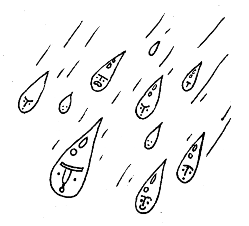
\includegraphics[scale=0.5]{16}}
\end{figure}
\end{SBSection*}
\end{song}

%\twocolumn
\begin{song}{Двадцать дней}{}{Сказка}{Сказка}{}{}


Двадцать дн\Ch{Dm}{ей} – это смена без дня.\par
“Маловато”,– вам скажут друзь\Ch{Gm}{я,}\par
А вожатый отв\Ch{C}{ет}ит люб\Ch{F}{ой}:\par
Это ср\Ch{Gm}{ок} очень д\Ch{A}{аж}е больш\Ch{Dm}{ой!}\\
 

Припев:\par
\ttМожно з\Ch{Gm C}{а-а-а-а} него усп\Ch{Dm}{ет}ь,\par
\ttНаприм\Ch{Gm}{ер,} полмилли\Ch{A}{он}а песен сп\Ch{Dm}{еть,}\par
\ttНо не к\Ch{Gm}{ажд}ый ведь поймет,\par
\ttКак так быстро раскрыв\Ch{A}{ат}ься может р\Ch{Dm}{от!}\\


Для полярника это не срок:\par
Не успеет просохнуть носок.\par
А вожатый успеет подряд \par
Вымыть, высушить сотню ребят!\\

Припев:\par
\ttВедь за смену, как за год \par
\ttСтолько разных мелочей произойдет,\par
\ttНо пока что нам везет,\par
\ttНас начальство для чего-то бережёт.\\


\newpage
Хоть и длинными кажутся дни,\par
Но как миг пролетели они.\par
Будешь долго потом вспоминать,\par
Как в отбой ты любил слово «СПАААТЬ!!!»\\

Припев:\par
\tt          	— Говорят за двадцать дней \par
\tt          	Все узнаешь о напарнице своей…\par
\tt          	— Только это ерунда,\par
\tt          	Обо всем ты не узнаешь никогда!\\

Смена вряд ли даст ответ:\par
Ты нашел свое призванье или нет.\par
Так что надо продолжать,\par
Двадцать раз по двадцать суток отсчитать!\\

\begin{SBSection*}
\begin{figure}[b!]
\center{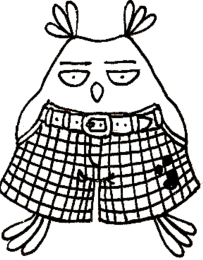
\includegraphics[scale=0.5]{17}}
\end{figure}
\end{SBSection*}

\end{song}

%\twocolumn
\begin{song}{Непогода}{}{Павел Смеян}{Павел Смеян}{}{}

\Ch{D}{Из}менения в природе \Ch{G}{пр}оисходят г\Ch{A}{од} от года,\par
\Ch{D}{Не}погода нынче в моде,\Ch{G}{} н\Ch{F#7}{епог}ода, непогода,\par
\Ch{}Hm{Слов}но из вод\Ch{F#7}{опро}вода \Ch{D7}{ль}ёт на нас с неб\Ch{G}{ес} во\Ch{Hm}{да…}\par
Полг\Ch{G}{од}а плох\Ch{A}{ая} пог\Ch{D}{од}а, \Ch{Hm}{пол}го\Ch{G}{да} — совс\Ch{A}{ем} нику\Ch{D}{да}.\par
Полг\Ch{G}{од}а плох\Ch{A}{ая} пог\Ch{D}{од}а, \Ch{Hm}{пол}го\Ch{G}{да} — сов\Ch{F#7}{сем} нику\Ch{Hm}{да.}\\


\SBChorusTagg:\par
\ttНикуда, нику\Ch{Em}{да н}ельз\Ch{A}{я} укр\Ch{D}{ы}ться н\Ch{Hm}{ам,}\par
\ttНо откладывать ж\Ch{Em}{изнь} ни\Ch{A}{как} нель\Ch{D}{зя}, \Ch{Hm}{}\par
\ttНикуда, нику\Ch{Em}{да, н}о зн\Ch{A}{ай}, что гд\Ch{D}{е}-то т\Ch{Hm}{ам}\par
\ttКто-то ищет теб\Ch{G}{я} сре\Ch{F#7}{ди д}ожд\Ch{Hm}{я.} \Ch{A}{}\\


Грома грозные раскаты от заката до восхода,\par
За грехи людские плата — непогода, непогода,\par
Не ангина, не простуда, посерьёзнее беда.\par
Полгода плохая погода, полгода — совсем никуда\par,
Полгода плохая погода, полгода — совсем никуда.\\\


\SBChorusTagg:\par
\ttНикуда, нику\Ch{Em}{да н}ельз\Ch{A}{я} укр\Ch{D}{ы}ться н\Ch{Hm}{ам,}\par
\ttНо откладывать ж\Ch{Em}{изнь} ни\Ch{A}{как} нель\Ch{D}{зя}, \Ch{Hm}{}\par
\ttНикуда, нику\Ch{Em}{да, н}о зн\Ch{A}{ай}, что гд\Ch{D}{е}-то т\Ch{Hm}{ам}\par
\ttКто-то ищет теб\Ch{G}{я} сре\Ch{F#7}{ди д}ожд\Ch{Hm}{я.} \Ch{A}{}\\


\end{song}

%\twocolumn
\begin{song}{Птенцы}{}{Сказка}{Сказка}{}{}

\Ch{Am}{}  \Ch{Am}{}

Как птенцы из гнез\Ch{Dm}{да} мы \Ch{E}{вы}па\Ch{Am}{ли.}\par
Ты не бойся при\Ch{Dm}{хо}да \Ch{G}{ве}че\Ch{C}{ра.}\par
Под та\Ch{A7}{ки}ми боль\Ch{F}{ши}ми \Ch{A7}{ли}па\Ch{Dm}{ми}\par
Нам с то\Ch{F}{бой} опа\Ch{Dm}{сать}ся \Ch{F}{не}\Ch{E}{че}\Ch{Am}{го.}\\
 
Под такими густыми звёздами -\par
Разве их не для нас рассыпали,\par
Мы не против гнездовья - просто мы\par
Из него ненароком выпали.\\

Это только вначале кажется,\par
Что без дома прожить нельзя никак,\par
Что важней пропитанья кашица,\par
Чем огромные звёзды на небе.\\

Ты не бойся ни тьмы, ни холода.\par
Будет день и найдётся пища нам,\par
Мы ещё пролетим над городом\par
На крыле до небес возвышенном.\\

Пролетим ещё - эка невидаль\par
Над Нью-Йорком, Парижем, Триполи\par
И над липой, откуда некогда,\par
Как птенцы из гнезда мы выпали.\\

Как птенцы из гнезда мы выпали.\par
Ты не бойся прихода вечера.\par
Под такими большими липами\par
Нам с тобой опасаться нечего.\\

\end{song}

%\twocolumn
\begin{song}{Продавец зонтиков}{}{Веня Дркин}{Веня Дркин}{}{}

\Ch{Am}{Город} этот выдумал о\Ch{Dm}{дин} художник,\par
\Ch{G}{Лю}ди в нем не знали, что та\Ch{C}{ко}е дождик.\par
\Ch{A7}{Про}сто не слыхали, что та\Ch{Dm}{ко}е зонтик –\par
\Ch{E7}{Вот} такие люди жили в \Ch{Am}{го}роде том.\par
И один чудак, в старый плащ одетый,\par
Продавал там зонтики зимой и летом,\par
Продавал там зонтики зимой и летом\par
И такую песенку он напевал:\\

\SBChorusTagg:\par
\tt“Господа, купите зонтик.\par
\ttБелый зонтик, красный зонтик,\par
\ttЖелтый зонтик, синий зонтик –\par
\ttМожет пригодится вам.”\\

Были домики у них из пластилина,\par
Из пустых коробочек автомашины,\par
И, не опасаясь никакой ангины,\par
Маленькие люди жили в городе том.\par
Маленькие были у людей заботы:\par
Шли они в кино или в театр с работы.\par
Вечером в подъезде целовался кто-то.\par
Все шутили и смеялись над стариком.\\


\SBChorusTagg.\\

\newpage

Маленькое небо как-то вдруг намокло,\par
В крошечных домишках задрожали стекла,\par
И огромный дождь пошел гулять по крышам,\par
Сразу все схватили насморк в городе том.\par
Вспомнили тут люди о торговце старом,\par
Кинулись искать его по всем базарам,\par
Но исчез торговец со своим товаром.\par
Только песенка осталась в память о нем:\\

\SBChorusTagg.\par

\begin{SBSection*}
\begin{figure}[b!]
\center{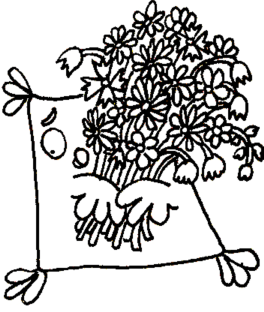
\includegraphics[scale=0.5]{15}}
\end{figure}
\end{SBSection*}

\end{song}

%\twocolumn
\begin{song}{Белая гвардия}{}{Белая гвардия}{Белая гвардия}{}{}

Проигрыш: (2 раза)\par 
\Ch{Am}{} \Ch{D}{} \Ch{G}{} \Ch{C}{} \Ch{Am}{} \Ch{H7}{} \Ch{Em}\\

\Ch{Em}{Белая} гвардия, белый снег,\par
\Ch{Am7}{Белая} музыка революций.\par
\Ch{D7}{Белая} женщина, нервный смех,\par
\Ch{G}{Белого} платья слегка коснуться.\par
 
Белой рукой распахнуть окно,\par
Белого света в нем не видя.\par
Белое выпить до дна вино,\par
В красную улицу в белом выйти.\\

Припев:\par
\ttКог\Ch{Em}{да} ты вернешься,\par
\ttВсе будет и\Ch{Am}{на}че, и нам бы узнать друг друга,\par
\ttКог\Ch{D7}{да} ты вернешься,\par
\ttА я не же\Ch{G}{на} и даже \Ch{H7}{не} подруга.\par
\ttКог\Ch{C}{да} ты вернешься,\par
\ttКо мне, так без\Ch{Am}{ум}но тебя любившей в прошлом,\par
\tt\Ch{D7}{Ко}гда ты вернешься -\par
\ttУвидишь, что ж\Ch{G}{ре}бий давно и не \Ch{E7}{нами} брошен.\\

Проигрыш.\\
 
\newpage
Сизые сумерки прошлых лет\par
Робко крадутся по переулкам.\par
В этом окне еле брезжит свет,\par
Ноты истрепаны, звуки гулки.\par
Тонкие пальцы срывают аккорд...\par
Нам не простят безрассудного дара.\par
Бьются в решетку стальных ворот\par
Пять океанов земного шара.\\

Припев. \par
Проигрыш.\\
 
Красный трамвай простучал в ночи,\par
Красный закат догорел в бокале,\par
Красные-красные кумачи\par
С красных деревьев на землю упали.\par
Я не ждала тебя в октябре,\par
Виделись сны, я листала сонник:\par
Красные лошади на заре\par
Били копытами о подоконник.\\

Припев:\par
\ttКогда ты вернешься,\par
\ttВсе будет иначе, и нам бы узнать друг друга,\par
\ttКогда ты вернешься,\par
\ttА я не жена и даже не подруга.\par
\ttКогда ты вернешься,\par
\ttВернешься в наш город обетованный,\par
\ttКогда ты вернешься -\par
\ttТакой невозможный и такой желанный?\\

Проигрыш.\par

\end{song}

%\twocolumn
\begin{song}{Перевал}{}{Песни у костра}{Песни у костра}{}{}


\Ch{Am}{Про}сто нечего нам \Ch{Dm}{боль}ше терять\par
\Ch{E}{Всё} нам вспомнится на \Ch{Am}{Страшном} суде.\par
Эта ночь легла, как \Ch{Dm}{тот} перевал,\par
\Ch{G}{За} которым испол\Ch{C}{нень}е надежд.\par
\Ch{A7}{Про}сто прожитое—про\Ch{Dm}{жи}то зря, \Ch{G}{}\par
Но не в этом, пони\Ch{C}{мае}шь ли, соль… \Ch{Am}{}\par
Слышишь, падают дож\Ch{Dm}{ди} октября.\par
\Ch{E}{Ви}дишь, старый дом сто\Ch{Am}{ит} средь лесов.\\

Мы затопим в доме печь, в доме печь,\par
Мы гитару позовем со стены.\par
Просто нечего нам больше беречь,\par
Ведь за нами все мосты сожжены.\par
Все мосты, все перекрёстки дорог,\par
Все прошёптанные тайны в ночи.\par
Каждый сделал все, что смог, все, что смог,\par
Мы об этом помолчим, помолчим.\\


И луна взойдет заплывшей свечой,\par
Ставни скрипнут  на ветру, на ветру.\par
Ах, как я тебя люблю горячо,\par
Это годы не сотрут, не сотрут.\par
Мы оставшихся друзей соберем,\par
Мы набьем картошкой старый рюкзак,\par
Люди спросят: "Что за шум, что за гам?"\par
Мы ответим: "Просто так,  просто так”...\\

\newpage

    Просто так идут дожди в октябре,\par
    И потеряны от счастья ключи.\par
    Это всё, конечно, мне, конечно, мне,\par
    Но об этом помолчим, помолчим.\par
    Просто прожитое—прожито зря,\par
    Но не в этом, понимаешь ли, соль…\par
    Слышишь, падают дожди октября.\par
    Видишь, старый дом стоит средь лесов.\par


\begin{SBSection*}
\begin{figure}[b!]
\center{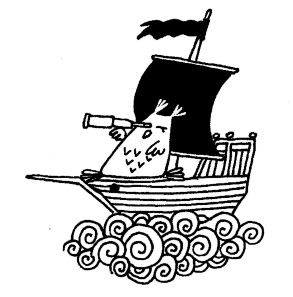
\includegraphics[scale=0.5]{22}}
\end{figure}
\end{SBSection*}

\end{song}

%\twocolumn
\begin{song}{Ленинградская (Все расстояния)}{}{Песни у костра}{Песни у костра}{}{}

\Ch{Am}{Все} расстоянья когда-нибудь в круг замы\Ch{E}{ка}ются,\par
\Ch{E}{Все} из разлук обязательно \Ch{E7}{встре}чей кон\Ch{Am}{ча}ются;\par
Должны про\Ch{Dm}{плыть} вокруг Зем\Ch{G}{ли,}\par
Вернуться в \Ch{C}{га}вань кораб\Ch{F}{ли,}\par   
Все поез\Ch{Dm}{да} в свои вер\Ch{E}{нуть}ся горо\Ch{Am}{да.}\\
 
Шумный вокзал то встречает друзей , то прощается,\par
Мы расстаемся, но снова назад возвращаемся -\par
Чтоб снова встать в огромный круг,\par
И снова знать, что рядом друг ,\par
И песни петь, чтоб больше не было разлук.\\
 
Все расстоянья когда-нибудь в круг замыкаются,\par
Все из разлук обязательно встречей кончаются;\par
И через год, и через пять,\par
Мы с вами встретимся опять,\par
Ничто не сможет нашей дружбе помешать.\par

\end{song}

%\twocolumn
\begin{song}{Десять капель}{}{Танцы Минус}{Танцы Минус}{}{}

Проигрыш: (2 раза)\par 
\Ch{C}{} \Ch{E}{} \Ch{Am}{} \Ch{F}{} \Ch{C}{} \Ch{E}{} \Ch{Am}{} \Ch{F}{}

\Ch{C}{Де}сять капель дож\Ch{E}{дя} у тебя на пле\Ch{Am}{че}\par
Ты забыла свой \Ch{F}{зонт,} ты спешила ко \Ch{C}{мне.}\par
Десять капель дож\Ch{E}{дя} на плече у те\Ch{Am}{бя,}\par
Десять капель люб\Ch{F}{ви,} десять капель ог\Ch{C}{ня}\\

Припев:\\(Три первых слова в припеве дублируются вторым голосом)\par
\tt\Ch{C}{Т}воя\Ch{E}{} ладо\Ch{Am}{нь} горит\Ch{F}{} в моих руках\par
\tt\Ch{C}{Л}юбви\Ch{E}{ }пож\Ch{Am}{ар} горит в тво\Ch{F}{их} глазах\\

Проигрыш.\\

Время делает шаг, время делает круг\par
Мы забудем друзей, мы забудем подруг\par
Просто выпьем вина из любви и огня\par
Десять капель меня, десять капель тебя\\

Припев.\\

Голос твой в тишине околдует меня\par
Ярким жарким огнем стану я до утра\par
Ты прикажешь гори, и я вспыхну любя\par
В этом пламени ты, в этом пламени я.\par

\end{song}

%\twocolumn
\begin{song}{Макет}{}{Песни у костра}{Сказка}{}{}
sadfsfthanks,\par
\begin{SBOpGroup}
asdas\
\end{SBOpGroup}
\begin{SBSection*}fdf\end{SBSection*}
\begin{SBVerse*}\end{SBVerse*}
\begin{SBChorus*}\end{SBChorus*}

\begin{SBOccurs}{23}
dsf
\end{SBOccurs}

\begin{SBSection*}
\begin{figure}[b!]
\center{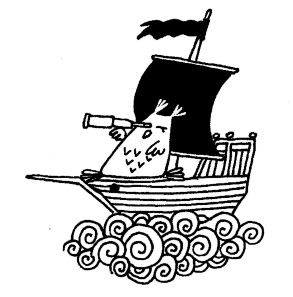
\includegraphics[scale=0.5]{22}}
\end{figure}
\end{SBSection*}
\end{song}

\mainmatter

\renewcommand{\footrulewidth}{0.0pt}
\renewcommand{\item}{\par\hangindent=40pt}
\renewcommand{\subitem}{\par\hangindent=40pt \hspace*{20pt}}
\renewcommand{\subsubitem}{\par\hangindent=40pt \hspace*{30pt}}

\newpage
\raggedright%\documentclass[a5paper,11pt]{book}
%\usepackage{fancyhdr}
%\usepackage[chordbk]{songbook}
%
%\usepackage[T2A]{fontenc}
%\usepackage[utf8]{inputenc}
%\usepackage[russian]{babel}
%
%\title{A Church Songbook}
%\author{}
%\date{Revised:  \RevDate}
%
%\newcommand{\RelDate}{13 November'19}
%\newcommand{\RevDate}{\today}

\documentclass[11pt,a5paper]{book}
\usepackage[a5paper]{geometry}
\usepackage[chordbk]{songbook}
\usepackage[T2A]{fontenc}
\usepackage[utf8]{inputenc}
\usepackage[russian]{babel}
\usepackage{cmap} % для работы поиска кириллицы в pdf

%\usepackage{amsmath,amsthm,amssymb}
%\usepackage{mathtext}


\usepackage[pdftex]{graphicx}
\usepackage{lscape}
%\usepackage{vmargin}
\usepackage{textcomp}
\usepackage{setspace}
%\usepackage{marvosym}
\usepackage{gensymb} %%%for \micro tag
\usepackage{upgreek} %%% \upmu
\usepackage{tipa}
\usepackage{phonetic}
%\usepackage[greek,english]{babel}
\usepackage{threeparttable}
\usepackage{multirow}
\usepackage{harvard}
\usepackage{longtable}
\renewcommand{\sectionmark}[1]{\markright{#1}}
\renewcommand{\chaptermark}[1]{\markboth{#1}{}}
\addto\captionsenglish{\renewcommand{\bibname}{References}}
\usepackage{latexsym,fancyhdr}

\newcommand{\RelDate}{26 Апреля'1984}
\newcommand{\RevDate}{\today}

%%%
% C.C.L.I. license number definition; for copyright licensing info.
% One of these macros will be manually inserted into the {CpyRt}
% parameter of the {song} environment.
%
%       \CCLInumber - The actual copyright license number.  Don't
%               insert this command in the {CpyRt} parameter, use one
%               of the others.
%       \CCLIed - Indicates a song falls under our CCLI license.
%       \NotCCLIed - Indicates a song doesn't fall under our CCLI
%               license.  Public Domain songs fall into this category.
%       \PGranted - We have received specific permission from the
%               copyright holder to use this song.
%       \PPending - We are in the process of obtaining permission to
%               use this song.
%%%
\newcommand{\CCLInumber}{Your CCLI Number}
\newcommand{\CCLIed}{{\CpyRtInfoFont (CCLI \CCLInumber)}}
\newcommand{\NotCCLIed}{\relax}
\newcommand{\PGranted}{\relax}
\newcommand{\PPending}{{\CpyRtInfoFont (Permission Pending)}}

%%%
% Title page information.
%%%
\title{ Сказочный песенник}
\author{}
\date{Созданно:  \RevDate}


%%%
% Define fonts to use in the headers and footers of the songbook.
%%%
\newcommand{\LHeadFont}{\normalsize}            % = cmr12  at 12pt
\newcommand{\CHeadFont}{\normalsize\rm}         % = cmr12  at 12pt
\newcommand{\RHeadFont}{\normalsize}            % = cmr12  at 12pt
\newcommand{\LFootFont}{\scriptsize}            % = cmr8   at  8pt
\newcommand{\CFootFont}{\tiny\myTinySF}         % = cmss8  at  8pt
\newcommand{\RFootFont}{\scriptsize}            % = cmr8   at  8pt

%%%
% Turn on and define fancy page heading/footing definition.
%%%
\pagestyle{fancy}

\ifChordBk
  % It's a words & chords songbook...
%  \addtolength{\headwidth}{\marginparsep}
%  \addtolength{\headwidth}{\marginparwidth}
  \renewcommand{\headrulewidth}{0.0pt}
  \renewcommand{\footrulewidth}{0.0pt}
%  \fancyhead[LE,RO]{\LHeadFont\emph{\leftmark\/}}
%  \fancyhead[CE,CO]{\CHeadFont\thepage}
  \fancyhead[RE,LO]{~}
\else\ifOverhead
  % It's an overhead...
  \renewcommand{\footrulewidth}{0pt}
  \renewcommand{\headrulewidth}{0pt}
  \fancyhead[LE,RO]{}
  \fancyhead[CE,CO]{}
  \fancyhead[RE,LO]{}
\else\ifWordBk
  % It's a words only songbook...
  \addtolength{\headwidth}{\marginparsep}
  \addtolength{\headwidth}{\marginparwidth}
  \renewcommand{\headrulewidth}{0.0pt}
  \renewcommand{\footrulewidth}{0.0pt}
  \fancyhead[LE,RO]{\LHeadFont A Church Songbook}
  \fancyhead[CE,CO]{\CHeadFont\thepage}
  \fancyhead[RE,LO]{\RHeadFont\RelDate}
\fi\fi\fi

%\fancyfoot[LE,RO]{\LFootFont Property of The Church}
%\ifSongEject
%  \fancyfoot[CE,CO]{\CFootFont \RevDate}
%\else
%  \fancyfoot[CE,CO]{\CFootFont}
%\fi
%\fancyfoot[RE,LO]{\RFootFont Material used by permission.}

%%%
% Turn on/off index-file generation.  Uncomment the \makeindex line to
% turn index generation on;  comment it out to turn index generation
% off.
%%%
\makeTitleIndex         %% Title and First Line Index.
\makeTitleContents      %% Table of Contents.
\makeKeyIndex           %% Index of song by key.
\graphicspath{{img/}} % папка с картинками
\DeclareGraphicsExtensions{.pdf,.png,.jpg} % форматы, которые будем считать картинками

%\newenvironment{song}[7][Y]{
%% Comment markers to negate
%\if#1Y\ExcludeSongfalse\else\ExcludeSongtrue\fi% the newline.
%\ifPrintAllSongs\ExcludeSongfalse\fi
%\SongMarkboth{\relax}{\relax}
%\SBinSongEnvtrue
%\renewcommand{\SBinSongEnv}{\True}
%\ifWordsOnly
%	\setlength{\parindent}{0pt}
%\fi

%%%
% Redefine fonts from SongBook style that I don't like.
%%%
\font\myTinySF=cmss8 at 8pt
\renewcommand{\CpyRtInfoFont}{\tiny\myTinySF}


%
%\font\myTinySF=cmss8    at  8pt
%\font\myHugeSF=cmssbx10 at 25pt
%\renewcommand{\CpyRtInfoFont}{\tiny\myTinySF}
%\newcommand{\myTitleFont}{\Huge\myHugeSF}
%\newcommand{\mySubTitleFont}{\large\sf}

%%% Работа с русским языком
%\usepackage[no-math]{fontspec}      %% подготавливает загрузку шрифтов Open Type, True Type и др.
%\defaultfontfeatures{Ligatures={TeX},Renderer=Basic}  %% свойства шрифтов по умолчанию
%\setmainfont[Ligatures={TeX,Historic}]{Times New Roman} %% задаёт основной шрифт документа
%\setsansfont{Helvetica Neue}                    %% задаёт шрифт без засечек

%\newfontfamily{\allods}{AllodsWest}

\newcommand{\SBPubDomm}{~}
\renewcommand{\CpyRt}[3][Y]{%
\if#1Y\begin{center}\fi
\if\blank{#2}%
\if\blank{#3}%
{\CpyRtFont\copyright \SBUnknownTag{} \CpyRtInfoFont}%
\else
{\CpyRtFont\copyright \SBUnknownTag{} \CpyRtInfoFont #3}%
\fi%
\else%
\ifthenelse{\equal{#2}{\SBPubDomm}}
{%then
{\CpyRtFont #2 \CpyRtInfoFont #3}%
}{%else
{\CpyRtFont #2 \CpyRtInfoFont #3}%
}%fi
\fi%
\if#1Y\end{center}\fi
}


\newcommand{\SBUnknownTagg}{~}
\renewcommand{\WAndM}[2][Y]{~}
\renewcommand{\WAndM}[2][Y]{%
\if#1Y\begin{center}\fi
\if\blank{#2}%
{\SBUnknownTagg}%
\else
{~}%
\fi
\if#1Y\end{center}\fi
}

\renewcommand{\STitle}[3][Y]{%
\setcounter{SBVerseCnt}{0}%
\setcounter{SBSectionCnt}{0}%
\ifExcludeSong\relax%
	\else\keyIndex{{\protect\sbChord#3\protect\relax} -- #2}{\theSBSongCnt}\fi%
	\vspace{\SpaceAboveSTitle}%
\if#1Y\begin{center}\fi
	{}{\STitleFont\LARGE #2}%
	\ifWordsOnly\relax\else\fi%
	\if#1Y\end{center}\fi
\STitleMarkboth{#2}{\relax}%
}


%\renewenvironment{SBOpGroup}{%
%	\sbSetsbBaselineSkipAmt%
%	\bgroup%
%	\begin{list}{\hbox{}}
%	  {\setlength {\leftmargin}
%		{\HangAmt}
%		\setlength{\itemindent}
%			{-\HangAmt}
%		\setlength{\listparindent}{-\HangAmt}
%		\setlength{\topsep}{0pt}
%		\setlength{\parsep}{0pt}
%		\setlength{\labelwidth}{0pt}
%		\setlength{\labelsep}{0pt}
%		\setlength{\baselineskip} {\sbBaselineSkipAmt}
%	}%\item}
%{\end{list}%
\newcommand{\SBChorusTagg}{Припев}
\renewenvironment{SBChorus}{%
\sbSetsbBaselineSkipAmt%
\bgroup%
\SBChorusMarkright{\SBChorusTag}
\begin{list}{{\SBChorusTagFont\SBChorusTagg}}
{\setlength {\leftmargin}
{\LeftMarginSBChorus + \HangAmt}
\setlength{\itemindent}
{-\HangAmt}
\setlength{\listparindent}{-\HangAmt}
\setlength{\parsep}
{0pt}
\setlength{\baselineskip} {\sbBaselineSkipAmt}
}%
\item}
{\end{list}%
\egroup%
\SpaceAfterChorus%
}

\renewcommand{\tt}{\indent \indent}
%\renewcommand{\nt}{\noindent}


\usepackage{amsmath}

\makeArtistIndex
\makeTitleIndex         %% Title and First Line Index.
\makeTitleContents      %% Table of Contents.
\makeKeyIndex           %% Index of song by key.
%\usepackage{printallsongs}

\begin{document} 
\maketitle

\mainmatter


\begin{song}{Вожатский гимн}{}{Сказка}{Сказка}{}{}

По \Ch{Am}{ла}герю подъём, нас горн зовёт!\par
Забудь о том, что ночь была бес\Ch{C}{сон}ною\par
Смо\Ch{Dm}{чи} водою \Ch{G}{ве}ки воспа\Ch{C}{лён}\Ch{F}{ные}\par    
По\Ch{Dm}{вя}зывай свой \Ch{E}{галс}тук — и впе\Ch{Am (A7)}{рёд!}\par
Смо\Ch{Dm}{чи} водою \Ch{G}{ве}ки воспа\Ch{C}{лён}\Ch{F}{ные}\par    
По\Ch{Dm}{вя}зывай свой \Ch{E}{галс}тук — и впе\Ch{Am (A7)}{рёд!}\par

%	\begin{SBChorus*}
\ttНе\Ch{E}{про}сто воспитывать \Ch{Am}{но}вых людей,\par
\ttНу \Ch{E}{что} ж, это наша с то\Ch{Am}{бою} свя\Ch{A7}{ты}ня.\par
\ttМой \Ch{Dm}{друг}, нам до\Ch{G}{ве}рили \Ch{C}{ду}ши де\Ch{F}{тей},\par
\ttИх \Ch{Dm}{ра}достный \Ch{Am}{смех} нам на\Ch{E}{гра}да от\Ch{Am}{ны}не.\par
\ttМой \Ch{Dm}{друг}, нам до\Ch{G}{ве}рили \Ch{C}{ду}ши де\Ch{F}{тей},\par
\ttИх \Ch{Dm}{ра}достный \Ch{Am}{смех} нам на\Ch{E}{гра}да от\Ch{Am}{ны}не.\\
%\end{SBChorus*}

Отбой, засыпает детвора.\par
Взгляни на их улыбки полусонные,\par
Пускай им снятся острова зелёные,\par
А нам опять работать до утра!\par
Пускай им снятся острова зелёные,\par
А нам опять работать до утра!\par

\tt И пусть от бессилья затихнешь не раз,\par
\ttИ голос усталый до хрипа натружен,\par
\ttПусть будут умней и счастливее нас\par
\ttТе дети, в которых вложили мы души!\par
\ttПусть будут умней и счастливее нас\par
\ttТе дети, в которых вложили мы души!

\end{song}

\begin{song}{Сказка в неглиже}{}{Сказка}{Сказка}{}{}

Есть у \Ch{C}{каж}дого добрая сказка в ду\Ch{F}{ше,}\par 
Надо \Ch{G}{толь}ко прочесть этой сказки стра\Ch{C}{ни}цы.\par
В тиши\Ch{C}{не}, разо\Ch{C7}{де}тая вся в негли\Ch{F}{же,}\par
Пусть на\Ch{G}{ве}ки она, пусть на\Ch{F}{ве}ки она сохра\Ch{C}{ни}тся. \Ch{C7}{ }\par 
В тиши\Ch{F}{не,} разо\Ch{G}{де}тая вся в негли\Ch{C}{же,} \Ch{Am}{}\par
Пусть на\Ch{F}{ве}ки она, пусть на\Ch{G}{ве}ки она сохра\Ch{C}{ни}тся.\\


\ttЭту сказку пред другом раскрыть поспеши,\par
\ttА врагу не спеши эту сказку поведать.\par
\ttПусть растут и читают ее малыши.\par
\ttБудь добрей, и тебя минут всякие беды.\par
\ttПусть растут и читают ее малыши.\par
\ttБудь добрей, и тебя минут всякие беды.\\


\Ch{C7}{}Будет \Ch{F}{мно}го распутий, \Ch{G}{до}рог и тре\Ch{C}{вог.}\Ch{Am}{}\par
На вис\Ch{F}{ки} твои ляжет \Ch{G}{не}тающий \Ch{C}{ин}ей, \Ch{C7}{}\par
И пой\Ch{F}{мёшь,} научившись чи\Ch{G}{тать} между \Ch{C}{строк:} \Ch{Am}{}\par
Даже \Ch{F}{гнус}ный злодей \Ch{G}{в} этой сказке не\Ch{C}{ви}нен. \Ch{C7}{}\par
И пой\Ch{F}{мёшь,} научившись чи\Ch{G}{тать} между ст\Ch{C}{рок:} \Ch{A}{}\par
Даже \Ch{F}{гнус}ный злодей \Ch{G}{в} этой сказке не\Ch{C}{ви}нен.\\

\Ch{C}{} \Ch{G}{} \Ch{F}{} \Ch{G}{} \Ch{C}{} \Ch{C7}{}\par
\Ch{C}{} \Ch{G}{} \Ch{F}{} \Ch{G}{} \Ch{C}{}
\end{song}

%\twocolumn
\begin{song}{Вожатский марш}{}{Сказка}{Сказка}{}{}

Есть на\Ch{Am}{род} у нас весёлый,\par
Самой \Ch{C}{луч}шей в мире пробы,\par
Песни \Ch{G}{петь} всегда мас\Ch{C}{так.}\Ch{A7}{}\par
Он всег\Ch{Dm}{да} всего добьётся,\par
Он Вожа\Ch{Am}{ты}ми зовётся,\par
\Ch{E}{Так} и только \Ch{Am (A7)}{так!}\par
Он всег\Ch{Dm}{да} всего добьётся,\par
Он Во\Ch{Am}{жа}тыми зовётся,\par
\Ch{E}{Так} и только \Ch{Am (A7)}{так!}\\

Домосед привязан к дому\par
И по случаю такому,\par
Он из дома — ни на шаг!\par
А вожатый — он в дороге,\par
Он готов в огонь и в воду,\par
Так и только так!\par
А вожатый — он в дороге,\par
Он готов в огонь и в воду,\par
Так и только так!\\
\newpage
Жадный денежки считает,\par
Все считает и считает,\par
К пятаку кладет пятак.\par
А вожатый деньги тратит,\par
Не боясь, что их не хватит,\par
Так и только так!\par
А вожатый деньги тратит,\par
Не боясь, что их не хватит,\par
Так и только так!\\

Холостяк в любовь не верит,\par
Все не верит и не верит,\par
Потому что холостяк.\par
А вожатых не влюблённых\par
Не найдёшь определённо,\par
Так и только так!\par
А вожатых не влюблённых\par
Не найдёшь определённо,\par
Так и только так!\par

\begin{SBSection*}
\begin{figure}[b!]
\center{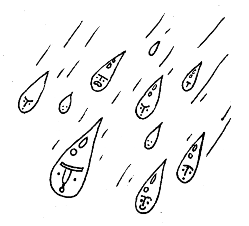
\includegraphics[scale=0.5]{16}}
\end{figure}
\end{SBSection*}
\end{song}

%\twocolumn
\begin{song}{Двадцать дней}{}{Сказка}{Сказка}{}{}


Двадцать дн\Ch{Dm}{ей} – это смена без дня.\par
“Маловато”,– вам скажут друзь\Ch{Gm}{я,}\par
А вожатый отв\Ch{C}{ет}ит люб\Ch{F}{ой}:\par
Это ср\Ch{Gm}{ок} очень д\Ch{A}{аж}е больш\Ch{Dm}{ой!}\\
 

Припев:\par
\ttМожно з\Ch{Gm C}{а-а-а-а} него усп\Ch{Dm}{ет}ь,\par
\ttНаприм\Ch{Gm}{ер,} полмилли\Ch{A}{он}а песен сп\Ch{Dm}{еть,}\par
\ttНо не к\Ch{Gm}{ажд}ый ведь поймет,\par
\ttКак так быстро раскрыв\Ch{A}{ат}ься может р\Ch{Dm}{от!}\\


Для полярника это не срок:\par
Не успеет просохнуть носок.\par
А вожатый успеет подряд \par
Вымыть, высушить сотню ребят!\\

Припев:\par
\ttВедь за смену, как за год \par
\ttСтолько разных мелочей произойдет,\par
\ttНо пока что нам везет,\par
\ttНас начальство для чего-то бережёт.\\


\newpage
Хоть и длинными кажутся дни,\par
Но как миг пролетели они.\par
Будешь долго потом вспоминать,\par
Как в отбой ты любил слово «СПАААТЬ!!!»\\

Припев:\par
\tt          	— Говорят за двадцать дней \par
\tt          	Все узнаешь о напарнице своей…\par
\tt          	— Только это ерунда,\par
\tt          	Обо всем ты не узнаешь никогда!\\

Смена вряд ли даст ответ:\par
Ты нашел свое призванье или нет.\par
Так что надо продолжать,\par
Двадцать раз по двадцать суток отсчитать!\\

\begin{SBSection*}
\begin{figure}[b!]
\center{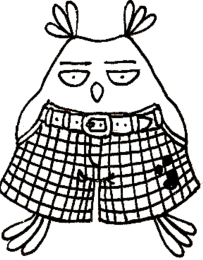
\includegraphics[scale=0.5]{17}}
\end{figure}
\end{SBSection*}

\end{song}

%\twocolumn
\begin{song}{Непогода}{}{Павел Смеян}{Павел Смеян}{}{}

\Ch{D}{Из}менения в природе \Ch{G}{пр}оисходят г\Ch{A}{од} от года,\par
\Ch{D}{Не}погода нынче в моде,\Ch{G}{} н\Ch{F#7}{епог}ода, непогода,\par
\Ch{}Hm{Слов}но из вод\Ch{F#7}{опро}вода \Ch{D7}{ль}ёт на нас с неб\Ch{G}{ес} во\Ch{Hm}{да…}\par
Полг\Ch{G}{од}а плох\Ch{A}{ая} пог\Ch{D}{од}а, \Ch{Hm}{пол}го\Ch{G}{да} — совс\Ch{A}{ем} нику\Ch{D}{да}.\par
Полг\Ch{G}{од}а плох\Ch{A}{ая} пог\Ch{D}{од}а, \Ch{Hm}{пол}го\Ch{G}{да} — сов\Ch{F#7}{сем} нику\Ch{Hm}{да.}\\


\SBChorusTagg:\par
\ttНикуда, нику\Ch{Em}{да н}ельз\Ch{A}{я} укр\Ch{D}{ы}ться н\Ch{Hm}{ам,}\par
\ttНо откладывать ж\Ch{Em}{изнь} ни\Ch{A}{как} нель\Ch{D}{зя}, \Ch{Hm}{}\par
\ttНикуда, нику\Ch{Em}{да, н}о зн\Ch{A}{ай}, что гд\Ch{D}{е}-то т\Ch{Hm}{ам}\par
\ttКто-то ищет теб\Ch{G}{я} сре\Ch{F#7}{ди д}ожд\Ch{Hm}{я.} \Ch{A}{}\\


Грома грозные раскаты от заката до восхода,\par
За грехи людские плата — непогода, непогода,\par
Не ангина, не простуда, посерьёзнее беда.\par
Полгода плохая погода, полгода — совсем никуда\par,
Полгода плохая погода, полгода — совсем никуда.\\\


\SBChorusTagg:\par
\ttНикуда, нику\Ch{Em}{да н}ельз\Ch{A}{я} укр\Ch{D}{ы}ться н\Ch{Hm}{ам,}\par
\ttНо откладывать ж\Ch{Em}{изнь} ни\Ch{A}{как} нель\Ch{D}{зя}, \Ch{Hm}{}\par
\ttНикуда, нику\Ch{Em}{да, н}о зн\Ch{A}{ай}, что гд\Ch{D}{е}-то т\Ch{Hm}{ам}\par
\ttКто-то ищет теб\Ch{G}{я} сре\Ch{F#7}{ди д}ожд\Ch{Hm}{я.} \Ch{A}{}\\


\end{song}

%\twocolumn
\begin{song}{Птенцы}{}{Сказка}{Сказка}{}{}

\Ch{Am}{}  \Ch{Am}{}

Как птенцы из гнез\Ch{Dm}{да} мы \Ch{E}{вы}па\Ch{Am}{ли.}\par
Ты не бойся при\Ch{Dm}{хо}да \Ch{G}{ве}че\Ch{C}{ра.}\par
Под та\Ch{A7}{ки}ми боль\Ch{F}{ши}ми \Ch{A7}{ли}па\Ch{Dm}{ми}\par
Нам с то\Ch{F}{бой} опа\Ch{Dm}{сать}ся \Ch{F}{не}\Ch{E}{че}\Ch{Am}{го.}\\
 
Под такими густыми звёздами -\par
Разве их не для нас рассыпали,\par
Мы не против гнездовья - просто мы\par
Из него ненароком выпали.\\

Это только вначале кажется,\par
Что без дома прожить нельзя никак,\par
Что важней пропитанья кашица,\par
Чем огромные звёзды на небе.\\

Ты не бойся ни тьмы, ни холода.\par
Будет день и найдётся пища нам,\par
Мы ещё пролетим над городом\par
На крыле до небес возвышенном.\\

Пролетим ещё - эка невидаль\par
Над Нью-Йорком, Парижем, Триполи\par
И над липой, откуда некогда,\par
Как птенцы из гнезда мы выпали.\\

Как птенцы из гнезда мы выпали.\par
Ты не бойся прихода вечера.\par
Под такими большими липами\par
Нам с тобой опасаться нечего.\\

\end{song}

%\twocolumn
\begin{song}{Продавец зонтиков}{}{Веня Дркин}{Веня Дркин}{}{}

\Ch{Am}{Город} этот выдумал о\Ch{Dm}{дин} художник,\par
\Ch{G}{Лю}ди в нем не знали, что та\Ch{C}{ко}е дождик.\par
\Ch{A7}{Про}сто не слыхали, что та\Ch{Dm}{ко}е зонтик –\par
\Ch{E7}{Вот} такие люди жили в \Ch{Am}{го}роде том.\par
И один чудак, в старый плащ одетый,\par
Продавал там зонтики зимой и летом,\par
Продавал там зонтики зимой и летом\par
И такую песенку он напевал:\\

\SBChorusTagg:\par
\tt“Господа, купите зонтик.\par
\ttБелый зонтик, красный зонтик,\par
\ttЖелтый зонтик, синий зонтик –\par
\ttМожет пригодится вам.”\\

Были домики у них из пластилина,\par
Из пустых коробочек автомашины,\par
И, не опасаясь никакой ангины,\par
Маленькие люди жили в городе том.\par
Маленькие были у людей заботы:\par
Шли они в кино или в театр с работы.\par
Вечером в подъезде целовался кто-то.\par
Все шутили и смеялись над стариком.\\


\SBChorusTagg.\\

\newpage

Маленькое небо как-то вдруг намокло,\par
В крошечных домишках задрожали стекла,\par
И огромный дождь пошел гулять по крышам,\par
Сразу все схватили насморк в городе том.\par
Вспомнили тут люди о торговце старом,\par
Кинулись искать его по всем базарам,\par
Но исчез торговец со своим товаром.\par
Только песенка осталась в память о нем:\\

\SBChorusTagg.\par

\begin{SBSection*}
\begin{figure}[b!]
\center{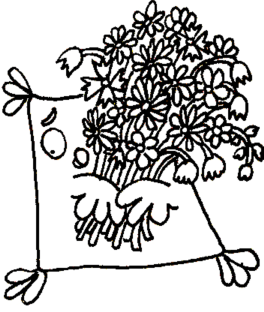
\includegraphics[scale=0.5]{15}}
\end{figure}
\end{SBSection*}

\end{song}

%\twocolumn
\begin{song}{Белая гвардия}{}{Белая гвардия}{Белая гвардия}{}{}

Проигрыш: (2 раза)\par 
\Ch{Am}{} \Ch{D}{} \Ch{G}{} \Ch{C}{} \Ch{Am}{} \Ch{H7}{} \Ch{Em}\\

\Ch{Em}{Белая} гвардия, белый снег,\par
\Ch{Am7}{Белая} музыка революций.\par
\Ch{D7}{Белая} женщина, нервный смех,\par
\Ch{G}{Белого} платья слегка коснуться.\par
 
Белой рукой распахнуть окно,\par
Белого света в нем не видя.\par
Белое выпить до дна вино,\par
В красную улицу в белом выйти.\\

Припев:\par
\ttКог\Ch{Em}{да} ты вернешься,\par
\ttВсе будет и\Ch{Am}{на}че, и нам бы узнать друг друга,\par
\ttКог\Ch{D7}{да} ты вернешься,\par
\ttА я не же\Ch{G}{на} и даже \Ch{H7}{не} подруга.\par
\ttКог\Ch{C}{да} ты вернешься,\par
\ttКо мне, так без\Ch{Am}{ум}но тебя любившей в прошлом,\par
\tt\Ch{D7}{Ко}гда ты вернешься -\par
\ttУвидишь, что ж\Ch{G}{ре}бий давно и не \Ch{E7}{нами} брошен.\\

Проигрыш.\\
 
\newpage
Сизые сумерки прошлых лет\par
Робко крадутся по переулкам.\par
В этом окне еле брезжит свет,\par
Ноты истрепаны, звуки гулки.\par
Тонкие пальцы срывают аккорд...\par
Нам не простят безрассудного дара.\par
Бьются в решетку стальных ворот\par
Пять океанов земного шара.\\

Припев. \par
Проигрыш.\\
 
Красный трамвай простучал в ночи,\par
Красный закат догорел в бокале,\par
Красные-красные кумачи\par
С красных деревьев на землю упали.\par
Я не ждала тебя в октябре,\par
Виделись сны, я листала сонник:\par
Красные лошади на заре\par
Били копытами о подоконник.\\

Припев:\par
\ttКогда ты вернешься,\par
\ttВсе будет иначе, и нам бы узнать друг друга,\par
\ttКогда ты вернешься,\par
\ttА я не жена и даже не подруга.\par
\ttКогда ты вернешься,\par
\ttВернешься в наш город обетованный,\par
\ttКогда ты вернешься -\par
\ttТакой невозможный и такой желанный?\\

Проигрыш.\par

\end{song}

%\twocolumn
\begin{song}{Перевал}{}{Песни у костра}{Песни у костра}{}{}


\Ch{Am}{Про}сто нечего нам \Ch{Dm}{боль}ше терять\par
\Ch{E}{Всё} нам вспомнится на \Ch{Am}{Страшном} суде.\par
Эта ночь легла, как \Ch{Dm}{тот} перевал,\par
\Ch{G}{За} которым испол\Ch{C}{нень}е надежд.\par
\Ch{A7}{Про}сто прожитое—про\Ch{Dm}{жи}то зря, \Ch{G}{}\par
Но не в этом, пони\Ch{C}{мае}шь ли, соль… \Ch{Am}{}\par
Слышишь, падают дож\Ch{Dm}{ди} октября.\par
\Ch{E}{Ви}дишь, старый дом сто\Ch{Am}{ит} средь лесов.\\

Мы затопим в доме печь, в доме печь,\par
Мы гитару позовем со стены.\par
Просто нечего нам больше беречь,\par
Ведь за нами все мосты сожжены.\par
Все мосты, все перекрёстки дорог,\par
Все прошёптанные тайны в ночи.\par
Каждый сделал все, что смог, все, что смог,\par
Мы об этом помолчим, помолчим.\\


И луна взойдет заплывшей свечой,\par
Ставни скрипнут  на ветру, на ветру.\par
Ах, как я тебя люблю горячо,\par
Это годы не сотрут, не сотрут.\par
Мы оставшихся друзей соберем,\par
Мы набьем картошкой старый рюкзак,\par
Люди спросят: "Что за шум, что за гам?"\par
Мы ответим: "Просто так,  просто так”...\\

\newpage

    Просто так идут дожди в октябре,\par
    И потеряны от счастья ключи.\par
    Это всё, конечно, мне, конечно, мне,\par
    Но об этом помолчим, помолчим.\par
    Просто прожитое—прожито зря,\par
    Но не в этом, понимаешь ли, соль…\par
    Слышишь, падают дожди октября.\par
    Видишь, старый дом стоит средь лесов.\par


\begin{SBSection*}
\begin{figure}[b!]
\center{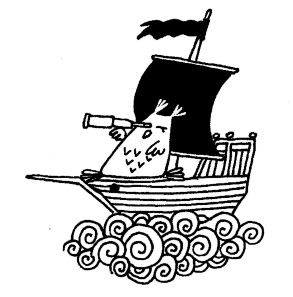
\includegraphics[scale=0.5]{22}}
\end{figure}
\end{SBSection*}

\end{song}

%\twocolumn
\begin{song}{Ленинградская (Все расстояния)}{}{Песни у костра}{Песни у костра}{}{}

\Ch{Am}{Все} расстоянья когда-нибудь в круг замы\Ch{E}{ка}ются,\par
\Ch{E}{Все} из разлук обязательно \Ch{E7}{встре}чей кон\Ch{Am}{ча}ются;\par
Должны про\Ch{Dm}{плыть} вокруг Зем\Ch{G}{ли,}\par
Вернуться в \Ch{C}{га}вань кораб\Ch{F}{ли,}\par   
Все поез\Ch{Dm}{да} в свои вер\Ch{E}{нуть}ся горо\Ch{Am}{да.}\\
 
Шумный вокзал то встречает друзей , то прощается,\par
Мы расстаемся, но снова назад возвращаемся -\par
Чтоб снова встать в огромный круг,\par
И снова знать, что рядом друг ,\par
И песни петь, чтоб больше не было разлук.\\
 
Все расстоянья когда-нибудь в круг замыкаются,\par
Все из разлук обязательно встречей кончаются;\par
И через год, и через пять,\par
Мы с вами встретимся опять,\par
Ничто не сможет нашей дружбе помешать.\par

\end{song}

%\twocolumn
\begin{song}{Десять капель}{}{Танцы Минус}{Танцы Минус}{}{}

Проигрыш: (2 раза)\par 
\Ch{C}{} \Ch{E}{} \Ch{Am}{} \Ch{F}{} \Ch{C}{} \Ch{E}{} \Ch{Am}{} \Ch{F}{}

\Ch{C}{Де}сять капель дож\Ch{E}{дя} у тебя на пле\Ch{Am}{че}\par
Ты забыла свой \Ch{F}{зонт,} ты спешила ко \Ch{C}{мне.}\par
Десять капель дож\Ch{E}{дя} на плече у те\Ch{Am}{бя,}\par
Десять капель люб\Ch{F}{ви,} десять капель ог\Ch{C}{ня}\\

Припев:\\(Три первых слова в припеве дублируются вторым голосом)\par
\tt\Ch{C}{Т}воя\Ch{E}{} ладо\Ch{Am}{нь} горит\Ch{F}{} в моих руках\par
\tt\Ch{C}{Л}юбви\Ch{E}{ }пож\Ch{Am}{ар} горит в тво\Ch{F}{их} глазах\\

Проигрыш.\\

Время делает шаг, время делает круг\par
Мы забудем друзей, мы забудем подруг\par
Просто выпьем вина из любви и огня\par
Десять капель меня, десять капель тебя\\

Припев.\\

Голос твой в тишине околдует меня\par
Ярким жарким огнем стану я до утра\par
Ты прикажешь гори, и я вспыхну любя\par
В этом пламени ты, в этом пламени я.\par

\end{song}

%\twocolumn
\begin{song}{Макет}{}{Песни у костра}{Сказка}{}{}
sadfsfthanks,\par
\begin{SBOpGroup}
asdas\
\end{SBOpGroup}
\begin{SBSection*}fdf\end{SBSection*}
\begin{SBVerse*}\end{SBVerse*}
\begin{SBChorus*}\end{SBChorus*}

\begin{SBOccurs}{23}
dsf
\end{SBOccurs}

\begin{SBSection*}
\begin{figure}[b!]
\center{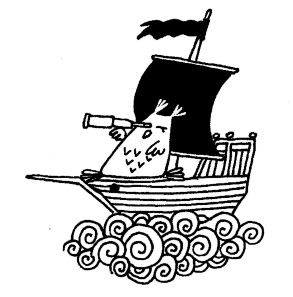
\includegraphics[scale=0.5]{22}}
\end{figure}
\end{SBSection*}
\end{song}

\mainmatter

\renewcommand{\footrulewidth}{0.0pt}
\renewcommand{\item}{\par\hangindent=40pt}
\renewcommand{\subitem}{\par\hangindent=40pt \hspace*{20pt}}
\renewcommand{\subsubitem}{\par\hangindent=40pt \hspace*{30pt}}

\newpage
\raggedright%\documentclass[a5paper,11pt]{book}
%\usepackage{fancyhdr}
%\usepackage[chordbk]{songbook}
%
%\usepackage[T2A]{fontenc}
%\usepackage[utf8]{inputenc}
%\usepackage[russian]{babel}
%
%\title{A Church Songbook}
%\author{}
%\date{Revised:  \RevDate}
%
%\newcommand{\RelDate}{13 November'19}
%\newcommand{\RevDate}{\today}

\documentclass[11pt,a5paper]{book}
\usepackage[a5paper]{geometry}
\usepackage[chordbk]{songbook}
\usepackage[T2A]{fontenc}
\usepackage[utf8]{inputenc}
\usepackage[russian]{babel}
\usepackage{cmap} % для работы поиска кириллицы в pdf

%\usepackage{amsmath,amsthm,amssymb}
%\usepackage{mathtext}


\usepackage[pdftex]{graphicx}
\usepackage{lscape}
%\usepackage{vmargin}
\usepackage{textcomp}
\usepackage{setspace}
%\usepackage{marvosym}
\usepackage{gensymb} %%%for \micro tag
\usepackage{upgreek} %%% \upmu
\usepackage{tipa}
\usepackage{phonetic}
%\usepackage[greek,english]{babel}
\usepackage{threeparttable}
\usepackage{multirow}
\usepackage{harvard}
\usepackage{longtable}
\renewcommand{\sectionmark}[1]{\markright{#1}}
\renewcommand{\chaptermark}[1]{\markboth{#1}{}}
\addto\captionsenglish{\renewcommand{\bibname}{References}}
\usepackage{latexsym,fancyhdr}

\newcommand{\RelDate}{26 Апреля'1984}
\newcommand{\RevDate}{\today}

%%%
% C.C.L.I. license number definition; for copyright licensing info.
% One of these macros will be manually inserted into the {CpyRt}
% parameter of the {song} environment.
%
%       \CCLInumber - The actual copyright license number.  Don't
%               insert this command in the {CpyRt} parameter, use one
%               of the others.
%       \CCLIed - Indicates a song falls under our CCLI license.
%       \NotCCLIed - Indicates a song doesn't fall under our CCLI
%               license.  Public Domain songs fall into this category.
%       \PGranted - We have received specific permission from the
%               copyright holder to use this song.
%       \PPending - We are in the process of obtaining permission to
%               use this song.
%%%
\newcommand{\CCLInumber}{Your CCLI Number}
\newcommand{\CCLIed}{{\CpyRtInfoFont (CCLI \CCLInumber)}}
\newcommand{\NotCCLIed}{\relax}
\newcommand{\PGranted}{\relax}
\newcommand{\PPending}{{\CpyRtInfoFont (Permission Pending)}}

%%%
% Title page information.
%%%
\title{ Сказочный песенник}
\author{}
\date{Созданно:  \RevDate}


%%%
% Define fonts to use in the headers and footers of the songbook.
%%%
\newcommand{\LHeadFont}{\normalsize}            % = cmr12  at 12pt
\newcommand{\CHeadFont}{\normalsize\rm}         % = cmr12  at 12pt
\newcommand{\RHeadFont}{\normalsize}            % = cmr12  at 12pt
\newcommand{\LFootFont}{\scriptsize}            % = cmr8   at  8pt
\newcommand{\CFootFont}{\tiny\myTinySF}         % = cmss8  at  8pt
\newcommand{\RFootFont}{\scriptsize}            % = cmr8   at  8pt

%%%
% Turn on and define fancy page heading/footing definition.
%%%
\pagestyle{fancy}

\ifChordBk
  % It's a words & chords songbook...
%  \addtolength{\headwidth}{\marginparsep}
%  \addtolength{\headwidth}{\marginparwidth}
  \renewcommand{\headrulewidth}{0.0pt}
  \renewcommand{\footrulewidth}{0.0pt}
%  \fancyhead[LE,RO]{\LHeadFont\emph{\leftmark\/}}
%  \fancyhead[CE,CO]{\CHeadFont\thepage}
  \fancyhead[RE,LO]{~}
\else\ifOverhead
  % It's an overhead...
  \renewcommand{\footrulewidth}{0pt}
  \renewcommand{\headrulewidth}{0pt}
  \fancyhead[LE,RO]{}
  \fancyhead[CE,CO]{}
  \fancyhead[RE,LO]{}
\else\ifWordBk
  % It's a words only songbook...
  \addtolength{\headwidth}{\marginparsep}
  \addtolength{\headwidth}{\marginparwidth}
  \renewcommand{\headrulewidth}{0.0pt}
  \renewcommand{\footrulewidth}{0.0pt}
  \fancyhead[LE,RO]{\LHeadFont A Church Songbook}
  \fancyhead[CE,CO]{\CHeadFont\thepage}
  \fancyhead[RE,LO]{\RHeadFont\RelDate}
\fi\fi\fi

%\fancyfoot[LE,RO]{\LFootFont Property of The Church}
%\ifSongEject
%  \fancyfoot[CE,CO]{\CFootFont \RevDate}
%\else
%  \fancyfoot[CE,CO]{\CFootFont}
%\fi
%\fancyfoot[RE,LO]{\RFootFont Material used by permission.}

%%%
% Turn on/off index-file generation.  Uncomment the \makeindex line to
% turn index generation on;  comment it out to turn index generation
% off.
%%%
\makeTitleIndex         %% Title and First Line Index.
\makeTitleContents      %% Table of Contents.
\makeKeyIndex           %% Index of song by key.
\graphicspath{{img/}} % папка с картинками
\DeclareGraphicsExtensions{.pdf,.png,.jpg} % форматы, которые будем считать картинками

%\newenvironment{song}[7][Y]{
%% Comment markers to negate
%\if#1Y\ExcludeSongfalse\else\ExcludeSongtrue\fi% the newline.
%\ifPrintAllSongs\ExcludeSongfalse\fi
%\SongMarkboth{\relax}{\relax}
%\SBinSongEnvtrue
%\renewcommand{\SBinSongEnv}{\True}
%\ifWordsOnly
%	\setlength{\parindent}{0pt}
%\fi

%%%
% Redefine fonts from SongBook style that I don't like.
%%%
\font\myTinySF=cmss8 at 8pt
\renewcommand{\CpyRtInfoFont}{\tiny\myTinySF}


%
%\font\myTinySF=cmss8    at  8pt
%\font\myHugeSF=cmssbx10 at 25pt
%\renewcommand{\CpyRtInfoFont}{\tiny\myTinySF}
%\newcommand{\myTitleFont}{\Huge\myHugeSF}
%\newcommand{\mySubTitleFont}{\large\sf}

%%% Работа с русским языком
%\usepackage[no-math]{fontspec}      %% подготавливает загрузку шрифтов Open Type, True Type и др.
%\defaultfontfeatures{Ligatures={TeX},Renderer=Basic}  %% свойства шрифтов по умолчанию
%\setmainfont[Ligatures={TeX,Historic}]{Times New Roman} %% задаёт основной шрифт документа
%\setsansfont{Helvetica Neue}                    %% задаёт шрифт без засечек

%\newfontfamily{\allods}{AllodsWest}

\newcommand{\SBPubDomm}{~}
\renewcommand{\CpyRt}[3][Y]{%
\if#1Y\begin{center}\fi
\if\blank{#2}%
\if\blank{#3}%
{\CpyRtFont\copyright \SBUnknownTag{} \CpyRtInfoFont}%
\else
{\CpyRtFont\copyright \SBUnknownTag{} \CpyRtInfoFont #3}%
\fi%
\else%
\ifthenelse{\equal{#2}{\SBPubDomm}}
{%then
{\CpyRtFont #2 \CpyRtInfoFont #3}%
}{%else
{\CpyRtFont #2 \CpyRtInfoFont #3}%
}%fi
\fi%
\if#1Y\end{center}\fi
}


\newcommand{\SBUnknownTagg}{~}
\renewcommand{\WAndM}[2][Y]{~}
\renewcommand{\WAndM}[2][Y]{%
\if#1Y\begin{center}\fi
\if\blank{#2}%
{\SBUnknownTagg}%
\else
{~}%
\fi
\if#1Y\end{center}\fi
}

\renewcommand{\STitle}[3][Y]{%
\setcounter{SBVerseCnt}{0}%
\setcounter{SBSectionCnt}{0}%
\ifExcludeSong\relax%
	\else\keyIndex{{\protect\sbChord#3\protect\relax} -- #2}{\theSBSongCnt}\fi%
	\vspace{\SpaceAboveSTitle}%
\if#1Y\begin{center}\fi
	{}{\STitleFont\LARGE #2}%
	\ifWordsOnly\relax\else\fi%
	\if#1Y\end{center}\fi
\STitleMarkboth{#2}{\relax}%
}


%\renewenvironment{SBOpGroup}{%
%	\sbSetsbBaselineSkipAmt%
%	\bgroup%
%	\begin{list}{\hbox{}}
%	  {\setlength {\leftmargin}
%		{\HangAmt}
%		\setlength{\itemindent}
%			{-\HangAmt}
%		\setlength{\listparindent}{-\HangAmt}
%		\setlength{\topsep}{0pt}
%		\setlength{\parsep}{0pt}
%		\setlength{\labelwidth}{0pt}
%		\setlength{\labelsep}{0pt}
%		\setlength{\baselineskip} {\sbBaselineSkipAmt}
%	}%\item}
%{\end{list}%
\newcommand{\SBChorusTagg}{Припев}
\renewenvironment{SBChorus}{%
\sbSetsbBaselineSkipAmt%
\bgroup%
\SBChorusMarkright{\SBChorusTag}
\begin{list}{{\SBChorusTagFont\SBChorusTagg}}
{\setlength {\leftmargin}
{\LeftMarginSBChorus + \HangAmt}
\setlength{\itemindent}
{-\HangAmt}
\setlength{\listparindent}{-\HangAmt}
\setlength{\parsep}
{0pt}
\setlength{\baselineskip} {\sbBaselineSkipAmt}
}%
\item}
{\end{list}%
\egroup%
\SpaceAfterChorus%
}

\renewcommand{\tt}{\indent \indent}
%\renewcommand{\nt}{\noindent}


\usepackage{amsmath}

\makeArtistIndex
\makeTitleIndex         %% Title and First Line Index.
\makeTitleContents      %% Table of Contents.
\makeKeyIndex           %% Index of song by key.
%\usepackage{printallsongs}

\begin{document} 
\maketitle

\mainmatter


\begin{song}{Вожатский гимн}{}{Сказка}{Сказка}{}{}

По \Ch{Am}{ла}герю подъём, нас горн зовёт!\par
Забудь о том, что ночь была бес\Ch{C}{сон}ною\par
Смо\Ch{Dm}{чи} водою \Ch{G}{ве}ки воспа\Ch{C}{лён}\Ch{F}{ные}\par    
По\Ch{Dm}{вя}зывай свой \Ch{E}{галс}тук — и впе\Ch{Am (A7)}{рёд!}\par
Смо\Ch{Dm}{чи} водою \Ch{G}{ве}ки воспа\Ch{C}{лён}\Ch{F}{ные}\par    
По\Ch{Dm}{вя}зывай свой \Ch{E}{галс}тук — и впе\Ch{Am (A7)}{рёд!}\par

%	\begin{SBChorus*}
\ttНе\Ch{E}{про}сто воспитывать \Ch{Am}{но}вых людей,\par
\ttНу \Ch{E}{что} ж, это наша с то\Ch{Am}{бою} свя\Ch{A7}{ты}ня.\par
\ttМой \Ch{Dm}{друг}, нам до\Ch{G}{ве}рили \Ch{C}{ду}ши де\Ch{F}{тей},\par
\ttИх \Ch{Dm}{ра}достный \Ch{Am}{смех} нам на\Ch{E}{гра}да от\Ch{Am}{ны}не.\par
\ttМой \Ch{Dm}{друг}, нам до\Ch{G}{ве}рили \Ch{C}{ду}ши де\Ch{F}{тей},\par
\ttИх \Ch{Dm}{ра}достный \Ch{Am}{смех} нам на\Ch{E}{гра}да от\Ch{Am}{ны}не.\\
%\end{SBChorus*}

Отбой, засыпает детвора.\par
Взгляни на их улыбки полусонные,\par
Пускай им снятся острова зелёные,\par
А нам опять работать до утра!\par
Пускай им снятся острова зелёные,\par
А нам опять работать до утра!\par

\tt И пусть от бессилья затихнешь не раз,\par
\ttИ голос усталый до хрипа натружен,\par
\ttПусть будут умней и счастливее нас\par
\ttТе дети, в которых вложили мы души!\par
\ttПусть будут умней и счастливее нас\par
\ttТе дети, в которых вложили мы души!

\end{song}

\begin{song}{Сказка в неглиже}{}{Сказка}{Сказка}{}{}

Есть у \Ch{C}{каж}дого добрая сказка в ду\Ch{F}{ше,}\par 
Надо \Ch{G}{толь}ко прочесть этой сказки стра\Ch{C}{ни}цы.\par
В тиши\Ch{C}{не}, разо\Ch{C7}{де}тая вся в негли\Ch{F}{же,}\par
Пусть на\Ch{G}{ве}ки она, пусть на\Ch{F}{ве}ки она сохра\Ch{C}{ни}тся. \Ch{C7}{ }\par 
В тиши\Ch{F}{не,} разо\Ch{G}{де}тая вся в негли\Ch{C}{же,} \Ch{Am}{}\par
Пусть на\Ch{F}{ве}ки она, пусть на\Ch{G}{ве}ки она сохра\Ch{C}{ни}тся.\\


\ttЭту сказку пред другом раскрыть поспеши,\par
\ttА врагу не спеши эту сказку поведать.\par
\ttПусть растут и читают ее малыши.\par
\ttБудь добрей, и тебя минут всякие беды.\par
\ttПусть растут и читают ее малыши.\par
\ttБудь добрей, и тебя минут всякие беды.\\


\Ch{C7}{}Будет \Ch{F}{мно}го распутий, \Ch{G}{до}рог и тре\Ch{C}{вог.}\Ch{Am}{}\par
На вис\Ch{F}{ки} твои ляжет \Ch{G}{не}тающий \Ch{C}{ин}ей, \Ch{C7}{}\par
И пой\Ch{F}{мёшь,} научившись чи\Ch{G}{тать} между \Ch{C}{строк:} \Ch{Am}{}\par
Даже \Ch{F}{гнус}ный злодей \Ch{G}{в} этой сказке не\Ch{C}{ви}нен. \Ch{C7}{}\par
И пой\Ch{F}{мёшь,} научившись чи\Ch{G}{тать} между ст\Ch{C}{рок:} \Ch{A}{}\par
Даже \Ch{F}{гнус}ный злодей \Ch{G}{в} этой сказке не\Ch{C}{ви}нен.\\

\Ch{C}{} \Ch{G}{} \Ch{F}{} \Ch{G}{} \Ch{C}{} \Ch{C7}{}\par
\Ch{C}{} \Ch{G}{} \Ch{F}{} \Ch{G}{} \Ch{C}{}
\end{song}

%\twocolumn
\begin{song}{Вожатский марш}{}{Сказка}{Сказка}{}{}

Есть на\Ch{Am}{род} у нас весёлый,\par
Самой \Ch{C}{луч}шей в мире пробы,\par
Песни \Ch{G}{петь} всегда мас\Ch{C}{так.}\Ch{A7}{}\par
Он всег\Ch{Dm}{да} всего добьётся,\par
Он Вожа\Ch{Am}{ты}ми зовётся,\par
\Ch{E}{Так} и только \Ch{Am (A7)}{так!}\par
Он всег\Ch{Dm}{да} всего добьётся,\par
Он Во\Ch{Am}{жа}тыми зовётся,\par
\Ch{E}{Так} и только \Ch{Am (A7)}{так!}\\

Домосед привязан к дому\par
И по случаю такому,\par
Он из дома — ни на шаг!\par
А вожатый — он в дороге,\par
Он готов в огонь и в воду,\par
Так и только так!\par
А вожатый — он в дороге,\par
Он готов в огонь и в воду,\par
Так и только так!\\
\newpage
Жадный денежки считает,\par
Все считает и считает,\par
К пятаку кладет пятак.\par
А вожатый деньги тратит,\par
Не боясь, что их не хватит,\par
Так и только так!\par
А вожатый деньги тратит,\par
Не боясь, что их не хватит,\par
Так и только так!\\

Холостяк в любовь не верит,\par
Все не верит и не верит,\par
Потому что холостяк.\par
А вожатых не влюблённых\par
Не найдёшь определённо,\par
Так и только так!\par
А вожатых не влюблённых\par
Не найдёшь определённо,\par
Так и только так!\par

\begin{SBSection*}
\begin{figure}[b!]
\center{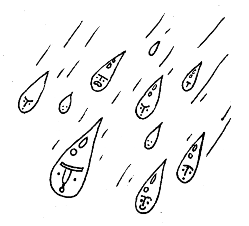
\includegraphics[scale=0.5]{16}}
\end{figure}
\end{SBSection*}
\end{song}

%\twocolumn
\begin{song}{Двадцать дней}{}{Сказка}{Сказка}{}{}


Двадцать дн\Ch{Dm}{ей} – это смена без дня.\par
“Маловато”,– вам скажут друзь\Ch{Gm}{я,}\par
А вожатый отв\Ch{C}{ет}ит люб\Ch{F}{ой}:\par
Это ср\Ch{Gm}{ок} очень д\Ch{A}{аж}е больш\Ch{Dm}{ой!}\\
 

Припев:\par
\ttМожно з\Ch{Gm C}{а-а-а-а} него усп\Ch{Dm}{ет}ь,\par
\ttНаприм\Ch{Gm}{ер,} полмилли\Ch{A}{он}а песен сп\Ch{Dm}{еть,}\par
\ttНо не к\Ch{Gm}{ажд}ый ведь поймет,\par
\ttКак так быстро раскрыв\Ch{A}{ат}ься может р\Ch{Dm}{от!}\\


Для полярника это не срок:\par
Не успеет просохнуть носок.\par
А вожатый успеет подряд \par
Вымыть, высушить сотню ребят!\\

Припев:\par
\ttВедь за смену, как за год \par
\ttСтолько разных мелочей произойдет,\par
\ttНо пока что нам везет,\par
\ttНас начальство для чего-то бережёт.\\


\newpage
Хоть и длинными кажутся дни,\par
Но как миг пролетели они.\par
Будешь долго потом вспоминать,\par
Как в отбой ты любил слово «СПАААТЬ!!!»\\

Припев:\par
\tt          	— Говорят за двадцать дней \par
\tt          	Все узнаешь о напарнице своей…\par
\tt          	— Только это ерунда,\par
\tt          	Обо всем ты не узнаешь никогда!\\

Смена вряд ли даст ответ:\par
Ты нашел свое призванье или нет.\par
Так что надо продолжать,\par
Двадцать раз по двадцать суток отсчитать!\\

\begin{SBSection*}
\begin{figure}[b!]
\center{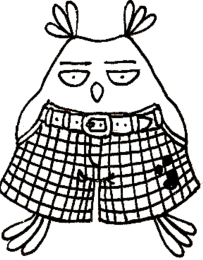
\includegraphics[scale=0.5]{17}}
\end{figure}
\end{SBSection*}

\end{song}

%\twocolumn
\begin{song}{Непогода}{}{Павел Смеян}{Павел Смеян}{}{}

\Ch{D}{Из}менения в природе \Ch{G}{пр}оисходят г\Ch{A}{од} от года,\par
\Ch{D}{Не}погода нынче в моде,\Ch{G}{} н\Ch{F#7}{епог}ода, непогода,\par
\Ch{}Hm{Слов}но из вод\Ch{F#7}{опро}вода \Ch{D7}{ль}ёт на нас с неб\Ch{G}{ес} во\Ch{Hm}{да…}\par
Полг\Ch{G}{од}а плох\Ch{A}{ая} пог\Ch{D}{од}а, \Ch{Hm}{пол}го\Ch{G}{да} — совс\Ch{A}{ем} нику\Ch{D}{да}.\par
Полг\Ch{G}{од}а плох\Ch{A}{ая} пог\Ch{D}{од}а, \Ch{Hm}{пол}го\Ch{G}{да} — сов\Ch{F#7}{сем} нику\Ch{Hm}{да.}\\


\SBChorusTagg:\par
\ttНикуда, нику\Ch{Em}{да н}ельз\Ch{A}{я} укр\Ch{D}{ы}ться н\Ch{Hm}{ам,}\par
\ttНо откладывать ж\Ch{Em}{изнь} ни\Ch{A}{как} нель\Ch{D}{зя}, \Ch{Hm}{}\par
\ttНикуда, нику\Ch{Em}{да, н}о зн\Ch{A}{ай}, что гд\Ch{D}{е}-то т\Ch{Hm}{ам}\par
\ttКто-то ищет теб\Ch{G}{я} сре\Ch{F#7}{ди д}ожд\Ch{Hm}{я.} \Ch{A}{}\\


Грома грозные раскаты от заката до восхода,\par
За грехи людские плата — непогода, непогода,\par
Не ангина, не простуда, посерьёзнее беда.\par
Полгода плохая погода, полгода — совсем никуда\par,
Полгода плохая погода, полгода — совсем никуда.\\\


\SBChorusTagg:\par
\ttНикуда, нику\Ch{Em}{да н}ельз\Ch{A}{я} укр\Ch{D}{ы}ться н\Ch{Hm}{ам,}\par
\ttНо откладывать ж\Ch{Em}{изнь} ни\Ch{A}{как} нель\Ch{D}{зя}, \Ch{Hm}{}\par
\ttНикуда, нику\Ch{Em}{да, н}о зн\Ch{A}{ай}, что гд\Ch{D}{е}-то т\Ch{Hm}{ам}\par
\ttКто-то ищет теб\Ch{G}{я} сре\Ch{F#7}{ди д}ожд\Ch{Hm}{я.} \Ch{A}{}\\


\end{song}

%\twocolumn
\begin{song}{Птенцы}{}{Сказка}{Сказка}{}{}

\Ch{Am}{}  \Ch{Am}{}

Как птенцы из гнез\Ch{Dm}{да} мы \Ch{E}{вы}па\Ch{Am}{ли.}\par
Ты не бойся при\Ch{Dm}{хо}да \Ch{G}{ве}че\Ch{C}{ра.}\par
Под та\Ch{A7}{ки}ми боль\Ch{F}{ши}ми \Ch{A7}{ли}па\Ch{Dm}{ми}\par
Нам с то\Ch{F}{бой} опа\Ch{Dm}{сать}ся \Ch{F}{не}\Ch{E}{че}\Ch{Am}{го.}\\
 
Под такими густыми звёздами -\par
Разве их не для нас рассыпали,\par
Мы не против гнездовья - просто мы\par
Из него ненароком выпали.\\

Это только вначале кажется,\par
Что без дома прожить нельзя никак,\par
Что важней пропитанья кашица,\par
Чем огромные звёзды на небе.\\

Ты не бойся ни тьмы, ни холода.\par
Будет день и найдётся пища нам,\par
Мы ещё пролетим над городом\par
На крыле до небес возвышенном.\\

Пролетим ещё - эка невидаль\par
Над Нью-Йорком, Парижем, Триполи\par
И над липой, откуда некогда,\par
Как птенцы из гнезда мы выпали.\\

Как птенцы из гнезда мы выпали.\par
Ты не бойся прихода вечера.\par
Под такими большими липами\par
Нам с тобой опасаться нечего.\\

\end{song}

%\twocolumn
\begin{song}{Продавец зонтиков}{}{Веня Дркин}{Веня Дркин}{}{}

\Ch{Am}{Город} этот выдумал о\Ch{Dm}{дин} художник,\par
\Ch{G}{Лю}ди в нем не знали, что та\Ch{C}{ко}е дождик.\par
\Ch{A7}{Про}сто не слыхали, что та\Ch{Dm}{ко}е зонтик –\par
\Ch{E7}{Вот} такие люди жили в \Ch{Am}{го}роде том.\par
И один чудак, в старый плащ одетый,\par
Продавал там зонтики зимой и летом,\par
Продавал там зонтики зимой и летом\par
И такую песенку он напевал:\\

\SBChorusTagg:\par
\tt“Господа, купите зонтик.\par
\ttБелый зонтик, красный зонтик,\par
\ttЖелтый зонтик, синий зонтик –\par
\ttМожет пригодится вам.”\\

Были домики у них из пластилина,\par
Из пустых коробочек автомашины,\par
И, не опасаясь никакой ангины,\par
Маленькие люди жили в городе том.\par
Маленькие были у людей заботы:\par
Шли они в кино или в театр с работы.\par
Вечером в подъезде целовался кто-то.\par
Все шутили и смеялись над стариком.\\


\SBChorusTagg.\\

\newpage

Маленькое небо как-то вдруг намокло,\par
В крошечных домишках задрожали стекла,\par
И огромный дождь пошел гулять по крышам,\par
Сразу все схватили насморк в городе том.\par
Вспомнили тут люди о торговце старом,\par
Кинулись искать его по всем базарам,\par
Но исчез торговец со своим товаром.\par
Только песенка осталась в память о нем:\\

\SBChorusTagg.\par

\begin{SBSection*}
\begin{figure}[b!]
\center{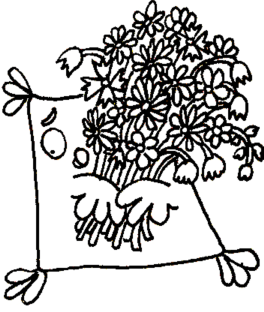
\includegraphics[scale=0.5]{15}}
\end{figure}
\end{SBSection*}

\end{song}

%\twocolumn
\begin{song}{Белая гвардия}{}{Белая гвардия}{Белая гвардия}{}{}

Проигрыш: (2 раза)\par 
\Ch{Am}{} \Ch{D}{} \Ch{G}{} \Ch{C}{} \Ch{Am}{} \Ch{H7}{} \Ch{Em}\\

\Ch{Em}{Белая} гвардия, белый снег,\par
\Ch{Am7}{Белая} музыка революций.\par
\Ch{D7}{Белая} женщина, нервный смех,\par
\Ch{G}{Белого} платья слегка коснуться.\par
 
Белой рукой распахнуть окно,\par
Белого света в нем не видя.\par
Белое выпить до дна вино,\par
В красную улицу в белом выйти.\\

Припев:\par
\ttКог\Ch{Em}{да} ты вернешься,\par
\ttВсе будет и\Ch{Am}{на}че, и нам бы узнать друг друга,\par
\ttКог\Ch{D7}{да} ты вернешься,\par
\ttА я не же\Ch{G}{на} и даже \Ch{H7}{не} подруга.\par
\ttКог\Ch{C}{да} ты вернешься,\par
\ttКо мне, так без\Ch{Am}{ум}но тебя любившей в прошлом,\par
\tt\Ch{D7}{Ко}гда ты вернешься -\par
\ttУвидишь, что ж\Ch{G}{ре}бий давно и не \Ch{E7}{нами} брошен.\\

Проигрыш.\\
 
\newpage
Сизые сумерки прошлых лет\par
Робко крадутся по переулкам.\par
В этом окне еле брезжит свет,\par
Ноты истрепаны, звуки гулки.\par
Тонкие пальцы срывают аккорд...\par
Нам не простят безрассудного дара.\par
Бьются в решетку стальных ворот\par
Пять океанов земного шара.\\

Припев. \par
Проигрыш.\\
 
Красный трамвай простучал в ночи,\par
Красный закат догорел в бокале,\par
Красные-красные кумачи\par
С красных деревьев на землю упали.\par
Я не ждала тебя в октябре,\par
Виделись сны, я листала сонник:\par
Красные лошади на заре\par
Били копытами о подоконник.\\

Припев:\par
\ttКогда ты вернешься,\par
\ttВсе будет иначе, и нам бы узнать друг друга,\par
\ttКогда ты вернешься,\par
\ttА я не жена и даже не подруга.\par
\ttКогда ты вернешься,\par
\ttВернешься в наш город обетованный,\par
\ttКогда ты вернешься -\par
\ttТакой невозможный и такой желанный?\\

Проигрыш.\par

\end{song}

%\twocolumn
\begin{song}{Перевал}{}{Песни у костра}{Песни у костра}{}{}


\Ch{Am}{Про}сто нечего нам \Ch{Dm}{боль}ше терять\par
\Ch{E}{Всё} нам вспомнится на \Ch{Am}{Страшном} суде.\par
Эта ночь легла, как \Ch{Dm}{тот} перевал,\par
\Ch{G}{За} которым испол\Ch{C}{нень}е надежд.\par
\Ch{A7}{Про}сто прожитое—про\Ch{Dm}{жи}то зря, \Ch{G}{}\par
Но не в этом, пони\Ch{C}{мае}шь ли, соль… \Ch{Am}{}\par
Слышишь, падают дож\Ch{Dm}{ди} октября.\par
\Ch{E}{Ви}дишь, старый дом сто\Ch{Am}{ит} средь лесов.\\

Мы затопим в доме печь, в доме печь,\par
Мы гитару позовем со стены.\par
Просто нечего нам больше беречь,\par
Ведь за нами все мосты сожжены.\par
Все мосты, все перекрёстки дорог,\par
Все прошёптанные тайны в ночи.\par
Каждый сделал все, что смог, все, что смог,\par
Мы об этом помолчим, помолчим.\\


И луна взойдет заплывшей свечой,\par
Ставни скрипнут  на ветру, на ветру.\par
Ах, как я тебя люблю горячо,\par
Это годы не сотрут, не сотрут.\par
Мы оставшихся друзей соберем,\par
Мы набьем картошкой старый рюкзак,\par
Люди спросят: "Что за шум, что за гам?"\par
Мы ответим: "Просто так,  просто так”...\\

\newpage

    Просто так идут дожди в октябре,\par
    И потеряны от счастья ключи.\par
    Это всё, конечно, мне, конечно, мне,\par
    Но об этом помолчим, помолчим.\par
    Просто прожитое—прожито зря,\par
    Но не в этом, понимаешь ли, соль…\par
    Слышишь, падают дожди октября.\par
    Видишь, старый дом стоит средь лесов.\par


\begin{SBSection*}
\begin{figure}[b!]
\center{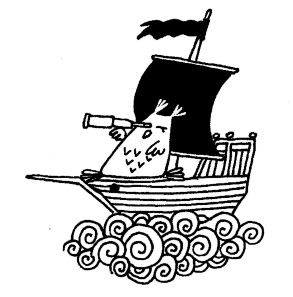
\includegraphics[scale=0.5]{22}}
\end{figure}
\end{SBSection*}

\end{song}

%\twocolumn
\begin{song}{Ленинградская (Все расстояния)}{}{Песни у костра}{Песни у костра}{}{}

\Ch{Am}{Все} расстоянья когда-нибудь в круг замы\Ch{E}{ка}ются,\par
\Ch{E}{Все} из разлук обязательно \Ch{E7}{встре}чей кон\Ch{Am}{ча}ются;\par
Должны про\Ch{Dm}{плыть} вокруг Зем\Ch{G}{ли,}\par
Вернуться в \Ch{C}{га}вань кораб\Ch{F}{ли,}\par   
Все поез\Ch{Dm}{да} в свои вер\Ch{E}{нуть}ся горо\Ch{Am}{да.}\\
 
Шумный вокзал то встречает друзей , то прощается,\par
Мы расстаемся, но снова назад возвращаемся -\par
Чтоб снова встать в огромный круг,\par
И снова знать, что рядом друг ,\par
И песни петь, чтоб больше не было разлук.\\
 
Все расстоянья когда-нибудь в круг замыкаются,\par
Все из разлук обязательно встречей кончаются;\par
И через год, и через пять,\par
Мы с вами встретимся опять,\par
Ничто не сможет нашей дружбе помешать.\par

\end{song}

%\twocolumn
\begin{song}{Десять капель}{}{Танцы Минус}{Танцы Минус}{}{}

Проигрыш: (2 раза)\par 
\Ch{C}{} \Ch{E}{} \Ch{Am}{} \Ch{F}{} \Ch{C}{} \Ch{E}{} \Ch{Am}{} \Ch{F}{}

\Ch{C}{Де}сять капель дож\Ch{E}{дя} у тебя на пле\Ch{Am}{че}\par
Ты забыла свой \Ch{F}{зонт,} ты спешила ко \Ch{C}{мне.}\par
Десять капель дож\Ch{E}{дя} на плече у те\Ch{Am}{бя,}\par
Десять капель люб\Ch{F}{ви,} десять капель ог\Ch{C}{ня}\\

Припев:\\(Три первых слова в припеве дублируются вторым голосом)\par
\tt\Ch{C}{Т}воя\Ch{E}{} ладо\Ch{Am}{нь} горит\Ch{F}{} в моих руках\par
\tt\Ch{C}{Л}юбви\Ch{E}{ }пож\Ch{Am}{ар} горит в тво\Ch{F}{их} глазах\\

Проигрыш.\\

Время делает шаг, время делает круг\par
Мы забудем друзей, мы забудем подруг\par
Просто выпьем вина из любви и огня\par
Десять капель меня, десять капель тебя\\

Припев.\\

Голос твой в тишине околдует меня\par
Ярким жарким огнем стану я до утра\par
Ты прикажешь гори, и я вспыхну любя\par
В этом пламени ты, в этом пламени я.\par

\end{song}

%\twocolumn
\begin{song}{Макет}{}{Песни у костра}{Сказка}{}{}
sadfsfthanks,\par
\begin{SBOpGroup}
asdas\
\end{SBOpGroup}
\begin{SBSection*}fdf\end{SBSection*}
\begin{SBVerse*}\end{SBVerse*}
\begin{SBChorus*}\end{SBChorus*}

\begin{SBOccurs}{23}
dsf
\end{SBOccurs}

\begin{SBSection*}
\begin{figure}[b!]
\center{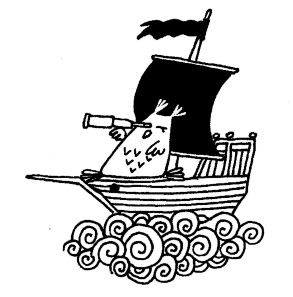
\includegraphics[scale=0.5]{22}}
\end{figure}
\end{SBSection*}
\end{song}

\mainmatter

\renewcommand{\footrulewidth}{0.0pt}
\renewcommand{\item}{\par\hangindent=40pt}
\renewcommand{\subitem}{\par\hangindent=40pt \hspace*{20pt}}
\renewcommand{\subsubitem}{\par\hangindent=40pt \hspace*{30pt}}

\newpage
\raggedright\input{/home/p_a/git/ska3ka/ps.adx}

\centering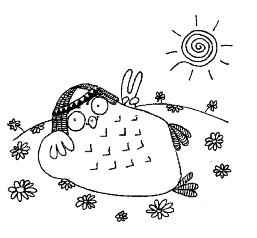
\includegraphics[scale=0.5]{10}

\newpage
\raggedright\input{/home/p_a/git/ska3ka/ps.tdx}

\centering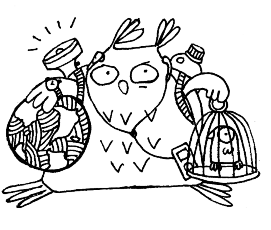
\includegraphics[scale=0.5]{11}

\end{document}


\centering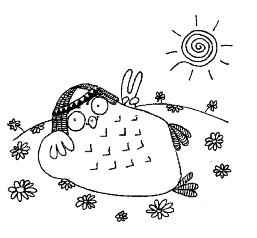
\includegraphics[scale=0.5]{10}

\newpage
\raggedright%\documentclass[a5paper,11pt]{book}
%\usepackage{fancyhdr}
%\usepackage[chordbk]{songbook}
%
%\usepackage[T2A]{fontenc}
%\usepackage[utf8]{inputenc}
%\usepackage[russian]{babel}
%
%\title{A Church Songbook}
%\author{}
%\date{Revised:  \RevDate}
%
%\newcommand{\RelDate}{13 November'19}
%\newcommand{\RevDate}{\today}

\documentclass[11pt,a5paper]{book}
\usepackage[a5paper]{geometry}
\usepackage[chordbk]{songbook}
\usepackage[T2A]{fontenc}
\usepackage[utf8]{inputenc}
\usepackage[russian]{babel}
\usepackage{cmap} % для работы поиска кириллицы в pdf

%\usepackage{amsmath,amsthm,amssymb}
%\usepackage{mathtext}


\usepackage[pdftex]{graphicx}
\usepackage{lscape}
%\usepackage{vmargin}
\usepackage{textcomp}
\usepackage{setspace}
%\usepackage{marvosym}
\usepackage{gensymb} %%%for \micro tag
\usepackage{upgreek} %%% \upmu
\usepackage{tipa}
\usepackage{phonetic}
%\usepackage[greek,english]{babel}
\usepackage{threeparttable}
\usepackage{multirow}
\usepackage{harvard}
\usepackage{longtable}
\renewcommand{\sectionmark}[1]{\markright{#1}}
\renewcommand{\chaptermark}[1]{\markboth{#1}{}}
\addto\captionsenglish{\renewcommand{\bibname}{References}}
\usepackage{latexsym,fancyhdr}

\newcommand{\RelDate}{26 Апреля'1984}
\newcommand{\RevDate}{\today}

%%%
% C.C.L.I. license number definition; for copyright licensing info.
% One of these macros will be manually inserted into the {CpyRt}
% parameter of the {song} environment.
%
%       \CCLInumber - The actual copyright license number.  Don't
%               insert this command in the {CpyRt} parameter, use one
%               of the others.
%       \CCLIed - Indicates a song falls under our CCLI license.
%       \NotCCLIed - Indicates a song doesn't fall under our CCLI
%               license.  Public Domain songs fall into this category.
%       \PGranted - We have received specific permission from the
%               copyright holder to use this song.
%       \PPending - We are in the process of obtaining permission to
%               use this song.
%%%
\newcommand{\CCLInumber}{Your CCLI Number}
\newcommand{\CCLIed}{{\CpyRtInfoFont (CCLI \CCLInumber)}}
\newcommand{\NotCCLIed}{\relax}
\newcommand{\PGranted}{\relax}
\newcommand{\PPending}{{\CpyRtInfoFont (Permission Pending)}}

%%%
% Title page information.
%%%
\title{ Сказочный песенник}
\author{}
\date{Созданно:  \RevDate}


%%%
% Define fonts to use in the headers and footers of the songbook.
%%%
\newcommand{\LHeadFont}{\normalsize}            % = cmr12  at 12pt
\newcommand{\CHeadFont}{\normalsize\rm}         % = cmr12  at 12pt
\newcommand{\RHeadFont}{\normalsize}            % = cmr12  at 12pt
\newcommand{\LFootFont}{\scriptsize}            % = cmr8   at  8pt
\newcommand{\CFootFont}{\tiny\myTinySF}         % = cmss8  at  8pt
\newcommand{\RFootFont}{\scriptsize}            % = cmr8   at  8pt

%%%
% Turn on and define fancy page heading/footing definition.
%%%
\pagestyle{fancy}

\ifChordBk
  % It's a words & chords songbook...
%  \addtolength{\headwidth}{\marginparsep}
%  \addtolength{\headwidth}{\marginparwidth}
  \renewcommand{\headrulewidth}{0.0pt}
  \renewcommand{\footrulewidth}{0.0pt}
%  \fancyhead[LE,RO]{\LHeadFont\emph{\leftmark\/}}
%  \fancyhead[CE,CO]{\CHeadFont\thepage}
  \fancyhead[RE,LO]{~}
\else\ifOverhead
  % It's an overhead...
  \renewcommand{\footrulewidth}{0pt}
  \renewcommand{\headrulewidth}{0pt}
  \fancyhead[LE,RO]{}
  \fancyhead[CE,CO]{}
  \fancyhead[RE,LO]{}
\else\ifWordBk
  % It's a words only songbook...
  \addtolength{\headwidth}{\marginparsep}
  \addtolength{\headwidth}{\marginparwidth}
  \renewcommand{\headrulewidth}{0.0pt}
  \renewcommand{\footrulewidth}{0.0pt}
  \fancyhead[LE,RO]{\LHeadFont A Church Songbook}
  \fancyhead[CE,CO]{\CHeadFont\thepage}
  \fancyhead[RE,LO]{\RHeadFont\RelDate}
\fi\fi\fi

%\fancyfoot[LE,RO]{\LFootFont Property of The Church}
%\ifSongEject
%  \fancyfoot[CE,CO]{\CFootFont \RevDate}
%\else
%  \fancyfoot[CE,CO]{\CFootFont}
%\fi
%\fancyfoot[RE,LO]{\RFootFont Material used by permission.}

%%%
% Turn on/off index-file generation.  Uncomment the \makeindex line to
% turn index generation on;  comment it out to turn index generation
% off.
%%%
\makeTitleIndex         %% Title and First Line Index.
\makeTitleContents      %% Table of Contents.
\makeKeyIndex           %% Index of song by key.
\graphicspath{{img/}} % папка с картинками
\DeclareGraphicsExtensions{.pdf,.png,.jpg} % форматы, которые будем считать картинками

%\newenvironment{song}[7][Y]{
%% Comment markers to negate
%\if#1Y\ExcludeSongfalse\else\ExcludeSongtrue\fi% the newline.
%\ifPrintAllSongs\ExcludeSongfalse\fi
%\SongMarkboth{\relax}{\relax}
%\SBinSongEnvtrue
%\renewcommand{\SBinSongEnv}{\True}
%\ifWordsOnly
%	\setlength{\parindent}{0pt}
%\fi

%%%
% Redefine fonts from SongBook style that I don't like.
%%%
\font\myTinySF=cmss8 at 8pt
\renewcommand{\CpyRtInfoFont}{\tiny\myTinySF}


%
%\font\myTinySF=cmss8    at  8pt
%\font\myHugeSF=cmssbx10 at 25pt
%\renewcommand{\CpyRtInfoFont}{\tiny\myTinySF}
%\newcommand{\myTitleFont}{\Huge\myHugeSF}
%\newcommand{\mySubTitleFont}{\large\sf}

%%% Работа с русским языком
%\usepackage[no-math]{fontspec}      %% подготавливает загрузку шрифтов Open Type, True Type и др.
%\defaultfontfeatures{Ligatures={TeX},Renderer=Basic}  %% свойства шрифтов по умолчанию
%\setmainfont[Ligatures={TeX,Historic}]{Times New Roman} %% задаёт основной шрифт документа
%\setsansfont{Helvetica Neue}                    %% задаёт шрифт без засечек

%\newfontfamily{\allods}{AllodsWest}

\newcommand{\SBPubDomm}{~}
\renewcommand{\CpyRt}[3][Y]{%
\if#1Y\begin{center}\fi
\if\blank{#2}%
\if\blank{#3}%
{\CpyRtFont\copyright \SBUnknownTag{} \CpyRtInfoFont}%
\else
{\CpyRtFont\copyright \SBUnknownTag{} \CpyRtInfoFont #3}%
\fi%
\else%
\ifthenelse{\equal{#2}{\SBPubDomm}}
{%then
{\CpyRtFont #2 \CpyRtInfoFont #3}%
}{%else
{\CpyRtFont #2 \CpyRtInfoFont #3}%
}%fi
\fi%
\if#1Y\end{center}\fi
}


\newcommand{\SBUnknownTagg}{~}
\renewcommand{\WAndM}[2][Y]{~}
\renewcommand{\WAndM}[2][Y]{%
\if#1Y\begin{center}\fi
\if\blank{#2}%
{\SBUnknownTagg}%
\else
{~}%
\fi
\if#1Y\end{center}\fi
}

\renewcommand{\STitle}[3][Y]{%
\setcounter{SBVerseCnt}{0}%
\setcounter{SBSectionCnt}{0}%
\ifExcludeSong\relax%
	\else\keyIndex{{\protect\sbChord#3\protect\relax} -- #2}{\theSBSongCnt}\fi%
	\vspace{\SpaceAboveSTitle}%
\if#1Y\begin{center}\fi
	{}{\STitleFont\LARGE #2}%
	\ifWordsOnly\relax\else\fi%
	\if#1Y\end{center}\fi
\STitleMarkboth{#2}{\relax}%
}


%\renewenvironment{SBOpGroup}{%
%	\sbSetsbBaselineSkipAmt%
%	\bgroup%
%	\begin{list}{\hbox{}}
%	  {\setlength {\leftmargin}
%		{\HangAmt}
%		\setlength{\itemindent}
%			{-\HangAmt}
%		\setlength{\listparindent}{-\HangAmt}
%		\setlength{\topsep}{0pt}
%		\setlength{\parsep}{0pt}
%		\setlength{\labelwidth}{0pt}
%		\setlength{\labelsep}{0pt}
%		\setlength{\baselineskip} {\sbBaselineSkipAmt}
%	}%\item}
%{\end{list}%
\newcommand{\SBChorusTagg}{Припев}
\renewenvironment{SBChorus}{%
\sbSetsbBaselineSkipAmt%
\bgroup%
\SBChorusMarkright{\SBChorusTag}
\begin{list}{{\SBChorusTagFont\SBChorusTagg}}
{\setlength {\leftmargin}
{\LeftMarginSBChorus + \HangAmt}
\setlength{\itemindent}
{-\HangAmt}
\setlength{\listparindent}{-\HangAmt}
\setlength{\parsep}
{0pt}
\setlength{\baselineskip} {\sbBaselineSkipAmt}
}%
\item}
{\end{list}%
\egroup%
\SpaceAfterChorus%
}

\renewcommand{\tt}{\indent \indent}
%\renewcommand{\nt}{\noindent}


\usepackage{amsmath}

\makeArtistIndex
\makeTitleIndex         %% Title and First Line Index.
\makeTitleContents      %% Table of Contents.
\makeKeyIndex           %% Index of song by key.
%\usepackage{printallsongs}

\begin{document} 
\maketitle

\mainmatter


\begin{song}{Вожатский гимн}{}{Сказка}{Сказка}{}{}

По \Ch{Am}{ла}герю подъём, нас горн зовёт!\par
Забудь о том, что ночь была бес\Ch{C}{сон}ною\par
Смо\Ch{Dm}{чи} водою \Ch{G}{ве}ки воспа\Ch{C}{лён}\Ch{F}{ные}\par    
По\Ch{Dm}{вя}зывай свой \Ch{E}{галс}тук — и впе\Ch{Am (A7)}{рёд!}\par
Смо\Ch{Dm}{чи} водою \Ch{G}{ве}ки воспа\Ch{C}{лён}\Ch{F}{ные}\par    
По\Ch{Dm}{вя}зывай свой \Ch{E}{галс}тук — и впе\Ch{Am (A7)}{рёд!}\par

%	\begin{SBChorus*}
\ttНе\Ch{E}{про}сто воспитывать \Ch{Am}{но}вых людей,\par
\ttНу \Ch{E}{что} ж, это наша с то\Ch{Am}{бою} свя\Ch{A7}{ты}ня.\par
\ttМой \Ch{Dm}{друг}, нам до\Ch{G}{ве}рили \Ch{C}{ду}ши де\Ch{F}{тей},\par
\ttИх \Ch{Dm}{ра}достный \Ch{Am}{смех} нам на\Ch{E}{гра}да от\Ch{Am}{ны}не.\par
\ttМой \Ch{Dm}{друг}, нам до\Ch{G}{ве}рили \Ch{C}{ду}ши де\Ch{F}{тей},\par
\ttИх \Ch{Dm}{ра}достный \Ch{Am}{смех} нам на\Ch{E}{гра}да от\Ch{Am}{ны}не.\\
%\end{SBChorus*}

Отбой, засыпает детвора.\par
Взгляни на их улыбки полусонные,\par
Пускай им снятся острова зелёные,\par
А нам опять работать до утра!\par
Пускай им снятся острова зелёные,\par
А нам опять работать до утра!\par

\tt И пусть от бессилья затихнешь не раз,\par
\ttИ голос усталый до хрипа натружен,\par
\ttПусть будут умней и счастливее нас\par
\ttТе дети, в которых вложили мы души!\par
\ttПусть будут умней и счастливее нас\par
\ttТе дети, в которых вложили мы души!

\end{song}

\begin{song}{Сказка в неглиже}{}{Сказка}{Сказка}{}{}

Есть у \Ch{C}{каж}дого добрая сказка в ду\Ch{F}{ше,}\par 
Надо \Ch{G}{толь}ко прочесть этой сказки стра\Ch{C}{ни}цы.\par
В тиши\Ch{C}{не}, разо\Ch{C7}{де}тая вся в негли\Ch{F}{же,}\par
Пусть на\Ch{G}{ве}ки она, пусть на\Ch{F}{ве}ки она сохра\Ch{C}{ни}тся. \Ch{C7}{ }\par 
В тиши\Ch{F}{не,} разо\Ch{G}{де}тая вся в негли\Ch{C}{же,} \Ch{Am}{}\par
Пусть на\Ch{F}{ве}ки она, пусть на\Ch{G}{ве}ки она сохра\Ch{C}{ни}тся.\\


\ttЭту сказку пред другом раскрыть поспеши,\par
\ttА врагу не спеши эту сказку поведать.\par
\ttПусть растут и читают ее малыши.\par
\ttБудь добрей, и тебя минут всякие беды.\par
\ttПусть растут и читают ее малыши.\par
\ttБудь добрей, и тебя минут всякие беды.\\


\Ch{C7}{}Будет \Ch{F}{мно}го распутий, \Ch{G}{до}рог и тре\Ch{C}{вог.}\Ch{Am}{}\par
На вис\Ch{F}{ки} твои ляжет \Ch{G}{не}тающий \Ch{C}{ин}ей, \Ch{C7}{}\par
И пой\Ch{F}{мёшь,} научившись чи\Ch{G}{тать} между \Ch{C}{строк:} \Ch{Am}{}\par
Даже \Ch{F}{гнус}ный злодей \Ch{G}{в} этой сказке не\Ch{C}{ви}нен. \Ch{C7}{}\par
И пой\Ch{F}{мёшь,} научившись чи\Ch{G}{тать} между ст\Ch{C}{рок:} \Ch{A}{}\par
Даже \Ch{F}{гнус}ный злодей \Ch{G}{в} этой сказке не\Ch{C}{ви}нен.\\

\Ch{C}{} \Ch{G}{} \Ch{F}{} \Ch{G}{} \Ch{C}{} \Ch{C7}{}\par
\Ch{C}{} \Ch{G}{} \Ch{F}{} \Ch{G}{} \Ch{C}{}
\end{song}

%\twocolumn
\begin{song}{Вожатский марш}{}{Сказка}{Сказка}{}{}

Есть на\Ch{Am}{род} у нас весёлый,\par
Самой \Ch{C}{луч}шей в мире пробы,\par
Песни \Ch{G}{петь} всегда мас\Ch{C}{так.}\Ch{A7}{}\par
Он всег\Ch{Dm}{да} всего добьётся,\par
Он Вожа\Ch{Am}{ты}ми зовётся,\par
\Ch{E}{Так} и только \Ch{Am (A7)}{так!}\par
Он всег\Ch{Dm}{да} всего добьётся,\par
Он Во\Ch{Am}{жа}тыми зовётся,\par
\Ch{E}{Так} и только \Ch{Am (A7)}{так!}\\

Домосед привязан к дому\par
И по случаю такому,\par
Он из дома — ни на шаг!\par
А вожатый — он в дороге,\par
Он готов в огонь и в воду,\par
Так и только так!\par
А вожатый — он в дороге,\par
Он готов в огонь и в воду,\par
Так и только так!\\
\newpage
Жадный денежки считает,\par
Все считает и считает,\par
К пятаку кладет пятак.\par
А вожатый деньги тратит,\par
Не боясь, что их не хватит,\par
Так и только так!\par
А вожатый деньги тратит,\par
Не боясь, что их не хватит,\par
Так и только так!\\

Холостяк в любовь не верит,\par
Все не верит и не верит,\par
Потому что холостяк.\par
А вожатых не влюблённых\par
Не найдёшь определённо,\par
Так и только так!\par
А вожатых не влюблённых\par
Не найдёшь определённо,\par
Так и только так!\par

\begin{SBSection*}
\begin{figure}[b!]
\center{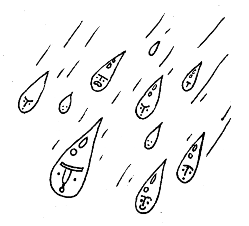
\includegraphics[scale=0.5]{16}}
\end{figure}
\end{SBSection*}
\end{song}

%\twocolumn
\begin{song}{Двадцать дней}{}{Сказка}{Сказка}{}{}


Двадцать дн\Ch{Dm}{ей} – это смена без дня.\par
“Маловато”,– вам скажут друзь\Ch{Gm}{я,}\par
А вожатый отв\Ch{C}{ет}ит люб\Ch{F}{ой}:\par
Это ср\Ch{Gm}{ок} очень д\Ch{A}{аж}е больш\Ch{Dm}{ой!}\\
 

Припев:\par
\ttМожно з\Ch{Gm C}{а-а-а-а} него усп\Ch{Dm}{ет}ь,\par
\ttНаприм\Ch{Gm}{ер,} полмилли\Ch{A}{он}а песен сп\Ch{Dm}{еть,}\par
\ttНо не к\Ch{Gm}{ажд}ый ведь поймет,\par
\ttКак так быстро раскрыв\Ch{A}{ат}ься может р\Ch{Dm}{от!}\\


Для полярника это не срок:\par
Не успеет просохнуть носок.\par
А вожатый успеет подряд \par
Вымыть, высушить сотню ребят!\\

Припев:\par
\ttВедь за смену, как за год \par
\ttСтолько разных мелочей произойдет,\par
\ttНо пока что нам везет,\par
\ttНас начальство для чего-то бережёт.\\


\newpage
Хоть и длинными кажутся дни,\par
Но как миг пролетели они.\par
Будешь долго потом вспоминать,\par
Как в отбой ты любил слово «СПАААТЬ!!!»\\

Припев:\par
\tt          	— Говорят за двадцать дней \par
\tt          	Все узнаешь о напарнице своей…\par
\tt          	— Только это ерунда,\par
\tt          	Обо всем ты не узнаешь никогда!\\

Смена вряд ли даст ответ:\par
Ты нашел свое призванье или нет.\par
Так что надо продолжать,\par
Двадцать раз по двадцать суток отсчитать!\\

\begin{SBSection*}
\begin{figure}[b!]
\center{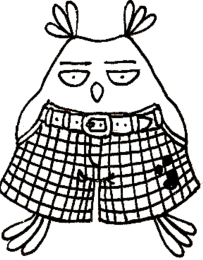
\includegraphics[scale=0.5]{17}}
\end{figure}
\end{SBSection*}

\end{song}

%\twocolumn
\begin{song}{Непогода}{}{Павел Смеян}{Павел Смеян}{}{}

\Ch{D}{Из}менения в природе \Ch{G}{пр}оисходят г\Ch{A}{од} от года,\par
\Ch{D}{Не}погода нынче в моде,\Ch{G}{} н\Ch{F#7}{епог}ода, непогода,\par
\Ch{}Hm{Слов}но из вод\Ch{F#7}{опро}вода \Ch{D7}{ль}ёт на нас с неб\Ch{G}{ес} во\Ch{Hm}{да…}\par
Полг\Ch{G}{од}а плох\Ch{A}{ая} пог\Ch{D}{од}а, \Ch{Hm}{пол}го\Ch{G}{да} — совс\Ch{A}{ем} нику\Ch{D}{да}.\par
Полг\Ch{G}{од}а плох\Ch{A}{ая} пог\Ch{D}{од}а, \Ch{Hm}{пол}го\Ch{G}{да} — сов\Ch{F#7}{сем} нику\Ch{Hm}{да.}\\


\SBChorusTagg:\par
\ttНикуда, нику\Ch{Em}{да н}ельз\Ch{A}{я} укр\Ch{D}{ы}ться н\Ch{Hm}{ам,}\par
\ttНо откладывать ж\Ch{Em}{изнь} ни\Ch{A}{как} нель\Ch{D}{зя}, \Ch{Hm}{}\par
\ttНикуда, нику\Ch{Em}{да, н}о зн\Ch{A}{ай}, что гд\Ch{D}{е}-то т\Ch{Hm}{ам}\par
\ttКто-то ищет теб\Ch{G}{я} сре\Ch{F#7}{ди д}ожд\Ch{Hm}{я.} \Ch{A}{}\\


Грома грозные раскаты от заката до восхода,\par
За грехи людские плата — непогода, непогода,\par
Не ангина, не простуда, посерьёзнее беда.\par
Полгода плохая погода, полгода — совсем никуда\par,
Полгода плохая погода, полгода — совсем никуда.\\\


\SBChorusTagg:\par
\ttНикуда, нику\Ch{Em}{да н}ельз\Ch{A}{я} укр\Ch{D}{ы}ться н\Ch{Hm}{ам,}\par
\ttНо откладывать ж\Ch{Em}{изнь} ни\Ch{A}{как} нель\Ch{D}{зя}, \Ch{Hm}{}\par
\ttНикуда, нику\Ch{Em}{да, н}о зн\Ch{A}{ай}, что гд\Ch{D}{е}-то т\Ch{Hm}{ам}\par
\ttКто-то ищет теб\Ch{G}{я} сре\Ch{F#7}{ди д}ожд\Ch{Hm}{я.} \Ch{A}{}\\


\end{song}

%\twocolumn
\begin{song}{Птенцы}{}{Сказка}{Сказка}{}{}

\Ch{Am}{}  \Ch{Am}{}

Как птенцы из гнез\Ch{Dm}{да} мы \Ch{E}{вы}па\Ch{Am}{ли.}\par
Ты не бойся при\Ch{Dm}{хо}да \Ch{G}{ве}че\Ch{C}{ра.}\par
Под та\Ch{A7}{ки}ми боль\Ch{F}{ши}ми \Ch{A7}{ли}па\Ch{Dm}{ми}\par
Нам с то\Ch{F}{бой} опа\Ch{Dm}{сать}ся \Ch{F}{не}\Ch{E}{че}\Ch{Am}{го.}\\
 
Под такими густыми звёздами -\par
Разве их не для нас рассыпали,\par
Мы не против гнездовья - просто мы\par
Из него ненароком выпали.\\

Это только вначале кажется,\par
Что без дома прожить нельзя никак,\par
Что важней пропитанья кашица,\par
Чем огромные звёзды на небе.\\

Ты не бойся ни тьмы, ни холода.\par
Будет день и найдётся пища нам,\par
Мы ещё пролетим над городом\par
На крыле до небес возвышенном.\\

Пролетим ещё - эка невидаль\par
Над Нью-Йорком, Парижем, Триполи\par
И над липой, откуда некогда,\par
Как птенцы из гнезда мы выпали.\\

Как птенцы из гнезда мы выпали.\par
Ты не бойся прихода вечера.\par
Под такими большими липами\par
Нам с тобой опасаться нечего.\\

\end{song}

%\twocolumn
\begin{song}{Продавец зонтиков}{}{Веня Дркин}{Веня Дркин}{}{}

\Ch{Am}{Город} этот выдумал о\Ch{Dm}{дин} художник,\par
\Ch{G}{Лю}ди в нем не знали, что та\Ch{C}{ко}е дождик.\par
\Ch{A7}{Про}сто не слыхали, что та\Ch{Dm}{ко}е зонтик –\par
\Ch{E7}{Вот} такие люди жили в \Ch{Am}{го}роде том.\par
И один чудак, в старый плащ одетый,\par
Продавал там зонтики зимой и летом,\par
Продавал там зонтики зимой и летом\par
И такую песенку он напевал:\\

\SBChorusTagg:\par
\tt“Господа, купите зонтик.\par
\ttБелый зонтик, красный зонтик,\par
\ttЖелтый зонтик, синий зонтик –\par
\ttМожет пригодится вам.”\\

Были домики у них из пластилина,\par
Из пустых коробочек автомашины,\par
И, не опасаясь никакой ангины,\par
Маленькие люди жили в городе том.\par
Маленькие были у людей заботы:\par
Шли они в кино или в театр с работы.\par
Вечером в подъезде целовался кто-то.\par
Все шутили и смеялись над стариком.\\


\SBChorusTagg.\\

\newpage

Маленькое небо как-то вдруг намокло,\par
В крошечных домишках задрожали стекла,\par
И огромный дождь пошел гулять по крышам,\par
Сразу все схватили насморк в городе том.\par
Вспомнили тут люди о торговце старом,\par
Кинулись искать его по всем базарам,\par
Но исчез торговец со своим товаром.\par
Только песенка осталась в память о нем:\\

\SBChorusTagg.\par

\begin{SBSection*}
\begin{figure}[b!]
\center{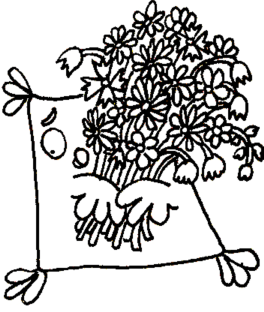
\includegraphics[scale=0.5]{15}}
\end{figure}
\end{SBSection*}

\end{song}

%\twocolumn
\begin{song}{Белая гвардия}{}{Белая гвардия}{Белая гвардия}{}{}

Проигрыш: (2 раза)\par 
\Ch{Am}{} \Ch{D}{} \Ch{G}{} \Ch{C}{} \Ch{Am}{} \Ch{H7}{} \Ch{Em}\\

\Ch{Em}{Белая} гвардия, белый снег,\par
\Ch{Am7}{Белая} музыка революций.\par
\Ch{D7}{Белая} женщина, нервный смех,\par
\Ch{G}{Белого} платья слегка коснуться.\par
 
Белой рукой распахнуть окно,\par
Белого света в нем не видя.\par
Белое выпить до дна вино,\par
В красную улицу в белом выйти.\\

Припев:\par
\ttКог\Ch{Em}{да} ты вернешься,\par
\ttВсе будет и\Ch{Am}{на}че, и нам бы узнать друг друга,\par
\ttКог\Ch{D7}{да} ты вернешься,\par
\ttА я не же\Ch{G}{на} и даже \Ch{H7}{не} подруга.\par
\ttКог\Ch{C}{да} ты вернешься,\par
\ttКо мне, так без\Ch{Am}{ум}но тебя любившей в прошлом,\par
\tt\Ch{D7}{Ко}гда ты вернешься -\par
\ttУвидишь, что ж\Ch{G}{ре}бий давно и не \Ch{E7}{нами} брошен.\\

Проигрыш.\\
 
\newpage
Сизые сумерки прошлых лет\par
Робко крадутся по переулкам.\par
В этом окне еле брезжит свет,\par
Ноты истрепаны, звуки гулки.\par
Тонкие пальцы срывают аккорд...\par
Нам не простят безрассудного дара.\par
Бьются в решетку стальных ворот\par
Пять океанов земного шара.\\

Припев. \par
Проигрыш.\\
 
Красный трамвай простучал в ночи,\par
Красный закат догорел в бокале,\par
Красные-красные кумачи\par
С красных деревьев на землю упали.\par
Я не ждала тебя в октябре,\par
Виделись сны, я листала сонник:\par
Красные лошади на заре\par
Били копытами о подоконник.\\

Припев:\par
\ttКогда ты вернешься,\par
\ttВсе будет иначе, и нам бы узнать друг друга,\par
\ttКогда ты вернешься,\par
\ttА я не жена и даже не подруга.\par
\ttКогда ты вернешься,\par
\ttВернешься в наш город обетованный,\par
\ttКогда ты вернешься -\par
\ttТакой невозможный и такой желанный?\\

Проигрыш.\par

\end{song}

%\twocolumn
\begin{song}{Перевал}{}{Песни у костра}{Песни у костра}{}{}


\Ch{Am}{Про}сто нечего нам \Ch{Dm}{боль}ше терять\par
\Ch{E}{Всё} нам вспомнится на \Ch{Am}{Страшном} суде.\par
Эта ночь легла, как \Ch{Dm}{тот} перевал,\par
\Ch{G}{За} которым испол\Ch{C}{нень}е надежд.\par
\Ch{A7}{Про}сто прожитое—про\Ch{Dm}{жи}то зря, \Ch{G}{}\par
Но не в этом, пони\Ch{C}{мае}шь ли, соль… \Ch{Am}{}\par
Слышишь, падают дож\Ch{Dm}{ди} октября.\par
\Ch{E}{Ви}дишь, старый дом сто\Ch{Am}{ит} средь лесов.\\

Мы затопим в доме печь, в доме печь,\par
Мы гитару позовем со стены.\par
Просто нечего нам больше беречь,\par
Ведь за нами все мосты сожжены.\par
Все мосты, все перекрёстки дорог,\par
Все прошёптанные тайны в ночи.\par
Каждый сделал все, что смог, все, что смог,\par
Мы об этом помолчим, помолчим.\\


И луна взойдет заплывшей свечой,\par
Ставни скрипнут  на ветру, на ветру.\par
Ах, как я тебя люблю горячо,\par
Это годы не сотрут, не сотрут.\par
Мы оставшихся друзей соберем,\par
Мы набьем картошкой старый рюкзак,\par
Люди спросят: "Что за шум, что за гам?"\par
Мы ответим: "Просто так,  просто так”...\\

\newpage

    Просто так идут дожди в октябре,\par
    И потеряны от счастья ключи.\par
    Это всё, конечно, мне, конечно, мне,\par
    Но об этом помолчим, помолчим.\par
    Просто прожитое—прожито зря,\par
    Но не в этом, понимаешь ли, соль…\par
    Слышишь, падают дожди октября.\par
    Видишь, старый дом стоит средь лесов.\par


\begin{SBSection*}
\begin{figure}[b!]
\center{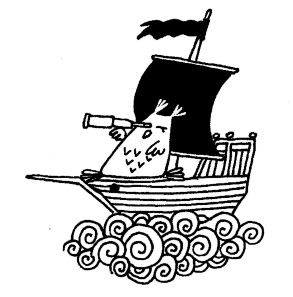
\includegraphics[scale=0.5]{22}}
\end{figure}
\end{SBSection*}

\end{song}

%\twocolumn
\begin{song}{Ленинградская (Все расстояния)}{}{Песни у костра}{Песни у костра}{}{}

\Ch{Am}{Все} расстоянья когда-нибудь в круг замы\Ch{E}{ка}ются,\par
\Ch{E}{Все} из разлук обязательно \Ch{E7}{встре}чей кон\Ch{Am}{ча}ются;\par
Должны про\Ch{Dm}{плыть} вокруг Зем\Ch{G}{ли,}\par
Вернуться в \Ch{C}{га}вань кораб\Ch{F}{ли,}\par   
Все поез\Ch{Dm}{да} в свои вер\Ch{E}{нуть}ся горо\Ch{Am}{да.}\\
 
Шумный вокзал то встречает друзей , то прощается,\par
Мы расстаемся, но снова назад возвращаемся -\par
Чтоб снова встать в огромный круг,\par
И снова знать, что рядом друг ,\par
И песни петь, чтоб больше не было разлук.\\
 
Все расстоянья когда-нибудь в круг замыкаются,\par
Все из разлук обязательно встречей кончаются;\par
И через год, и через пять,\par
Мы с вами встретимся опять,\par
Ничто не сможет нашей дружбе помешать.\par

\end{song}

%\twocolumn
\begin{song}{Десять капель}{}{Танцы Минус}{Танцы Минус}{}{}

Проигрыш: (2 раза)\par 
\Ch{C}{} \Ch{E}{} \Ch{Am}{} \Ch{F}{} \Ch{C}{} \Ch{E}{} \Ch{Am}{} \Ch{F}{}

\Ch{C}{Де}сять капель дож\Ch{E}{дя} у тебя на пле\Ch{Am}{че}\par
Ты забыла свой \Ch{F}{зонт,} ты спешила ко \Ch{C}{мне.}\par
Десять капель дож\Ch{E}{дя} на плече у те\Ch{Am}{бя,}\par
Десять капель люб\Ch{F}{ви,} десять капель ог\Ch{C}{ня}\\

Припев:\\(Три первых слова в припеве дублируются вторым голосом)\par
\tt\Ch{C}{Т}воя\Ch{E}{} ладо\Ch{Am}{нь} горит\Ch{F}{} в моих руках\par
\tt\Ch{C}{Л}юбви\Ch{E}{ }пож\Ch{Am}{ар} горит в тво\Ch{F}{их} глазах\\

Проигрыш.\\

Время делает шаг, время делает круг\par
Мы забудем друзей, мы забудем подруг\par
Просто выпьем вина из любви и огня\par
Десять капель меня, десять капель тебя\\

Припев.\\

Голос твой в тишине околдует меня\par
Ярким жарким огнем стану я до утра\par
Ты прикажешь гори, и я вспыхну любя\par
В этом пламени ты, в этом пламени я.\par

\end{song}

%\twocolumn
\begin{song}{Макет}{}{Песни у костра}{Сказка}{}{}
sadfsfthanks,\par
\begin{SBOpGroup}
asdas\
\end{SBOpGroup}
\begin{SBSection*}fdf\end{SBSection*}
\begin{SBVerse*}\end{SBVerse*}
\begin{SBChorus*}\end{SBChorus*}

\begin{SBOccurs}{23}
dsf
\end{SBOccurs}

\begin{SBSection*}
\begin{figure}[b!]
\center{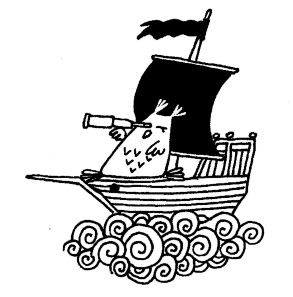
\includegraphics[scale=0.5]{22}}
\end{figure}
\end{SBSection*}
\end{song}

\mainmatter

\renewcommand{\footrulewidth}{0.0pt}
\renewcommand{\item}{\par\hangindent=40pt}
\renewcommand{\subitem}{\par\hangindent=40pt \hspace*{20pt}}
\renewcommand{\subsubitem}{\par\hangindent=40pt \hspace*{30pt}}

\newpage
\raggedright\input{/home/p_a/git/ska3ka/ps.adx}

\centering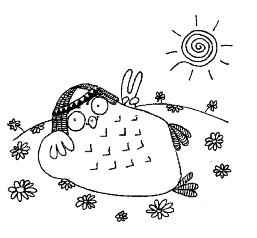
\includegraphics[scale=0.5]{10}

\newpage
\raggedright\input{/home/p_a/git/ska3ka/ps.tdx}

\centering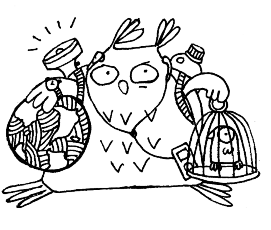
\includegraphics[scale=0.5]{11}

\end{document}


\centering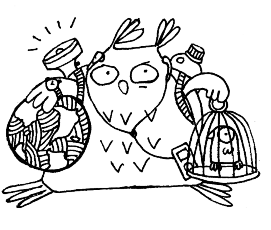
\includegraphics[scale=0.5]{11}

\end{document}


\centering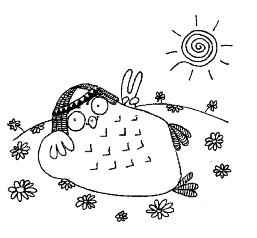
\includegraphics[scale=0.5]{10}

\newpage
\raggedright%\documentclass[a5paper,11pt]{book}
%\usepackage{fancyhdr}
%\usepackage[chordbk]{songbook}
%
%\usepackage[T2A]{fontenc}
%\usepackage[utf8]{inputenc}
%\usepackage[russian]{babel}
%
%\title{A Church Songbook}
%\author{}
%\date{Revised:  \RevDate}
%
%\newcommand{\RelDate}{13 November'19}
%\newcommand{\RevDate}{\today}

\documentclass[11pt,a5paper]{book}
\usepackage[a5paper]{geometry}
\usepackage[chordbk]{songbook}
\usepackage[T2A]{fontenc}
\usepackage[utf8]{inputenc}
\usepackage[russian]{babel}
\usepackage{cmap} % для работы поиска кириллицы в pdf

%\usepackage{amsmath,amsthm,amssymb}
%\usepackage{mathtext}


\usepackage[pdftex]{graphicx}
\usepackage{lscape}
%\usepackage{vmargin}
\usepackage{textcomp}
\usepackage{setspace}
%\usepackage{marvosym}
\usepackage{gensymb} %%%for \micro tag
\usepackage{upgreek} %%% \upmu
\usepackage{tipa}
\usepackage{phonetic}
%\usepackage[greek,english]{babel}
\usepackage{threeparttable}
\usepackage{multirow}
\usepackage{harvard}
\usepackage{longtable}
\renewcommand{\sectionmark}[1]{\markright{#1}}
\renewcommand{\chaptermark}[1]{\markboth{#1}{}}
\addto\captionsenglish{\renewcommand{\bibname}{References}}
\usepackage{latexsym,fancyhdr}

\newcommand{\RelDate}{26 Апреля'1984}
\newcommand{\RevDate}{\today}

%%%
% C.C.L.I. license number definition; for copyright licensing info.
% One of these macros will be manually inserted into the {CpyRt}
% parameter of the {song} environment.
%
%       \CCLInumber - The actual copyright license number.  Don't
%               insert this command in the {CpyRt} parameter, use one
%               of the others.
%       \CCLIed - Indicates a song falls under our CCLI license.
%       \NotCCLIed - Indicates a song doesn't fall under our CCLI
%               license.  Public Domain songs fall into this category.
%       \PGranted - We have received specific permission from the
%               copyright holder to use this song.
%       \PPending - We are in the process of obtaining permission to
%               use this song.
%%%
\newcommand{\CCLInumber}{Your CCLI Number}
\newcommand{\CCLIed}{{\CpyRtInfoFont (CCLI \CCLInumber)}}
\newcommand{\NotCCLIed}{\relax}
\newcommand{\PGranted}{\relax}
\newcommand{\PPending}{{\CpyRtInfoFont (Permission Pending)}}

%%%
% Title page information.
%%%
\title{ Сказочный песенник}
\author{}
\date{Созданно:  \RevDate}


%%%
% Define fonts to use in the headers and footers of the songbook.
%%%
\newcommand{\LHeadFont}{\normalsize}            % = cmr12  at 12pt
\newcommand{\CHeadFont}{\normalsize\rm}         % = cmr12  at 12pt
\newcommand{\RHeadFont}{\normalsize}            % = cmr12  at 12pt
\newcommand{\LFootFont}{\scriptsize}            % = cmr8   at  8pt
\newcommand{\CFootFont}{\tiny\myTinySF}         % = cmss8  at  8pt
\newcommand{\RFootFont}{\scriptsize}            % = cmr8   at  8pt

%%%
% Turn on and define fancy page heading/footing definition.
%%%
\pagestyle{fancy}

\ifChordBk
  % It's a words & chords songbook...
%  \addtolength{\headwidth}{\marginparsep}
%  \addtolength{\headwidth}{\marginparwidth}
  \renewcommand{\headrulewidth}{0.0pt}
  \renewcommand{\footrulewidth}{0.0pt}
%  \fancyhead[LE,RO]{\LHeadFont\emph{\leftmark\/}}
%  \fancyhead[CE,CO]{\CHeadFont\thepage}
  \fancyhead[RE,LO]{~}
\else\ifOverhead
  % It's an overhead...
  \renewcommand{\footrulewidth}{0pt}
  \renewcommand{\headrulewidth}{0pt}
  \fancyhead[LE,RO]{}
  \fancyhead[CE,CO]{}
  \fancyhead[RE,LO]{}
\else\ifWordBk
  % It's a words only songbook...
  \addtolength{\headwidth}{\marginparsep}
  \addtolength{\headwidth}{\marginparwidth}
  \renewcommand{\headrulewidth}{0.0pt}
  \renewcommand{\footrulewidth}{0.0pt}
  \fancyhead[LE,RO]{\LHeadFont A Church Songbook}
  \fancyhead[CE,CO]{\CHeadFont\thepage}
  \fancyhead[RE,LO]{\RHeadFont\RelDate}
\fi\fi\fi

%\fancyfoot[LE,RO]{\LFootFont Property of The Church}
%\ifSongEject
%  \fancyfoot[CE,CO]{\CFootFont \RevDate}
%\else
%  \fancyfoot[CE,CO]{\CFootFont}
%\fi
%\fancyfoot[RE,LO]{\RFootFont Material used by permission.}

%%%
% Turn on/off index-file generation.  Uncomment the \makeindex line to
% turn index generation on;  comment it out to turn index generation
% off.
%%%
\makeTitleIndex         %% Title and First Line Index.
\makeTitleContents      %% Table of Contents.
\makeKeyIndex           %% Index of song by key.
\graphicspath{{img/}} % папка с картинками
\DeclareGraphicsExtensions{.pdf,.png,.jpg} % форматы, которые будем считать картинками

%\newenvironment{song}[7][Y]{
%% Comment markers to negate
%\if#1Y\ExcludeSongfalse\else\ExcludeSongtrue\fi% the newline.
%\ifPrintAllSongs\ExcludeSongfalse\fi
%\SongMarkboth{\relax}{\relax}
%\SBinSongEnvtrue
%\renewcommand{\SBinSongEnv}{\True}
%\ifWordsOnly
%	\setlength{\parindent}{0pt}
%\fi

%%%
% Redefine fonts from SongBook style that I don't like.
%%%
\font\myTinySF=cmss8 at 8pt
\renewcommand{\CpyRtInfoFont}{\tiny\myTinySF}


%
%\font\myTinySF=cmss8    at  8pt
%\font\myHugeSF=cmssbx10 at 25pt
%\renewcommand{\CpyRtInfoFont}{\tiny\myTinySF}
%\newcommand{\myTitleFont}{\Huge\myHugeSF}
%\newcommand{\mySubTitleFont}{\large\sf}

%%% Работа с русским языком
%\usepackage[no-math]{fontspec}      %% подготавливает загрузку шрифтов Open Type, True Type и др.
%\defaultfontfeatures{Ligatures={TeX},Renderer=Basic}  %% свойства шрифтов по умолчанию
%\setmainfont[Ligatures={TeX,Historic}]{Times New Roman} %% задаёт основной шрифт документа
%\setsansfont{Helvetica Neue}                    %% задаёт шрифт без засечек

%\newfontfamily{\allods}{AllodsWest}

\newcommand{\SBPubDomm}{~}
\renewcommand{\CpyRt}[3][Y]{%
\if#1Y\begin{center}\fi
\if\blank{#2}%
\if\blank{#3}%
{\CpyRtFont\copyright \SBUnknownTag{} \CpyRtInfoFont}%
\else
{\CpyRtFont\copyright \SBUnknownTag{} \CpyRtInfoFont #3}%
\fi%
\else%
\ifthenelse{\equal{#2}{\SBPubDomm}}
{%then
{\CpyRtFont #2 \CpyRtInfoFont #3}%
}{%else
{\CpyRtFont #2 \CpyRtInfoFont #3}%
}%fi
\fi%
\if#1Y\end{center}\fi
}


\newcommand{\SBUnknownTagg}{~}
\renewcommand{\WAndM}[2][Y]{~}
\renewcommand{\WAndM}[2][Y]{%
\if#1Y\begin{center}\fi
\if\blank{#2}%
{\SBUnknownTagg}%
\else
{~}%
\fi
\if#1Y\end{center}\fi
}

\renewcommand{\STitle}[3][Y]{%
\setcounter{SBVerseCnt}{0}%
\setcounter{SBSectionCnt}{0}%
\ifExcludeSong\relax%
	\else\keyIndex{{\protect\sbChord#3\protect\relax} -- #2}{\theSBSongCnt}\fi%
	\vspace{\SpaceAboveSTitle}%
\if#1Y\begin{center}\fi
	{}{\STitleFont\LARGE #2}%
	\ifWordsOnly\relax\else\fi%
	\if#1Y\end{center}\fi
\STitleMarkboth{#2}{\relax}%
}


%\renewenvironment{SBOpGroup}{%
%	\sbSetsbBaselineSkipAmt%
%	\bgroup%
%	\begin{list}{\hbox{}}
%	  {\setlength {\leftmargin}
%		{\HangAmt}
%		\setlength{\itemindent}
%			{-\HangAmt}
%		\setlength{\listparindent}{-\HangAmt}
%		\setlength{\topsep}{0pt}
%		\setlength{\parsep}{0pt}
%		\setlength{\labelwidth}{0pt}
%		\setlength{\labelsep}{0pt}
%		\setlength{\baselineskip} {\sbBaselineSkipAmt}
%	}%\item}
%{\end{list}%
\newcommand{\SBChorusTagg}{Припев}
\renewenvironment{SBChorus}{%
\sbSetsbBaselineSkipAmt%
\bgroup%
\SBChorusMarkright{\SBChorusTag}
\begin{list}{{\SBChorusTagFont\SBChorusTagg}}
{\setlength {\leftmargin}
{\LeftMarginSBChorus + \HangAmt}
\setlength{\itemindent}
{-\HangAmt}
\setlength{\listparindent}{-\HangAmt}
\setlength{\parsep}
{0pt}
\setlength{\baselineskip} {\sbBaselineSkipAmt}
}%
\item}
{\end{list}%
\egroup%
\SpaceAfterChorus%
}

\renewcommand{\tt}{\indent \indent}
%\renewcommand{\nt}{\noindent}


\usepackage{amsmath}

\makeArtistIndex
\makeTitleIndex         %% Title and First Line Index.
\makeTitleContents      %% Table of Contents.
\makeKeyIndex           %% Index of song by key.
%\usepackage{printallsongs}

\begin{document} 
\maketitle

\mainmatter


\begin{song}{Вожатский гимн}{}{Сказка}{Сказка}{}{}

По \Ch{Am}{ла}герю подъём, нас горн зовёт!\par
Забудь о том, что ночь была бес\Ch{C}{сон}ною\par
Смо\Ch{Dm}{чи} водою \Ch{G}{ве}ки воспа\Ch{C}{лён}\Ch{F}{ные}\par    
По\Ch{Dm}{вя}зывай свой \Ch{E}{галс}тук — и впе\Ch{Am (A7)}{рёд!}\par
Смо\Ch{Dm}{чи} водою \Ch{G}{ве}ки воспа\Ch{C}{лён}\Ch{F}{ные}\par    
По\Ch{Dm}{вя}зывай свой \Ch{E}{галс}тук — и впе\Ch{Am (A7)}{рёд!}\par

%	\begin{SBChorus*}
\ttНе\Ch{E}{про}сто воспитывать \Ch{Am}{но}вых людей,\par
\ttНу \Ch{E}{что} ж, это наша с то\Ch{Am}{бою} свя\Ch{A7}{ты}ня.\par
\ttМой \Ch{Dm}{друг}, нам до\Ch{G}{ве}рили \Ch{C}{ду}ши де\Ch{F}{тей},\par
\ttИх \Ch{Dm}{ра}достный \Ch{Am}{смех} нам на\Ch{E}{гра}да от\Ch{Am}{ны}не.\par
\ttМой \Ch{Dm}{друг}, нам до\Ch{G}{ве}рили \Ch{C}{ду}ши де\Ch{F}{тей},\par
\ttИх \Ch{Dm}{ра}достный \Ch{Am}{смех} нам на\Ch{E}{гра}да от\Ch{Am}{ны}не.\\
%\end{SBChorus*}

Отбой, засыпает детвора.\par
Взгляни на их улыбки полусонные,\par
Пускай им снятся острова зелёные,\par
А нам опять работать до утра!\par
Пускай им снятся острова зелёные,\par
А нам опять работать до утра!\par

\tt И пусть от бессилья затихнешь не раз,\par
\ttИ голос усталый до хрипа натружен,\par
\ttПусть будут умней и счастливее нас\par
\ttТе дети, в которых вложили мы души!\par
\ttПусть будут умней и счастливее нас\par
\ttТе дети, в которых вложили мы души!

\end{song}

\begin{song}{Сказка в неглиже}{}{Сказка}{Сказка}{}{}

Есть у \Ch{C}{каж}дого добрая сказка в ду\Ch{F}{ше,}\par 
Надо \Ch{G}{толь}ко прочесть этой сказки стра\Ch{C}{ни}цы.\par
В тиши\Ch{C}{не}, разо\Ch{C7}{де}тая вся в негли\Ch{F}{же,}\par
Пусть на\Ch{G}{ве}ки она, пусть на\Ch{F}{ве}ки она сохра\Ch{C}{ни}тся. \Ch{C7}{ }\par 
В тиши\Ch{F}{не,} разо\Ch{G}{де}тая вся в негли\Ch{C}{же,} \Ch{Am}{}\par
Пусть на\Ch{F}{ве}ки она, пусть на\Ch{G}{ве}ки она сохра\Ch{C}{ни}тся.\\


\ttЭту сказку пред другом раскрыть поспеши,\par
\ttА врагу не спеши эту сказку поведать.\par
\ttПусть растут и читают ее малыши.\par
\ttБудь добрей, и тебя минут всякие беды.\par
\ttПусть растут и читают ее малыши.\par
\ttБудь добрей, и тебя минут всякие беды.\\


\Ch{C7}{}Будет \Ch{F}{мно}го распутий, \Ch{G}{до}рог и тре\Ch{C}{вог.}\Ch{Am}{}\par
На вис\Ch{F}{ки} твои ляжет \Ch{G}{не}тающий \Ch{C}{ин}ей, \Ch{C7}{}\par
И пой\Ch{F}{мёшь,} научившись чи\Ch{G}{тать} между \Ch{C}{строк:} \Ch{Am}{}\par
Даже \Ch{F}{гнус}ный злодей \Ch{G}{в} этой сказке не\Ch{C}{ви}нен. \Ch{C7}{}\par
И пой\Ch{F}{мёшь,} научившись чи\Ch{G}{тать} между ст\Ch{C}{рок:} \Ch{A}{}\par
Даже \Ch{F}{гнус}ный злодей \Ch{G}{в} этой сказке не\Ch{C}{ви}нен.\\

\Ch{C}{} \Ch{G}{} \Ch{F}{} \Ch{G}{} \Ch{C}{} \Ch{C7}{}\par
\Ch{C}{} \Ch{G}{} \Ch{F}{} \Ch{G}{} \Ch{C}{}
\end{song}

%\twocolumn
\begin{song}{Вожатский марш}{}{Сказка}{Сказка}{}{}

Есть на\Ch{Am}{род} у нас весёлый,\par
Самой \Ch{C}{луч}шей в мире пробы,\par
Песни \Ch{G}{петь} всегда мас\Ch{C}{так.}\Ch{A7}{}\par
Он всег\Ch{Dm}{да} всего добьётся,\par
Он Вожа\Ch{Am}{ты}ми зовётся,\par
\Ch{E}{Так} и только \Ch{Am (A7)}{так!}\par
Он всег\Ch{Dm}{да} всего добьётся,\par
Он Во\Ch{Am}{жа}тыми зовётся,\par
\Ch{E}{Так} и только \Ch{Am (A7)}{так!}\\

Домосед привязан к дому\par
И по случаю такому,\par
Он из дома — ни на шаг!\par
А вожатый — он в дороге,\par
Он готов в огонь и в воду,\par
Так и только так!\par
А вожатый — он в дороге,\par
Он готов в огонь и в воду,\par
Так и только так!\\
\newpage
Жадный денежки считает,\par
Все считает и считает,\par
К пятаку кладет пятак.\par
А вожатый деньги тратит,\par
Не боясь, что их не хватит,\par
Так и только так!\par
А вожатый деньги тратит,\par
Не боясь, что их не хватит,\par
Так и только так!\\

Холостяк в любовь не верит,\par
Все не верит и не верит,\par
Потому что холостяк.\par
А вожатых не влюблённых\par
Не найдёшь определённо,\par
Так и только так!\par
А вожатых не влюблённых\par
Не найдёшь определённо,\par
Так и только так!\par

\begin{SBSection*}
\begin{figure}[b!]
\center{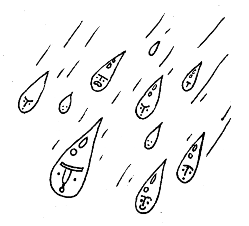
\includegraphics[scale=0.5]{16}}
\end{figure}
\end{SBSection*}
\end{song}

%\twocolumn
\begin{song}{Двадцать дней}{}{Сказка}{Сказка}{}{}


Двадцать дн\Ch{Dm}{ей} – это смена без дня.\par
“Маловато”,– вам скажут друзь\Ch{Gm}{я,}\par
А вожатый отв\Ch{C}{ет}ит люб\Ch{F}{ой}:\par
Это ср\Ch{Gm}{ок} очень д\Ch{A}{аж}е больш\Ch{Dm}{ой!}\\
 

Припев:\par
\ttМожно з\Ch{Gm C}{а-а-а-а} него усп\Ch{Dm}{ет}ь,\par
\ttНаприм\Ch{Gm}{ер,} полмилли\Ch{A}{он}а песен сп\Ch{Dm}{еть,}\par
\ttНо не к\Ch{Gm}{ажд}ый ведь поймет,\par
\ttКак так быстро раскрыв\Ch{A}{ат}ься может р\Ch{Dm}{от!}\\


Для полярника это не срок:\par
Не успеет просохнуть носок.\par
А вожатый успеет подряд \par
Вымыть, высушить сотню ребят!\\

Припев:\par
\ttВедь за смену, как за год \par
\ttСтолько разных мелочей произойдет,\par
\ttНо пока что нам везет,\par
\ttНас начальство для чего-то бережёт.\\


\newpage
Хоть и длинными кажутся дни,\par
Но как миг пролетели они.\par
Будешь долго потом вспоминать,\par
Как в отбой ты любил слово «СПАААТЬ!!!»\\

Припев:\par
\tt          	— Говорят за двадцать дней \par
\tt          	Все узнаешь о напарнице своей…\par
\tt          	— Только это ерунда,\par
\tt          	Обо всем ты не узнаешь никогда!\\

Смена вряд ли даст ответ:\par
Ты нашел свое призванье или нет.\par
Так что надо продолжать,\par
Двадцать раз по двадцать суток отсчитать!\\

\begin{SBSection*}
\begin{figure}[b!]
\center{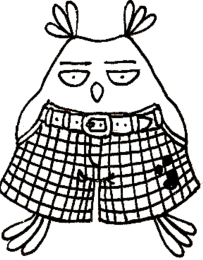
\includegraphics[scale=0.5]{17}}
\end{figure}
\end{SBSection*}

\end{song}

%\twocolumn
\begin{song}{Непогода}{}{Павел Смеян}{Павел Смеян}{}{}

\Ch{D}{Из}менения в природе \Ch{G}{пр}оисходят г\Ch{A}{од} от года,\par
\Ch{D}{Не}погода нынче в моде,\Ch{G}{} н\Ch{F#7}{епог}ода, непогода,\par
\Ch{}Hm{Слов}но из вод\Ch{F#7}{опро}вода \Ch{D7}{ль}ёт на нас с неб\Ch{G}{ес} во\Ch{Hm}{да…}\par
Полг\Ch{G}{од}а плох\Ch{A}{ая} пог\Ch{D}{од}а, \Ch{Hm}{пол}го\Ch{G}{да} — совс\Ch{A}{ем} нику\Ch{D}{да}.\par
Полг\Ch{G}{од}а плох\Ch{A}{ая} пог\Ch{D}{од}а, \Ch{Hm}{пол}го\Ch{G}{да} — сов\Ch{F#7}{сем} нику\Ch{Hm}{да.}\\


\SBChorusTagg:\par
\ttНикуда, нику\Ch{Em}{да н}ельз\Ch{A}{я} укр\Ch{D}{ы}ться н\Ch{Hm}{ам,}\par
\ttНо откладывать ж\Ch{Em}{изнь} ни\Ch{A}{как} нель\Ch{D}{зя}, \Ch{Hm}{}\par
\ttНикуда, нику\Ch{Em}{да, н}о зн\Ch{A}{ай}, что гд\Ch{D}{е}-то т\Ch{Hm}{ам}\par
\ttКто-то ищет теб\Ch{G}{я} сре\Ch{F#7}{ди д}ожд\Ch{Hm}{я.} \Ch{A}{}\\


Грома грозные раскаты от заката до восхода,\par
За грехи людские плата — непогода, непогода,\par
Не ангина, не простуда, посерьёзнее беда.\par
Полгода плохая погода, полгода — совсем никуда\par,
Полгода плохая погода, полгода — совсем никуда.\\\


\SBChorusTagg:\par
\ttНикуда, нику\Ch{Em}{да н}ельз\Ch{A}{я} укр\Ch{D}{ы}ться н\Ch{Hm}{ам,}\par
\ttНо откладывать ж\Ch{Em}{изнь} ни\Ch{A}{как} нель\Ch{D}{зя}, \Ch{Hm}{}\par
\ttНикуда, нику\Ch{Em}{да, н}о зн\Ch{A}{ай}, что гд\Ch{D}{е}-то т\Ch{Hm}{ам}\par
\ttКто-то ищет теб\Ch{G}{я} сре\Ch{F#7}{ди д}ожд\Ch{Hm}{я.} \Ch{A}{}\\


\end{song}

%\twocolumn
\begin{song}{Птенцы}{}{Сказка}{Сказка}{}{}

\Ch{Am}{}  \Ch{Am}{}

Как птенцы из гнез\Ch{Dm}{да} мы \Ch{E}{вы}па\Ch{Am}{ли.}\par
Ты не бойся при\Ch{Dm}{хо}да \Ch{G}{ве}че\Ch{C}{ра.}\par
Под та\Ch{A7}{ки}ми боль\Ch{F}{ши}ми \Ch{A7}{ли}па\Ch{Dm}{ми}\par
Нам с то\Ch{F}{бой} опа\Ch{Dm}{сать}ся \Ch{F}{не}\Ch{E}{че}\Ch{Am}{го.}\\
 
Под такими густыми звёздами -\par
Разве их не для нас рассыпали,\par
Мы не против гнездовья - просто мы\par
Из него ненароком выпали.\\

Это только вначале кажется,\par
Что без дома прожить нельзя никак,\par
Что важней пропитанья кашица,\par
Чем огромные звёзды на небе.\\

Ты не бойся ни тьмы, ни холода.\par
Будет день и найдётся пища нам,\par
Мы ещё пролетим над городом\par
На крыле до небес возвышенном.\\

Пролетим ещё - эка невидаль\par
Над Нью-Йорком, Парижем, Триполи\par
И над липой, откуда некогда,\par
Как птенцы из гнезда мы выпали.\\

Как птенцы из гнезда мы выпали.\par
Ты не бойся прихода вечера.\par
Под такими большими липами\par
Нам с тобой опасаться нечего.\\

\end{song}

%\twocolumn
\begin{song}{Продавец зонтиков}{}{Веня Дркин}{Веня Дркин}{}{}

\Ch{Am}{Город} этот выдумал о\Ch{Dm}{дин} художник,\par
\Ch{G}{Лю}ди в нем не знали, что та\Ch{C}{ко}е дождик.\par
\Ch{A7}{Про}сто не слыхали, что та\Ch{Dm}{ко}е зонтик –\par
\Ch{E7}{Вот} такие люди жили в \Ch{Am}{го}роде том.\par
И один чудак, в старый плащ одетый,\par
Продавал там зонтики зимой и летом,\par
Продавал там зонтики зимой и летом\par
И такую песенку он напевал:\\

\SBChorusTagg:\par
\tt“Господа, купите зонтик.\par
\ttБелый зонтик, красный зонтик,\par
\ttЖелтый зонтик, синий зонтик –\par
\ttМожет пригодится вам.”\\

Были домики у них из пластилина,\par
Из пустых коробочек автомашины,\par
И, не опасаясь никакой ангины,\par
Маленькие люди жили в городе том.\par
Маленькие были у людей заботы:\par
Шли они в кино или в театр с работы.\par
Вечером в подъезде целовался кто-то.\par
Все шутили и смеялись над стариком.\\


\SBChorusTagg.\\

\newpage

Маленькое небо как-то вдруг намокло,\par
В крошечных домишках задрожали стекла,\par
И огромный дождь пошел гулять по крышам,\par
Сразу все схватили насморк в городе том.\par
Вспомнили тут люди о торговце старом,\par
Кинулись искать его по всем базарам,\par
Но исчез торговец со своим товаром.\par
Только песенка осталась в память о нем:\\

\SBChorusTagg.\par

\begin{SBSection*}
\begin{figure}[b!]
\center{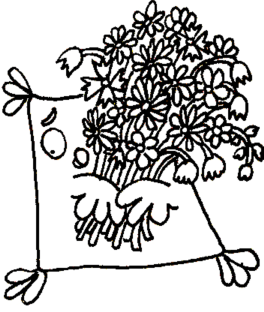
\includegraphics[scale=0.5]{15}}
\end{figure}
\end{SBSection*}

\end{song}

%\twocolumn
\begin{song}{Белая гвардия}{}{Белая гвардия}{Белая гвардия}{}{}

Проигрыш: (2 раза)\par 
\Ch{Am}{} \Ch{D}{} \Ch{G}{} \Ch{C}{} \Ch{Am}{} \Ch{H7}{} \Ch{Em}\\

\Ch{Em}{Белая} гвардия, белый снег,\par
\Ch{Am7}{Белая} музыка революций.\par
\Ch{D7}{Белая} женщина, нервный смех,\par
\Ch{G}{Белого} платья слегка коснуться.\par
 
Белой рукой распахнуть окно,\par
Белого света в нем не видя.\par
Белое выпить до дна вино,\par
В красную улицу в белом выйти.\\

Припев:\par
\ttКог\Ch{Em}{да} ты вернешься,\par
\ttВсе будет и\Ch{Am}{на}че, и нам бы узнать друг друга,\par
\ttКог\Ch{D7}{да} ты вернешься,\par
\ttА я не же\Ch{G}{на} и даже \Ch{H7}{не} подруга.\par
\ttКог\Ch{C}{да} ты вернешься,\par
\ttКо мне, так без\Ch{Am}{ум}но тебя любившей в прошлом,\par
\tt\Ch{D7}{Ко}гда ты вернешься -\par
\ttУвидишь, что ж\Ch{G}{ре}бий давно и не \Ch{E7}{нами} брошен.\\

Проигрыш.\\
 
\newpage
Сизые сумерки прошлых лет\par
Робко крадутся по переулкам.\par
В этом окне еле брезжит свет,\par
Ноты истрепаны, звуки гулки.\par
Тонкие пальцы срывают аккорд...\par
Нам не простят безрассудного дара.\par
Бьются в решетку стальных ворот\par
Пять океанов земного шара.\\

Припев. \par
Проигрыш.\\
 
Красный трамвай простучал в ночи,\par
Красный закат догорел в бокале,\par
Красные-красные кумачи\par
С красных деревьев на землю упали.\par
Я не ждала тебя в октябре,\par
Виделись сны, я листала сонник:\par
Красные лошади на заре\par
Били копытами о подоконник.\\

Припев:\par
\ttКогда ты вернешься,\par
\ttВсе будет иначе, и нам бы узнать друг друга,\par
\ttКогда ты вернешься,\par
\ttА я не жена и даже не подруга.\par
\ttКогда ты вернешься,\par
\ttВернешься в наш город обетованный,\par
\ttКогда ты вернешься -\par
\ttТакой невозможный и такой желанный?\\

Проигрыш.\par

\end{song}

%\twocolumn
\begin{song}{Перевал}{}{Песни у костра}{Песни у костра}{}{}


\Ch{Am}{Про}сто нечего нам \Ch{Dm}{боль}ше терять\par
\Ch{E}{Всё} нам вспомнится на \Ch{Am}{Страшном} суде.\par
Эта ночь легла, как \Ch{Dm}{тот} перевал,\par
\Ch{G}{За} которым испол\Ch{C}{нень}е надежд.\par
\Ch{A7}{Про}сто прожитое—про\Ch{Dm}{жи}то зря, \Ch{G}{}\par
Но не в этом, пони\Ch{C}{мае}шь ли, соль… \Ch{Am}{}\par
Слышишь, падают дож\Ch{Dm}{ди} октября.\par
\Ch{E}{Ви}дишь, старый дом сто\Ch{Am}{ит} средь лесов.\\

Мы затопим в доме печь, в доме печь,\par
Мы гитару позовем со стены.\par
Просто нечего нам больше беречь,\par
Ведь за нами все мосты сожжены.\par
Все мосты, все перекрёстки дорог,\par
Все прошёптанные тайны в ночи.\par
Каждый сделал все, что смог, все, что смог,\par
Мы об этом помолчим, помолчим.\\


И луна взойдет заплывшей свечой,\par
Ставни скрипнут  на ветру, на ветру.\par
Ах, как я тебя люблю горячо,\par
Это годы не сотрут, не сотрут.\par
Мы оставшихся друзей соберем,\par
Мы набьем картошкой старый рюкзак,\par
Люди спросят: "Что за шум, что за гам?"\par
Мы ответим: "Просто так,  просто так”...\\

\newpage

    Просто так идут дожди в октябре,\par
    И потеряны от счастья ключи.\par
    Это всё, конечно, мне, конечно, мне,\par
    Но об этом помолчим, помолчим.\par
    Просто прожитое—прожито зря,\par
    Но не в этом, понимаешь ли, соль…\par
    Слышишь, падают дожди октября.\par
    Видишь, старый дом стоит средь лесов.\par


\begin{SBSection*}
\begin{figure}[b!]
\center{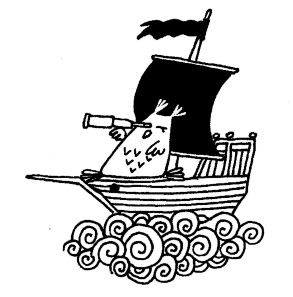
\includegraphics[scale=0.5]{22}}
\end{figure}
\end{SBSection*}

\end{song}

%\twocolumn
\begin{song}{Ленинградская (Все расстояния)}{}{Песни у костра}{Песни у костра}{}{}

\Ch{Am}{Все} расстоянья когда-нибудь в круг замы\Ch{E}{ка}ются,\par
\Ch{E}{Все} из разлук обязательно \Ch{E7}{встре}чей кон\Ch{Am}{ча}ются;\par
Должны про\Ch{Dm}{плыть} вокруг Зем\Ch{G}{ли,}\par
Вернуться в \Ch{C}{га}вань кораб\Ch{F}{ли,}\par   
Все поез\Ch{Dm}{да} в свои вер\Ch{E}{нуть}ся горо\Ch{Am}{да.}\\
 
Шумный вокзал то встречает друзей , то прощается,\par
Мы расстаемся, но снова назад возвращаемся -\par
Чтоб снова встать в огромный круг,\par
И снова знать, что рядом друг ,\par
И песни петь, чтоб больше не было разлук.\\
 
Все расстоянья когда-нибудь в круг замыкаются,\par
Все из разлук обязательно встречей кончаются;\par
И через год, и через пять,\par
Мы с вами встретимся опять,\par
Ничто не сможет нашей дружбе помешать.\par

\end{song}

%\twocolumn
\begin{song}{Десять капель}{}{Танцы Минус}{Танцы Минус}{}{}

Проигрыш: (2 раза)\par 
\Ch{C}{} \Ch{E}{} \Ch{Am}{} \Ch{F}{} \Ch{C}{} \Ch{E}{} \Ch{Am}{} \Ch{F}{}

\Ch{C}{Де}сять капель дож\Ch{E}{дя} у тебя на пле\Ch{Am}{че}\par
Ты забыла свой \Ch{F}{зонт,} ты спешила ко \Ch{C}{мне.}\par
Десять капель дож\Ch{E}{дя} на плече у те\Ch{Am}{бя,}\par
Десять капель люб\Ch{F}{ви,} десять капель ог\Ch{C}{ня}\\

Припев:\\(Три первых слова в припеве дублируются вторым голосом)\par
\tt\Ch{C}{Т}воя\Ch{E}{} ладо\Ch{Am}{нь} горит\Ch{F}{} в моих руках\par
\tt\Ch{C}{Л}юбви\Ch{E}{ }пож\Ch{Am}{ар} горит в тво\Ch{F}{их} глазах\\

Проигрыш.\\

Время делает шаг, время делает круг\par
Мы забудем друзей, мы забудем подруг\par
Просто выпьем вина из любви и огня\par
Десять капель меня, десять капель тебя\\

Припев.\\

Голос твой в тишине околдует меня\par
Ярким жарким огнем стану я до утра\par
Ты прикажешь гори, и я вспыхну любя\par
В этом пламени ты, в этом пламени я.\par

\end{song}

%\twocolumn
\begin{song}{Макет}{}{Песни у костра}{Сказка}{}{}
sadfsfthanks,\par
\begin{SBOpGroup}
asdas\
\end{SBOpGroup}
\begin{SBSection*}fdf\end{SBSection*}
\begin{SBVerse*}\end{SBVerse*}
\begin{SBChorus*}\end{SBChorus*}

\begin{SBOccurs}{23}
dsf
\end{SBOccurs}

\begin{SBSection*}
\begin{figure}[b!]
\center{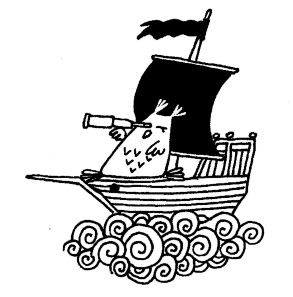
\includegraphics[scale=0.5]{22}}
\end{figure}
\end{SBSection*}
\end{song}

\mainmatter

\renewcommand{\footrulewidth}{0.0pt}
\renewcommand{\item}{\par\hangindent=40pt}
\renewcommand{\subitem}{\par\hangindent=40pt \hspace*{20pt}}
\renewcommand{\subsubitem}{\par\hangindent=40pt \hspace*{30pt}}

\newpage
\raggedright%\documentclass[a5paper,11pt]{book}
%\usepackage{fancyhdr}
%\usepackage[chordbk]{songbook}
%
%\usepackage[T2A]{fontenc}
%\usepackage[utf8]{inputenc}
%\usepackage[russian]{babel}
%
%\title{A Church Songbook}
%\author{}
%\date{Revised:  \RevDate}
%
%\newcommand{\RelDate}{13 November'19}
%\newcommand{\RevDate}{\today}

\documentclass[11pt,a5paper]{book}
\usepackage[a5paper]{geometry}
\usepackage[chordbk]{songbook}
\usepackage[T2A]{fontenc}
\usepackage[utf8]{inputenc}
\usepackage[russian]{babel}
\usepackage{cmap} % для работы поиска кириллицы в pdf

%\usepackage{amsmath,amsthm,amssymb}
%\usepackage{mathtext}


\usepackage[pdftex]{graphicx}
\usepackage{lscape}
%\usepackage{vmargin}
\usepackage{textcomp}
\usepackage{setspace}
%\usepackage{marvosym}
\usepackage{gensymb} %%%for \micro tag
\usepackage{upgreek} %%% \upmu
\usepackage{tipa}
\usepackage{phonetic}
%\usepackage[greek,english]{babel}
\usepackage{threeparttable}
\usepackage{multirow}
\usepackage{harvard}
\usepackage{longtable}
\renewcommand{\sectionmark}[1]{\markright{#1}}
\renewcommand{\chaptermark}[1]{\markboth{#1}{}}
\addto\captionsenglish{\renewcommand{\bibname}{References}}
\usepackage{latexsym,fancyhdr}

\newcommand{\RelDate}{26 Апреля'1984}
\newcommand{\RevDate}{\today}

%%%
% C.C.L.I. license number definition; for copyright licensing info.
% One of these macros will be manually inserted into the {CpyRt}
% parameter of the {song} environment.
%
%       \CCLInumber - The actual copyright license number.  Don't
%               insert this command in the {CpyRt} parameter, use one
%               of the others.
%       \CCLIed - Indicates a song falls under our CCLI license.
%       \NotCCLIed - Indicates a song doesn't fall under our CCLI
%               license.  Public Domain songs fall into this category.
%       \PGranted - We have received specific permission from the
%               copyright holder to use this song.
%       \PPending - We are in the process of obtaining permission to
%               use this song.
%%%
\newcommand{\CCLInumber}{Your CCLI Number}
\newcommand{\CCLIed}{{\CpyRtInfoFont (CCLI \CCLInumber)}}
\newcommand{\NotCCLIed}{\relax}
\newcommand{\PGranted}{\relax}
\newcommand{\PPending}{{\CpyRtInfoFont (Permission Pending)}}

%%%
% Title page information.
%%%
\title{ Сказочный песенник}
\author{}
\date{Созданно:  \RevDate}


%%%
% Define fonts to use in the headers and footers of the songbook.
%%%
\newcommand{\LHeadFont}{\normalsize}            % = cmr12  at 12pt
\newcommand{\CHeadFont}{\normalsize\rm}         % = cmr12  at 12pt
\newcommand{\RHeadFont}{\normalsize}            % = cmr12  at 12pt
\newcommand{\LFootFont}{\scriptsize}            % = cmr8   at  8pt
\newcommand{\CFootFont}{\tiny\myTinySF}         % = cmss8  at  8pt
\newcommand{\RFootFont}{\scriptsize}            % = cmr8   at  8pt

%%%
% Turn on and define fancy page heading/footing definition.
%%%
\pagestyle{fancy}

\ifChordBk
  % It's a words & chords songbook...
%  \addtolength{\headwidth}{\marginparsep}
%  \addtolength{\headwidth}{\marginparwidth}
  \renewcommand{\headrulewidth}{0.0pt}
  \renewcommand{\footrulewidth}{0.0pt}
%  \fancyhead[LE,RO]{\LHeadFont\emph{\leftmark\/}}
%  \fancyhead[CE,CO]{\CHeadFont\thepage}
  \fancyhead[RE,LO]{~}
\else\ifOverhead
  % It's an overhead...
  \renewcommand{\footrulewidth}{0pt}
  \renewcommand{\headrulewidth}{0pt}
  \fancyhead[LE,RO]{}
  \fancyhead[CE,CO]{}
  \fancyhead[RE,LO]{}
\else\ifWordBk
  % It's a words only songbook...
  \addtolength{\headwidth}{\marginparsep}
  \addtolength{\headwidth}{\marginparwidth}
  \renewcommand{\headrulewidth}{0.0pt}
  \renewcommand{\footrulewidth}{0.0pt}
  \fancyhead[LE,RO]{\LHeadFont A Church Songbook}
  \fancyhead[CE,CO]{\CHeadFont\thepage}
  \fancyhead[RE,LO]{\RHeadFont\RelDate}
\fi\fi\fi

%\fancyfoot[LE,RO]{\LFootFont Property of The Church}
%\ifSongEject
%  \fancyfoot[CE,CO]{\CFootFont \RevDate}
%\else
%  \fancyfoot[CE,CO]{\CFootFont}
%\fi
%\fancyfoot[RE,LO]{\RFootFont Material used by permission.}

%%%
% Turn on/off index-file generation.  Uncomment the \makeindex line to
% turn index generation on;  comment it out to turn index generation
% off.
%%%
\makeTitleIndex         %% Title and First Line Index.
\makeTitleContents      %% Table of Contents.
\makeKeyIndex           %% Index of song by key.
\graphicspath{{img/}} % папка с картинками
\DeclareGraphicsExtensions{.pdf,.png,.jpg} % форматы, которые будем считать картинками

%\newenvironment{song}[7][Y]{
%% Comment markers to negate
%\if#1Y\ExcludeSongfalse\else\ExcludeSongtrue\fi% the newline.
%\ifPrintAllSongs\ExcludeSongfalse\fi
%\SongMarkboth{\relax}{\relax}
%\SBinSongEnvtrue
%\renewcommand{\SBinSongEnv}{\True}
%\ifWordsOnly
%	\setlength{\parindent}{0pt}
%\fi

%%%
% Redefine fonts from SongBook style that I don't like.
%%%
\font\myTinySF=cmss8 at 8pt
\renewcommand{\CpyRtInfoFont}{\tiny\myTinySF}


%
%\font\myTinySF=cmss8    at  8pt
%\font\myHugeSF=cmssbx10 at 25pt
%\renewcommand{\CpyRtInfoFont}{\tiny\myTinySF}
%\newcommand{\myTitleFont}{\Huge\myHugeSF}
%\newcommand{\mySubTitleFont}{\large\sf}

%%% Работа с русским языком
%\usepackage[no-math]{fontspec}      %% подготавливает загрузку шрифтов Open Type, True Type и др.
%\defaultfontfeatures{Ligatures={TeX},Renderer=Basic}  %% свойства шрифтов по умолчанию
%\setmainfont[Ligatures={TeX,Historic}]{Times New Roman} %% задаёт основной шрифт документа
%\setsansfont{Helvetica Neue}                    %% задаёт шрифт без засечек

%\newfontfamily{\allods}{AllodsWest}

\newcommand{\SBPubDomm}{~}
\renewcommand{\CpyRt}[3][Y]{%
\if#1Y\begin{center}\fi
\if\blank{#2}%
\if\blank{#3}%
{\CpyRtFont\copyright \SBUnknownTag{} \CpyRtInfoFont}%
\else
{\CpyRtFont\copyright \SBUnknownTag{} \CpyRtInfoFont #3}%
\fi%
\else%
\ifthenelse{\equal{#2}{\SBPubDomm}}
{%then
{\CpyRtFont #2 \CpyRtInfoFont #3}%
}{%else
{\CpyRtFont #2 \CpyRtInfoFont #3}%
}%fi
\fi%
\if#1Y\end{center}\fi
}


\newcommand{\SBUnknownTagg}{~}
\renewcommand{\WAndM}[2][Y]{~}
\renewcommand{\WAndM}[2][Y]{%
\if#1Y\begin{center}\fi
\if\blank{#2}%
{\SBUnknownTagg}%
\else
{~}%
\fi
\if#1Y\end{center}\fi
}

\renewcommand{\STitle}[3][Y]{%
\setcounter{SBVerseCnt}{0}%
\setcounter{SBSectionCnt}{0}%
\ifExcludeSong\relax%
	\else\keyIndex{{\protect\sbChord#3\protect\relax} -- #2}{\theSBSongCnt}\fi%
	\vspace{\SpaceAboveSTitle}%
\if#1Y\begin{center}\fi
	{}{\STitleFont\LARGE #2}%
	\ifWordsOnly\relax\else\fi%
	\if#1Y\end{center}\fi
\STitleMarkboth{#2}{\relax}%
}


%\renewenvironment{SBOpGroup}{%
%	\sbSetsbBaselineSkipAmt%
%	\bgroup%
%	\begin{list}{\hbox{}}
%	  {\setlength {\leftmargin}
%		{\HangAmt}
%		\setlength{\itemindent}
%			{-\HangAmt}
%		\setlength{\listparindent}{-\HangAmt}
%		\setlength{\topsep}{0pt}
%		\setlength{\parsep}{0pt}
%		\setlength{\labelwidth}{0pt}
%		\setlength{\labelsep}{0pt}
%		\setlength{\baselineskip} {\sbBaselineSkipAmt}
%	}%\item}
%{\end{list}%
\newcommand{\SBChorusTagg}{Припев}
\renewenvironment{SBChorus}{%
\sbSetsbBaselineSkipAmt%
\bgroup%
\SBChorusMarkright{\SBChorusTag}
\begin{list}{{\SBChorusTagFont\SBChorusTagg}}
{\setlength {\leftmargin}
{\LeftMarginSBChorus + \HangAmt}
\setlength{\itemindent}
{-\HangAmt}
\setlength{\listparindent}{-\HangAmt}
\setlength{\parsep}
{0pt}
\setlength{\baselineskip} {\sbBaselineSkipAmt}
}%
\item}
{\end{list}%
\egroup%
\SpaceAfterChorus%
}

\renewcommand{\tt}{\indent \indent}
%\renewcommand{\nt}{\noindent}


\usepackage{amsmath}

\makeArtistIndex
\makeTitleIndex         %% Title and First Line Index.
\makeTitleContents      %% Table of Contents.
\makeKeyIndex           %% Index of song by key.
%\usepackage{printallsongs}

\begin{document} 
\maketitle

\mainmatter


\begin{song}{Вожатский гимн}{}{Сказка}{Сказка}{}{}

По \Ch{Am}{ла}герю подъём, нас горн зовёт!\par
Забудь о том, что ночь была бес\Ch{C}{сон}ною\par
Смо\Ch{Dm}{чи} водою \Ch{G}{ве}ки воспа\Ch{C}{лён}\Ch{F}{ные}\par    
По\Ch{Dm}{вя}зывай свой \Ch{E}{галс}тук — и впе\Ch{Am (A7)}{рёд!}\par
Смо\Ch{Dm}{чи} водою \Ch{G}{ве}ки воспа\Ch{C}{лён}\Ch{F}{ные}\par    
По\Ch{Dm}{вя}зывай свой \Ch{E}{галс}тук — и впе\Ch{Am (A7)}{рёд!}\par

%	\begin{SBChorus*}
\ttНе\Ch{E}{про}сто воспитывать \Ch{Am}{но}вых людей,\par
\ttНу \Ch{E}{что} ж, это наша с то\Ch{Am}{бою} свя\Ch{A7}{ты}ня.\par
\ttМой \Ch{Dm}{друг}, нам до\Ch{G}{ве}рили \Ch{C}{ду}ши де\Ch{F}{тей},\par
\ttИх \Ch{Dm}{ра}достный \Ch{Am}{смех} нам на\Ch{E}{гра}да от\Ch{Am}{ны}не.\par
\ttМой \Ch{Dm}{друг}, нам до\Ch{G}{ве}рили \Ch{C}{ду}ши де\Ch{F}{тей},\par
\ttИх \Ch{Dm}{ра}достный \Ch{Am}{смех} нам на\Ch{E}{гра}да от\Ch{Am}{ны}не.\\
%\end{SBChorus*}

Отбой, засыпает детвора.\par
Взгляни на их улыбки полусонные,\par
Пускай им снятся острова зелёные,\par
А нам опять работать до утра!\par
Пускай им снятся острова зелёные,\par
А нам опять работать до утра!\par

\tt И пусть от бессилья затихнешь не раз,\par
\ttИ голос усталый до хрипа натружен,\par
\ttПусть будут умней и счастливее нас\par
\ttТе дети, в которых вложили мы души!\par
\ttПусть будут умней и счастливее нас\par
\ttТе дети, в которых вложили мы души!

\end{song}

\begin{song}{Сказка в неглиже}{}{Сказка}{Сказка}{}{}

Есть у \Ch{C}{каж}дого добрая сказка в ду\Ch{F}{ше,}\par 
Надо \Ch{G}{толь}ко прочесть этой сказки стра\Ch{C}{ни}цы.\par
В тиши\Ch{C}{не}, разо\Ch{C7}{де}тая вся в негли\Ch{F}{же,}\par
Пусть на\Ch{G}{ве}ки она, пусть на\Ch{F}{ве}ки она сохра\Ch{C}{ни}тся. \Ch{C7}{ }\par 
В тиши\Ch{F}{не,} разо\Ch{G}{де}тая вся в негли\Ch{C}{же,} \Ch{Am}{}\par
Пусть на\Ch{F}{ве}ки она, пусть на\Ch{G}{ве}ки она сохра\Ch{C}{ни}тся.\\


\ttЭту сказку пред другом раскрыть поспеши,\par
\ttА врагу не спеши эту сказку поведать.\par
\ttПусть растут и читают ее малыши.\par
\ttБудь добрей, и тебя минут всякие беды.\par
\ttПусть растут и читают ее малыши.\par
\ttБудь добрей, и тебя минут всякие беды.\\


\Ch{C7}{}Будет \Ch{F}{мно}го распутий, \Ch{G}{до}рог и тре\Ch{C}{вог.}\Ch{Am}{}\par
На вис\Ch{F}{ки} твои ляжет \Ch{G}{не}тающий \Ch{C}{ин}ей, \Ch{C7}{}\par
И пой\Ch{F}{мёшь,} научившись чи\Ch{G}{тать} между \Ch{C}{строк:} \Ch{Am}{}\par
Даже \Ch{F}{гнус}ный злодей \Ch{G}{в} этой сказке не\Ch{C}{ви}нен. \Ch{C7}{}\par
И пой\Ch{F}{мёшь,} научившись чи\Ch{G}{тать} между ст\Ch{C}{рок:} \Ch{A}{}\par
Даже \Ch{F}{гнус}ный злодей \Ch{G}{в} этой сказке не\Ch{C}{ви}нен.\\

\Ch{C}{} \Ch{G}{} \Ch{F}{} \Ch{G}{} \Ch{C}{} \Ch{C7}{}\par
\Ch{C}{} \Ch{G}{} \Ch{F}{} \Ch{G}{} \Ch{C}{}
\end{song}

%\twocolumn
\begin{song}{Вожатский марш}{}{Сказка}{Сказка}{}{}

Есть на\Ch{Am}{род} у нас весёлый,\par
Самой \Ch{C}{луч}шей в мире пробы,\par
Песни \Ch{G}{петь} всегда мас\Ch{C}{так.}\Ch{A7}{}\par
Он всег\Ch{Dm}{да} всего добьётся,\par
Он Вожа\Ch{Am}{ты}ми зовётся,\par
\Ch{E}{Так} и только \Ch{Am (A7)}{так!}\par
Он всег\Ch{Dm}{да} всего добьётся,\par
Он Во\Ch{Am}{жа}тыми зовётся,\par
\Ch{E}{Так} и только \Ch{Am (A7)}{так!}\\

Домосед привязан к дому\par
И по случаю такому,\par
Он из дома — ни на шаг!\par
А вожатый — он в дороге,\par
Он готов в огонь и в воду,\par
Так и только так!\par
А вожатый — он в дороге,\par
Он готов в огонь и в воду,\par
Так и только так!\\
\newpage
Жадный денежки считает,\par
Все считает и считает,\par
К пятаку кладет пятак.\par
А вожатый деньги тратит,\par
Не боясь, что их не хватит,\par
Так и только так!\par
А вожатый деньги тратит,\par
Не боясь, что их не хватит,\par
Так и только так!\\

Холостяк в любовь не верит,\par
Все не верит и не верит,\par
Потому что холостяк.\par
А вожатых не влюблённых\par
Не найдёшь определённо,\par
Так и только так!\par
А вожатых не влюблённых\par
Не найдёшь определённо,\par
Так и только так!\par

\begin{SBSection*}
\begin{figure}[b!]
\center{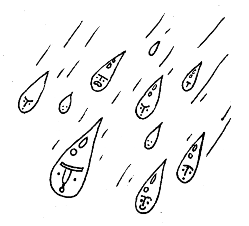
\includegraphics[scale=0.5]{16}}
\end{figure}
\end{SBSection*}
\end{song}

%\twocolumn
\begin{song}{Двадцать дней}{}{Сказка}{Сказка}{}{}


Двадцать дн\Ch{Dm}{ей} – это смена без дня.\par
“Маловато”,– вам скажут друзь\Ch{Gm}{я,}\par
А вожатый отв\Ch{C}{ет}ит люб\Ch{F}{ой}:\par
Это ср\Ch{Gm}{ок} очень д\Ch{A}{аж}е больш\Ch{Dm}{ой!}\\
 

Припев:\par
\ttМожно з\Ch{Gm C}{а-а-а-а} него усп\Ch{Dm}{ет}ь,\par
\ttНаприм\Ch{Gm}{ер,} полмилли\Ch{A}{он}а песен сп\Ch{Dm}{еть,}\par
\ttНо не к\Ch{Gm}{ажд}ый ведь поймет,\par
\ttКак так быстро раскрыв\Ch{A}{ат}ься может р\Ch{Dm}{от!}\\


Для полярника это не срок:\par
Не успеет просохнуть носок.\par
А вожатый успеет подряд \par
Вымыть, высушить сотню ребят!\\

Припев:\par
\ttВедь за смену, как за год \par
\ttСтолько разных мелочей произойдет,\par
\ttНо пока что нам везет,\par
\ttНас начальство для чего-то бережёт.\\


\newpage
Хоть и длинными кажутся дни,\par
Но как миг пролетели они.\par
Будешь долго потом вспоминать,\par
Как в отбой ты любил слово «СПАААТЬ!!!»\\

Припев:\par
\tt          	— Говорят за двадцать дней \par
\tt          	Все узнаешь о напарнице своей…\par
\tt          	— Только это ерунда,\par
\tt          	Обо всем ты не узнаешь никогда!\\

Смена вряд ли даст ответ:\par
Ты нашел свое призванье или нет.\par
Так что надо продолжать,\par
Двадцать раз по двадцать суток отсчитать!\\

\begin{SBSection*}
\begin{figure}[b!]
\center{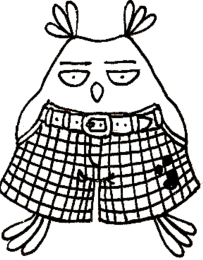
\includegraphics[scale=0.5]{17}}
\end{figure}
\end{SBSection*}

\end{song}

%\twocolumn
\begin{song}{Непогода}{}{Павел Смеян}{Павел Смеян}{}{}

\Ch{D}{Из}менения в природе \Ch{G}{пр}оисходят г\Ch{A}{од} от года,\par
\Ch{D}{Не}погода нынче в моде,\Ch{G}{} н\Ch{F#7}{епог}ода, непогода,\par
\Ch{}Hm{Слов}но из вод\Ch{F#7}{опро}вода \Ch{D7}{ль}ёт на нас с неб\Ch{G}{ес} во\Ch{Hm}{да…}\par
Полг\Ch{G}{од}а плох\Ch{A}{ая} пог\Ch{D}{од}а, \Ch{Hm}{пол}го\Ch{G}{да} — совс\Ch{A}{ем} нику\Ch{D}{да}.\par
Полг\Ch{G}{од}а плох\Ch{A}{ая} пог\Ch{D}{од}а, \Ch{Hm}{пол}го\Ch{G}{да} — сов\Ch{F#7}{сем} нику\Ch{Hm}{да.}\\


\SBChorusTagg:\par
\ttНикуда, нику\Ch{Em}{да н}ельз\Ch{A}{я} укр\Ch{D}{ы}ться н\Ch{Hm}{ам,}\par
\ttНо откладывать ж\Ch{Em}{изнь} ни\Ch{A}{как} нель\Ch{D}{зя}, \Ch{Hm}{}\par
\ttНикуда, нику\Ch{Em}{да, н}о зн\Ch{A}{ай}, что гд\Ch{D}{е}-то т\Ch{Hm}{ам}\par
\ttКто-то ищет теб\Ch{G}{я} сре\Ch{F#7}{ди д}ожд\Ch{Hm}{я.} \Ch{A}{}\\


Грома грозные раскаты от заката до восхода,\par
За грехи людские плата — непогода, непогода,\par
Не ангина, не простуда, посерьёзнее беда.\par
Полгода плохая погода, полгода — совсем никуда\par,
Полгода плохая погода, полгода — совсем никуда.\\\


\SBChorusTagg:\par
\ttНикуда, нику\Ch{Em}{да н}ельз\Ch{A}{я} укр\Ch{D}{ы}ться н\Ch{Hm}{ам,}\par
\ttНо откладывать ж\Ch{Em}{изнь} ни\Ch{A}{как} нель\Ch{D}{зя}, \Ch{Hm}{}\par
\ttНикуда, нику\Ch{Em}{да, н}о зн\Ch{A}{ай}, что гд\Ch{D}{е}-то т\Ch{Hm}{ам}\par
\ttКто-то ищет теб\Ch{G}{я} сре\Ch{F#7}{ди д}ожд\Ch{Hm}{я.} \Ch{A}{}\\


\end{song}

%\twocolumn
\begin{song}{Птенцы}{}{Сказка}{Сказка}{}{}

\Ch{Am}{}  \Ch{Am}{}

Как птенцы из гнез\Ch{Dm}{да} мы \Ch{E}{вы}па\Ch{Am}{ли.}\par
Ты не бойся при\Ch{Dm}{хо}да \Ch{G}{ве}че\Ch{C}{ра.}\par
Под та\Ch{A7}{ки}ми боль\Ch{F}{ши}ми \Ch{A7}{ли}па\Ch{Dm}{ми}\par
Нам с то\Ch{F}{бой} опа\Ch{Dm}{сать}ся \Ch{F}{не}\Ch{E}{че}\Ch{Am}{го.}\\
 
Под такими густыми звёздами -\par
Разве их не для нас рассыпали,\par
Мы не против гнездовья - просто мы\par
Из него ненароком выпали.\\

Это только вначале кажется,\par
Что без дома прожить нельзя никак,\par
Что важней пропитанья кашица,\par
Чем огромные звёзды на небе.\\

Ты не бойся ни тьмы, ни холода.\par
Будет день и найдётся пища нам,\par
Мы ещё пролетим над городом\par
На крыле до небес возвышенном.\\

Пролетим ещё - эка невидаль\par
Над Нью-Йорком, Парижем, Триполи\par
И над липой, откуда некогда,\par
Как птенцы из гнезда мы выпали.\\

Как птенцы из гнезда мы выпали.\par
Ты не бойся прихода вечера.\par
Под такими большими липами\par
Нам с тобой опасаться нечего.\\

\end{song}

%\twocolumn
\begin{song}{Продавец зонтиков}{}{Веня Дркин}{Веня Дркин}{}{}

\Ch{Am}{Город} этот выдумал о\Ch{Dm}{дин} художник,\par
\Ch{G}{Лю}ди в нем не знали, что та\Ch{C}{ко}е дождик.\par
\Ch{A7}{Про}сто не слыхали, что та\Ch{Dm}{ко}е зонтик –\par
\Ch{E7}{Вот} такие люди жили в \Ch{Am}{го}роде том.\par
И один чудак, в старый плащ одетый,\par
Продавал там зонтики зимой и летом,\par
Продавал там зонтики зимой и летом\par
И такую песенку он напевал:\\

\SBChorusTagg:\par
\tt“Господа, купите зонтик.\par
\ttБелый зонтик, красный зонтик,\par
\ttЖелтый зонтик, синий зонтик –\par
\ttМожет пригодится вам.”\\

Были домики у них из пластилина,\par
Из пустых коробочек автомашины,\par
И, не опасаясь никакой ангины,\par
Маленькие люди жили в городе том.\par
Маленькие были у людей заботы:\par
Шли они в кино или в театр с работы.\par
Вечером в подъезде целовался кто-то.\par
Все шутили и смеялись над стариком.\\


\SBChorusTagg.\\

\newpage

Маленькое небо как-то вдруг намокло,\par
В крошечных домишках задрожали стекла,\par
И огромный дождь пошел гулять по крышам,\par
Сразу все схватили насморк в городе том.\par
Вспомнили тут люди о торговце старом,\par
Кинулись искать его по всем базарам,\par
Но исчез торговец со своим товаром.\par
Только песенка осталась в память о нем:\\

\SBChorusTagg.\par

\begin{SBSection*}
\begin{figure}[b!]
\center{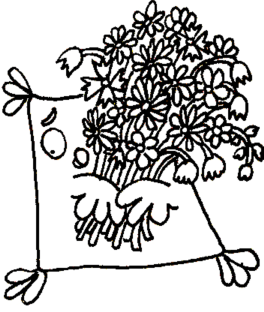
\includegraphics[scale=0.5]{15}}
\end{figure}
\end{SBSection*}

\end{song}

%\twocolumn
\begin{song}{Белая гвардия}{}{Белая гвардия}{Белая гвардия}{}{}

Проигрыш: (2 раза)\par 
\Ch{Am}{} \Ch{D}{} \Ch{G}{} \Ch{C}{} \Ch{Am}{} \Ch{H7}{} \Ch{Em}\\

\Ch{Em}{Белая} гвардия, белый снег,\par
\Ch{Am7}{Белая} музыка революций.\par
\Ch{D7}{Белая} женщина, нервный смех,\par
\Ch{G}{Белого} платья слегка коснуться.\par
 
Белой рукой распахнуть окно,\par
Белого света в нем не видя.\par
Белое выпить до дна вино,\par
В красную улицу в белом выйти.\\

Припев:\par
\ttКог\Ch{Em}{да} ты вернешься,\par
\ttВсе будет и\Ch{Am}{на}че, и нам бы узнать друг друга,\par
\ttКог\Ch{D7}{да} ты вернешься,\par
\ttА я не же\Ch{G}{на} и даже \Ch{H7}{не} подруга.\par
\ttКог\Ch{C}{да} ты вернешься,\par
\ttКо мне, так без\Ch{Am}{ум}но тебя любившей в прошлом,\par
\tt\Ch{D7}{Ко}гда ты вернешься -\par
\ttУвидишь, что ж\Ch{G}{ре}бий давно и не \Ch{E7}{нами} брошен.\\

Проигрыш.\\
 
\newpage
Сизые сумерки прошлых лет\par
Робко крадутся по переулкам.\par
В этом окне еле брезжит свет,\par
Ноты истрепаны, звуки гулки.\par
Тонкие пальцы срывают аккорд...\par
Нам не простят безрассудного дара.\par
Бьются в решетку стальных ворот\par
Пять океанов земного шара.\\

Припев. \par
Проигрыш.\\
 
Красный трамвай простучал в ночи,\par
Красный закат догорел в бокале,\par
Красные-красные кумачи\par
С красных деревьев на землю упали.\par
Я не ждала тебя в октябре,\par
Виделись сны, я листала сонник:\par
Красные лошади на заре\par
Били копытами о подоконник.\\

Припев:\par
\ttКогда ты вернешься,\par
\ttВсе будет иначе, и нам бы узнать друг друга,\par
\ttКогда ты вернешься,\par
\ttА я не жена и даже не подруга.\par
\ttКогда ты вернешься,\par
\ttВернешься в наш город обетованный,\par
\ttКогда ты вернешься -\par
\ttТакой невозможный и такой желанный?\\

Проигрыш.\par

\end{song}

%\twocolumn
\begin{song}{Перевал}{}{Песни у костра}{Песни у костра}{}{}


\Ch{Am}{Про}сто нечего нам \Ch{Dm}{боль}ше терять\par
\Ch{E}{Всё} нам вспомнится на \Ch{Am}{Страшном} суде.\par
Эта ночь легла, как \Ch{Dm}{тот} перевал,\par
\Ch{G}{За} которым испол\Ch{C}{нень}е надежд.\par
\Ch{A7}{Про}сто прожитое—про\Ch{Dm}{жи}то зря, \Ch{G}{}\par
Но не в этом, пони\Ch{C}{мае}шь ли, соль… \Ch{Am}{}\par
Слышишь, падают дож\Ch{Dm}{ди} октября.\par
\Ch{E}{Ви}дишь, старый дом сто\Ch{Am}{ит} средь лесов.\\

Мы затопим в доме печь, в доме печь,\par
Мы гитару позовем со стены.\par
Просто нечего нам больше беречь,\par
Ведь за нами все мосты сожжены.\par
Все мосты, все перекрёстки дорог,\par
Все прошёптанные тайны в ночи.\par
Каждый сделал все, что смог, все, что смог,\par
Мы об этом помолчим, помолчим.\\


И луна взойдет заплывшей свечой,\par
Ставни скрипнут  на ветру, на ветру.\par
Ах, как я тебя люблю горячо,\par
Это годы не сотрут, не сотрут.\par
Мы оставшихся друзей соберем,\par
Мы набьем картошкой старый рюкзак,\par
Люди спросят: "Что за шум, что за гам?"\par
Мы ответим: "Просто так,  просто так”...\\

\newpage

    Просто так идут дожди в октябре,\par
    И потеряны от счастья ключи.\par
    Это всё, конечно, мне, конечно, мне,\par
    Но об этом помолчим, помолчим.\par
    Просто прожитое—прожито зря,\par
    Но не в этом, понимаешь ли, соль…\par
    Слышишь, падают дожди октября.\par
    Видишь, старый дом стоит средь лесов.\par


\begin{SBSection*}
\begin{figure}[b!]
\center{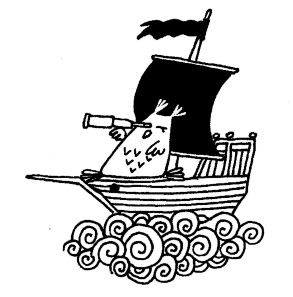
\includegraphics[scale=0.5]{22}}
\end{figure}
\end{SBSection*}

\end{song}

%\twocolumn
\begin{song}{Ленинградская (Все расстояния)}{}{Песни у костра}{Песни у костра}{}{}

\Ch{Am}{Все} расстоянья когда-нибудь в круг замы\Ch{E}{ка}ются,\par
\Ch{E}{Все} из разлук обязательно \Ch{E7}{встре}чей кон\Ch{Am}{ча}ются;\par
Должны про\Ch{Dm}{плыть} вокруг Зем\Ch{G}{ли,}\par
Вернуться в \Ch{C}{га}вань кораб\Ch{F}{ли,}\par   
Все поез\Ch{Dm}{да} в свои вер\Ch{E}{нуть}ся горо\Ch{Am}{да.}\\
 
Шумный вокзал то встречает друзей , то прощается,\par
Мы расстаемся, но снова назад возвращаемся -\par
Чтоб снова встать в огромный круг,\par
И снова знать, что рядом друг ,\par
И песни петь, чтоб больше не было разлук.\\
 
Все расстоянья когда-нибудь в круг замыкаются,\par
Все из разлук обязательно встречей кончаются;\par
И через год, и через пять,\par
Мы с вами встретимся опять,\par
Ничто не сможет нашей дружбе помешать.\par

\end{song}

%\twocolumn
\begin{song}{Десять капель}{}{Танцы Минус}{Танцы Минус}{}{}

Проигрыш: (2 раза)\par 
\Ch{C}{} \Ch{E}{} \Ch{Am}{} \Ch{F}{} \Ch{C}{} \Ch{E}{} \Ch{Am}{} \Ch{F}{}

\Ch{C}{Де}сять капель дож\Ch{E}{дя} у тебя на пле\Ch{Am}{че}\par
Ты забыла свой \Ch{F}{зонт,} ты спешила ко \Ch{C}{мне.}\par
Десять капель дож\Ch{E}{дя} на плече у те\Ch{Am}{бя,}\par
Десять капель люб\Ch{F}{ви,} десять капель ог\Ch{C}{ня}\\

Припев:\\(Три первых слова в припеве дублируются вторым голосом)\par
\tt\Ch{C}{Т}воя\Ch{E}{} ладо\Ch{Am}{нь} горит\Ch{F}{} в моих руках\par
\tt\Ch{C}{Л}юбви\Ch{E}{ }пож\Ch{Am}{ар} горит в тво\Ch{F}{их} глазах\\

Проигрыш.\\

Время делает шаг, время делает круг\par
Мы забудем друзей, мы забудем подруг\par
Просто выпьем вина из любви и огня\par
Десять капель меня, десять капель тебя\\

Припев.\\

Голос твой в тишине околдует меня\par
Ярким жарким огнем стану я до утра\par
Ты прикажешь гори, и я вспыхну любя\par
В этом пламени ты, в этом пламени я.\par

\end{song}

%\twocolumn
\begin{song}{Макет}{}{Песни у костра}{Сказка}{}{}
sadfsfthanks,\par
\begin{SBOpGroup}
asdas\
\end{SBOpGroup}
\begin{SBSection*}fdf\end{SBSection*}
\begin{SBVerse*}\end{SBVerse*}
\begin{SBChorus*}\end{SBChorus*}

\begin{SBOccurs}{23}
dsf
\end{SBOccurs}

\begin{SBSection*}
\begin{figure}[b!]
\center{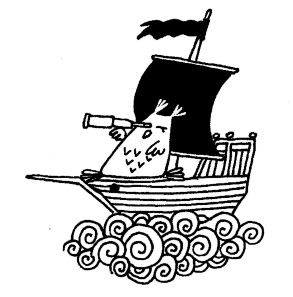
\includegraphics[scale=0.5]{22}}
\end{figure}
\end{SBSection*}
\end{song}

\mainmatter

\renewcommand{\footrulewidth}{0.0pt}
\renewcommand{\item}{\par\hangindent=40pt}
\renewcommand{\subitem}{\par\hangindent=40pt \hspace*{20pt}}
\renewcommand{\subsubitem}{\par\hangindent=40pt \hspace*{30pt}}

\newpage
\raggedright\input{/home/p_a/git/ska3ka/ps.adx}

\centering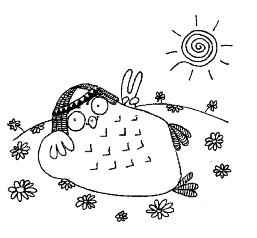
\includegraphics[scale=0.5]{10}

\newpage
\raggedright\input{/home/p_a/git/ska3ka/ps.tdx}

\centering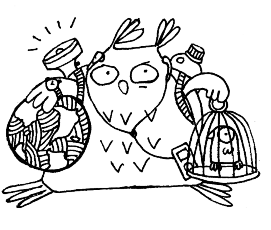
\includegraphics[scale=0.5]{11}

\end{document}


\centering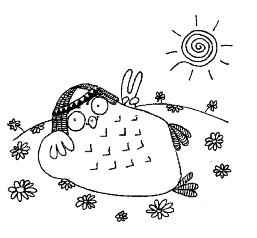
\includegraphics[scale=0.5]{10}

\newpage
\raggedright%\documentclass[a5paper,11pt]{book}
%\usepackage{fancyhdr}
%\usepackage[chordbk]{songbook}
%
%\usepackage[T2A]{fontenc}
%\usepackage[utf8]{inputenc}
%\usepackage[russian]{babel}
%
%\title{A Church Songbook}
%\author{}
%\date{Revised:  \RevDate}
%
%\newcommand{\RelDate}{13 November'19}
%\newcommand{\RevDate}{\today}

\documentclass[11pt,a5paper]{book}
\usepackage[a5paper]{geometry}
\usepackage[chordbk]{songbook}
\usepackage[T2A]{fontenc}
\usepackage[utf8]{inputenc}
\usepackage[russian]{babel}
\usepackage{cmap} % для работы поиска кириллицы в pdf

%\usepackage{amsmath,amsthm,amssymb}
%\usepackage{mathtext}


\usepackage[pdftex]{graphicx}
\usepackage{lscape}
%\usepackage{vmargin}
\usepackage{textcomp}
\usepackage{setspace}
%\usepackage{marvosym}
\usepackage{gensymb} %%%for \micro tag
\usepackage{upgreek} %%% \upmu
\usepackage{tipa}
\usepackage{phonetic}
%\usepackage[greek,english]{babel}
\usepackage{threeparttable}
\usepackage{multirow}
\usepackage{harvard}
\usepackage{longtable}
\renewcommand{\sectionmark}[1]{\markright{#1}}
\renewcommand{\chaptermark}[1]{\markboth{#1}{}}
\addto\captionsenglish{\renewcommand{\bibname}{References}}
\usepackage{latexsym,fancyhdr}

\newcommand{\RelDate}{26 Апреля'1984}
\newcommand{\RevDate}{\today}

%%%
% C.C.L.I. license number definition; for copyright licensing info.
% One of these macros will be manually inserted into the {CpyRt}
% parameter of the {song} environment.
%
%       \CCLInumber - The actual copyright license number.  Don't
%               insert this command in the {CpyRt} parameter, use one
%               of the others.
%       \CCLIed - Indicates a song falls under our CCLI license.
%       \NotCCLIed - Indicates a song doesn't fall under our CCLI
%               license.  Public Domain songs fall into this category.
%       \PGranted - We have received specific permission from the
%               copyright holder to use this song.
%       \PPending - We are in the process of obtaining permission to
%               use this song.
%%%
\newcommand{\CCLInumber}{Your CCLI Number}
\newcommand{\CCLIed}{{\CpyRtInfoFont (CCLI \CCLInumber)}}
\newcommand{\NotCCLIed}{\relax}
\newcommand{\PGranted}{\relax}
\newcommand{\PPending}{{\CpyRtInfoFont (Permission Pending)}}

%%%
% Title page information.
%%%
\title{ Сказочный песенник}
\author{}
\date{Созданно:  \RevDate}


%%%
% Define fonts to use in the headers and footers of the songbook.
%%%
\newcommand{\LHeadFont}{\normalsize}            % = cmr12  at 12pt
\newcommand{\CHeadFont}{\normalsize\rm}         % = cmr12  at 12pt
\newcommand{\RHeadFont}{\normalsize}            % = cmr12  at 12pt
\newcommand{\LFootFont}{\scriptsize}            % = cmr8   at  8pt
\newcommand{\CFootFont}{\tiny\myTinySF}         % = cmss8  at  8pt
\newcommand{\RFootFont}{\scriptsize}            % = cmr8   at  8pt

%%%
% Turn on and define fancy page heading/footing definition.
%%%
\pagestyle{fancy}

\ifChordBk
  % It's a words & chords songbook...
%  \addtolength{\headwidth}{\marginparsep}
%  \addtolength{\headwidth}{\marginparwidth}
  \renewcommand{\headrulewidth}{0.0pt}
  \renewcommand{\footrulewidth}{0.0pt}
%  \fancyhead[LE,RO]{\LHeadFont\emph{\leftmark\/}}
%  \fancyhead[CE,CO]{\CHeadFont\thepage}
  \fancyhead[RE,LO]{~}
\else\ifOverhead
  % It's an overhead...
  \renewcommand{\footrulewidth}{0pt}
  \renewcommand{\headrulewidth}{0pt}
  \fancyhead[LE,RO]{}
  \fancyhead[CE,CO]{}
  \fancyhead[RE,LO]{}
\else\ifWordBk
  % It's a words only songbook...
  \addtolength{\headwidth}{\marginparsep}
  \addtolength{\headwidth}{\marginparwidth}
  \renewcommand{\headrulewidth}{0.0pt}
  \renewcommand{\footrulewidth}{0.0pt}
  \fancyhead[LE,RO]{\LHeadFont A Church Songbook}
  \fancyhead[CE,CO]{\CHeadFont\thepage}
  \fancyhead[RE,LO]{\RHeadFont\RelDate}
\fi\fi\fi

%\fancyfoot[LE,RO]{\LFootFont Property of The Church}
%\ifSongEject
%  \fancyfoot[CE,CO]{\CFootFont \RevDate}
%\else
%  \fancyfoot[CE,CO]{\CFootFont}
%\fi
%\fancyfoot[RE,LO]{\RFootFont Material used by permission.}

%%%
% Turn on/off index-file generation.  Uncomment the \makeindex line to
% turn index generation on;  comment it out to turn index generation
% off.
%%%
\makeTitleIndex         %% Title and First Line Index.
\makeTitleContents      %% Table of Contents.
\makeKeyIndex           %% Index of song by key.
\graphicspath{{img/}} % папка с картинками
\DeclareGraphicsExtensions{.pdf,.png,.jpg} % форматы, которые будем считать картинками

%\newenvironment{song}[7][Y]{
%% Comment markers to negate
%\if#1Y\ExcludeSongfalse\else\ExcludeSongtrue\fi% the newline.
%\ifPrintAllSongs\ExcludeSongfalse\fi
%\SongMarkboth{\relax}{\relax}
%\SBinSongEnvtrue
%\renewcommand{\SBinSongEnv}{\True}
%\ifWordsOnly
%	\setlength{\parindent}{0pt}
%\fi

%%%
% Redefine fonts from SongBook style that I don't like.
%%%
\font\myTinySF=cmss8 at 8pt
\renewcommand{\CpyRtInfoFont}{\tiny\myTinySF}


%
%\font\myTinySF=cmss8    at  8pt
%\font\myHugeSF=cmssbx10 at 25pt
%\renewcommand{\CpyRtInfoFont}{\tiny\myTinySF}
%\newcommand{\myTitleFont}{\Huge\myHugeSF}
%\newcommand{\mySubTitleFont}{\large\sf}

%%% Работа с русским языком
%\usepackage[no-math]{fontspec}      %% подготавливает загрузку шрифтов Open Type, True Type и др.
%\defaultfontfeatures{Ligatures={TeX},Renderer=Basic}  %% свойства шрифтов по умолчанию
%\setmainfont[Ligatures={TeX,Historic}]{Times New Roman} %% задаёт основной шрифт документа
%\setsansfont{Helvetica Neue}                    %% задаёт шрифт без засечек

%\newfontfamily{\allods}{AllodsWest}

\newcommand{\SBPubDomm}{~}
\renewcommand{\CpyRt}[3][Y]{%
\if#1Y\begin{center}\fi
\if\blank{#2}%
\if\blank{#3}%
{\CpyRtFont\copyright \SBUnknownTag{} \CpyRtInfoFont}%
\else
{\CpyRtFont\copyright \SBUnknownTag{} \CpyRtInfoFont #3}%
\fi%
\else%
\ifthenelse{\equal{#2}{\SBPubDomm}}
{%then
{\CpyRtFont #2 \CpyRtInfoFont #3}%
}{%else
{\CpyRtFont #2 \CpyRtInfoFont #3}%
}%fi
\fi%
\if#1Y\end{center}\fi
}


\newcommand{\SBUnknownTagg}{~}
\renewcommand{\WAndM}[2][Y]{~}
\renewcommand{\WAndM}[2][Y]{%
\if#1Y\begin{center}\fi
\if\blank{#2}%
{\SBUnknownTagg}%
\else
{~}%
\fi
\if#1Y\end{center}\fi
}

\renewcommand{\STitle}[3][Y]{%
\setcounter{SBVerseCnt}{0}%
\setcounter{SBSectionCnt}{0}%
\ifExcludeSong\relax%
	\else\keyIndex{{\protect\sbChord#3\protect\relax} -- #2}{\theSBSongCnt}\fi%
	\vspace{\SpaceAboveSTitle}%
\if#1Y\begin{center}\fi
	{}{\STitleFont\LARGE #2}%
	\ifWordsOnly\relax\else\fi%
	\if#1Y\end{center}\fi
\STitleMarkboth{#2}{\relax}%
}


%\renewenvironment{SBOpGroup}{%
%	\sbSetsbBaselineSkipAmt%
%	\bgroup%
%	\begin{list}{\hbox{}}
%	  {\setlength {\leftmargin}
%		{\HangAmt}
%		\setlength{\itemindent}
%			{-\HangAmt}
%		\setlength{\listparindent}{-\HangAmt}
%		\setlength{\topsep}{0pt}
%		\setlength{\parsep}{0pt}
%		\setlength{\labelwidth}{0pt}
%		\setlength{\labelsep}{0pt}
%		\setlength{\baselineskip} {\sbBaselineSkipAmt}
%	}%\item}
%{\end{list}%
\newcommand{\SBChorusTagg}{Припев}
\renewenvironment{SBChorus}{%
\sbSetsbBaselineSkipAmt%
\bgroup%
\SBChorusMarkright{\SBChorusTag}
\begin{list}{{\SBChorusTagFont\SBChorusTagg}}
{\setlength {\leftmargin}
{\LeftMarginSBChorus + \HangAmt}
\setlength{\itemindent}
{-\HangAmt}
\setlength{\listparindent}{-\HangAmt}
\setlength{\parsep}
{0pt}
\setlength{\baselineskip} {\sbBaselineSkipAmt}
}%
\item}
{\end{list}%
\egroup%
\SpaceAfterChorus%
}

\renewcommand{\tt}{\indent \indent}
%\renewcommand{\nt}{\noindent}


\usepackage{amsmath}

\makeArtistIndex
\makeTitleIndex         %% Title and First Line Index.
\makeTitleContents      %% Table of Contents.
\makeKeyIndex           %% Index of song by key.
%\usepackage{printallsongs}

\begin{document} 
\maketitle

\mainmatter


\begin{song}{Вожатский гимн}{}{Сказка}{Сказка}{}{}

По \Ch{Am}{ла}герю подъём, нас горн зовёт!\par
Забудь о том, что ночь была бес\Ch{C}{сон}ною\par
Смо\Ch{Dm}{чи} водою \Ch{G}{ве}ки воспа\Ch{C}{лён}\Ch{F}{ные}\par    
По\Ch{Dm}{вя}зывай свой \Ch{E}{галс}тук — и впе\Ch{Am (A7)}{рёд!}\par
Смо\Ch{Dm}{чи} водою \Ch{G}{ве}ки воспа\Ch{C}{лён}\Ch{F}{ные}\par    
По\Ch{Dm}{вя}зывай свой \Ch{E}{галс}тук — и впе\Ch{Am (A7)}{рёд!}\par

%	\begin{SBChorus*}
\ttНе\Ch{E}{про}сто воспитывать \Ch{Am}{но}вых людей,\par
\ttНу \Ch{E}{что} ж, это наша с то\Ch{Am}{бою} свя\Ch{A7}{ты}ня.\par
\ttМой \Ch{Dm}{друг}, нам до\Ch{G}{ве}рили \Ch{C}{ду}ши де\Ch{F}{тей},\par
\ttИх \Ch{Dm}{ра}достный \Ch{Am}{смех} нам на\Ch{E}{гра}да от\Ch{Am}{ны}не.\par
\ttМой \Ch{Dm}{друг}, нам до\Ch{G}{ве}рили \Ch{C}{ду}ши де\Ch{F}{тей},\par
\ttИх \Ch{Dm}{ра}достный \Ch{Am}{смех} нам на\Ch{E}{гра}да от\Ch{Am}{ны}не.\\
%\end{SBChorus*}

Отбой, засыпает детвора.\par
Взгляни на их улыбки полусонные,\par
Пускай им снятся острова зелёные,\par
А нам опять работать до утра!\par
Пускай им снятся острова зелёные,\par
А нам опять работать до утра!\par

\tt И пусть от бессилья затихнешь не раз,\par
\ttИ голос усталый до хрипа натружен,\par
\ttПусть будут умней и счастливее нас\par
\ttТе дети, в которых вложили мы души!\par
\ttПусть будут умней и счастливее нас\par
\ttТе дети, в которых вложили мы души!

\end{song}

\begin{song}{Сказка в неглиже}{}{Сказка}{Сказка}{}{}

Есть у \Ch{C}{каж}дого добрая сказка в ду\Ch{F}{ше,}\par 
Надо \Ch{G}{толь}ко прочесть этой сказки стра\Ch{C}{ни}цы.\par
В тиши\Ch{C}{не}, разо\Ch{C7}{де}тая вся в негли\Ch{F}{же,}\par
Пусть на\Ch{G}{ве}ки она, пусть на\Ch{F}{ве}ки она сохра\Ch{C}{ни}тся. \Ch{C7}{ }\par 
В тиши\Ch{F}{не,} разо\Ch{G}{де}тая вся в негли\Ch{C}{же,} \Ch{Am}{}\par
Пусть на\Ch{F}{ве}ки она, пусть на\Ch{G}{ве}ки она сохра\Ch{C}{ни}тся.\\


\ttЭту сказку пред другом раскрыть поспеши,\par
\ttА врагу не спеши эту сказку поведать.\par
\ttПусть растут и читают ее малыши.\par
\ttБудь добрей, и тебя минут всякие беды.\par
\ttПусть растут и читают ее малыши.\par
\ttБудь добрей, и тебя минут всякие беды.\\


\Ch{C7}{}Будет \Ch{F}{мно}го распутий, \Ch{G}{до}рог и тре\Ch{C}{вог.}\Ch{Am}{}\par
На вис\Ch{F}{ки} твои ляжет \Ch{G}{не}тающий \Ch{C}{ин}ей, \Ch{C7}{}\par
И пой\Ch{F}{мёшь,} научившись чи\Ch{G}{тать} между \Ch{C}{строк:} \Ch{Am}{}\par
Даже \Ch{F}{гнус}ный злодей \Ch{G}{в} этой сказке не\Ch{C}{ви}нен. \Ch{C7}{}\par
И пой\Ch{F}{мёшь,} научившись чи\Ch{G}{тать} между ст\Ch{C}{рок:} \Ch{A}{}\par
Даже \Ch{F}{гнус}ный злодей \Ch{G}{в} этой сказке не\Ch{C}{ви}нен.\\

\Ch{C}{} \Ch{G}{} \Ch{F}{} \Ch{G}{} \Ch{C}{} \Ch{C7}{}\par
\Ch{C}{} \Ch{G}{} \Ch{F}{} \Ch{G}{} \Ch{C}{}
\end{song}

%\twocolumn
\begin{song}{Вожатский марш}{}{Сказка}{Сказка}{}{}

Есть на\Ch{Am}{род} у нас весёлый,\par
Самой \Ch{C}{луч}шей в мире пробы,\par
Песни \Ch{G}{петь} всегда мас\Ch{C}{так.}\Ch{A7}{}\par
Он всег\Ch{Dm}{да} всего добьётся,\par
Он Вожа\Ch{Am}{ты}ми зовётся,\par
\Ch{E}{Так} и только \Ch{Am (A7)}{так!}\par
Он всег\Ch{Dm}{да} всего добьётся,\par
Он Во\Ch{Am}{жа}тыми зовётся,\par
\Ch{E}{Так} и только \Ch{Am (A7)}{так!}\\

Домосед привязан к дому\par
И по случаю такому,\par
Он из дома — ни на шаг!\par
А вожатый — он в дороге,\par
Он готов в огонь и в воду,\par
Так и только так!\par
А вожатый — он в дороге,\par
Он готов в огонь и в воду,\par
Так и только так!\\
\newpage
Жадный денежки считает,\par
Все считает и считает,\par
К пятаку кладет пятак.\par
А вожатый деньги тратит,\par
Не боясь, что их не хватит,\par
Так и только так!\par
А вожатый деньги тратит,\par
Не боясь, что их не хватит,\par
Так и только так!\\

Холостяк в любовь не верит,\par
Все не верит и не верит,\par
Потому что холостяк.\par
А вожатых не влюблённых\par
Не найдёшь определённо,\par
Так и только так!\par
А вожатых не влюблённых\par
Не найдёшь определённо,\par
Так и только так!\par

\begin{SBSection*}
\begin{figure}[b!]
\center{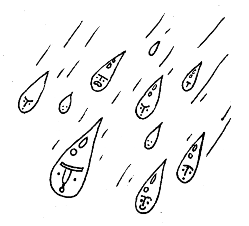
\includegraphics[scale=0.5]{16}}
\end{figure}
\end{SBSection*}
\end{song}

%\twocolumn
\begin{song}{Двадцать дней}{}{Сказка}{Сказка}{}{}


Двадцать дн\Ch{Dm}{ей} – это смена без дня.\par
“Маловато”,– вам скажут друзь\Ch{Gm}{я,}\par
А вожатый отв\Ch{C}{ет}ит люб\Ch{F}{ой}:\par
Это ср\Ch{Gm}{ок} очень д\Ch{A}{аж}е больш\Ch{Dm}{ой!}\\
 

Припев:\par
\ttМожно з\Ch{Gm C}{а-а-а-а} него усп\Ch{Dm}{ет}ь,\par
\ttНаприм\Ch{Gm}{ер,} полмилли\Ch{A}{он}а песен сп\Ch{Dm}{еть,}\par
\ttНо не к\Ch{Gm}{ажд}ый ведь поймет,\par
\ttКак так быстро раскрыв\Ch{A}{ат}ься может р\Ch{Dm}{от!}\\


Для полярника это не срок:\par
Не успеет просохнуть носок.\par
А вожатый успеет подряд \par
Вымыть, высушить сотню ребят!\\

Припев:\par
\ttВедь за смену, как за год \par
\ttСтолько разных мелочей произойдет,\par
\ttНо пока что нам везет,\par
\ttНас начальство для чего-то бережёт.\\


\newpage
Хоть и длинными кажутся дни,\par
Но как миг пролетели они.\par
Будешь долго потом вспоминать,\par
Как в отбой ты любил слово «СПАААТЬ!!!»\\

Припев:\par
\tt          	— Говорят за двадцать дней \par
\tt          	Все узнаешь о напарнице своей…\par
\tt          	— Только это ерунда,\par
\tt          	Обо всем ты не узнаешь никогда!\\

Смена вряд ли даст ответ:\par
Ты нашел свое призванье или нет.\par
Так что надо продолжать,\par
Двадцать раз по двадцать суток отсчитать!\\

\begin{SBSection*}
\begin{figure}[b!]
\center{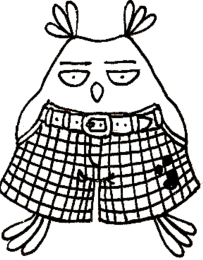
\includegraphics[scale=0.5]{17}}
\end{figure}
\end{SBSection*}

\end{song}

%\twocolumn
\begin{song}{Непогода}{}{Павел Смеян}{Павел Смеян}{}{}

\Ch{D}{Из}менения в природе \Ch{G}{пр}оисходят г\Ch{A}{од} от года,\par
\Ch{D}{Не}погода нынче в моде,\Ch{G}{} н\Ch{F#7}{епог}ода, непогода,\par
\Ch{}Hm{Слов}но из вод\Ch{F#7}{опро}вода \Ch{D7}{ль}ёт на нас с неб\Ch{G}{ес} во\Ch{Hm}{да…}\par
Полг\Ch{G}{од}а плох\Ch{A}{ая} пог\Ch{D}{од}а, \Ch{Hm}{пол}го\Ch{G}{да} — совс\Ch{A}{ем} нику\Ch{D}{да}.\par
Полг\Ch{G}{од}а плох\Ch{A}{ая} пог\Ch{D}{од}а, \Ch{Hm}{пол}го\Ch{G}{да} — сов\Ch{F#7}{сем} нику\Ch{Hm}{да.}\\


\SBChorusTagg:\par
\ttНикуда, нику\Ch{Em}{да н}ельз\Ch{A}{я} укр\Ch{D}{ы}ться н\Ch{Hm}{ам,}\par
\ttНо откладывать ж\Ch{Em}{изнь} ни\Ch{A}{как} нель\Ch{D}{зя}, \Ch{Hm}{}\par
\ttНикуда, нику\Ch{Em}{да, н}о зн\Ch{A}{ай}, что гд\Ch{D}{е}-то т\Ch{Hm}{ам}\par
\ttКто-то ищет теб\Ch{G}{я} сре\Ch{F#7}{ди д}ожд\Ch{Hm}{я.} \Ch{A}{}\\


Грома грозные раскаты от заката до восхода,\par
За грехи людские плата — непогода, непогода,\par
Не ангина, не простуда, посерьёзнее беда.\par
Полгода плохая погода, полгода — совсем никуда\par,
Полгода плохая погода, полгода — совсем никуда.\\\


\SBChorusTagg:\par
\ttНикуда, нику\Ch{Em}{да н}ельз\Ch{A}{я} укр\Ch{D}{ы}ться н\Ch{Hm}{ам,}\par
\ttНо откладывать ж\Ch{Em}{изнь} ни\Ch{A}{как} нель\Ch{D}{зя}, \Ch{Hm}{}\par
\ttНикуда, нику\Ch{Em}{да, н}о зн\Ch{A}{ай}, что гд\Ch{D}{е}-то т\Ch{Hm}{ам}\par
\ttКто-то ищет теб\Ch{G}{я} сре\Ch{F#7}{ди д}ожд\Ch{Hm}{я.} \Ch{A}{}\\


\end{song}

%\twocolumn
\begin{song}{Птенцы}{}{Сказка}{Сказка}{}{}

\Ch{Am}{}  \Ch{Am}{}

Как птенцы из гнез\Ch{Dm}{да} мы \Ch{E}{вы}па\Ch{Am}{ли.}\par
Ты не бойся при\Ch{Dm}{хо}да \Ch{G}{ве}че\Ch{C}{ра.}\par
Под та\Ch{A7}{ки}ми боль\Ch{F}{ши}ми \Ch{A7}{ли}па\Ch{Dm}{ми}\par
Нам с то\Ch{F}{бой} опа\Ch{Dm}{сать}ся \Ch{F}{не}\Ch{E}{че}\Ch{Am}{го.}\\
 
Под такими густыми звёздами -\par
Разве их не для нас рассыпали,\par
Мы не против гнездовья - просто мы\par
Из него ненароком выпали.\\

Это только вначале кажется,\par
Что без дома прожить нельзя никак,\par
Что важней пропитанья кашица,\par
Чем огромные звёзды на небе.\\

Ты не бойся ни тьмы, ни холода.\par
Будет день и найдётся пища нам,\par
Мы ещё пролетим над городом\par
На крыле до небес возвышенном.\\

Пролетим ещё - эка невидаль\par
Над Нью-Йорком, Парижем, Триполи\par
И над липой, откуда некогда,\par
Как птенцы из гнезда мы выпали.\\

Как птенцы из гнезда мы выпали.\par
Ты не бойся прихода вечера.\par
Под такими большими липами\par
Нам с тобой опасаться нечего.\\

\end{song}

%\twocolumn
\begin{song}{Продавец зонтиков}{}{Веня Дркин}{Веня Дркин}{}{}

\Ch{Am}{Город} этот выдумал о\Ch{Dm}{дин} художник,\par
\Ch{G}{Лю}ди в нем не знали, что та\Ch{C}{ко}е дождик.\par
\Ch{A7}{Про}сто не слыхали, что та\Ch{Dm}{ко}е зонтик –\par
\Ch{E7}{Вот} такие люди жили в \Ch{Am}{го}роде том.\par
И один чудак, в старый плащ одетый,\par
Продавал там зонтики зимой и летом,\par
Продавал там зонтики зимой и летом\par
И такую песенку он напевал:\\

\SBChorusTagg:\par
\tt“Господа, купите зонтик.\par
\ttБелый зонтик, красный зонтик,\par
\ttЖелтый зонтик, синий зонтик –\par
\ttМожет пригодится вам.”\\

Были домики у них из пластилина,\par
Из пустых коробочек автомашины,\par
И, не опасаясь никакой ангины,\par
Маленькие люди жили в городе том.\par
Маленькие были у людей заботы:\par
Шли они в кино или в театр с работы.\par
Вечером в подъезде целовался кто-то.\par
Все шутили и смеялись над стариком.\\


\SBChorusTagg.\\

\newpage

Маленькое небо как-то вдруг намокло,\par
В крошечных домишках задрожали стекла,\par
И огромный дождь пошел гулять по крышам,\par
Сразу все схватили насморк в городе том.\par
Вспомнили тут люди о торговце старом,\par
Кинулись искать его по всем базарам,\par
Но исчез торговец со своим товаром.\par
Только песенка осталась в память о нем:\\

\SBChorusTagg.\par

\begin{SBSection*}
\begin{figure}[b!]
\center{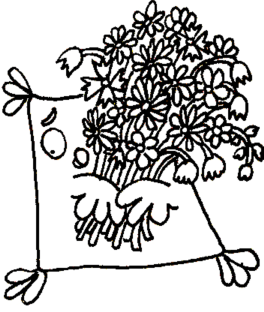
\includegraphics[scale=0.5]{15}}
\end{figure}
\end{SBSection*}

\end{song}

%\twocolumn
\begin{song}{Белая гвардия}{}{Белая гвардия}{Белая гвардия}{}{}

Проигрыш: (2 раза)\par 
\Ch{Am}{} \Ch{D}{} \Ch{G}{} \Ch{C}{} \Ch{Am}{} \Ch{H7}{} \Ch{Em}\\

\Ch{Em}{Белая} гвардия, белый снег,\par
\Ch{Am7}{Белая} музыка революций.\par
\Ch{D7}{Белая} женщина, нервный смех,\par
\Ch{G}{Белого} платья слегка коснуться.\par
 
Белой рукой распахнуть окно,\par
Белого света в нем не видя.\par
Белое выпить до дна вино,\par
В красную улицу в белом выйти.\\

Припев:\par
\ttКог\Ch{Em}{да} ты вернешься,\par
\ttВсе будет и\Ch{Am}{на}че, и нам бы узнать друг друга,\par
\ttКог\Ch{D7}{да} ты вернешься,\par
\ttА я не же\Ch{G}{на} и даже \Ch{H7}{не} подруга.\par
\ttКог\Ch{C}{да} ты вернешься,\par
\ttКо мне, так без\Ch{Am}{ум}но тебя любившей в прошлом,\par
\tt\Ch{D7}{Ко}гда ты вернешься -\par
\ttУвидишь, что ж\Ch{G}{ре}бий давно и не \Ch{E7}{нами} брошен.\\

Проигрыш.\\
 
\newpage
Сизые сумерки прошлых лет\par
Робко крадутся по переулкам.\par
В этом окне еле брезжит свет,\par
Ноты истрепаны, звуки гулки.\par
Тонкие пальцы срывают аккорд...\par
Нам не простят безрассудного дара.\par
Бьются в решетку стальных ворот\par
Пять океанов земного шара.\\

Припев. \par
Проигрыш.\\
 
Красный трамвай простучал в ночи,\par
Красный закат догорел в бокале,\par
Красные-красные кумачи\par
С красных деревьев на землю упали.\par
Я не ждала тебя в октябре,\par
Виделись сны, я листала сонник:\par
Красные лошади на заре\par
Били копытами о подоконник.\\

Припев:\par
\ttКогда ты вернешься,\par
\ttВсе будет иначе, и нам бы узнать друг друга,\par
\ttКогда ты вернешься,\par
\ttА я не жена и даже не подруга.\par
\ttКогда ты вернешься,\par
\ttВернешься в наш город обетованный,\par
\ttКогда ты вернешься -\par
\ttТакой невозможный и такой желанный?\\

Проигрыш.\par

\end{song}

%\twocolumn
\begin{song}{Перевал}{}{Песни у костра}{Песни у костра}{}{}


\Ch{Am}{Про}сто нечего нам \Ch{Dm}{боль}ше терять\par
\Ch{E}{Всё} нам вспомнится на \Ch{Am}{Страшном} суде.\par
Эта ночь легла, как \Ch{Dm}{тот} перевал,\par
\Ch{G}{За} которым испол\Ch{C}{нень}е надежд.\par
\Ch{A7}{Про}сто прожитое—про\Ch{Dm}{жи}то зря, \Ch{G}{}\par
Но не в этом, пони\Ch{C}{мае}шь ли, соль… \Ch{Am}{}\par
Слышишь, падают дож\Ch{Dm}{ди} октября.\par
\Ch{E}{Ви}дишь, старый дом сто\Ch{Am}{ит} средь лесов.\\

Мы затопим в доме печь, в доме печь,\par
Мы гитару позовем со стены.\par
Просто нечего нам больше беречь,\par
Ведь за нами все мосты сожжены.\par
Все мосты, все перекрёстки дорог,\par
Все прошёптанные тайны в ночи.\par
Каждый сделал все, что смог, все, что смог,\par
Мы об этом помолчим, помолчим.\\


И луна взойдет заплывшей свечой,\par
Ставни скрипнут  на ветру, на ветру.\par
Ах, как я тебя люблю горячо,\par
Это годы не сотрут, не сотрут.\par
Мы оставшихся друзей соберем,\par
Мы набьем картошкой старый рюкзак,\par
Люди спросят: "Что за шум, что за гам?"\par
Мы ответим: "Просто так,  просто так”...\\

\newpage

    Просто так идут дожди в октябре,\par
    И потеряны от счастья ключи.\par
    Это всё, конечно, мне, конечно, мне,\par
    Но об этом помолчим, помолчим.\par
    Просто прожитое—прожито зря,\par
    Но не в этом, понимаешь ли, соль…\par
    Слышишь, падают дожди октября.\par
    Видишь, старый дом стоит средь лесов.\par


\begin{SBSection*}
\begin{figure}[b!]
\center{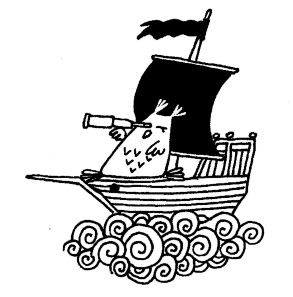
\includegraphics[scale=0.5]{22}}
\end{figure}
\end{SBSection*}

\end{song}

%\twocolumn
\begin{song}{Ленинградская (Все расстояния)}{}{Песни у костра}{Песни у костра}{}{}

\Ch{Am}{Все} расстоянья когда-нибудь в круг замы\Ch{E}{ка}ются,\par
\Ch{E}{Все} из разлук обязательно \Ch{E7}{встре}чей кон\Ch{Am}{ча}ются;\par
Должны про\Ch{Dm}{плыть} вокруг Зем\Ch{G}{ли,}\par
Вернуться в \Ch{C}{га}вань кораб\Ch{F}{ли,}\par   
Все поез\Ch{Dm}{да} в свои вер\Ch{E}{нуть}ся горо\Ch{Am}{да.}\\
 
Шумный вокзал то встречает друзей , то прощается,\par
Мы расстаемся, но снова назад возвращаемся -\par
Чтоб снова встать в огромный круг,\par
И снова знать, что рядом друг ,\par
И песни петь, чтоб больше не было разлук.\\
 
Все расстоянья когда-нибудь в круг замыкаются,\par
Все из разлук обязательно встречей кончаются;\par
И через год, и через пять,\par
Мы с вами встретимся опять,\par
Ничто не сможет нашей дружбе помешать.\par

\end{song}

%\twocolumn
\begin{song}{Десять капель}{}{Танцы Минус}{Танцы Минус}{}{}

Проигрыш: (2 раза)\par 
\Ch{C}{} \Ch{E}{} \Ch{Am}{} \Ch{F}{} \Ch{C}{} \Ch{E}{} \Ch{Am}{} \Ch{F}{}

\Ch{C}{Де}сять капель дож\Ch{E}{дя} у тебя на пле\Ch{Am}{че}\par
Ты забыла свой \Ch{F}{зонт,} ты спешила ко \Ch{C}{мне.}\par
Десять капель дож\Ch{E}{дя} на плече у те\Ch{Am}{бя,}\par
Десять капель люб\Ch{F}{ви,} десять капель ог\Ch{C}{ня}\\

Припев:\\(Три первых слова в припеве дублируются вторым голосом)\par
\tt\Ch{C}{Т}воя\Ch{E}{} ладо\Ch{Am}{нь} горит\Ch{F}{} в моих руках\par
\tt\Ch{C}{Л}юбви\Ch{E}{ }пож\Ch{Am}{ар} горит в тво\Ch{F}{их} глазах\\

Проигрыш.\\

Время делает шаг, время делает круг\par
Мы забудем друзей, мы забудем подруг\par
Просто выпьем вина из любви и огня\par
Десять капель меня, десять капель тебя\\

Припев.\\

Голос твой в тишине околдует меня\par
Ярким жарким огнем стану я до утра\par
Ты прикажешь гори, и я вспыхну любя\par
В этом пламени ты, в этом пламени я.\par

\end{song}

%\twocolumn
\begin{song}{Макет}{}{Песни у костра}{Сказка}{}{}
sadfsfthanks,\par
\begin{SBOpGroup}
asdas\
\end{SBOpGroup}
\begin{SBSection*}fdf\end{SBSection*}
\begin{SBVerse*}\end{SBVerse*}
\begin{SBChorus*}\end{SBChorus*}

\begin{SBOccurs}{23}
dsf
\end{SBOccurs}

\begin{SBSection*}
\begin{figure}[b!]
\center{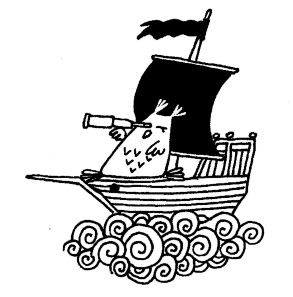
\includegraphics[scale=0.5]{22}}
\end{figure}
\end{SBSection*}
\end{song}

\mainmatter

\renewcommand{\footrulewidth}{0.0pt}
\renewcommand{\item}{\par\hangindent=40pt}
\renewcommand{\subitem}{\par\hangindent=40pt \hspace*{20pt}}
\renewcommand{\subsubitem}{\par\hangindent=40pt \hspace*{30pt}}

\newpage
\raggedright\input{/home/p_a/git/ska3ka/ps.adx}

\centering\includegraphics[scale=0.5]{10}

\newpage
\raggedright\input{/home/p_a/git/ska3ka/ps.tdx}

\centering\includegraphics[scale=0.5]{11}

\end{document}


\centering\includegraphics[scale=0.5]{11}

\end{document}


\centering\includegraphics[scale=0.5]{11}

\end{document}


\centering\includegraphics[scale=0.5]{10}

\newpage
\raggedright%\documentclass[a5paper,11pt]{book}
%\usepackage{fancyhdr}
%\usepackage[chordbk]{songbook}
%
%\usepackage[T2A]{fontenc}
%\usepackage[utf8]{inputenc}
%\usepackage[russian]{babel}
%
%\title{A Church Songbook}
%\author{}
%\date{Revised:  \RevDate}
%
%\newcommand{\RelDate}{13 November'19}
%\newcommand{\RevDate}{\today}

\documentclass[11pt,a5paper]{book}
\usepackage[a5paper]{geometry}
\usepackage[chordbk]{songbook}
\usepackage[T2A]{fontenc}
\usepackage[utf8]{inputenc}
\usepackage[russian]{babel}
\usepackage{cmap} % для работы поиска кириллицы в pdf

%\usepackage{amsmath,amsthm,amssymb}
%\usepackage{mathtext}


\usepackage[pdftex]{graphicx}
\usepackage{lscape}
%\usepackage{vmargin}
\usepackage{textcomp}
\usepackage{setspace}
%\usepackage{marvosym}
\usepackage{gensymb} %%%for \micro tag
\usepackage{upgreek} %%% \upmu
\usepackage{tipa}
\usepackage{phonetic}
%\usepackage[greek,english]{babel}
\usepackage{threeparttable}
\usepackage{multirow}
\usepackage{harvard}
\usepackage{longtable}
\renewcommand{\sectionmark}[1]{\markright{#1}}
\renewcommand{\chaptermark}[1]{\markboth{#1}{}}
\addto\captionsenglish{\renewcommand{\bibname}{References}}
\usepackage{latexsym,fancyhdr}

\newcommand{\RelDate}{26 Апреля'1984}
\newcommand{\RevDate}{\today}

%%%
% C.C.L.I. license number definition; for copyright licensing info.
% One of these macros will be manually inserted into the {CpyRt}
% parameter of the {song} environment.
%
%       \CCLInumber - The actual copyright license number.  Don't
%               insert this command in the {CpyRt} parameter, use one
%               of the others.
%       \CCLIed - Indicates a song falls under our CCLI license.
%       \NotCCLIed - Indicates a song doesn't fall under our CCLI
%               license.  Public Domain songs fall into this category.
%       \PGranted - We have received specific permission from the
%               copyright holder to use this song.
%       \PPending - We are in the process of obtaining permission to
%               use this song.
%%%
\newcommand{\CCLInumber}{Your CCLI Number}
\newcommand{\CCLIed}{{\CpyRtInfoFont (CCLI \CCLInumber)}}
\newcommand{\NotCCLIed}{\relax}
\newcommand{\PGranted}{\relax}
\newcommand{\PPending}{{\CpyRtInfoFont (Permission Pending)}}

%%%
% Title page information.
%%%
\title{ Сказочный песенник}
\author{}
\date{Созданно:  \RevDate}


%%%
% Define fonts to use in the headers and footers of the songbook.
%%%
\newcommand{\LHeadFont}{\normalsize}            % = cmr12  at 12pt
\newcommand{\CHeadFont}{\normalsize\rm}         % = cmr12  at 12pt
\newcommand{\RHeadFont}{\normalsize}            % = cmr12  at 12pt
\newcommand{\LFootFont}{\scriptsize}            % = cmr8   at  8pt
\newcommand{\CFootFont}{\tiny\myTinySF}         % = cmss8  at  8pt
\newcommand{\RFootFont}{\scriptsize}            % = cmr8   at  8pt

%%%
% Turn on and define fancy page heading/footing definition.
%%%
\pagestyle{fancy}

\ifChordBk
  % It's a words & chords songbook...
%  \addtolength{\headwidth}{\marginparsep}
%  \addtolength{\headwidth}{\marginparwidth}
  \renewcommand{\headrulewidth}{0.0pt}
  \renewcommand{\footrulewidth}{0.0pt}
%  \fancyhead[LE,RO]{\LHeadFont\emph{\leftmark\/}}
%  \fancyhead[CE,CO]{\CHeadFont\thepage}
  \fancyhead[RE,LO]{~}
\else\ifOverhead
  % It's an overhead...
  \renewcommand{\footrulewidth}{0pt}
  \renewcommand{\headrulewidth}{0pt}
  \fancyhead[LE,RO]{}
  \fancyhead[CE,CO]{}
  \fancyhead[RE,LO]{}
\else\ifWordBk
  % It's a words only songbook...
  \addtolength{\headwidth}{\marginparsep}
  \addtolength{\headwidth}{\marginparwidth}
  \renewcommand{\headrulewidth}{0.0pt}
  \renewcommand{\footrulewidth}{0.0pt}
  \fancyhead[LE,RO]{\LHeadFont A Church Songbook}
  \fancyhead[CE,CO]{\CHeadFont\thepage}
  \fancyhead[RE,LO]{\RHeadFont\RelDate}
\fi\fi\fi

%\fancyfoot[LE,RO]{\LFootFont Property of The Church}
%\ifSongEject
%  \fancyfoot[CE,CO]{\CFootFont \RevDate}
%\else
%  \fancyfoot[CE,CO]{\CFootFont}
%\fi
%\fancyfoot[RE,LO]{\RFootFont Material used by permission.}

%%%
% Turn on/off index-file generation.  Uncomment the \makeindex line to
% turn index generation on;  comment it out to turn index generation
% off.
%%%
\makeTitleIndex         %% Title and First Line Index.
\makeTitleContents      %% Table of Contents.
\makeKeyIndex           %% Index of song by key.
\graphicspath{{img/}} % папка с картинками
\DeclareGraphicsExtensions{.pdf,.png,.jpg} % форматы, которые будем считать картинками

%\newenvironment{song}[7][Y]{
%% Comment markers to negate
%\if#1Y\ExcludeSongfalse\else\ExcludeSongtrue\fi% the newline.
%\ifPrintAllSongs\ExcludeSongfalse\fi
%\SongMarkboth{\relax}{\relax}
%\SBinSongEnvtrue
%\renewcommand{\SBinSongEnv}{\True}
%\ifWordsOnly
%	\setlength{\parindent}{0pt}
%\fi

%%%
% Redefine fonts from SongBook style that I don't like.
%%%
\font\myTinySF=cmss8 at 8pt
\renewcommand{\CpyRtInfoFont}{\tiny\myTinySF}


%
%\font\myTinySF=cmss8    at  8pt
%\font\myHugeSF=cmssbx10 at 25pt
%\renewcommand{\CpyRtInfoFont}{\tiny\myTinySF}
%\newcommand{\myTitleFont}{\Huge\myHugeSF}
%\newcommand{\mySubTitleFont}{\large\sf}

%%% Работа с русским языком
%\usepackage[no-math]{fontspec}      %% подготавливает загрузку шрифтов Open Type, True Type и др.
%\defaultfontfeatures{Ligatures={TeX},Renderer=Basic}  %% свойства шрифтов по умолчанию
%\setmainfont[Ligatures={TeX,Historic}]{Times New Roman} %% задаёт основной шрифт документа
%\setsansfont{Helvetica Neue}                    %% задаёт шрифт без засечек

%\newfontfamily{\allods}{AllodsWest}

\newcommand{\SBPubDomm}{~}
\renewcommand{\CpyRt}[3][Y]{%
\if#1Y\begin{center}\fi
\if\blank{#2}%
\if\blank{#3}%
{\CpyRtFont\copyright \SBUnknownTag{} \CpyRtInfoFont}%
\else
{\CpyRtFont\copyright \SBUnknownTag{} \CpyRtInfoFont #3}%
\fi%
\else%
\ifthenelse{\equal{#2}{\SBPubDomm}}
{%then
{\CpyRtFont #2 \CpyRtInfoFont #3}%
}{%else
{\CpyRtFont #2 \CpyRtInfoFont #3}%
}%fi
\fi%
\if#1Y\end{center}\fi
}


\newcommand{\SBUnknownTagg}{~}
\renewcommand{\WAndM}[2][Y]{~}
\renewcommand{\WAndM}[2][Y]{%
\if#1Y\begin{center}\fi
\if\blank{#2}%
{\SBUnknownTagg}%
\else
{~}%
\fi
\if#1Y\end{center}\fi
}

\renewcommand{\STitle}[3][Y]{%
\setcounter{SBVerseCnt}{0}%
\setcounter{SBSectionCnt}{0}%
\ifExcludeSong\relax%
	\else\keyIndex{{\protect\sbChord#3\protect\relax} -- #2}{\theSBSongCnt}\fi%
	\vspace{\SpaceAboveSTitle}%
\if#1Y\begin{center}\fi
	{}{\STitleFont\LARGE #2}%
	\ifWordsOnly\relax\else\fi%
	\if#1Y\end{center}\fi
\STitleMarkboth{#2}{\relax}%
}


%\renewenvironment{SBOpGroup}{%
%	\sbSetsbBaselineSkipAmt%
%	\bgroup%
%	\begin{list}{\hbox{}}
%	  {\setlength {\leftmargin}
%		{\HangAmt}
%		\setlength{\itemindent}
%			{-\HangAmt}
%		\setlength{\listparindent}{-\HangAmt}
%		\setlength{\topsep}{0pt}
%		\setlength{\parsep}{0pt}
%		\setlength{\labelwidth}{0pt}
%		\setlength{\labelsep}{0pt}
%		\setlength{\baselineskip} {\sbBaselineSkipAmt}
%	}%\item}
%{\end{list}%
\newcommand{\SBChorusTagg}{Припев}
\renewenvironment{SBChorus}{%
\sbSetsbBaselineSkipAmt%
\bgroup%
\SBChorusMarkright{\SBChorusTag}
\begin{list}{{\SBChorusTagFont\SBChorusTagg}}
{\setlength {\leftmargin}
{\LeftMarginSBChorus + \HangAmt}
\setlength{\itemindent}
{-\HangAmt}
\setlength{\listparindent}{-\HangAmt}
\setlength{\parsep}
{0pt}
\setlength{\baselineskip} {\sbBaselineSkipAmt}
}%
\item}
{\end{list}%
\egroup%
\SpaceAfterChorus%
}

\renewcommand{\tt}{\indent \indent}
%\renewcommand{\nt}{\noindent}


\usepackage{amsmath}

\makeArtistIndex
\makeTitleIndex         %% Title and First Line Index.
\makeTitleContents      %% Table of Contents.
\makeKeyIndex           %% Index of song by key.
%\usepackage{printallsongs}

\begin{document} 
\maketitle

\mainmatter


\begin{song}{Вожатский гимн}{}{Сказка}{Сказка}{}{}

По \Ch{Am}{ла}герю подъём, нас горн зовёт!\par
Забудь о том, что ночь была бес\Ch{C}{сон}ною\par
Смо\Ch{Dm}{чи} водою \Ch{G}{ве}ки воспа\Ch{C}{лён}\Ch{F}{ные}\par    
По\Ch{Dm}{вя}зывай свой \Ch{E}{галс}тук — и впе\Ch{Am (A7)}{рёд!}\par
Смо\Ch{Dm}{чи} водою \Ch{G}{ве}ки воспа\Ch{C}{лён}\Ch{F}{ные}\par    
По\Ch{Dm}{вя}зывай свой \Ch{E}{галс}тук — и впе\Ch{Am (A7)}{рёд!}\par

%	\begin{SBChorus*}
\ttНе\Ch{E}{про}сто воспитывать \Ch{Am}{но}вых людей,\par
\ttНу \Ch{E}{что} ж, это наша с то\Ch{Am}{бою} свя\Ch{A7}{ты}ня.\par
\ttМой \Ch{Dm}{друг}, нам до\Ch{G}{ве}рили \Ch{C}{ду}ши де\Ch{F}{тей},\par
\ttИх \Ch{Dm}{ра}достный \Ch{Am}{смех} нам на\Ch{E}{гра}да от\Ch{Am}{ны}не.\par
\ttМой \Ch{Dm}{друг}, нам до\Ch{G}{ве}рили \Ch{C}{ду}ши де\Ch{F}{тей},\par
\ttИх \Ch{Dm}{ра}достный \Ch{Am}{смех} нам на\Ch{E}{гра}да от\Ch{Am}{ны}не.\\
%\end{SBChorus*}

Отбой, засыпает детвора.\par
Взгляни на их улыбки полусонные,\par
Пускай им снятся острова зелёные,\par
А нам опять работать до утра!\par
Пускай им снятся острова зелёные,\par
А нам опять работать до утра!\par

\tt И пусть от бессилья затихнешь не раз,\par
\ttИ голос усталый до хрипа натружен,\par
\ttПусть будут умней и счастливее нас\par
\ttТе дети, в которых вложили мы души!\par
\ttПусть будут умней и счастливее нас\par
\ttТе дети, в которых вложили мы души!

\end{song}

\begin{song}{Сказка в неглиже}{}{Сказка}{Сказка}{}{}

Есть у \Ch{C}{каж}дого добрая сказка в ду\Ch{F}{ше,}\par 
Надо \Ch{G}{толь}ко прочесть этой сказки стра\Ch{C}{ни}цы.\par
В тиши\Ch{C}{не}, разо\Ch{C7}{де}тая вся в негли\Ch{F}{же,}\par
Пусть на\Ch{G}{ве}ки она, пусть на\Ch{F}{ве}ки она сохра\Ch{C}{ни}тся. \Ch{C7}{ }\par 
В тиши\Ch{F}{не,} разо\Ch{G}{де}тая вся в негли\Ch{C}{же,} \Ch{Am}{}\par
Пусть на\Ch{F}{ве}ки она, пусть на\Ch{G}{ве}ки она сохра\Ch{C}{ни}тся.\\


\ttЭту сказку пред другом раскрыть поспеши,\par
\ttА врагу не спеши эту сказку поведать.\par
\ttПусть растут и читают ее малыши.\par
\ttБудь добрей, и тебя минут всякие беды.\par
\ttПусть растут и читают ее малыши.\par
\ttБудь добрей, и тебя минут всякие беды.\\


\Ch{C7}{}Будет \Ch{F}{мно}го распутий, \Ch{G}{до}рог и тре\Ch{C}{вог.}\Ch{Am}{}\par
На вис\Ch{F}{ки} твои ляжет \Ch{G}{не}тающий \Ch{C}{ин}ей, \Ch{C7}{}\par
И пой\Ch{F}{мёшь,} научившись чи\Ch{G}{тать} между \Ch{C}{строк:} \Ch{Am}{}\par
Даже \Ch{F}{гнус}ный злодей \Ch{G}{в} этой сказке не\Ch{C}{ви}нен. \Ch{C7}{}\par
И пой\Ch{F}{мёшь,} научившись чи\Ch{G}{тать} между ст\Ch{C}{рок:} \Ch{A}{}\par
Даже \Ch{F}{гнус}ный злодей \Ch{G}{в} этой сказке не\Ch{C}{ви}нен.\\

\Ch{C}{} \Ch{G}{} \Ch{F}{} \Ch{G}{} \Ch{C}{} \Ch{C7}{}\par
\Ch{C}{} \Ch{G}{} \Ch{F}{} \Ch{G}{} \Ch{C}{}
\end{song}

%\twocolumn
\begin{song}{Вожатский марш}{}{Сказка}{Сказка}{}{}

Есть на\Ch{Am}{род} у нас весёлый,\par
Самой \Ch{C}{луч}шей в мире пробы,\par
Песни \Ch{G}{петь} всегда мас\Ch{C}{так.}\Ch{A7}{}\par
Он всег\Ch{Dm}{да} всего добьётся,\par
Он Вожа\Ch{Am}{ты}ми зовётся,\par
\Ch{E}{Так} и только \Ch{Am (A7)}{так!}\par
Он всег\Ch{Dm}{да} всего добьётся,\par
Он Во\Ch{Am}{жа}тыми зовётся,\par
\Ch{E}{Так} и только \Ch{Am (A7)}{так!}\\

Домосед привязан к дому\par
И по случаю такому,\par
Он из дома — ни на шаг!\par
А вожатый — он в дороге,\par
Он готов в огонь и в воду,\par
Так и только так!\par
А вожатый — он в дороге,\par
Он готов в огонь и в воду,\par
Так и только так!\\
\newpage
Жадный денежки считает,\par
Все считает и считает,\par
К пятаку кладет пятак.\par
А вожатый деньги тратит,\par
Не боясь, что их не хватит,\par
Так и только так!\par
А вожатый деньги тратит,\par
Не боясь, что их не хватит,\par
Так и только так!\\

Холостяк в любовь не верит,\par
Все не верит и не верит,\par
Потому что холостяк.\par
А вожатых не влюблённых\par
Не найдёшь определённо,\par
Так и только так!\par
А вожатых не влюблённых\par
Не найдёшь определённо,\par
Так и только так!\par

\begin{SBSection*}
\begin{figure}[b!]
\center{\includegraphics[scale=0.5]{16}}
\end{figure}
\end{SBSection*}
\end{song}

%\twocolumn
\begin{song}{Двадцать дней}{}{Сказка}{Сказка}{}{}


Двадцать дн\Ch{Dm}{ей} – это смена без дня.\par
“Маловато”,– вам скажут друзь\Ch{Gm}{я,}\par
А вожатый отв\Ch{C}{ет}ит люб\Ch{F}{ой}:\par
Это ср\Ch{Gm}{ок} очень д\Ch{A}{аж}е больш\Ch{Dm}{ой!}\\
 

Припев:\par
\ttМожно з\Ch{Gm C}{а-а-а-а} него усп\Ch{Dm}{ет}ь,\par
\ttНаприм\Ch{Gm}{ер,} полмилли\Ch{A}{он}а песен сп\Ch{Dm}{еть,}\par
\ttНо не к\Ch{Gm}{ажд}ый ведь поймет,\par
\ttКак так быстро раскрыв\Ch{A}{ат}ься может р\Ch{Dm}{от!}\\


Для полярника это не срок:\par
Не успеет просохнуть носок.\par
А вожатый успеет подряд \par
Вымыть, высушить сотню ребят!\\

Припев:\par
\ttВедь за смену, как за год \par
\ttСтолько разных мелочей произойдет,\par
\ttНо пока что нам везет,\par
\ttНас начальство для чего-то бережёт.\\


\newpage
Хоть и длинными кажутся дни,\par
Но как миг пролетели они.\par
Будешь долго потом вспоминать,\par
Как в отбой ты любил слово «СПАААТЬ!!!»\\

Припев:\par
\tt          	— Говорят за двадцать дней \par
\tt          	Все узнаешь о напарнице своей…\par
\tt          	— Только это ерунда,\par
\tt          	Обо всем ты не узнаешь никогда!\\

Смена вряд ли даст ответ:\par
Ты нашел свое призванье или нет.\par
Так что надо продолжать,\par
Двадцать раз по двадцать суток отсчитать!\\

\begin{SBSection*}
\begin{figure}[b!]
\center{\includegraphics[scale=0.5]{17}}
\end{figure}
\end{SBSection*}

\end{song}

%\twocolumn
\begin{song}{Непогода}{}{Павел Смеян}{Павел Смеян}{}{}

\Ch{D}{Из}менения в природе \Ch{G}{пр}оисходят г\Ch{A}{од} от года,\par
\Ch{D}{Не}погода нынче в моде,\Ch{G}{} н\Ch{F#7}{епог}ода, непогода,\par
\Ch{}Hm{Слов}но из вод\Ch{F#7}{опро}вода \Ch{D7}{ль}ёт на нас с неб\Ch{G}{ес} во\Ch{Hm}{да…}\par
Полг\Ch{G}{од}а плох\Ch{A}{ая} пог\Ch{D}{од}а, \Ch{Hm}{пол}го\Ch{G}{да} — совс\Ch{A}{ем} нику\Ch{D}{да}.\par
Полг\Ch{G}{од}а плох\Ch{A}{ая} пог\Ch{D}{од}а, \Ch{Hm}{пол}го\Ch{G}{да} — сов\Ch{F#7}{сем} нику\Ch{Hm}{да.}\\


\SBChorusTagg:\par
\ttНикуда, нику\Ch{Em}{да н}ельз\Ch{A}{я} укр\Ch{D}{ы}ться н\Ch{Hm}{ам,}\par
\ttНо откладывать ж\Ch{Em}{изнь} ни\Ch{A}{как} нель\Ch{D}{зя}, \Ch{Hm}{}\par
\ttНикуда, нику\Ch{Em}{да, н}о зн\Ch{A}{ай}, что гд\Ch{D}{е}-то т\Ch{Hm}{ам}\par
\ttКто-то ищет теб\Ch{G}{я} сре\Ch{F#7}{ди д}ожд\Ch{Hm}{я.} \Ch{A}{}\\


Грома грозные раскаты от заката до восхода,\par
За грехи людские плата — непогода, непогода,\par
Не ангина, не простуда, посерьёзнее беда.\par
Полгода плохая погода, полгода — совсем никуда\par,
Полгода плохая погода, полгода — совсем никуда.\\\


\SBChorusTagg:\par
\ttНикуда, нику\Ch{Em}{да н}ельз\Ch{A}{я} укр\Ch{D}{ы}ться н\Ch{Hm}{ам,}\par
\ttНо откладывать ж\Ch{Em}{изнь} ни\Ch{A}{как} нель\Ch{D}{зя}, \Ch{Hm}{}\par
\ttНикуда, нику\Ch{Em}{да, н}о зн\Ch{A}{ай}, что гд\Ch{D}{е}-то т\Ch{Hm}{ам}\par
\ttКто-то ищет теб\Ch{G}{я} сре\Ch{F#7}{ди д}ожд\Ch{Hm}{я.} \Ch{A}{}\\


\end{song}

%\twocolumn
\begin{song}{Птенцы}{}{Сказка}{Сказка}{}{}

\Ch{Am}{}  \Ch{Am}{}

Как птенцы из гнез\Ch{Dm}{да} мы \Ch{E}{вы}па\Ch{Am}{ли.}\par
Ты не бойся при\Ch{Dm}{хо}да \Ch{G}{ве}че\Ch{C}{ра.}\par
Под та\Ch{A7}{ки}ми боль\Ch{F}{ши}ми \Ch{A7}{ли}па\Ch{Dm}{ми}\par
Нам с то\Ch{F}{бой} опа\Ch{Dm}{сать}ся \Ch{F}{не}\Ch{E}{че}\Ch{Am}{го.}\\
 
Под такими густыми звёздами -\par
Разве их не для нас рассыпали,\par
Мы не против гнездовья - просто мы\par
Из него ненароком выпали.\\

Это только вначале кажется,\par
Что без дома прожить нельзя никак,\par
Что важней пропитанья кашица,\par
Чем огромные звёзды на небе.\\

Ты не бойся ни тьмы, ни холода.\par
Будет день и найдётся пища нам,\par
Мы ещё пролетим над городом\par
На крыле до небес возвышенном.\\

Пролетим ещё - эка невидаль\par
Над Нью-Йорком, Парижем, Триполи\par
И над липой, откуда некогда,\par
Как птенцы из гнезда мы выпали.\\

Как птенцы из гнезда мы выпали.\par
Ты не бойся прихода вечера.\par
Под такими большими липами\par
Нам с тобой опасаться нечего.\\

\end{song}

%\twocolumn
\begin{song}{Продавец зонтиков}{}{Веня Дркин}{Веня Дркин}{}{}

\Ch{Am}{Город} этот выдумал о\Ch{Dm}{дин} художник,\par
\Ch{G}{Лю}ди в нем не знали, что та\Ch{C}{ко}е дождик.\par
\Ch{A7}{Про}сто не слыхали, что та\Ch{Dm}{ко}е зонтик –\par
\Ch{E7}{Вот} такие люди жили в \Ch{Am}{го}роде том.\par
И один чудак, в старый плащ одетый,\par
Продавал там зонтики зимой и летом,\par
Продавал там зонтики зимой и летом\par
И такую песенку он напевал:\\

\SBChorusTagg:\par
\tt“Господа, купите зонтик.\par
\ttБелый зонтик, красный зонтик,\par
\ttЖелтый зонтик, синий зонтик –\par
\ttМожет пригодится вам.”\\

Были домики у них из пластилина,\par
Из пустых коробочек автомашины,\par
И, не опасаясь никакой ангины,\par
Маленькие люди жили в городе том.\par
Маленькие были у людей заботы:\par
Шли они в кино или в театр с работы.\par
Вечером в подъезде целовался кто-то.\par
Все шутили и смеялись над стариком.\\


\SBChorusTagg.\\

\newpage

Маленькое небо как-то вдруг намокло,\par
В крошечных домишках задрожали стекла,\par
И огромный дождь пошел гулять по крышам,\par
Сразу все схватили насморк в городе том.\par
Вспомнили тут люди о торговце старом,\par
Кинулись искать его по всем базарам,\par
Но исчез торговец со своим товаром.\par
Только песенка осталась в память о нем:\\

\SBChorusTagg.\par

\begin{SBSection*}
\begin{figure}[b!]
\center{\includegraphics[scale=0.5]{15}}
\end{figure}
\end{SBSection*}

\end{song}

%\twocolumn
\begin{song}{Белая гвардия}{}{Белая гвардия}{Белая гвардия}{}{}

Проигрыш: (2 раза)\par 
\Ch{Am}{} \Ch{D}{} \Ch{G}{} \Ch{C}{} \Ch{Am}{} \Ch{H7}{} \Ch{Em}\\

\Ch{Em}{Белая} гвардия, белый снег,\par
\Ch{Am7}{Белая} музыка революций.\par
\Ch{D7}{Белая} женщина, нервный смех,\par
\Ch{G}{Белого} платья слегка коснуться.\par
 
Белой рукой распахнуть окно,\par
Белого света в нем не видя.\par
Белое выпить до дна вино,\par
В красную улицу в белом выйти.\\

Припев:\par
\ttКог\Ch{Em}{да} ты вернешься,\par
\ttВсе будет и\Ch{Am}{на}че, и нам бы узнать друг друга,\par
\ttКог\Ch{D7}{да} ты вернешься,\par
\ttА я не же\Ch{G}{на} и даже \Ch{H7}{не} подруга.\par
\ttКог\Ch{C}{да} ты вернешься,\par
\ttКо мне, так без\Ch{Am}{ум}но тебя любившей в прошлом,\par
\tt\Ch{D7}{Ко}гда ты вернешься -\par
\ttУвидишь, что ж\Ch{G}{ре}бий давно и не \Ch{E7}{нами} брошен.\\

Проигрыш.\\
 
\newpage
Сизые сумерки прошлых лет\par
Робко крадутся по переулкам.\par
В этом окне еле брезжит свет,\par
Ноты истрепаны, звуки гулки.\par
Тонкие пальцы срывают аккорд...\par
Нам не простят безрассудного дара.\par
Бьются в решетку стальных ворот\par
Пять океанов земного шара.\\

Припев. \par
Проигрыш.\\
 
Красный трамвай простучал в ночи,\par
Красный закат догорел в бокале,\par
Красные-красные кумачи\par
С красных деревьев на землю упали.\par
Я не ждала тебя в октябре,\par
Виделись сны, я листала сонник:\par
Красные лошади на заре\par
Били копытами о подоконник.\\

Припев:\par
\ttКогда ты вернешься,\par
\ttВсе будет иначе, и нам бы узнать друг друга,\par
\ttКогда ты вернешься,\par
\ttА я не жена и даже не подруга.\par
\ttКогда ты вернешься,\par
\ttВернешься в наш город обетованный,\par
\ttКогда ты вернешься -\par
\ttТакой невозможный и такой желанный?\\

Проигрыш.\par

\end{song}

%\twocolumn
\begin{song}{Перевал}{}{Песни у костра}{Песни у костра}{}{}


\Ch{Am}{Про}сто нечего нам \Ch{Dm}{боль}ше терять\par
\Ch{E}{Всё} нам вспомнится на \Ch{Am}{Страшном} суде.\par
Эта ночь легла, как \Ch{Dm}{тот} перевал,\par
\Ch{G}{За} которым испол\Ch{C}{нень}е надежд.\par
\Ch{A7}{Про}сто прожитое—про\Ch{Dm}{жи}то зря, \Ch{G}{}\par
Но не в этом, пони\Ch{C}{мае}шь ли, соль… \Ch{Am}{}\par
Слышишь, падают дож\Ch{Dm}{ди} октября.\par
\Ch{E}{Ви}дишь, старый дом сто\Ch{Am}{ит} средь лесов.\\

Мы затопим в доме печь, в доме печь,\par
Мы гитару позовем со стены.\par
Просто нечего нам больше беречь,\par
Ведь за нами все мосты сожжены.\par
Все мосты, все перекрёстки дорог,\par
Все прошёптанные тайны в ночи.\par
Каждый сделал все, что смог, все, что смог,\par
Мы об этом помолчим, помолчим.\\


И луна взойдет заплывшей свечой,\par
Ставни скрипнут  на ветру, на ветру.\par
Ах, как я тебя люблю горячо,\par
Это годы не сотрут, не сотрут.\par
Мы оставшихся друзей соберем,\par
Мы набьем картошкой старый рюкзак,\par
Люди спросят: "Что за шум, что за гам?"\par
Мы ответим: "Просто так,  просто так”...\\

\newpage

    Просто так идут дожди в октябре,\par
    И потеряны от счастья ключи.\par
    Это всё, конечно, мне, конечно, мне,\par
    Но об этом помолчим, помолчим.\par
    Просто прожитое—прожито зря,\par
    Но не в этом, понимаешь ли, соль…\par
    Слышишь, падают дожди октября.\par
    Видишь, старый дом стоит средь лесов.\par


\begin{SBSection*}
\begin{figure}[b!]
\center{\includegraphics[scale=0.5]{22}}
\end{figure}
\end{SBSection*}

\end{song}

%\twocolumn
\begin{song}{Ленинградская (Все расстояния)}{}{Песни у костра}{Песни у костра}{}{}

\Ch{Am}{Все} расстоянья когда-нибудь в круг замы\Ch{E}{ка}ются,\par
\Ch{E}{Все} из разлук обязательно \Ch{E7}{встре}чей кон\Ch{Am}{ча}ются;\par
Должны про\Ch{Dm}{плыть} вокруг Зем\Ch{G}{ли,}\par
Вернуться в \Ch{C}{га}вань кораб\Ch{F}{ли,}\par   
Все поез\Ch{Dm}{да} в свои вер\Ch{E}{нуть}ся горо\Ch{Am}{да.}\\
 
Шумный вокзал то встречает друзей , то прощается,\par
Мы расстаемся, но снова назад возвращаемся -\par
Чтоб снова встать в огромный круг,\par
И снова знать, что рядом друг ,\par
И песни петь, чтоб больше не было разлук.\\
 
Все расстоянья когда-нибудь в круг замыкаются,\par
Все из разлук обязательно встречей кончаются;\par
И через год, и через пять,\par
Мы с вами встретимся опять,\par
Ничто не сможет нашей дружбе помешать.\par

\end{song}

%\twocolumn
\begin{song}{Десять капель}{}{Танцы Минус}{Танцы Минус}{}{}

Проигрыш: (2 раза)\par 
\Ch{C}{} \Ch{E}{} \Ch{Am}{} \Ch{F}{} \Ch{C}{} \Ch{E}{} \Ch{Am}{} \Ch{F}{}

\Ch{C}{Де}сять капель дож\Ch{E}{дя} у тебя на пле\Ch{Am}{че}\par
Ты забыла свой \Ch{F}{зонт,} ты спешила ко \Ch{C}{мне.}\par
Десять капель дож\Ch{E}{дя} на плече у те\Ch{Am}{бя,}\par
Десять капель люб\Ch{F}{ви,} десять капель ог\Ch{C}{ня}\\

Припев:\\(Три первых слова в припеве дублируются вторым голосом)\par
\tt\Ch{C}{Т}воя\Ch{E}{} ладо\Ch{Am}{нь} горит\Ch{F}{} в моих руках\par
\tt\Ch{C}{Л}юбви\Ch{E}{ }пож\Ch{Am}{ар} горит в тво\Ch{F}{их} глазах\\

Проигрыш.\\

Время делает шаг, время делает круг\par
Мы забудем друзей, мы забудем подруг\par
Просто выпьем вина из любви и огня\par
Десять капель меня, десять капель тебя\\

Припев.\\

Голос твой в тишине околдует меня\par
Ярким жарким огнем стану я до утра\par
Ты прикажешь гори, и я вспыхну любя\par
В этом пламени ты, в этом пламени я.\par

\end{song}

%\twocolumn
\begin{song}{Макет}{}{Песни у костра}{Сказка}{}{}
sadfsfthanks,\par
\begin{SBOpGroup}
asdas\
\end{SBOpGroup}
\begin{SBSection*}fdf\end{SBSection*}
\begin{SBVerse*}\end{SBVerse*}
\begin{SBChorus*}\end{SBChorus*}

\begin{SBOccurs}{23}
dsf
\end{SBOccurs}

\begin{SBSection*}
\begin{figure}[b!]
\center{\includegraphics[scale=0.5]{22}}
\end{figure}
\end{SBSection*}
\end{song}

\mainmatter

\renewcommand{\footrulewidth}{0.0pt}
\renewcommand{\item}{\par\hangindent=40pt}
\renewcommand{\subitem}{\par\hangindent=40pt \hspace*{20pt}}
\renewcommand{\subsubitem}{\par\hangindent=40pt \hspace*{30pt}}

\newpage
\raggedright%\documentclass[a5paper,11pt]{book}
%\usepackage{fancyhdr}
%\usepackage[chordbk]{songbook}
%
%\usepackage[T2A]{fontenc}
%\usepackage[utf8]{inputenc}
%\usepackage[russian]{babel}
%
%\title{A Church Songbook}
%\author{}
%\date{Revised:  \RevDate}
%
%\newcommand{\RelDate}{13 November'19}
%\newcommand{\RevDate}{\today}

\documentclass[11pt,a5paper]{book}
\usepackage[a5paper]{geometry}
\usepackage[chordbk]{songbook}
\usepackage[T2A]{fontenc}
\usepackage[utf8]{inputenc}
\usepackage[russian]{babel}
\usepackage{cmap} % для работы поиска кириллицы в pdf

%\usepackage{amsmath,amsthm,amssymb}
%\usepackage{mathtext}


\usepackage[pdftex]{graphicx}
\usepackage{lscape}
%\usepackage{vmargin}
\usepackage{textcomp}
\usepackage{setspace}
%\usepackage{marvosym}
\usepackage{gensymb} %%%for \micro tag
\usepackage{upgreek} %%% \upmu
\usepackage{tipa}
\usepackage{phonetic}
%\usepackage[greek,english]{babel}
\usepackage{threeparttable}
\usepackage{multirow}
\usepackage{harvard}
\usepackage{longtable}
\renewcommand{\sectionmark}[1]{\markright{#1}}
\renewcommand{\chaptermark}[1]{\markboth{#1}{}}
\addto\captionsenglish{\renewcommand{\bibname}{References}}
\usepackage{latexsym,fancyhdr}

\newcommand{\RelDate}{26 Апреля'1984}
\newcommand{\RevDate}{\today}

%%%
% C.C.L.I. license number definition; for copyright licensing info.
% One of these macros will be manually inserted into the {CpyRt}
% parameter of the {song} environment.
%
%       \CCLInumber - The actual copyright license number.  Don't
%               insert this command in the {CpyRt} parameter, use one
%               of the others.
%       \CCLIed - Indicates a song falls under our CCLI license.
%       \NotCCLIed - Indicates a song doesn't fall under our CCLI
%               license.  Public Domain songs fall into this category.
%       \PGranted - We have received specific permission from the
%               copyright holder to use this song.
%       \PPending - We are in the process of obtaining permission to
%               use this song.
%%%
\newcommand{\CCLInumber}{Your CCLI Number}
\newcommand{\CCLIed}{{\CpyRtInfoFont (CCLI \CCLInumber)}}
\newcommand{\NotCCLIed}{\relax}
\newcommand{\PGranted}{\relax}
\newcommand{\PPending}{{\CpyRtInfoFont (Permission Pending)}}

%%%
% Title page information.
%%%
\title{ Сказочный песенник}
\author{}
\date{Созданно:  \RevDate}


%%%
% Define fonts to use in the headers and footers of the songbook.
%%%
\newcommand{\LHeadFont}{\normalsize}            % = cmr12  at 12pt
\newcommand{\CHeadFont}{\normalsize\rm}         % = cmr12  at 12pt
\newcommand{\RHeadFont}{\normalsize}            % = cmr12  at 12pt
\newcommand{\LFootFont}{\scriptsize}            % = cmr8   at  8pt
\newcommand{\CFootFont}{\tiny\myTinySF}         % = cmss8  at  8pt
\newcommand{\RFootFont}{\scriptsize}            % = cmr8   at  8pt

%%%
% Turn on and define fancy page heading/footing definition.
%%%
\pagestyle{fancy}

\ifChordBk
  % It's a words & chords songbook...
%  \addtolength{\headwidth}{\marginparsep}
%  \addtolength{\headwidth}{\marginparwidth}
  \renewcommand{\headrulewidth}{0.0pt}
  \renewcommand{\footrulewidth}{0.0pt}
%  \fancyhead[LE,RO]{\LHeadFont\emph{\leftmark\/}}
%  \fancyhead[CE,CO]{\CHeadFont\thepage}
  \fancyhead[RE,LO]{~}
\else\ifOverhead
  % It's an overhead...
  \renewcommand{\footrulewidth}{0pt}
  \renewcommand{\headrulewidth}{0pt}
  \fancyhead[LE,RO]{}
  \fancyhead[CE,CO]{}
  \fancyhead[RE,LO]{}
\else\ifWordBk
  % It's a words only songbook...
  \addtolength{\headwidth}{\marginparsep}
  \addtolength{\headwidth}{\marginparwidth}
  \renewcommand{\headrulewidth}{0.0pt}
  \renewcommand{\footrulewidth}{0.0pt}
  \fancyhead[LE,RO]{\LHeadFont A Church Songbook}
  \fancyhead[CE,CO]{\CHeadFont\thepage}
  \fancyhead[RE,LO]{\RHeadFont\RelDate}
\fi\fi\fi

%\fancyfoot[LE,RO]{\LFootFont Property of The Church}
%\ifSongEject
%  \fancyfoot[CE,CO]{\CFootFont \RevDate}
%\else
%  \fancyfoot[CE,CO]{\CFootFont}
%\fi
%\fancyfoot[RE,LO]{\RFootFont Material used by permission.}

%%%
% Turn on/off index-file generation.  Uncomment the \makeindex line to
% turn index generation on;  comment it out to turn index generation
% off.
%%%
\makeTitleIndex         %% Title and First Line Index.
\makeTitleContents      %% Table of Contents.
\makeKeyIndex           %% Index of song by key.
\graphicspath{{img/}} % папка с картинками
\DeclareGraphicsExtensions{.pdf,.png,.jpg} % форматы, которые будем считать картинками

%\newenvironment{song}[7][Y]{
%% Comment markers to negate
%\if#1Y\ExcludeSongfalse\else\ExcludeSongtrue\fi% the newline.
%\ifPrintAllSongs\ExcludeSongfalse\fi
%\SongMarkboth{\relax}{\relax}
%\SBinSongEnvtrue
%\renewcommand{\SBinSongEnv}{\True}
%\ifWordsOnly
%	\setlength{\parindent}{0pt}
%\fi

%%%
% Redefine fonts from SongBook style that I don't like.
%%%
\font\myTinySF=cmss8 at 8pt
\renewcommand{\CpyRtInfoFont}{\tiny\myTinySF}


%
%\font\myTinySF=cmss8    at  8pt
%\font\myHugeSF=cmssbx10 at 25pt
%\renewcommand{\CpyRtInfoFont}{\tiny\myTinySF}
%\newcommand{\myTitleFont}{\Huge\myHugeSF}
%\newcommand{\mySubTitleFont}{\large\sf}

%%% Работа с русским языком
%\usepackage[no-math]{fontspec}      %% подготавливает загрузку шрифтов Open Type, True Type и др.
%\defaultfontfeatures{Ligatures={TeX},Renderer=Basic}  %% свойства шрифтов по умолчанию
%\setmainfont[Ligatures={TeX,Historic}]{Times New Roman} %% задаёт основной шрифт документа
%\setsansfont{Helvetica Neue}                    %% задаёт шрифт без засечек

%\newfontfamily{\allods}{AllodsWest}

\newcommand{\SBPubDomm}{~}
\renewcommand{\CpyRt}[3][Y]{%
\if#1Y\begin{center}\fi
\if\blank{#2}%
\if\blank{#3}%
{\CpyRtFont\copyright \SBUnknownTag{} \CpyRtInfoFont}%
\else
{\CpyRtFont\copyright \SBUnknownTag{} \CpyRtInfoFont #3}%
\fi%
\else%
\ifthenelse{\equal{#2}{\SBPubDomm}}
{%then
{\CpyRtFont #2 \CpyRtInfoFont #3}%
}{%else
{\CpyRtFont #2 \CpyRtInfoFont #3}%
}%fi
\fi%
\if#1Y\end{center}\fi
}


\newcommand{\SBUnknownTagg}{~}
\renewcommand{\WAndM}[2][Y]{~}
\renewcommand{\WAndM}[2][Y]{%
\if#1Y\begin{center}\fi
\if\blank{#2}%
{\SBUnknownTagg}%
\else
{~}%
\fi
\if#1Y\end{center}\fi
}

\renewcommand{\STitle}[3][Y]{%
\setcounter{SBVerseCnt}{0}%
\setcounter{SBSectionCnt}{0}%
\ifExcludeSong\relax%
	\else\keyIndex{{\protect\sbChord#3\protect\relax} -- #2}{\theSBSongCnt}\fi%
	\vspace{\SpaceAboveSTitle}%
\if#1Y\begin{center}\fi
	{}{\STitleFont\LARGE #2}%
	\ifWordsOnly\relax\else\fi%
	\if#1Y\end{center}\fi
\STitleMarkboth{#2}{\relax}%
}


%\renewenvironment{SBOpGroup}{%
%	\sbSetsbBaselineSkipAmt%
%	\bgroup%
%	\begin{list}{\hbox{}}
%	  {\setlength {\leftmargin}
%		{\HangAmt}
%		\setlength{\itemindent}
%			{-\HangAmt}
%		\setlength{\listparindent}{-\HangAmt}
%		\setlength{\topsep}{0pt}
%		\setlength{\parsep}{0pt}
%		\setlength{\labelwidth}{0pt}
%		\setlength{\labelsep}{0pt}
%		\setlength{\baselineskip} {\sbBaselineSkipAmt}
%	}%\item}
%{\end{list}%
\newcommand{\SBChorusTagg}{Припев}
\renewenvironment{SBChorus}{%
\sbSetsbBaselineSkipAmt%
\bgroup%
\SBChorusMarkright{\SBChorusTag}
\begin{list}{{\SBChorusTagFont\SBChorusTagg}}
{\setlength {\leftmargin}
{\LeftMarginSBChorus + \HangAmt}
\setlength{\itemindent}
{-\HangAmt}
\setlength{\listparindent}{-\HangAmt}
\setlength{\parsep}
{0pt}
\setlength{\baselineskip} {\sbBaselineSkipAmt}
}%
\item}
{\end{list}%
\egroup%
\SpaceAfterChorus%
}

\renewcommand{\tt}{\indent \indent}
%\renewcommand{\nt}{\noindent}


\usepackage{amsmath}

\makeArtistIndex
\makeTitleIndex         %% Title and First Line Index.
\makeTitleContents      %% Table of Contents.
\makeKeyIndex           %% Index of song by key.
%\usepackage{printallsongs}

\begin{document} 
\maketitle

\mainmatter


\begin{song}{Вожатский гимн}{}{Сказка}{Сказка}{}{}

По \Ch{Am}{ла}герю подъём, нас горн зовёт!\par
Забудь о том, что ночь была бес\Ch{C}{сон}ною\par
Смо\Ch{Dm}{чи} водою \Ch{G}{ве}ки воспа\Ch{C}{лён}\Ch{F}{ные}\par    
По\Ch{Dm}{вя}зывай свой \Ch{E}{галс}тук — и впе\Ch{Am (A7)}{рёд!}\par
Смо\Ch{Dm}{чи} водою \Ch{G}{ве}ки воспа\Ch{C}{лён}\Ch{F}{ные}\par    
По\Ch{Dm}{вя}зывай свой \Ch{E}{галс}тук — и впе\Ch{Am (A7)}{рёд!}\par

%	\begin{SBChorus*}
\ttНе\Ch{E}{про}сто воспитывать \Ch{Am}{но}вых людей,\par
\ttНу \Ch{E}{что} ж, это наша с то\Ch{Am}{бою} свя\Ch{A7}{ты}ня.\par
\ttМой \Ch{Dm}{друг}, нам до\Ch{G}{ве}рили \Ch{C}{ду}ши де\Ch{F}{тей},\par
\ttИх \Ch{Dm}{ра}достный \Ch{Am}{смех} нам на\Ch{E}{гра}да от\Ch{Am}{ны}не.\par
\ttМой \Ch{Dm}{друг}, нам до\Ch{G}{ве}рили \Ch{C}{ду}ши де\Ch{F}{тей},\par
\ttИх \Ch{Dm}{ра}достный \Ch{Am}{смех} нам на\Ch{E}{гра}да от\Ch{Am}{ны}не.\\
%\end{SBChorus*}

Отбой, засыпает детвора.\par
Взгляни на их улыбки полусонные,\par
Пускай им снятся острова зелёные,\par
А нам опять работать до утра!\par
Пускай им снятся острова зелёные,\par
А нам опять работать до утра!\par

\tt И пусть от бессилья затихнешь не раз,\par
\ttИ голос усталый до хрипа натружен,\par
\ttПусть будут умней и счастливее нас\par
\ttТе дети, в которых вложили мы души!\par
\ttПусть будут умней и счастливее нас\par
\ttТе дети, в которых вложили мы души!

\end{song}

\begin{song}{Сказка в неглиже}{}{Сказка}{Сказка}{}{}

Есть у \Ch{C}{каж}дого добрая сказка в ду\Ch{F}{ше,}\par 
Надо \Ch{G}{толь}ко прочесть этой сказки стра\Ch{C}{ни}цы.\par
В тиши\Ch{C}{не}, разо\Ch{C7}{де}тая вся в негли\Ch{F}{же,}\par
Пусть на\Ch{G}{ве}ки она, пусть на\Ch{F}{ве}ки она сохра\Ch{C}{ни}тся. \Ch{C7}{ }\par 
В тиши\Ch{F}{не,} разо\Ch{G}{де}тая вся в негли\Ch{C}{же,} \Ch{Am}{}\par
Пусть на\Ch{F}{ве}ки она, пусть на\Ch{G}{ве}ки она сохра\Ch{C}{ни}тся.\\


\ttЭту сказку пред другом раскрыть поспеши,\par
\ttА врагу не спеши эту сказку поведать.\par
\ttПусть растут и читают ее малыши.\par
\ttБудь добрей, и тебя минут всякие беды.\par
\ttПусть растут и читают ее малыши.\par
\ttБудь добрей, и тебя минут всякие беды.\\


\Ch{C7}{}Будет \Ch{F}{мно}го распутий, \Ch{G}{до}рог и тре\Ch{C}{вог.}\Ch{Am}{}\par
На вис\Ch{F}{ки} твои ляжет \Ch{G}{не}тающий \Ch{C}{ин}ей, \Ch{C7}{}\par
И пой\Ch{F}{мёшь,} научившись чи\Ch{G}{тать} между \Ch{C}{строк:} \Ch{Am}{}\par
Даже \Ch{F}{гнус}ный злодей \Ch{G}{в} этой сказке не\Ch{C}{ви}нен. \Ch{C7}{}\par
И пой\Ch{F}{мёшь,} научившись чи\Ch{G}{тать} между ст\Ch{C}{рок:} \Ch{A}{}\par
Даже \Ch{F}{гнус}ный злодей \Ch{G}{в} этой сказке не\Ch{C}{ви}нен.\\

\Ch{C}{} \Ch{G}{} \Ch{F}{} \Ch{G}{} \Ch{C}{} \Ch{C7}{}\par
\Ch{C}{} \Ch{G}{} \Ch{F}{} \Ch{G}{} \Ch{C}{}
\end{song}

%\twocolumn
\begin{song}{Вожатский марш}{}{Сказка}{Сказка}{}{}

Есть на\Ch{Am}{род} у нас весёлый,\par
Самой \Ch{C}{луч}шей в мире пробы,\par
Песни \Ch{G}{петь} всегда мас\Ch{C}{так.}\Ch{A7}{}\par
Он всег\Ch{Dm}{да} всего добьётся,\par
Он Вожа\Ch{Am}{ты}ми зовётся,\par
\Ch{E}{Так} и только \Ch{Am (A7)}{так!}\par
Он всег\Ch{Dm}{да} всего добьётся,\par
Он Во\Ch{Am}{жа}тыми зовётся,\par
\Ch{E}{Так} и только \Ch{Am (A7)}{так!}\\

Домосед привязан к дому\par
И по случаю такому,\par
Он из дома — ни на шаг!\par
А вожатый — он в дороге,\par
Он готов в огонь и в воду,\par
Так и только так!\par
А вожатый — он в дороге,\par
Он готов в огонь и в воду,\par
Так и только так!\\
\newpage
Жадный денежки считает,\par
Все считает и считает,\par
К пятаку кладет пятак.\par
А вожатый деньги тратит,\par
Не боясь, что их не хватит,\par
Так и только так!\par
А вожатый деньги тратит,\par
Не боясь, что их не хватит,\par
Так и только так!\\

Холостяк в любовь не верит,\par
Все не верит и не верит,\par
Потому что холостяк.\par
А вожатых не влюблённых\par
Не найдёшь определённо,\par
Так и только так!\par
А вожатых не влюблённых\par
Не найдёшь определённо,\par
Так и только так!\par

\begin{SBSection*}
\begin{figure}[b!]
\center{\includegraphics[scale=0.5]{16}}
\end{figure}
\end{SBSection*}
\end{song}

%\twocolumn
\begin{song}{Двадцать дней}{}{Сказка}{Сказка}{}{}


Двадцать дн\Ch{Dm}{ей} – это смена без дня.\par
“Маловато”,– вам скажут друзь\Ch{Gm}{я,}\par
А вожатый отв\Ch{C}{ет}ит люб\Ch{F}{ой}:\par
Это ср\Ch{Gm}{ок} очень д\Ch{A}{аж}е больш\Ch{Dm}{ой!}\\
 

Припев:\par
\ttМожно з\Ch{Gm C}{а-а-а-а} него усп\Ch{Dm}{ет}ь,\par
\ttНаприм\Ch{Gm}{ер,} полмилли\Ch{A}{он}а песен сп\Ch{Dm}{еть,}\par
\ttНо не к\Ch{Gm}{ажд}ый ведь поймет,\par
\ttКак так быстро раскрыв\Ch{A}{ат}ься может р\Ch{Dm}{от!}\\


Для полярника это не срок:\par
Не успеет просохнуть носок.\par
А вожатый успеет подряд \par
Вымыть, высушить сотню ребят!\\

Припев:\par
\ttВедь за смену, как за год \par
\ttСтолько разных мелочей произойдет,\par
\ttНо пока что нам везет,\par
\ttНас начальство для чего-то бережёт.\\


\newpage
Хоть и длинными кажутся дни,\par
Но как миг пролетели они.\par
Будешь долго потом вспоминать,\par
Как в отбой ты любил слово «СПАААТЬ!!!»\\

Припев:\par
\tt          	— Говорят за двадцать дней \par
\tt          	Все узнаешь о напарнице своей…\par
\tt          	— Только это ерунда,\par
\tt          	Обо всем ты не узнаешь никогда!\\

Смена вряд ли даст ответ:\par
Ты нашел свое призванье или нет.\par
Так что надо продолжать,\par
Двадцать раз по двадцать суток отсчитать!\\

\begin{SBSection*}
\begin{figure}[b!]
\center{\includegraphics[scale=0.5]{17}}
\end{figure}
\end{SBSection*}

\end{song}

%\twocolumn
\begin{song}{Непогода}{}{Павел Смеян}{Павел Смеян}{}{}

\Ch{D}{Из}менения в природе \Ch{G}{пр}оисходят г\Ch{A}{од} от года,\par
\Ch{D}{Не}погода нынче в моде,\Ch{G}{} н\Ch{F#7}{епог}ода, непогода,\par
\Ch{}Hm{Слов}но из вод\Ch{F#7}{опро}вода \Ch{D7}{ль}ёт на нас с неб\Ch{G}{ес} во\Ch{Hm}{да…}\par
Полг\Ch{G}{од}а плох\Ch{A}{ая} пог\Ch{D}{од}а, \Ch{Hm}{пол}го\Ch{G}{да} — совс\Ch{A}{ем} нику\Ch{D}{да}.\par
Полг\Ch{G}{од}а плох\Ch{A}{ая} пог\Ch{D}{од}а, \Ch{Hm}{пол}го\Ch{G}{да} — сов\Ch{F#7}{сем} нику\Ch{Hm}{да.}\\


\SBChorusTagg:\par
\ttНикуда, нику\Ch{Em}{да н}ельз\Ch{A}{я} укр\Ch{D}{ы}ться н\Ch{Hm}{ам,}\par
\ttНо откладывать ж\Ch{Em}{изнь} ни\Ch{A}{как} нель\Ch{D}{зя}, \Ch{Hm}{}\par
\ttНикуда, нику\Ch{Em}{да, н}о зн\Ch{A}{ай}, что гд\Ch{D}{е}-то т\Ch{Hm}{ам}\par
\ttКто-то ищет теб\Ch{G}{я} сре\Ch{F#7}{ди д}ожд\Ch{Hm}{я.} \Ch{A}{}\\


Грома грозные раскаты от заката до восхода,\par
За грехи людские плата — непогода, непогода,\par
Не ангина, не простуда, посерьёзнее беда.\par
Полгода плохая погода, полгода — совсем никуда\par,
Полгода плохая погода, полгода — совсем никуда.\\\


\SBChorusTagg:\par
\ttНикуда, нику\Ch{Em}{да н}ельз\Ch{A}{я} укр\Ch{D}{ы}ться н\Ch{Hm}{ам,}\par
\ttНо откладывать ж\Ch{Em}{изнь} ни\Ch{A}{как} нель\Ch{D}{зя}, \Ch{Hm}{}\par
\ttНикуда, нику\Ch{Em}{да, н}о зн\Ch{A}{ай}, что гд\Ch{D}{е}-то т\Ch{Hm}{ам}\par
\ttКто-то ищет теб\Ch{G}{я} сре\Ch{F#7}{ди д}ожд\Ch{Hm}{я.} \Ch{A}{}\\


\end{song}

%\twocolumn
\begin{song}{Птенцы}{}{Сказка}{Сказка}{}{}

\Ch{Am}{}  \Ch{Am}{}

Как птенцы из гнез\Ch{Dm}{да} мы \Ch{E}{вы}па\Ch{Am}{ли.}\par
Ты не бойся при\Ch{Dm}{хо}да \Ch{G}{ве}че\Ch{C}{ра.}\par
Под та\Ch{A7}{ки}ми боль\Ch{F}{ши}ми \Ch{A7}{ли}па\Ch{Dm}{ми}\par
Нам с то\Ch{F}{бой} опа\Ch{Dm}{сать}ся \Ch{F}{не}\Ch{E}{че}\Ch{Am}{го.}\\
 
Под такими густыми звёздами -\par
Разве их не для нас рассыпали,\par
Мы не против гнездовья - просто мы\par
Из него ненароком выпали.\\

Это только вначале кажется,\par
Что без дома прожить нельзя никак,\par
Что важней пропитанья кашица,\par
Чем огромные звёзды на небе.\\

Ты не бойся ни тьмы, ни холода.\par
Будет день и найдётся пища нам,\par
Мы ещё пролетим над городом\par
На крыле до небес возвышенном.\\

Пролетим ещё - эка невидаль\par
Над Нью-Йорком, Парижем, Триполи\par
И над липой, откуда некогда,\par
Как птенцы из гнезда мы выпали.\\

Как птенцы из гнезда мы выпали.\par
Ты не бойся прихода вечера.\par
Под такими большими липами\par
Нам с тобой опасаться нечего.\\

\end{song}

%\twocolumn
\begin{song}{Продавец зонтиков}{}{Веня Дркин}{Веня Дркин}{}{}

\Ch{Am}{Город} этот выдумал о\Ch{Dm}{дин} художник,\par
\Ch{G}{Лю}ди в нем не знали, что та\Ch{C}{ко}е дождик.\par
\Ch{A7}{Про}сто не слыхали, что та\Ch{Dm}{ко}е зонтик –\par
\Ch{E7}{Вот} такие люди жили в \Ch{Am}{го}роде том.\par
И один чудак, в старый плащ одетый,\par
Продавал там зонтики зимой и летом,\par
Продавал там зонтики зимой и летом\par
И такую песенку он напевал:\\

\SBChorusTagg:\par
\tt“Господа, купите зонтик.\par
\ttБелый зонтик, красный зонтик,\par
\ttЖелтый зонтик, синий зонтик –\par
\ttМожет пригодится вам.”\\

Были домики у них из пластилина,\par
Из пустых коробочек автомашины,\par
И, не опасаясь никакой ангины,\par
Маленькие люди жили в городе том.\par
Маленькие были у людей заботы:\par
Шли они в кино или в театр с работы.\par
Вечером в подъезде целовался кто-то.\par
Все шутили и смеялись над стариком.\\


\SBChorusTagg.\\

\newpage

Маленькое небо как-то вдруг намокло,\par
В крошечных домишках задрожали стекла,\par
И огромный дождь пошел гулять по крышам,\par
Сразу все схватили насморк в городе том.\par
Вспомнили тут люди о торговце старом,\par
Кинулись искать его по всем базарам,\par
Но исчез торговец со своим товаром.\par
Только песенка осталась в память о нем:\\

\SBChorusTagg.\par

\begin{SBSection*}
\begin{figure}[b!]
\center{\includegraphics[scale=0.5]{15}}
\end{figure}
\end{SBSection*}

\end{song}

%\twocolumn
\begin{song}{Белая гвардия}{}{Белая гвардия}{Белая гвардия}{}{}

Проигрыш: (2 раза)\par 
\Ch{Am}{} \Ch{D}{} \Ch{G}{} \Ch{C}{} \Ch{Am}{} \Ch{H7}{} \Ch{Em}\\

\Ch{Em}{Белая} гвардия, белый снег,\par
\Ch{Am7}{Белая} музыка революций.\par
\Ch{D7}{Белая} женщина, нервный смех,\par
\Ch{G}{Белого} платья слегка коснуться.\par
 
Белой рукой распахнуть окно,\par
Белого света в нем не видя.\par
Белое выпить до дна вино,\par
В красную улицу в белом выйти.\\

Припев:\par
\ttКог\Ch{Em}{да} ты вернешься,\par
\ttВсе будет и\Ch{Am}{на}че, и нам бы узнать друг друга,\par
\ttКог\Ch{D7}{да} ты вернешься,\par
\ttА я не же\Ch{G}{на} и даже \Ch{H7}{не} подруга.\par
\ttКог\Ch{C}{да} ты вернешься,\par
\ttКо мне, так без\Ch{Am}{ум}но тебя любившей в прошлом,\par
\tt\Ch{D7}{Ко}гда ты вернешься -\par
\ttУвидишь, что ж\Ch{G}{ре}бий давно и не \Ch{E7}{нами} брошен.\\

Проигрыш.\\
 
\newpage
Сизые сумерки прошлых лет\par
Робко крадутся по переулкам.\par
В этом окне еле брезжит свет,\par
Ноты истрепаны, звуки гулки.\par
Тонкие пальцы срывают аккорд...\par
Нам не простят безрассудного дара.\par
Бьются в решетку стальных ворот\par
Пять океанов земного шара.\\

Припев. \par
Проигрыш.\\
 
Красный трамвай простучал в ночи,\par
Красный закат догорел в бокале,\par
Красные-красные кумачи\par
С красных деревьев на землю упали.\par
Я не ждала тебя в октябре,\par
Виделись сны, я листала сонник:\par
Красные лошади на заре\par
Били копытами о подоконник.\\

Припев:\par
\ttКогда ты вернешься,\par
\ttВсе будет иначе, и нам бы узнать друг друга,\par
\ttКогда ты вернешься,\par
\ttА я не жена и даже не подруга.\par
\ttКогда ты вернешься,\par
\ttВернешься в наш город обетованный,\par
\ttКогда ты вернешься -\par
\ttТакой невозможный и такой желанный?\\

Проигрыш.\par

\end{song}

%\twocolumn
\begin{song}{Перевал}{}{Песни у костра}{Песни у костра}{}{}


\Ch{Am}{Про}сто нечего нам \Ch{Dm}{боль}ше терять\par
\Ch{E}{Всё} нам вспомнится на \Ch{Am}{Страшном} суде.\par
Эта ночь легла, как \Ch{Dm}{тот} перевал,\par
\Ch{G}{За} которым испол\Ch{C}{нень}е надежд.\par
\Ch{A7}{Про}сто прожитое—про\Ch{Dm}{жи}то зря, \Ch{G}{}\par
Но не в этом, пони\Ch{C}{мае}шь ли, соль… \Ch{Am}{}\par
Слышишь, падают дож\Ch{Dm}{ди} октября.\par
\Ch{E}{Ви}дишь, старый дом сто\Ch{Am}{ит} средь лесов.\\

Мы затопим в доме печь, в доме печь,\par
Мы гитару позовем со стены.\par
Просто нечего нам больше беречь,\par
Ведь за нами все мосты сожжены.\par
Все мосты, все перекрёстки дорог,\par
Все прошёптанные тайны в ночи.\par
Каждый сделал все, что смог, все, что смог,\par
Мы об этом помолчим, помолчим.\\


И луна взойдет заплывшей свечой,\par
Ставни скрипнут  на ветру, на ветру.\par
Ах, как я тебя люблю горячо,\par
Это годы не сотрут, не сотрут.\par
Мы оставшихся друзей соберем,\par
Мы набьем картошкой старый рюкзак,\par
Люди спросят: "Что за шум, что за гам?"\par
Мы ответим: "Просто так,  просто так”...\\

\newpage

    Просто так идут дожди в октябре,\par
    И потеряны от счастья ключи.\par
    Это всё, конечно, мне, конечно, мне,\par
    Но об этом помолчим, помолчим.\par
    Просто прожитое—прожито зря,\par
    Но не в этом, понимаешь ли, соль…\par
    Слышишь, падают дожди октября.\par
    Видишь, старый дом стоит средь лесов.\par


\begin{SBSection*}
\begin{figure}[b!]
\center{\includegraphics[scale=0.5]{22}}
\end{figure}
\end{SBSection*}

\end{song}

%\twocolumn
\begin{song}{Ленинградская (Все расстояния)}{}{Песни у костра}{Песни у костра}{}{}

\Ch{Am}{Все} расстоянья когда-нибудь в круг замы\Ch{E}{ка}ются,\par
\Ch{E}{Все} из разлук обязательно \Ch{E7}{встре}чей кон\Ch{Am}{ча}ются;\par
Должны про\Ch{Dm}{плыть} вокруг Зем\Ch{G}{ли,}\par
Вернуться в \Ch{C}{га}вань кораб\Ch{F}{ли,}\par   
Все поез\Ch{Dm}{да} в свои вер\Ch{E}{нуть}ся горо\Ch{Am}{да.}\\
 
Шумный вокзал то встречает друзей , то прощается,\par
Мы расстаемся, но снова назад возвращаемся -\par
Чтоб снова встать в огромный круг,\par
И снова знать, что рядом друг ,\par
И песни петь, чтоб больше не было разлук.\\
 
Все расстоянья когда-нибудь в круг замыкаются,\par
Все из разлук обязательно встречей кончаются;\par
И через год, и через пять,\par
Мы с вами встретимся опять,\par
Ничто не сможет нашей дружбе помешать.\par

\end{song}

%\twocolumn
\begin{song}{Десять капель}{}{Танцы Минус}{Танцы Минус}{}{}

Проигрыш: (2 раза)\par 
\Ch{C}{} \Ch{E}{} \Ch{Am}{} \Ch{F}{} \Ch{C}{} \Ch{E}{} \Ch{Am}{} \Ch{F}{}

\Ch{C}{Де}сять капель дож\Ch{E}{дя} у тебя на пле\Ch{Am}{че}\par
Ты забыла свой \Ch{F}{зонт,} ты спешила ко \Ch{C}{мне.}\par
Десять капель дож\Ch{E}{дя} на плече у те\Ch{Am}{бя,}\par
Десять капель люб\Ch{F}{ви,} десять капель ог\Ch{C}{ня}\\

Припев:\\(Три первых слова в припеве дублируются вторым голосом)\par
\tt\Ch{C}{Т}воя\Ch{E}{} ладо\Ch{Am}{нь} горит\Ch{F}{} в моих руках\par
\tt\Ch{C}{Л}юбви\Ch{E}{ }пож\Ch{Am}{ар} горит в тво\Ch{F}{их} глазах\\

Проигрыш.\\

Время делает шаг, время делает круг\par
Мы забудем друзей, мы забудем подруг\par
Просто выпьем вина из любви и огня\par
Десять капель меня, десять капель тебя\\

Припев.\\

Голос твой в тишине околдует меня\par
Ярким жарким огнем стану я до утра\par
Ты прикажешь гори, и я вспыхну любя\par
В этом пламени ты, в этом пламени я.\par

\end{song}

%\twocolumn
\begin{song}{Макет}{}{Песни у костра}{Сказка}{}{}
sadfsfthanks,\par
\begin{SBOpGroup}
asdas\
\end{SBOpGroup}
\begin{SBSection*}fdf\end{SBSection*}
\begin{SBVerse*}\end{SBVerse*}
\begin{SBChorus*}\end{SBChorus*}

\begin{SBOccurs}{23}
dsf
\end{SBOccurs}

\begin{SBSection*}
\begin{figure}[b!]
\center{\includegraphics[scale=0.5]{22}}
\end{figure}
\end{SBSection*}
\end{song}

\mainmatter

\renewcommand{\footrulewidth}{0.0pt}
\renewcommand{\item}{\par\hangindent=40pt}
\renewcommand{\subitem}{\par\hangindent=40pt \hspace*{20pt}}
\renewcommand{\subsubitem}{\par\hangindent=40pt \hspace*{30pt}}

\newpage
\raggedright%\documentclass[a5paper,11pt]{book}
%\usepackage{fancyhdr}
%\usepackage[chordbk]{songbook}
%
%\usepackage[T2A]{fontenc}
%\usepackage[utf8]{inputenc}
%\usepackage[russian]{babel}
%
%\title{A Church Songbook}
%\author{}
%\date{Revised:  \RevDate}
%
%\newcommand{\RelDate}{13 November'19}
%\newcommand{\RevDate}{\today}

\documentclass[11pt,a5paper]{book}
\usepackage[a5paper]{geometry}
\usepackage[chordbk]{songbook}
\usepackage[T2A]{fontenc}
\usepackage[utf8]{inputenc}
\usepackage[russian]{babel}
\usepackage{cmap} % для работы поиска кириллицы в pdf

%\usepackage{amsmath,amsthm,amssymb}
%\usepackage{mathtext}


\usepackage[pdftex]{graphicx}
\usepackage{lscape}
%\usepackage{vmargin}
\usepackage{textcomp}
\usepackage{setspace}
%\usepackage{marvosym}
\usepackage{gensymb} %%%for \micro tag
\usepackage{upgreek} %%% \upmu
\usepackage{tipa}
\usepackage{phonetic}
%\usepackage[greek,english]{babel}
\usepackage{threeparttable}
\usepackage{multirow}
\usepackage{harvard}
\usepackage{longtable}
\renewcommand{\sectionmark}[1]{\markright{#1}}
\renewcommand{\chaptermark}[1]{\markboth{#1}{}}
\addto\captionsenglish{\renewcommand{\bibname}{References}}
\usepackage{latexsym,fancyhdr}

\newcommand{\RelDate}{26 Апреля'1984}
\newcommand{\RevDate}{\today}

%%%
% C.C.L.I. license number definition; for copyright licensing info.
% One of these macros will be manually inserted into the {CpyRt}
% parameter of the {song} environment.
%
%       \CCLInumber - The actual copyright license number.  Don't
%               insert this command in the {CpyRt} parameter, use one
%               of the others.
%       \CCLIed - Indicates a song falls under our CCLI license.
%       \NotCCLIed - Indicates a song doesn't fall under our CCLI
%               license.  Public Domain songs fall into this category.
%       \PGranted - We have received specific permission from the
%               copyright holder to use this song.
%       \PPending - We are in the process of obtaining permission to
%               use this song.
%%%
\newcommand{\CCLInumber}{Your CCLI Number}
\newcommand{\CCLIed}{{\CpyRtInfoFont (CCLI \CCLInumber)}}
\newcommand{\NotCCLIed}{\relax}
\newcommand{\PGranted}{\relax}
\newcommand{\PPending}{{\CpyRtInfoFont (Permission Pending)}}

%%%
% Title page information.
%%%
\title{ Сказочный песенник}
\author{}
\date{Созданно:  \RevDate}


%%%
% Define fonts to use in the headers and footers of the songbook.
%%%
\newcommand{\LHeadFont}{\normalsize}            % = cmr12  at 12pt
\newcommand{\CHeadFont}{\normalsize\rm}         % = cmr12  at 12pt
\newcommand{\RHeadFont}{\normalsize}            % = cmr12  at 12pt
\newcommand{\LFootFont}{\scriptsize}            % = cmr8   at  8pt
\newcommand{\CFootFont}{\tiny\myTinySF}         % = cmss8  at  8pt
\newcommand{\RFootFont}{\scriptsize}            % = cmr8   at  8pt

%%%
% Turn on and define fancy page heading/footing definition.
%%%
\pagestyle{fancy}

\ifChordBk
  % It's a words & chords songbook...
%  \addtolength{\headwidth}{\marginparsep}
%  \addtolength{\headwidth}{\marginparwidth}
  \renewcommand{\headrulewidth}{0.0pt}
  \renewcommand{\footrulewidth}{0.0pt}
%  \fancyhead[LE,RO]{\LHeadFont\emph{\leftmark\/}}
%  \fancyhead[CE,CO]{\CHeadFont\thepage}
  \fancyhead[RE,LO]{~}
\else\ifOverhead
  % It's an overhead...
  \renewcommand{\footrulewidth}{0pt}
  \renewcommand{\headrulewidth}{0pt}
  \fancyhead[LE,RO]{}
  \fancyhead[CE,CO]{}
  \fancyhead[RE,LO]{}
\else\ifWordBk
  % It's a words only songbook...
  \addtolength{\headwidth}{\marginparsep}
  \addtolength{\headwidth}{\marginparwidth}
  \renewcommand{\headrulewidth}{0.0pt}
  \renewcommand{\footrulewidth}{0.0pt}
  \fancyhead[LE,RO]{\LHeadFont A Church Songbook}
  \fancyhead[CE,CO]{\CHeadFont\thepage}
  \fancyhead[RE,LO]{\RHeadFont\RelDate}
\fi\fi\fi

%\fancyfoot[LE,RO]{\LFootFont Property of The Church}
%\ifSongEject
%  \fancyfoot[CE,CO]{\CFootFont \RevDate}
%\else
%  \fancyfoot[CE,CO]{\CFootFont}
%\fi
%\fancyfoot[RE,LO]{\RFootFont Material used by permission.}

%%%
% Turn on/off index-file generation.  Uncomment the \makeindex line to
% turn index generation on;  comment it out to turn index generation
% off.
%%%
\makeTitleIndex         %% Title and First Line Index.
\makeTitleContents      %% Table of Contents.
\makeKeyIndex           %% Index of song by key.
\graphicspath{{img/}} % папка с картинками
\DeclareGraphicsExtensions{.pdf,.png,.jpg} % форматы, которые будем считать картинками

%\newenvironment{song}[7][Y]{
%% Comment markers to negate
%\if#1Y\ExcludeSongfalse\else\ExcludeSongtrue\fi% the newline.
%\ifPrintAllSongs\ExcludeSongfalse\fi
%\SongMarkboth{\relax}{\relax}
%\SBinSongEnvtrue
%\renewcommand{\SBinSongEnv}{\True}
%\ifWordsOnly
%	\setlength{\parindent}{0pt}
%\fi

%%%
% Redefine fonts from SongBook style that I don't like.
%%%
\font\myTinySF=cmss8 at 8pt
\renewcommand{\CpyRtInfoFont}{\tiny\myTinySF}


%
%\font\myTinySF=cmss8    at  8pt
%\font\myHugeSF=cmssbx10 at 25pt
%\renewcommand{\CpyRtInfoFont}{\tiny\myTinySF}
%\newcommand{\myTitleFont}{\Huge\myHugeSF}
%\newcommand{\mySubTitleFont}{\large\sf}

%%% Работа с русским языком
%\usepackage[no-math]{fontspec}      %% подготавливает загрузку шрифтов Open Type, True Type и др.
%\defaultfontfeatures{Ligatures={TeX},Renderer=Basic}  %% свойства шрифтов по умолчанию
%\setmainfont[Ligatures={TeX,Historic}]{Times New Roman} %% задаёт основной шрифт документа
%\setsansfont{Helvetica Neue}                    %% задаёт шрифт без засечек

%\newfontfamily{\allods}{AllodsWest}

\newcommand{\SBPubDomm}{~}
\renewcommand{\CpyRt}[3][Y]{%
\if#1Y\begin{center}\fi
\if\blank{#2}%
\if\blank{#3}%
{\CpyRtFont\copyright \SBUnknownTag{} \CpyRtInfoFont}%
\else
{\CpyRtFont\copyright \SBUnknownTag{} \CpyRtInfoFont #3}%
\fi%
\else%
\ifthenelse{\equal{#2}{\SBPubDomm}}
{%then
{\CpyRtFont #2 \CpyRtInfoFont #3}%
}{%else
{\CpyRtFont #2 \CpyRtInfoFont #3}%
}%fi
\fi%
\if#1Y\end{center}\fi
}


\newcommand{\SBUnknownTagg}{~}
\renewcommand{\WAndM}[2][Y]{~}
\renewcommand{\WAndM}[2][Y]{%
\if#1Y\begin{center}\fi
\if\blank{#2}%
{\SBUnknownTagg}%
\else
{~}%
\fi
\if#1Y\end{center}\fi
}

\renewcommand{\STitle}[3][Y]{%
\setcounter{SBVerseCnt}{0}%
\setcounter{SBSectionCnt}{0}%
\ifExcludeSong\relax%
	\else\keyIndex{{\protect\sbChord#3\protect\relax} -- #2}{\theSBSongCnt}\fi%
	\vspace{\SpaceAboveSTitle}%
\if#1Y\begin{center}\fi
	{}{\STitleFont\LARGE #2}%
	\ifWordsOnly\relax\else\fi%
	\if#1Y\end{center}\fi
\STitleMarkboth{#2}{\relax}%
}


%\renewenvironment{SBOpGroup}{%
%	\sbSetsbBaselineSkipAmt%
%	\bgroup%
%	\begin{list}{\hbox{}}
%	  {\setlength {\leftmargin}
%		{\HangAmt}
%		\setlength{\itemindent}
%			{-\HangAmt}
%		\setlength{\listparindent}{-\HangAmt}
%		\setlength{\topsep}{0pt}
%		\setlength{\parsep}{0pt}
%		\setlength{\labelwidth}{0pt}
%		\setlength{\labelsep}{0pt}
%		\setlength{\baselineskip} {\sbBaselineSkipAmt}
%	}%\item}
%{\end{list}%
\newcommand{\SBChorusTagg}{Припев}
\renewenvironment{SBChorus}{%
\sbSetsbBaselineSkipAmt%
\bgroup%
\SBChorusMarkright{\SBChorusTag}
\begin{list}{{\SBChorusTagFont\SBChorusTagg}}
{\setlength {\leftmargin}
{\LeftMarginSBChorus + \HangAmt}
\setlength{\itemindent}
{-\HangAmt}
\setlength{\listparindent}{-\HangAmt}
\setlength{\parsep}
{0pt}
\setlength{\baselineskip} {\sbBaselineSkipAmt}
}%
\item}
{\end{list}%
\egroup%
\SpaceAfterChorus%
}

\renewcommand{\tt}{\indent \indent}
%\renewcommand{\nt}{\noindent}


\usepackage{amsmath}

\makeArtistIndex
\makeTitleIndex         %% Title and First Line Index.
\makeTitleContents      %% Table of Contents.
\makeKeyIndex           %% Index of song by key.
%\usepackage{printallsongs}

\begin{document} 
\maketitle

\mainmatter


\begin{song}{Вожатский гимн}{}{Сказка}{Сказка}{}{}

По \Ch{Am}{ла}герю подъём, нас горн зовёт!\par
Забудь о том, что ночь была бес\Ch{C}{сон}ною\par
Смо\Ch{Dm}{чи} водою \Ch{G}{ве}ки воспа\Ch{C}{лён}\Ch{F}{ные}\par    
По\Ch{Dm}{вя}зывай свой \Ch{E}{галс}тук — и впе\Ch{Am (A7)}{рёд!}\par
Смо\Ch{Dm}{чи} водою \Ch{G}{ве}ки воспа\Ch{C}{лён}\Ch{F}{ные}\par    
По\Ch{Dm}{вя}зывай свой \Ch{E}{галс}тук — и впе\Ch{Am (A7)}{рёд!}\par

%	\begin{SBChorus*}
\ttНе\Ch{E}{про}сто воспитывать \Ch{Am}{но}вых людей,\par
\ttНу \Ch{E}{что} ж, это наша с то\Ch{Am}{бою} свя\Ch{A7}{ты}ня.\par
\ttМой \Ch{Dm}{друг}, нам до\Ch{G}{ве}рили \Ch{C}{ду}ши де\Ch{F}{тей},\par
\ttИх \Ch{Dm}{ра}достный \Ch{Am}{смех} нам на\Ch{E}{гра}да от\Ch{Am}{ны}не.\par
\ttМой \Ch{Dm}{друг}, нам до\Ch{G}{ве}рили \Ch{C}{ду}ши де\Ch{F}{тей},\par
\ttИх \Ch{Dm}{ра}достный \Ch{Am}{смех} нам на\Ch{E}{гра}да от\Ch{Am}{ны}не.\\
%\end{SBChorus*}

Отбой, засыпает детвора.\par
Взгляни на их улыбки полусонные,\par
Пускай им снятся острова зелёные,\par
А нам опять работать до утра!\par
Пускай им снятся острова зелёные,\par
А нам опять работать до утра!\par

\tt И пусть от бессилья затихнешь не раз,\par
\ttИ голос усталый до хрипа натружен,\par
\ttПусть будут умней и счастливее нас\par
\ttТе дети, в которых вложили мы души!\par
\ttПусть будут умней и счастливее нас\par
\ttТе дети, в которых вложили мы души!

\end{song}

\begin{song}{Сказка в неглиже}{}{Сказка}{Сказка}{}{}

Есть у \Ch{C}{каж}дого добрая сказка в ду\Ch{F}{ше,}\par 
Надо \Ch{G}{толь}ко прочесть этой сказки стра\Ch{C}{ни}цы.\par
В тиши\Ch{C}{не}, разо\Ch{C7}{де}тая вся в негли\Ch{F}{же,}\par
Пусть на\Ch{G}{ве}ки она, пусть на\Ch{F}{ве}ки она сохра\Ch{C}{ни}тся. \Ch{C7}{ }\par 
В тиши\Ch{F}{не,} разо\Ch{G}{де}тая вся в негли\Ch{C}{же,} \Ch{Am}{}\par
Пусть на\Ch{F}{ве}ки она, пусть на\Ch{G}{ве}ки она сохра\Ch{C}{ни}тся.\\


\ttЭту сказку пред другом раскрыть поспеши,\par
\ttА врагу не спеши эту сказку поведать.\par
\ttПусть растут и читают ее малыши.\par
\ttБудь добрей, и тебя минут всякие беды.\par
\ttПусть растут и читают ее малыши.\par
\ttБудь добрей, и тебя минут всякие беды.\\


\Ch{C7}{}Будет \Ch{F}{мно}го распутий, \Ch{G}{до}рог и тре\Ch{C}{вог.}\Ch{Am}{}\par
На вис\Ch{F}{ки} твои ляжет \Ch{G}{не}тающий \Ch{C}{ин}ей, \Ch{C7}{}\par
И пой\Ch{F}{мёшь,} научившись чи\Ch{G}{тать} между \Ch{C}{строк:} \Ch{Am}{}\par
Даже \Ch{F}{гнус}ный злодей \Ch{G}{в} этой сказке не\Ch{C}{ви}нен. \Ch{C7}{}\par
И пой\Ch{F}{мёшь,} научившись чи\Ch{G}{тать} между ст\Ch{C}{рок:} \Ch{A}{}\par
Даже \Ch{F}{гнус}ный злодей \Ch{G}{в} этой сказке не\Ch{C}{ви}нен.\\

\Ch{C}{} \Ch{G}{} \Ch{F}{} \Ch{G}{} \Ch{C}{} \Ch{C7}{}\par
\Ch{C}{} \Ch{G}{} \Ch{F}{} \Ch{G}{} \Ch{C}{}
\end{song}

%\twocolumn
\begin{song}{Вожатский марш}{}{Сказка}{Сказка}{}{}

Есть на\Ch{Am}{род} у нас весёлый,\par
Самой \Ch{C}{луч}шей в мире пробы,\par
Песни \Ch{G}{петь} всегда мас\Ch{C}{так.}\Ch{A7}{}\par
Он всег\Ch{Dm}{да} всего добьётся,\par
Он Вожа\Ch{Am}{ты}ми зовётся,\par
\Ch{E}{Так} и только \Ch{Am (A7)}{так!}\par
Он всег\Ch{Dm}{да} всего добьётся,\par
Он Во\Ch{Am}{жа}тыми зовётся,\par
\Ch{E}{Так} и только \Ch{Am (A7)}{так!}\\

Домосед привязан к дому\par
И по случаю такому,\par
Он из дома — ни на шаг!\par
А вожатый — он в дороге,\par
Он готов в огонь и в воду,\par
Так и только так!\par
А вожатый — он в дороге,\par
Он готов в огонь и в воду,\par
Так и только так!\\
\newpage
Жадный денежки считает,\par
Все считает и считает,\par
К пятаку кладет пятак.\par
А вожатый деньги тратит,\par
Не боясь, что их не хватит,\par
Так и только так!\par
А вожатый деньги тратит,\par
Не боясь, что их не хватит,\par
Так и только так!\\

Холостяк в любовь не верит,\par
Все не верит и не верит,\par
Потому что холостяк.\par
А вожатых не влюблённых\par
Не найдёшь определённо,\par
Так и только так!\par
А вожатых не влюблённых\par
Не найдёшь определённо,\par
Так и только так!\par

\begin{SBSection*}
\begin{figure}[b!]
\center{\includegraphics[scale=0.5]{16}}
\end{figure}
\end{SBSection*}
\end{song}

%\twocolumn
\begin{song}{Двадцать дней}{}{Сказка}{Сказка}{}{}


Двадцать дн\Ch{Dm}{ей} – это смена без дня.\par
“Маловато”,– вам скажут друзь\Ch{Gm}{я,}\par
А вожатый отв\Ch{C}{ет}ит люб\Ch{F}{ой}:\par
Это ср\Ch{Gm}{ок} очень д\Ch{A}{аж}е больш\Ch{Dm}{ой!}\\
 

Припев:\par
\ttМожно з\Ch{Gm C}{а-а-а-а} него усп\Ch{Dm}{ет}ь,\par
\ttНаприм\Ch{Gm}{ер,} полмилли\Ch{A}{он}а песен сп\Ch{Dm}{еть,}\par
\ttНо не к\Ch{Gm}{ажд}ый ведь поймет,\par
\ttКак так быстро раскрыв\Ch{A}{ат}ься может р\Ch{Dm}{от!}\\


Для полярника это не срок:\par
Не успеет просохнуть носок.\par
А вожатый успеет подряд \par
Вымыть, высушить сотню ребят!\\

Припев:\par
\ttВедь за смену, как за год \par
\ttСтолько разных мелочей произойдет,\par
\ttНо пока что нам везет,\par
\ttНас начальство для чего-то бережёт.\\


\newpage
Хоть и длинными кажутся дни,\par
Но как миг пролетели они.\par
Будешь долго потом вспоминать,\par
Как в отбой ты любил слово «СПАААТЬ!!!»\\

Припев:\par
\tt          	— Говорят за двадцать дней \par
\tt          	Все узнаешь о напарнице своей…\par
\tt          	— Только это ерунда,\par
\tt          	Обо всем ты не узнаешь никогда!\\

Смена вряд ли даст ответ:\par
Ты нашел свое призванье или нет.\par
Так что надо продолжать,\par
Двадцать раз по двадцать суток отсчитать!\\

\begin{SBSection*}
\begin{figure}[b!]
\center{\includegraphics[scale=0.5]{17}}
\end{figure}
\end{SBSection*}

\end{song}

%\twocolumn
\begin{song}{Непогода}{}{Павел Смеян}{Павел Смеян}{}{}

\Ch{D}{Из}менения в природе \Ch{G}{пр}оисходят г\Ch{A}{од} от года,\par
\Ch{D}{Не}погода нынче в моде,\Ch{G}{} н\Ch{F#7}{епог}ода, непогода,\par
\Ch{}Hm{Слов}но из вод\Ch{F#7}{опро}вода \Ch{D7}{ль}ёт на нас с неб\Ch{G}{ес} во\Ch{Hm}{да…}\par
Полг\Ch{G}{од}а плох\Ch{A}{ая} пог\Ch{D}{од}а, \Ch{Hm}{пол}го\Ch{G}{да} — совс\Ch{A}{ем} нику\Ch{D}{да}.\par
Полг\Ch{G}{од}а плох\Ch{A}{ая} пог\Ch{D}{од}а, \Ch{Hm}{пол}го\Ch{G}{да} — сов\Ch{F#7}{сем} нику\Ch{Hm}{да.}\\


\SBChorusTagg:\par
\ttНикуда, нику\Ch{Em}{да н}ельз\Ch{A}{я} укр\Ch{D}{ы}ться н\Ch{Hm}{ам,}\par
\ttНо откладывать ж\Ch{Em}{изнь} ни\Ch{A}{как} нель\Ch{D}{зя}, \Ch{Hm}{}\par
\ttНикуда, нику\Ch{Em}{да, н}о зн\Ch{A}{ай}, что гд\Ch{D}{е}-то т\Ch{Hm}{ам}\par
\ttКто-то ищет теб\Ch{G}{я} сре\Ch{F#7}{ди д}ожд\Ch{Hm}{я.} \Ch{A}{}\\


Грома грозные раскаты от заката до восхода,\par
За грехи людские плата — непогода, непогода,\par
Не ангина, не простуда, посерьёзнее беда.\par
Полгода плохая погода, полгода — совсем никуда\par,
Полгода плохая погода, полгода — совсем никуда.\\\


\SBChorusTagg:\par
\ttНикуда, нику\Ch{Em}{да н}ельз\Ch{A}{я} укр\Ch{D}{ы}ться н\Ch{Hm}{ам,}\par
\ttНо откладывать ж\Ch{Em}{изнь} ни\Ch{A}{как} нель\Ch{D}{зя}, \Ch{Hm}{}\par
\ttНикуда, нику\Ch{Em}{да, н}о зн\Ch{A}{ай}, что гд\Ch{D}{е}-то т\Ch{Hm}{ам}\par
\ttКто-то ищет теб\Ch{G}{я} сре\Ch{F#7}{ди д}ожд\Ch{Hm}{я.} \Ch{A}{}\\


\end{song}

%\twocolumn
\begin{song}{Птенцы}{}{Сказка}{Сказка}{}{}

\Ch{Am}{}  \Ch{Am}{}

Как птенцы из гнез\Ch{Dm}{да} мы \Ch{E}{вы}па\Ch{Am}{ли.}\par
Ты не бойся при\Ch{Dm}{хо}да \Ch{G}{ве}че\Ch{C}{ра.}\par
Под та\Ch{A7}{ки}ми боль\Ch{F}{ши}ми \Ch{A7}{ли}па\Ch{Dm}{ми}\par
Нам с то\Ch{F}{бой} опа\Ch{Dm}{сать}ся \Ch{F}{не}\Ch{E}{че}\Ch{Am}{го.}\\
 
Под такими густыми звёздами -\par
Разве их не для нас рассыпали,\par
Мы не против гнездовья - просто мы\par
Из него ненароком выпали.\\

Это только вначале кажется,\par
Что без дома прожить нельзя никак,\par
Что важней пропитанья кашица,\par
Чем огромные звёзды на небе.\\

Ты не бойся ни тьмы, ни холода.\par
Будет день и найдётся пища нам,\par
Мы ещё пролетим над городом\par
На крыле до небес возвышенном.\\

Пролетим ещё - эка невидаль\par
Над Нью-Йорком, Парижем, Триполи\par
И над липой, откуда некогда,\par
Как птенцы из гнезда мы выпали.\\

Как птенцы из гнезда мы выпали.\par
Ты не бойся прихода вечера.\par
Под такими большими липами\par
Нам с тобой опасаться нечего.\\

\end{song}

%\twocolumn
\begin{song}{Продавец зонтиков}{}{Веня Дркин}{Веня Дркин}{}{}

\Ch{Am}{Город} этот выдумал о\Ch{Dm}{дин} художник,\par
\Ch{G}{Лю}ди в нем не знали, что та\Ch{C}{ко}е дождик.\par
\Ch{A7}{Про}сто не слыхали, что та\Ch{Dm}{ко}е зонтик –\par
\Ch{E7}{Вот} такие люди жили в \Ch{Am}{го}роде том.\par
И один чудак, в старый плащ одетый,\par
Продавал там зонтики зимой и летом,\par
Продавал там зонтики зимой и летом\par
И такую песенку он напевал:\\

\SBChorusTagg:\par
\tt“Господа, купите зонтик.\par
\ttБелый зонтик, красный зонтик,\par
\ttЖелтый зонтик, синий зонтик –\par
\ttМожет пригодится вам.”\\

Были домики у них из пластилина,\par
Из пустых коробочек автомашины,\par
И, не опасаясь никакой ангины,\par
Маленькие люди жили в городе том.\par
Маленькие были у людей заботы:\par
Шли они в кино или в театр с работы.\par
Вечером в подъезде целовался кто-то.\par
Все шутили и смеялись над стариком.\\


\SBChorusTagg.\\

\newpage

Маленькое небо как-то вдруг намокло,\par
В крошечных домишках задрожали стекла,\par
И огромный дождь пошел гулять по крышам,\par
Сразу все схватили насморк в городе том.\par
Вспомнили тут люди о торговце старом,\par
Кинулись искать его по всем базарам,\par
Но исчез торговец со своим товаром.\par
Только песенка осталась в память о нем:\\

\SBChorusTagg.\par

\begin{SBSection*}
\begin{figure}[b!]
\center{\includegraphics[scale=0.5]{15}}
\end{figure}
\end{SBSection*}

\end{song}

%\twocolumn
\begin{song}{Белая гвардия}{}{Белая гвардия}{Белая гвардия}{}{}

Проигрыш: (2 раза)\par 
\Ch{Am}{} \Ch{D}{} \Ch{G}{} \Ch{C}{} \Ch{Am}{} \Ch{H7}{} \Ch{Em}\\

\Ch{Em}{Белая} гвардия, белый снег,\par
\Ch{Am7}{Белая} музыка революций.\par
\Ch{D7}{Белая} женщина, нервный смех,\par
\Ch{G}{Белого} платья слегка коснуться.\par
 
Белой рукой распахнуть окно,\par
Белого света в нем не видя.\par
Белое выпить до дна вино,\par
В красную улицу в белом выйти.\\

Припев:\par
\ttКог\Ch{Em}{да} ты вернешься,\par
\ttВсе будет и\Ch{Am}{на}че, и нам бы узнать друг друга,\par
\ttКог\Ch{D7}{да} ты вернешься,\par
\ttА я не же\Ch{G}{на} и даже \Ch{H7}{не} подруга.\par
\ttКог\Ch{C}{да} ты вернешься,\par
\ttКо мне, так без\Ch{Am}{ум}но тебя любившей в прошлом,\par
\tt\Ch{D7}{Ко}гда ты вернешься -\par
\ttУвидишь, что ж\Ch{G}{ре}бий давно и не \Ch{E7}{нами} брошен.\\

Проигрыш.\\
 
\newpage
Сизые сумерки прошлых лет\par
Робко крадутся по переулкам.\par
В этом окне еле брезжит свет,\par
Ноты истрепаны, звуки гулки.\par
Тонкие пальцы срывают аккорд...\par
Нам не простят безрассудного дара.\par
Бьются в решетку стальных ворот\par
Пять океанов земного шара.\\

Припев. \par
Проигрыш.\\
 
Красный трамвай простучал в ночи,\par
Красный закат догорел в бокале,\par
Красные-красные кумачи\par
С красных деревьев на землю упали.\par
Я не ждала тебя в октябре,\par
Виделись сны, я листала сонник:\par
Красные лошади на заре\par
Били копытами о подоконник.\\

Припев:\par
\ttКогда ты вернешься,\par
\ttВсе будет иначе, и нам бы узнать друг друга,\par
\ttКогда ты вернешься,\par
\ttА я не жена и даже не подруга.\par
\ttКогда ты вернешься,\par
\ttВернешься в наш город обетованный,\par
\ttКогда ты вернешься -\par
\ttТакой невозможный и такой желанный?\\

Проигрыш.\par

\end{song}

%\twocolumn
\begin{song}{Перевал}{}{Песни у костра}{Песни у костра}{}{}


\Ch{Am}{Про}сто нечего нам \Ch{Dm}{боль}ше терять\par
\Ch{E}{Всё} нам вспомнится на \Ch{Am}{Страшном} суде.\par
Эта ночь легла, как \Ch{Dm}{тот} перевал,\par
\Ch{G}{За} которым испол\Ch{C}{нень}е надежд.\par
\Ch{A7}{Про}сто прожитое—про\Ch{Dm}{жи}то зря, \Ch{G}{}\par
Но не в этом, пони\Ch{C}{мае}шь ли, соль… \Ch{Am}{}\par
Слышишь, падают дож\Ch{Dm}{ди} октября.\par
\Ch{E}{Ви}дишь, старый дом сто\Ch{Am}{ит} средь лесов.\\

Мы затопим в доме печь, в доме печь,\par
Мы гитару позовем со стены.\par
Просто нечего нам больше беречь,\par
Ведь за нами все мосты сожжены.\par
Все мосты, все перекрёстки дорог,\par
Все прошёптанные тайны в ночи.\par
Каждый сделал все, что смог, все, что смог,\par
Мы об этом помолчим, помолчим.\\


И луна взойдет заплывшей свечой,\par
Ставни скрипнут  на ветру, на ветру.\par
Ах, как я тебя люблю горячо,\par
Это годы не сотрут, не сотрут.\par
Мы оставшихся друзей соберем,\par
Мы набьем картошкой старый рюкзак,\par
Люди спросят: "Что за шум, что за гам?"\par
Мы ответим: "Просто так,  просто так”...\\

\newpage

    Просто так идут дожди в октябре,\par
    И потеряны от счастья ключи.\par
    Это всё, конечно, мне, конечно, мне,\par
    Но об этом помолчим, помолчим.\par
    Просто прожитое—прожито зря,\par
    Но не в этом, понимаешь ли, соль…\par
    Слышишь, падают дожди октября.\par
    Видишь, старый дом стоит средь лесов.\par


\begin{SBSection*}
\begin{figure}[b!]
\center{\includegraphics[scale=0.5]{22}}
\end{figure}
\end{SBSection*}

\end{song}

%\twocolumn
\begin{song}{Ленинградская (Все расстояния)}{}{Песни у костра}{Песни у костра}{}{}

\Ch{Am}{Все} расстоянья когда-нибудь в круг замы\Ch{E}{ка}ются,\par
\Ch{E}{Все} из разлук обязательно \Ch{E7}{встре}чей кон\Ch{Am}{ча}ются;\par
Должны про\Ch{Dm}{плыть} вокруг Зем\Ch{G}{ли,}\par
Вернуться в \Ch{C}{га}вань кораб\Ch{F}{ли,}\par   
Все поез\Ch{Dm}{да} в свои вер\Ch{E}{нуть}ся горо\Ch{Am}{да.}\\
 
Шумный вокзал то встречает друзей , то прощается,\par
Мы расстаемся, но снова назад возвращаемся -\par
Чтоб снова встать в огромный круг,\par
И снова знать, что рядом друг ,\par
И песни петь, чтоб больше не было разлук.\\
 
Все расстоянья когда-нибудь в круг замыкаются,\par
Все из разлук обязательно встречей кончаются;\par
И через год, и через пять,\par
Мы с вами встретимся опять,\par
Ничто не сможет нашей дружбе помешать.\par

\end{song}

%\twocolumn
\begin{song}{Десять капель}{}{Танцы Минус}{Танцы Минус}{}{}

Проигрыш: (2 раза)\par 
\Ch{C}{} \Ch{E}{} \Ch{Am}{} \Ch{F}{} \Ch{C}{} \Ch{E}{} \Ch{Am}{} \Ch{F}{}

\Ch{C}{Де}сять капель дож\Ch{E}{дя} у тебя на пле\Ch{Am}{че}\par
Ты забыла свой \Ch{F}{зонт,} ты спешила ко \Ch{C}{мне.}\par
Десять капель дож\Ch{E}{дя} на плече у те\Ch{Am}{бя,}\par
Десять капель люб\Ch{F}{ви,} десять капель ог\Ch{C}{ня}\\

Припев:\\(Три первых слова в припеве дублируются вторым голосом)\par
\tt\Ch{C}{Т}воя\Ch{E}{} ладо\Ch{Am}{нь} горит\Ch{F}{} в моих руках\par
\tt\Ch{C}{Л}юбви\Ch{E}{ }пож\Ch{Am}{ар} горит в тво\Ch{F}{их} глазах\\

Проигрыш.\\

Время делает шаг, время делает круг\par
Мы забудем друзей, мы забудем подруг\par
Просто выпьем вина из любви и огня\par
Десять капель меня, десять капель тебя\\

Припев.\\

Голос твой в тишине околдует меня\par
Ярким жарким огнем стану я до утра\par
Ты прикажешь гори, и я вспыхну любя\par
В этом пламени ты, в этом пламени я.\par

\end{song}

%\twocolumn
\begin{song}{Макет}{}{Песни у костра}{Сказка}{}{}
sadfsfthanks,\par
\begin{SBOpGroup}
asdas\
\end{SBOpGroup}
\begin{SBSection*}fdf\end{SBSection*}
\begin{SBVerse*}\end{SBVerse*}
\begin{SBChorus*}\end{SBChorus*}

\begin{SBOccurs}{23}
dsf
\end{SBOccurs}

\begin{SBSection*}
\begin{figure}[b!]
\center{\includegraphics[scale=0.5]{22}}
\end{figure}
\end{SBSection*}
\end{song}

\mainmatter

\renewcommand{\footrulewidth}{0.0pt}
\renewcommand{\item}{\par\hangindent=40pt}
\renewcommand{\subitem}{\par\hangindent=40pt \hspace*{20pt}}
\renewcommand{\subsubitem}{\par\hangindent=40pt \hspace*{30pt}}

\newpage
\raggedright\input{/home/p_a/git/ska3ka/ps.adx}

\centering\includegraphics[scale=0.5]{10}

\newpage
\raggedright\input{/home/p_a/git/ska3ka/ps.tdx}

\centering\includegraphics[scale=0.5]{11}

\end{document}


\centering\includegraphics[scale=0.5]{10}

\newpage
\raggedright%\documentclass[a5paper,11pt]{book}
%\usepackage{fancyhdr}
%\usepackage[chordbk]{songbook}
%
%\usepackage[T2A]{fontenc}
%\usepackage[utf8]{inputenc}
%\usepackage[russian]{babel}
%
%\title{A Church Songbook}
%\author{}
%\date{Revised:  \RevDate}
%
%\newcommand{\RelDate}{13 November'19}
%\newcommand{\RevDate}{\today}

\documentclass[11pt,a5paper]{book}
\usepackage[a5paper]{geometry}
\usepackage[chordbk]{songbook}
\usepackage[T2A]{fontenc}
\usepackage[utf8]{inputenc}
\usepackage[russian]{babel}
\usepackage{cmap} % для работы поиска кириллицы в pdf

%\usepackage{amsmath,amsthm,amssymb}
%\usepackage{mathtext}


\usepackage[pdftex]{graphicx}
\usepackage{lscape}
%\usepackage{vmargin}
\usepackage{textcomp}
\usepackage{setspace}
%\usepackage{marvosym}
\usepackage{gensymb} %%%for \micro tag
\usepackage{upgreek} %%% \upmu
\usepackage{tipa}
\usepackage{phonetic}
%\usepackage[greek,english]{babel}
\usepackage{threeparttable}
\usepackage{multirow}
\usepackage{harvard}
\usepackage{longtable}
\renewcommand{\sectionmark}[1]{\markright{#1}}
\renewcommand{\chaptermark}[1]{\markboth{#1}{}}
\addto\captionsenglish{\renewcommand{\bibname}{References}}
\usepackage{latexsym,fancyhdr}

\newcommand{\RelDate}{26 Апреля'1984}
\newcommand{\RevDate}{\today}

%%%
% C.C.L.I. license number definition; for copyright licensing info.
% One of these macros will be manually inserted into the {CpyRt}
% parameter of the {song} environment.
%
%       \CCLInumber - The actual copyright license number.  Don't
%               insert this command in the {CpyRt} parameter, use one
%               of the others.
%       \CCLIed - Indicates a song falls under our CCLI license.
%       \NotCCLIed - Indicates a song doesn't fall under our CCLI
%               license.  Public Domain songs fall into this category.
%       \PGranted - We have received specific permission from the
%               copyright holder to use this song.
%       \PPending - We are in the process of obtaining permission to
%               use this song.
%%%
\newcommand{\CCLInumber}{Your CCLI Number}
\newcommand{\CCLIed}{{\CpyRtInfoFont (CCLI \CCLInumber)}}
\newcommand{\NotCCLIed}{\relax}
\newcommand{\PGranted}{\relax}
\newcommand{\PPending}{{\CpyRtInfoFont (Permission Pending)}}

%%%
% Title page information.
%%%
\title{ Сказочный песенник}
\author{}
\date{Созданно:  \RevDate}


%%%
% Define fonts to use in the headers and footers of the songbook.
%%%
\newcommand{\LHeadFont}{\normalsize}            % = cmr12  at 12pt
\newcommand{\CHeadFont}{\normalsize\rm}         % = cmr12  at 12pt
\newcommand{\RHeadFont}{\normalsize}            % = cmr12  at 12pt
\newcommand{\LFootFont}{\scriptsize}            % = cmr8   at  8pt
\newcommand{\CFootFont}{\tiny\myTinySF}         % = cmss8  at  8pt
\newcommand{\RFootFont}{\scriptsize}            % = cmr8   at  8pt

%%%
% Turn on and define fancy page heading/footing definition.
%%%
\pagestyle{fancy}

\ifChordBk
  % It's a words & chords songbook...
%  \addtolength{\headwidth}{\marginparsep}
%  \addtolength{\headwidth}{\marginparwidth}
  \renewcommand{\headrulewidth}{0.0pt}
  \renewcommand{\footrulewidth}{0.0pt}
%  \fancyhead[LE,RO]{\LHeadFont\emph{\leftmark\/}}
%  \fancyhead[CE,CO]{\CHeadFont\thepage}
  \fancyhead[RE,LO]{~}
\else\ifOverhead
  % It's an overhead...
  \renewcommand{\footrulewidth}{0pt}
  \renewcommand{\headrulewidth}{0pt}
  \fancyhead[LE,RO]{}
  \fancyhead[CE,CO]{}
  \fancyhead[RE,LO]{}
\else\ifWordBk
  % It's a words only songbook...
  \addtolength{\headwidth}{\marginparsep}
  \addtolength{\headwidth}{\marginparwidth}
  \renewcommand{\headrulewidth}{0.0pt}
  \renewcommand{\footrulewidth}{0.0pt}
  \fancyhead[LE,RO]{\LHeadFont A Church Songbook}
  \fancyhead[CE,CO]{\CHeadFont\thepage}
  \fancyhead[RE,LO]{\RHeadFont\RelDate}
\fi\fi\fi

%\fancyfoot[LE,RO]{\LFootFont Property of The Church}
%\ifSongEject
%  \fancyfoot[CE,CO]{\CFootFont \RevDate}
%\else
%  \fancyfoot[CE,CO]{\CFootFont}
%\fi
%\fancyfoot[RE,LO]{\RFootFont Material used by permission.}

%%%
% Turn on/off index-file generation.  Uncomment the \makeindex line to
% turn index generation on;  comment it out to turn index generation
% off.
%%%
\makeTitleIndex         %% Title and First Line Index.
\makeTitleContents      %% Table of Contents.
\makeKeyIndex           %% Index of song by key.
\graphicspath{{img/}} % папка с картинками
\DeclareGraphicsExtensions{.pdf,.png,.jpg} % форматы, которые будем считать картинками

%\newenvironment{song}[7][Y]{
%% Comment markers to negate
%\if#1Y\ExcludeSongfalse\else\ExcludeSongtrue\fi% the newline.
%\ifPrintAllSongs\ExcludeSongfalse\fi
%\SongMarkboth{\relax}{\relax}
%\SBinSongEnvtrue
%\renewcommand{\SBinSongEnv}{\True}
%\ifWordsOnly
%	\setlength{\parindent}{0pt}
%\fi

%%%
% Redefine fonts from SongBook style that I don't like.
%%%
\font\myTinySF=cmss8 at 8pt
\renewcommand{\CpyRtInfoFont}{\tiny\myTinySF}


%
%\font\myTinySF=cmss8    at  8pt
%\font\myHugeSF=cmssbx10 at 25pt
%\renewcommand{\CpyRtInfoFont}{\tiny\myTinySF}
%\newcommand{\myTitleFont}{\Huge\myHugeSF}
%\newcommand{\mySubTitleFont}{\large\sf}

%%% Работа с русским языком
%\usepackage[no-math]{fontspec}      %% подготавливает загрузку шрифтов Open Type, True Type и др.
%\defaultfontfeatures{Ligatures={TeX},Renderer=Basic}  %% свойства шрифтов по умолчанию
%\setmainfont[Ligatures={TeX,Historic}]{Times New Roman} %% задаёт основной шрифт документа
%\setsansfont{Helvetica Neue}                    %% задаёт шрифт без засечек

%\newfontfamily{\allods}{AllodsWest}

\newcommand{\SBPubDomm}{~}
\renewcommand{\CpyRt}[3][Y]{%
\if#1Y\begin{center}\fi
\if\blank{#2}%
\if\blank{#3}%
{\CpyRtFont\copyright \SBUnknownTag{} \CpyRtInfoFont}%
\else
{\CpyRtFont\copyright \SBUnknownTag{} \CpyRtInfoFont #3}%
\fi%
\else%
\ifthenelse{\equal{#2}{\SBPubDomm}}
{%then
{\CpyRtFont #2 \CpyRtInfoFont #3}%
}{%else
{\CpyRtFont #2 \CpyRtInfoFont #3}%
}%fi
\fi%
\if#1Y\end{center}\fi
}


\newcommand{\SBUnknownTagg}{~}
\renewcommand{\WAndM}[2][Y]{~}
\renewcommand{\WAndM}[2][Y]{%
\if#1Y\begin{center}\fi
\if\blank{#2}%
{\SBUnknownTagg}%
\else
{~}%
\fi
\if#1Y\end{center}\fi
}

\renewcommand{\STitle}[3][Y]{%
\setcounter{SBVerseCnt}{0}%
\setcounter{SBSectionCnt}{0}%
\ifExcludeSong\relax%
	\else\keyIndex{{\protect\sbChord#3\protect\relax} -- #2}{\theSBSongCnt}\fi%
	\vspace{\SpaceAboveSTitle}%
\if#1Y\begin{center}\fi
	{}{\STitleFont\LARGE #2}%
	\ifWordsOnly\relax\else\fi%
	\if#1Y\end{center}\fi
\STitleMarkboth{#2}{\relax}%
}


%\renewenvironment{SBOpGroup}{%
%	\sbSetsbBaselineSkipAmt%
%	\bgroup%
%	\begin{list}{\hbox{}}
%	  {\setlength {\leftmargin}
%		{\HangAmt}
%		\setlength{\itemindent}
%			{-\HangAmt}
%		\setlength{\listparindent}{-\HangAmt}
%		\setlength{\topsep}{0pt}
%		\setlength{\parsep}{0pt}
%		\setlength{\labelwidth}{0pt}
%		\setlength{\labelsep}{0pt}
%		\setlength{\baselineskip} {\sbBaselineSkipAmt}
%	}%\item}
%{\end{list}%
\newcommand{\SBChorusTagg}{Припев}
\renewenvironment{SBChorus}{%
\sbSetsbBaselineSkipAmt%
\bgroup%
\SBChorusMarkright{\SBChorusTag}
\begin{list}{{\SBChorusTagFont\SBChorusTagg}}
{\setlength {\leftmargin}
{\LeftMarginSBChorus + \HangAmt}
\setlength{\itemindent}
{-\HangAmt}
\setlength{\listparindent}{-\HangAmt}
\setlength{\parsep}
{0pt}
\setlength{\baselineskip} {\sbBaselineSkipAmt}
}%
\item}
{\end{list}%
\egroup%
\SpaceAfterChorus%
}

\renewcommand{\tt}{\indent \indent}
%\renewcommand{\nt}{\noindent}


\usepackage{amsmath}

\makeArtistIndex
\makeTitleIndex         %% Title and First Line Index.
\makeTitleContents      %% Table of Contents.
\makeKeyIndex           %% Index of song by key.
%\usepackage{printallsongs}

\begin{document} 
\maketitle

\mainmatter


\begin{song}{Вожатский гимн}{}{Сказка}{Сказка}{}{}

По \Ch{Am}{ла}герю подъём, нас горн зовёт!\par
Забудь о том, что ночь была бес\Ch{C}{сон}ною\par
Смо\Ch{Dm}{чи} водою \Ch{G}{ве}ки воспа\Ch{C}{лён}\Ch{F}{ные}\par    
По\Ch{Dm}{вя}зывай свой \Ch{E}{галс}тук — и впе\Ch{Am (A7)}{рёд!}\par
Смо\Ch{Dm}{чи} водою \Ch{G}{ве}ки воспа\Ch{C}{лён}\Ch{F}{ные}\par    
По\Ch{Dm}{вя}зывай свой \Ch{E}{галс}тук — и впе\Ch{Am (A7)}{рёд!}\par

%	\begin{SBChorus*}
\ttНе\Ch{E}{про}сто воспитывать \Ch{Am}{но}вых людей,\par
\ttНу \Ch{E}{что} ж, это наша с то\Ch{Am}{бою} свя\Ch{A7}{ты}ня.\par
\ttМой \Ch{Dm}{друг}, нам до\Ch{G}{ве}рили \Ch{C}{ду}ши де\Ch{F}{тей},\par
\ttИх \Ch{Dm}{ра}достный \Ch{Am}{смех} нам на\Ch{E}{гра}да от\Ch{Am}{ны}не.\par
\ttМой \Ch{Dm}{друг}, нам до\Ch{G}{ве}рили \Ch{C}{ду}ши де\Ch{F}{тей},\par
\ttИх \Ch{Dm}{ра}достный \Ch{Am}{смех} нам на\Ch{E}{гра}да от\Ch{Am}{ны}не.\\
%\end{SBChorus*}

Отбой, засыпает детвора.\par
Взгляни на их улыбки полусонные,\par
Пускай им снятся острова зелёные,\par
А нам опять работать до утра!\par
Пускай им снятся острова зелёные,\par
А нам опять работать до утра!\par

\tt И пусть от бессилья затихнешь не раз,\par
\ttИ голос усталый до хрипа натружен,\par
\ttПусть будут умней и счастливее нас\par
\ttТе дети, в которых вложили мы души!\par
\ttПусть будут умней и счастливее нас\par
\ttТе дети, в которых вложили мы души!

\end{song}

\begin{song}{Сказка в неглиже}{}{Сказка}{Сказка}{}{}

Есть у \Ch{C}{каж}дого добрая сказка в ду\Ch{F}{ше,}\par 
Надо \Ch{G}{толь}ко прочесть этой сказки стра\Ch{C}{ни}цы.\par
В тиши\Ch{C}{не}, разо\Ch{C7}{де}тая вся в негли\Ch{F}{же,}\par
Пусть на\Ch{G}{ве}ки она, пусть на\Ch{F}{ве}ки она сохра\Ch{C}{ни}тся. \Ch{C7}{ }\par 
В тиши\Ch{F}{не,} разо\Ch{G}{де}тая вся в негли\Ch{C}{же,} \Ch{Am}{}\par
Пусть на\Ch{F}{ве}ки она, пусть на\Ch{G}{ве}ки она сохра\Ch{C}{ни}тся.\\


\ttЭту сказку пред другом раскрыть поспеши,\par
\ttА врагу не спеши эту сказку поведать.\par
\ttПусть растут и читают ее малыши.\par
\ttБудь добрей, и тебя минут всякие беды.\par
\ttПусть растут и читают ее малыши.\par
\ttБудь добрей, и тебя минут всякие беды.\\


\Ch{C7}{}Будет \Ch{F}{мно}го распутий, \Ch{G}{до}рог и тре\Ch{C}{вог.}\Ch{Am}{}\par
На вис\Ch{F}{ки} твои ляжет \Ch{G}{не}тающий \Ch{C}{ин}ей, \Ch{C7}{}\par
И пой\Ch{F}{мёшь,} научившись чи\Ch{G}{тать} между \Ch{C}{строк:} \Ch{Am}{}\par
Даже \Ch{F}{гнус}ный злодей \Ch{G}{в} этой сказке не\Ch{C}{ви}нен. \Ch{C7}{}\par
И пой\Ch{F}{мёшь,} научившись чи\Ch{G}{тать} между ст\Ch{C}{рок:} \Ch{A}{}\par
Даже \Ch{F}{гнус}ный злодей \Ch{G}{в} этой сказке не\Ch{C}{ви}нен.\\

\Ch{C}{} \Ch{G}{} \Ch{F}{} \Ch{G}{} \Ch{C}{} \Ch{C7}{}\par
\Ch{C}{} \Ch{G}{} \Ch{F}{} \Ch{G}{} \Ch{C}{}
\end{song}

%\twocolumn
\begin{song}{Вожатский марш}{}{Сказка}{Сказка}{}{}

Есть на\Ch{Am}{род} у нас весёлый,\par
Самой \Ch{C}{луч}шей в мире пробы,\par
Песни \Ch{G}{петь} всегда мас\Ch{C}{так.}\Ch{A7}{}\par
Он всег\Ch{Dm}{да} всего добьётся,\par
Он Вожа\Ch{Am}{ты}ми зовётся,\par
\Ch{E}{Так} и только \Ch{Am (A7)}{так!}\par
Он всег\Ch{Dm}{да} всего добьётся,\par
Он Во\Ch{Am}{жа}тыми зовётся,\par
\Ch{E}{Так} и только \Ch{Am (A7)}{так!}\\

Домосед привязан к дому\par
И по случаю такому,\par
Он из дома — ни на шаг!\par
А вожатый — он в дороге,\par
Он готов в огонь и в воду,\par
Так и только так!\par
А вожатый — он в дороге,\par
Он готов в огонь и в воду,\par
Так и только так!\\
\newpage
Жадный денежки считает,\par
Все считает и считает,\par
К пятаку кладет пятак.\par
А вожатый деньги тратит,\par
Не боясь, что их не хватит,\par
Так и только так!\par
А вожатый деньги тратит,\par
Не боясь, что их не хватит,\par
Так и только так!\\

Холостяк в любовь не верит,\par
Все не верит и не верит,\par
Потому что холостяк.\par
А вожатых не влюблённых\par
Не найдёшь определённо,\par
Так и только так!\par
А вожатых не влюблённых\par
Не найдёшь определённо,\par
Так и только так!\par

\begin{SBSection*}
\begin{figure}[b!]
\center{\includegraphics[scale=0.5]{16}}
\end{figure}
\end{SBSection*}
\end{song}

%\twocolumn
\begin{song}{Двадцать дней}{}{Сказка}{Сказка}{}{}


Двадцать дн\Ch{Dm}{ей} – это смена без дня.\par
“Маловато”,– вам скажут друзь\Ch{Gm}{я,}\par
А вожатый отв\Ch{C}{ет}ит люб\Ch{F}{ой}:\par
Это ср\Ch{Gm}{ок} очень д\Ch{A}{аж}е больш\Ch{Dm}{ой!}\\
 

Припев:\par
\ttМожно з\Ch{Gm C}{а-а-а-а} него усп\Ch{Dm}{ет}ь,\par
\ttНаприм\Ch{Gm}{ер,} полмилли\Ch{A}{он}а песен сп\Ch{Dm}{еть,}\par
\ttНо не к\Ch{Gm}{ажд}ый ведь поймет,\par
\ttКак так быстро раскрыв\Ch{A}{ат}ься может р\Ch{Dm}{от!}\\


Для полярника это не срок:\par
Не успеет просохнуть носок.\par
А вожатый успеет подряд \par
Вымыть, высушить сотню ребят!\\

Припев:\par
\ttВедь за смену, как за год \par
\ttСтолько разных мелочей произойдет,\par
\ttНо пока что нам везет,\par
\ttНас начальство для чего-то бережёт.\\


\newpage
Хоть и длинными кажутся дни,\par
Но как миг пролетели они.\par
Будешь долго потом вспоминать,\par
Как в отбой ты любил слово «СПАААТЬ!!!»\\

Припев:\par
\tt          	— Говорят за двадцать дней \par
\tt          	Все узнаешь о напарнице своей…\par
\tt          	— Только это ерунда,\par
\tt          	Обо всем ты не узнаешь никогда!\\

Смена вряд ли даст ответ:\par
Ты нашел свое призванье или нет.\par
Так что надо продолжать,\par
Двадцать раз по двадцать суток отсчитать!\\

\begin{SBSection*}
\begin{figure}[b!]
\center{\includegraphics[scale=0.5]{17}}
\end{figure}
\end{SBSection*}

\end{song}

%\twocolumn
\begin{song}{Непогода}{}{Павел Смеян}{Павел Смеян}{}{}

\Ch{D}{Из}менения в природе \Ch{G}{пр}оисходят г\Ch{A}{од} от года,\par
\Ch{D}{Не}погода нынче в моде,\Ch{G}{} н\Ch{F#7}{епог}ода, непогода,\par
\Ch{}Hm{Слов}но из вод\Ch{F#7}{опро}вода \Ch{D7}{ль}ёт на нас с неб\Ch{G}{ес} во\Ch{Hm}{да…}\par
Полг\Ch{G}{од}а плох\Ch{A}{ая} пог\Ch{D}{од}а, \Ch{Hm}{пол}го\Ch{G}{да} — совс\Ch{A}{ем} нику\Ch{D}{да}.\par
Полг\Ch{G}{од}а плох\Ch{A}{ая} пог\Ch{D}{од}а, \Ch{Hm}{пол}го\Ch{G}{да} — сов\Ch{F#7}{сем} нику\Ch{Hm}{да.}\\


\SBChorusTagg:\par
\ttНикуда, нику\Ch{Em}{да н}ельз\Ch{A}{я} укр\Ch{D}{ы}ться н\Ch{Hm}{ам,}\par
\ttНо откладывать ж\Ch{Em}{изнь} ни\Ch{A}{как} нель\Ch{D}{зя}, \Ch{Hm}{}\par
\ttНикуда, нику\Ch{Em}{да, н}о зн\Ch{A}{ай}, что гд\Ch{D}{е}-то т\Ch{Hm}{ам}\par
\ttКто-то ищет теб\Ch{G}{я} сре\Ch{F#7}{ди д}ожд\Ch{Hm}{я.} \Ch{A}{}\\


Грома грозные раскаты от заката до восхода,\par
За грехи людские плата — непогода, непогода,\par
Не ангина, не простуда, посерьёзнее беда.\par
Полгода плохая погода, полгода — совсем никуда\par,
Полгода плохая погода, полгода — совсем никуда.\\\


\SBChorusTagg:\par
\ttНикуда, нику\Ch{Em}{да н}ельз\Ch{A}{я} укр\Ch{D}{ы}ться н\Ch{Hm}{ам,}\par
\ttНо откладывать ж\Ch{Em}{изнь} ни\Ch{A}{как} нель\Ch{D}{зя}, \Ch{Hm}{}\par
\ttНикуда, нику\Ch{Em}{да, н}о зн\Ch{A}{ай}, что гд\Ch{D}{е}-то т\Ch{Hm}{ам}\par
\ttКто-то ищет теб\Ch{G}{я} сре\Ch{F#7}{ди д}ожд\Ch{Hm}{я.} \Ch{A}{}\\


\end{song}

%\twocolumn
\begin{song}{Птенцы}{}{Сказка}{Сказка}{}{}

\Ch{Am}{}  \Ch{Am}{}

Как птенцы из гнез\Ch{Dm}{да} мы \Ch{E}{вы}па\Ch{Am}{ли.}\par
Ты не бойся при\Ch{Dm}{хо}да \Ch{G}{ве}че\Ch{C}{ра.}\par
Под та\Ch{A7}{ки}ми боль\Ch{F}{ши}ми \Ch{A7}{ли}па\Ch{Dm}{ми}\par
Нам с то\Ch{F}{бой} опа\Ch{Dm}{сать}ся \Ch{F}{не}\Ch{E}{че}\Ch{Am}{го.}\\
 
Под такими густыми звёздами -\par
Разве их не для нас рассыпали,\par
Мы не против гнездовья - просто мы\par
Из него ненароком выпали.\\

Это только вначале кажется,\par
Что без дома прожить нельзя никак,\par
Что важней пропитанья кашица,\par
Чем огромные звёзды на небе.\\

Ты не бойся ни тьмы, ни холода.\par
Будет день и найдётся пища нам,\par
Мы ещё пролетим над городом\par
На крыле до небес возвышенном.\\

Пролетим ещё - эка невидаль\par
Над Нью-Йорком, Парижем, Триполи\par
И над липой, откуда некогда,\par
Как птенцы из гнезда мы выпали.\\

Как птенцы из гнезда мы выпали.\par
Ты не бойся прихода вечера.\par
Под такими большими липами\par
Нам с тобой опасаться нечего.\\

\end{song}

%\twocolumn
\begin{song}{Продавец зонтиков}{}{Веня Дркин}{Веня Дркин}{}{}

\Ch{Am}{Город} этот выдумал о\Ch{Dm}{дин} художник,\par
\Ch{G}{Лю}ди в нем не знали, что та\Ch{C}{ко}е дождик.\par
\Ch{A7}{Про}сто не слыхали, что та\Ch{Dm}{ко}е зонтик –\par
\Ch{E7}{Вот} такие люди жили в \Ch{Am}{го}роде том.\par
И один чудак, в старый плащ одетый,\par
Продавал там зонтики зимой и летом,\par
Продавал там зонтики зимой и летом\par
И такую песенку он напевал:\\

\SBChorusTagg:\par
\tt“Господа, купите зонтик.\par
\ttБелый зонтик, красный зонтик,\par
\ttЖелтый зонтик, синий зонтик –\par
\ttМожет пригодится вам.”\\

Были домики у них из пластилина,\par
Из пустых коробочек автомашины,\par
И, не опасаясь никакой ангины,\par
Маленькие люди жили в городе том.\par
Маленькие были у людей заботы:\par
Шли они в кино или в театр с работы.\par
Вечером в подъезде целовался кто-то.\par
Все шутили и смеялись над стариком.\\


\SBChorusTagg.\\

\newpage

Маленькое небо как-то вдруг намокло,\par
В крошечных домишках задрожали стекла,\par
И огромный дождь пошел гулять по крышам,\par
Сразу все схватили насморк в городе том.\par
Вспомнили тут люди о торговце старом,\par
Кинулись искать его по всем базарам,\par
Но исчез торговец со своим товаром.\par
Только песенка осталась в память о нем:\\

\SBChorusTagg.\par

\begin{SBSection*}
\begin{figure}[b!]
\center{\includegraphics[scale=0.5]{15}}
\end{figure}
\end{SBSection*}

\end{song}

%\twocolumn
\begin{song}{Белая гвардия}{}{Белая гвардия}{Белая гвардия}{}{}

Проигрыш: (2 раза)\par 
\Ch{Am}{} \Ch{D}{} \Ch{G}{} \Ch{C}{} \Ch{Am}{} \Ch{H7}{} \Ch{Em}\\

\Ch{Em}{Белая} гвардия, белый снег,\par
\Ch{Am7}{Белая} музыка революций.\par
\Ch{D7}{Белая} женщина, нервный смех,\par
\Ch{G}{Белого} платья слегка коснуться.\par
 
Белой рукой распахнуть окно,\par
Белого света в нем не видя.\par
Белое выпить до дна вино,\par
В красную улицу в белом выйти.\\

Припев:\par
\ttКог\Ch{Em}{да} ты вернешься,\par
\ttВсе будет и\Ch{Am}{на}че, и нам бы узнать друг друга,\par
\ttКог\Ch{D7}{да} ты вернешься,\par
\ttА я не же\Ch{G}{на} и даже \Ch{H7}{не} подруга.\par
\ttКог\Ch{C}{да} ты вернешься,\par
\ttКо мне, так без\Ch{Am}{ум}но тебя любившей в прошлом,\par
\tt\Ch{D7}{Ко}гда ты вернешься -\par
\ttУвидишь, что ж\Ch{G}{ре}бий давно и не \Ch{E7}{нами} брошен.\\

Проигрыш.\\
 
\newpage
Сизые сумерки прошлых лет\par
Робко крадутся по переулкам.\par
В этом окне еле брезжит свет,\par
Ноты истрепаны, звуки гулки.\par
Тонкие пальцы срывают аккорд...\par
Нам не простят безрассудного дара.\par
Бьются в решетку стальных ворот\par
Пять океанов земного шара.\\

Припев. \par
Проигрыш.\\
 
Красный трамвай простучал в ночи,\par
Красный закат догорел в бокале,\par
Красные-красные кумачи\par
С красных деревьев на землю упали.\par
Я не ждала тебя в октябре,\par
Виделись сны, я листала сонник:\par
Красные лошади на заре\par
Били копытами о подоконник.\\

Припев:\par
\ttКогда ты вернешься,\par
\ttВсе будет иначе, и нам бы узнать друг друга,\par
\ttКогда ты вернешься,\par
\ttА я не жена и даже не подруга.\par
\ttКогда ты вернешься,\par
\ttВернешься в наш город обетованный,\par
\ttКогда ты вернешься -\par
\ttТакой невозможный и такой желанный?\\

Проигрыш.\par

\end{song}

%\twocolumn
\begin{song}{Перевал}{}{Песни у костра}{Песни у костра}{}{}


\Ch{Am}{Про}сто нечего нам \Ch{Dm}{боль}ше терять\par
\Ch{E}{Всё} нам вспомнится на \Ch{Am}{Страшном} суде.\par
Эта ночь легла, как \Ch{Dm}{тот} перевал,\par
\Ch{G}{За} которым испол\Ch{C}{нень}е надежд.\par
\Ch{A7}{Про}сто прожитое—про\Ch{Dm}{жи}то зря, \Ch{G}{}\par
Но не в этом, пони\Ch{C}{мае}шь ли, соль… \Ch{Am}{}\par
Слышишь, падают дож\Ch{Dm}{ди} октября.\par
\Ch{E}{Ви}дишь, старый дом сто\Ch{Am}{ит} средь лесов.\\

Мы затопим в доме печь, в доме печь,\par
Мы гитару позовем со стены.\par
Просто нечего нам больше беречь,\par
Ведь за нами все мосты сожжены.\par
Все мосты, все перекрёстки дорог,\par
Все прошёптанные тайны в ночи.\par
Каждый сделал все, что смог, все, что смог,\par
Мы об этом помолчим, помолчим.\\


И луна взойдет заплывшей свечой,\par
Ставни скрипнут  на ветру, на ветру.\par
Ах, как я тебя люблю горячо,\par
Это годы не сотрут, не сотрут.\par
Мы оставшихся друзей соберем,\par
Мы набьем картошкой старый рюкзак,\par
Люди спросят: "Что за шум, что за гам?"\par
Мы ответим: "Просто так,  просто так”...\\

\newpage

    Просто так идут дожди в октябре,\par
    И потеряны от счастья ключи.\par
    Это всё, конечно, мне, конечно, мне,\par
    Но об этом помолчим, помолчим.\par
    Просто прожитое—прожито зря,\par
    Но не в этом, понимаешь ли, соль…\par
    Слышишь, падают дожди октября.\par
    Видишь, старый дом стоит средь лесов.\par


\begin{SBSection*}
\begin{figure}[b!]
\center{\includegraphics[scale=0.5]{22}}
\end{figure}
\end{SBSection*}

\end{song}

%\twocolumn
\begin{song}{Ленинградская (Все расстояния)}{}{Песни у костра}{Песни у костра}{}{}

\Ch{Am}{Все} расстоянья когда-нибудь в круг замы\Ch{E}{ка}ются,\par
\Ch{E}{Все} из разлук обязательно \Ch{E7}{встре}чей кон\Ch{Am}{ча}ются;\par
Должны про\Ch{Dm}{плыть} вокруг Зем\Ch{G}{ли,}\par
Вернуться в \Ch{C}{га}вань кораб\Ch{F}{ли,}\par   
Все поез\Ch{Dm}{да} в свои вер\Ch{E}{нуть}ся горо\Ch{Am}{да.}\\
 
Шумный вокзал то встречает друзей , то прощается,\par
Мы расстаемся, но снова назад возвращаемся -\par
Чтоб снова встать в огромный круг,\par
И снова знать, что рядом друг ,\par
И песни петь, чтоб больше не было разлук.\\
 
Все расстоянья когда-нибудь в круг замыкаются,\par
Все из разлук обязательно встречей кончаются;\par
И через год, и через пять,\par
Мы с вами встретимся опять,\par
Ничто не сможет нашей дружбе помешать.\par

\end{song}

%\twocolumn
\begin{song}{Десять капель}{}{Танцы Минус}{Танцы Минус}{}{}

Проигрыш: (2 раза)\par 
\Ch{C}{} \Ch{E}{} \Ch{Am}{} \Ch{F}{} \Ch{C}{} \Ch{E}{} \Ch{Am}{} \Ch{F}{}

\Ch{C}{Де}сять капель дож\Ch{E}{дя} у тебя на пле\Ch{Am}{че}\par
Ты забыла свой \Ch{F}{зонт,} ты спешила ко \Ch{C}{мне.}\par
Десять капель дож\Ch{E}{дя} на плече у те\Ch{Am}{бя,}\par
Десять капель люб\Ch{F}{ви,} десять капель ог\Ch{C}{ня}\\

Припев:\\(Три первых слова в припеве дублируются вторым голосом)\par
\tt\Ch{C}{Т}воя\Ch{E}{} ладо\Ch{Am}{нь} горит\Ch{F}{} в моих руках\par
\tt\Ch{C}{Л}юбви\Ch{E}{ }пож\Ch{Am}{ар} горит в тво\Ch{F}{их} глазах\\

Проигрыш.\\

Время делает шаг, время делает круг\par
Мы забудем друзей, мы забудем подруг\par
Просто выпьем вина из любви и огня\par
Десять капель меня, десять капель тебя\\

Припев.\\

Голос твой в тишине околдует меня\par
Ярким жарким огнем стану я до утра\par
Ты прикажешь гори, и я вспыхну любя\par
В этом пламени ты, в этом пламени я.\par

\end{song}

%\twocolumn
\begin{song}{Макет}{}{Песни у костра}{Сказка}{}{}
sadfsfthanks,\par
\begin{SBOpGroup}
asdas\
\end{SBOpGroup}
\begin{SBSection*}fdf\end{SBSection*}
\begin{SBVerse*}\end{SBVerse*}
\begin{SBChorus*}\end{SBChorus*}

\begin{SBOccurs}{23}
dsf
\end{SBOccurs}

\begin{SBSection*}
\begin{figure}[b!]
\center{\includegraphics[scale=0.5]{22}}
\end{figure}
\end{SBSection*}
\end{song}

\mainmatter

\renewcommand{\footrulewidth}{0.0pt}
\renewcommand{\item}{\par\hangindent=40pt}
\renewcommand{\subitem}{\par\hangindent=40pt \hspace*{20pt}}
\renewcommand{\subsubitem}{\par\hangindent=40pt \hspace*{30pt}}

\newpage
\raggedright\input{/home/p_a/git/ska3ka/ps.adx}

\centering\includegraphics[scale=0.5]{10}

\newpage
\raggedright\input{/home/p_a/git/ska3ka/ps.tdx}

\centering\includegraphics[scale=0.5]{11}

\end{document}


\centering\includegraphics[scale=0.5]{11}

\end{document}


\centering\includegraphics[scale=0.5]{10}

\newpage
\raggedright%\documentclass[a5paper,11pt]{book}
%\usepackage{fancyhdr}
%\usepackage[chordbk]{songbook}
%
%\usepackage[T2A]{fontenc}
%\usepackage[utf8]{inputenc}
%\usepackage[russian]{babel}
%
%\title{A Church Songbook}
%\author{}
%\date{Revised:  \RevDate}
%
%\newcommand{\RelDate}{13 November'19}
%\newcommand{\RevDate}{\today}

\documentclass[11pt,a5paper]{book}
\usepackage[a5paper]{geometry}
\usepackage[chordbk]{songbook}
\usepackage[T2A]{fontenc}
\usepackage[utf8]{inputenc}
\usepackage[russian]{babel}
\usepackage{cmap} % для работы поиска кириллицы в pdf

%\usepackage{amsmath,amsthm,amssymb}
%\usepackage{mathtext}


\usepackage[pdftex]{graphicx}
\usepackage{lscape}
%\usepackage{vmargin}
\usepackage{textcomp}
\usepackage{setspace}
%\usepackage{marvosym}
\usepackage{gensymb} %%%for \micro tag
\usepackage{upgreek} %%% \upmu
\usepackage{tipa}
\usepackage{phonetic}
%\usepackage[greek,english]{babel}
\usepackage{threeparttable}
\usepackage{multirow}
\usepackage{harvard}
\usepackage{longtable}
\renewcommand{\sectionmark}[1]{\markright{#1}}
\renewcommand{\chaptermark}[1]{\markboth{#1}{}}
\addto\captionsenglish{\renewcommand{\bibname}{References}}
\usepackage{latexsym,fancyhdr}

\newcommand{\RelDate}{26 Апреля'1984}
\newcommand{\RevDate}{\today}

%%%
% C.C.L.I. license number definition; for copyright licensing info.
% One of these macros will be manually inserted into the {CpyRt}
% parameter of the {song} environment.
%
%       \CCLInumber - The actual copyright license number.  Don't
%               insert this command in the {CpyRt} parameter, use one
%               of the others.
%       \CCLIed - Indicates a song falls under our CCLI license.
%       \NotCCLIed - Indicates a song doesn't fall under our CCLI
%               license.  Public Domain songs fall into this category.
%       \PGranted - We have received specific permission from the
%               copyright holder to use this song.
%       \PPending - We are in the process of obtaining permission to
%               use this song.
%%%
\newcommand{\CCLInumber}{Your CCLI Number}
\newcommand{\CCLIed}{{\CpyRtInfoFont (CCLI \CCLInumber)}}
\newcommand{\NotCCLIed}{\relax}
\newcommand{\PGranted}{\relax}
\newcommand{\PPending}{{\CpyRtInfoFont (Permission Pending)}}

%%%
% Title page information.
%%%
\title{ Сказочный песенник}
\author{}
\date{Созданно:  \RevDate}


%%%
% Define fonts to use in the headers and footers of the songbook.
%%%
\newcommand{\LHeadFont}{\normalsize}            % = cmr12  at 12pt
\newcommand{\CHeadFont}{\normalsize\rm}         % = cmr12  at 12pt
\newcommand{\RHeadFont}{\normalsize}            % = cmr12  at 12pt
\newcommand{\LFootFont}{\scriptsize}            % = cmr8   at  8pt
\newcommand{\CFootFont}{\tiny\myTinySF}         % = cmss8  at  8pt
\newcommand{\RFootFont}{\scriptsize}            % = cmr8   at  8pt

%%%
% Turn on and define fancy page heading/footing definition.
%%%
\pagestyle{fancy}

\ifChordBk
  % It's a words & chords songbook...
%  \addtolength{\headwidth}{\marginparsep}
%  \addtolength{\headwidth}{\marginparwidth}
  \renewcommand{\headrulewidth}{0.0pt}
  \renewcommand{\footrulewidth}{0.0pt}
%  \fancyhead[LE,RO]{\LHeadFont\emph{\leftmark\/}}
%  \fancyhead[CE,CO]{\CHeadFont\thepage}
  \fancyhead[RE,LO]{~}
\else\ifOverhead
  % It's an overhead...
  \renewcommand{\footrulewidth}{0pt}
  \renewcommand{\headrulewidth}{0pt}
  \fancyhead[LE,RO]{}
  \fancyhead[CE,CO]{}
  \fancyhead[RE,LO]{}
\else\ifWordBk
  % It's a words only songbook...
  \addtolength{\headwidth}{\marginparsep}
  \addtolength{\headwidth}{\marginparwidth}
  \renewcommand{\headrulewidth}{0.0pt}
  \renewcommand{\footrulewidth}{0.0pt}
  \fancyhead[LE,RO]{\LHeadFont A Church Songbook}
  \fancyhead[CE,CO]{\CHeadFont\thepage}
  \fancyhead[RE,LO]{\RHeadFont\RelDate}
\fi\fi\fi

%\fancyfoot[LE,RO]{\LFootFont Property of The Church}
%\ifSongEject
%  \fancyfoot[CE,CO]{\CFootFont \RevDate}
%\else
%  \fancyfoot[CE,CO]{\CFootFont}
%\fi
%\fancyfoot[RE,LO]{\RFootFont Material used by permission.}

%%%
% Turn on/off index-file generation.  Uncomment the \makeindex line to
% turn index generation on;  comment it out to turn index generation
% off.
%%%
\makeTitleIndex         %% Title and First Line Index.
\makeTitleContents      %% Table of Contents.
\makeKeyIndex           %% Index of song by key.
\graphicspath{{img/}} % папка с картинками
\DeclareGraphicsExtensions{.pdf,.png,.jpg} % форматы, которые будем считать картинками

%\newenvironment{song}[7][Y]{
%% Comment markers to negate
%\if#1Y\ExcludeSongfalse\else\ExcludeSongtrue\fi% the newline.
%\ifPrintAllSongs\ExcludeSongfalse\fi
%\SongMarkboth{\relax}{\relax}
%\SBinSongEnvtrue
%\renewcommand{\SBinSongEnv}{\True}
%\ifWordsOnly
%	\setlength{\parindent}{0pt}
%\fi

%%%
% Redefine fonts from SongBook style that I don't like.
%%%
\font\myTinySF=cmss8 at 8pt
\renewcommand{\CpyRtInfoFont}{\tiny\myTinySF}


%
%\font\myTinySF=cmss8    at  8pt
%\font\myHugeSF=cmssbx10 at 25pt
%\renewcommand{\CpyRtInfoFont}{\tiny\myTinySF}
%\newcommand{\myTitleFont}{\Huge\myHugeSF}
%\newcommand{\mySubTitleFont}{\large\sf}

%%% Работа с русским языком
%\usepackage[no-math]{fontspec}      %% подготавливает загрузку шрифтов Open Type, True Type и др.
%\defaultfontfeatures{Ligatures={TeX},Renderer=Basic}  %% свойства шрифтов по умолчанию
%\setmainfont[Ligatures={TeX,Historic}]{Times New Roman} %% задаёт основной шрифт документа
%\setsansfont{Helvetica Neue}                    %% задаёт шрифт без засечек

%\newfontfamily{\allods}{AllodsWest}

\newcommand{\SBPubDomm}{~}
\renewcommand{\CpyRt}[3][Y]{%
\if#1Y\begin{center}\fi
\if\blank{#2}%
\if\blank{#3}%
{\CpyRtFont\copyright \SBUnknownTag{} \CpyRtInfoFont}%
\else
{\CpyRtFont\copyright \SBUnknownTag{} \CpyRtInfoFont #3}%
\fi%
\else%
\ifthenelse{\equal{#2}{\SBPubDomm}}
{%then
{\CpyRtFont #2 \CpyRtInfoFont #3}%
}{%else
{\CpyRtFont #2 \CpyRtInfoFont #3}%
}%fi
\fi%
\if#1Y\end{center}\fi
}


\newcommand{\SBUnknownTagg}{~}
\renewcommand{\WAndM}[2][Y]{~}
\renewcommand{\WAndM}[2][Y]{%
\if#1Y\begin{center}\fi
\if\blank{#2}%
{\SBUnknownTagg}%
\else
{~}%
\fi
\if#1Y\end{center}\fi
}

\renewcommand{\STitle}[3][Y]{%
\setcounter{SBVerseCnt}{0}%
\setcounter{SBSectionCnt}{0}%
\ifExcludeSong\relax%
	\else\keyIndex{{\protect\sbChord#3\protect\relax} -- #2}{\theSBSongCnt}\fi%
	\vspace{\SpaceAboveSTitle}%
\if#1Y\begin{center}\fi
	{}{\STitleFont\LARGE #2}%
	\ifWordsOnly\relax\else\fi%
	\if#1Y\end{center}\fi
\STitleMarkboth{#2}{\relax}%
}


%\renewenvironment{SBOpGroup}{%
%	\sbSetsbBaselineSkipAmt%
%	\bgroup%
%	\begin{list}{\hbox{}}
%	  {\setlength {\leftmargin}
%		{\HangAmt}
%		\setlength{\itemindent}
%			{-\HangAmt}
%		\setlength{\listparindent}{-\HangAmt}
%		\setlength{\topsep}{0pt}
%		\setlength{\parsep}{0pt}
%		\setlength{\labelwidth}{0pt}
%		\setlength{\labelsep}{0pt}
%		\setlength{\baselineskip} {\sbBaselineSkipAmt}
%	}%\item}
%{\end{list}%
\newcommand{\SBChorusTagg}{Припев}
\renewenvironment{SBChorus}{%
\sbSetsbBaselineSkipAmt%
\bgroup%
\SBChorusMarkright{\SBChorusTag}
\begin{list}{{\SBChorusTagFont\SBChorusTagg}}
{\setlength {\leftmargin}
{\LeftMarginSBChorus + \HangAmt}
\setlength{\itemindent}
{-\HangAmt}
\setlength{\listparindent}{-\HangAmt}
\setlength{\parsep}
{0pt}
\setlength{\baselineskip} {\sbBaselineSkipAmt}
}%
\item}
{\end{list}%
\egroup%
\SpaceAfterChorus%
}

\renewcommand{\tt}{\indent \indent}
%\renewcommand{\nt}{\noindent}


\usepackage{amsmath}

\makeArtistIndex
\makeTitleIndex         %% Title and First Line Index.
\makeTitleContents      %% Table of Contents.
\makeKeyIndex           %% Index of song by key.
%\usepackage{printallsongs}

\begin{document} 
\maketitle

\mainmatter


\begin{song}{Вожатский гимн}{}{Сказка}{Сказка}{}{}

По \Ch{Am}{ла}герю подъём, нас горн зовёт!\par
Забудь о том, что ночь была бес\Ch{C}{сон}ною\par
Смо\Ch{Dm}{чи} водою \Ch{G}{ве}ки воспа\Ch{C}{лён}\Ch{F}{ные}\par    
По\Ch{Dm}{вя}зывай свой \Ch{E}{галс}тук — и впе\Ch{Am (A7)}{рёд!}\par
Смо\Ch{Dm}{чи} водою \Ch{G}{ве}ки воспа\Ch{C}{лён}\Ch{F}{ные}\par    
По\Ch{Dm}{вя}зывай свой \Ch{E}{галс}тук — и впе\Ch{Am (A7)}{рёд!}\par

%	\begin{SBChorus*}
\ttНе\Ch{E}{про}сто воспитывать \Ch{Am}{но}вых людей,\par
\ttНу \Ch{E}{что} ж, это наша с то\Ch{Am}{бою} свя\Ch{A7}{ты}ня.\par
\ttМой \Ch{Dm}{друг}, нам до\Ch{G}{ве}рили \Ch{C}{ду}ши де\Ch{F}{тей},\par
\ttИх \Ch{Dm}{ра}достный \Ch{Am}{смех} нам на\Ch{E}{гра}да от\Ch{Am}{ны}не.\par
\ttМой \Ch{Dm}{друг}, нам до\Ch{G}{ве}рили \Ch{C}{ду}ши де\Ch{F}{тей},\par
\ttИх \Ch{Dm}{ра}достный \Ch{Am}{смех} нам на\Ch{E}{гра}да от\Ch{Am}{ны}не.\\
%\end{SBChorus*}

Отбой, засыпает детвора.\par
Взгляни на их улыбки полусонные,\par
Пускай им снятся острова зелёные,\par
А нам опять работать до утра!\par
Пускай им снятся острова зелёные,\par
А нам опять работать до утра!\par

\tt И пусть от бессилья затихнешь не раз,\par
\ttИ голос усталый до хрипа натружен,\par
\ttПусть будут умней и счастливее нас\par
\ttТе дети, в которых вложили мы души!\par
\ttПусть будут умней и счастливее нас\par
\ttТе дети, в которых вложили мы души!

\end{song}

\begin{song}{Сказка в неглиже}{}{Сказка}{Сказка}{}{}

Есть у \Ch{C}{каж}дого добрая сказка в ду\Ch{F}{ше,}\par 
Надо \Ch{G}{толь}ко прочесть этой сказки стра\Ch{C}{ни}цы.\par
В тиши\Ch{C}{не}, разо\Ch{C7}{де}тая вся в негли\Ch{F}{же,}\par
Пусть на\Ch{G}{ве}ки она, пусть на\Ch{F}{ве}ки она сохра\Ch{C}{ни}тся. \Ch{C7}{ }\par 
В тиши\Ch{F}{не,} разо\Ch{G}{де}тая вся в негли\Ch{C}{же,} \Ch{Am}{}\par
Пусть на\Ch{F}{ве}ки она, пусть на\Ch{G}{ве}ки она сохра\Ch{C}{ни}тся.\\


\ttЭту сказку пред другом раскрыть поспеши,\par
\ttА врагу не спеши эту сказку поведать.\par
\ttПусть растут и читают ее малыши.\par
\ttБудь добрей, и тебя минут всякие беды.\par
\ttПусть растут и читают ее малыши.\par
\ttБудь добрей, и тебя минут всякие беды.\\


\Ch{C7}{}Будет \Ch{F}{мно}го распутий, \Ch{G}{до}рог и тре\Ch{C}{вог.}\Ch{Am}{}\par
На вис\Ch{F}{ки} твои ляжет \Ch{G}{не}тающий \Ch{C}{ин}ей, \Ch{C7}{}\par
И пой\Ch{F}{мёшь,} научившись чи\Ch{G}{тать} между \Ch{C}{строк:} \Ch{Am}{}\par
Даже \Ch{F}{гнус}ный злодей \Ch{G}{в} этой сказке не\Ch{C}{ви}нен. \Ch{C7}{}\par
И пой\Ch{F}{мёшь,} научившись чи\Ch{G}{тать} между ст\Ch{C}{рок:} \Ch{A}{}\par
Даже \Ch{F}{гнус}ный злодей \Ch{G}{в} этой сказке не\Ch{C}{ви}нен.\\

\Ch{C}{} \Ch{G}{} \Ch{F}{} \Ch{G}{} \Ch{C}{} \Ch{C7}{}\par
\Ch{C}{} \Ch{G}{} \Ch{F}{} \Ch{G}{} \Ch{C}{}
\end{song}

%\twocolumn
\begin{song}{Вожатский марш}{}{Сказка}{Сказка}{}{}

Есть на\Ch{Am}{род} у нас весёлый,\par
Самой \Ch{C}{луч}шей в мире пробы,\par
Песни \Ch{G}{петь} всегда мас\Ch{C}{так.}\Ch{A7}{}\par
Он всег\Ch{Dm}{да} всего добьётся,\par
Он Вожа\Ch{Am}{ты}ми зовётся,\par
\Ch{E}{Так} и только \Ch{Am (A7)}{так!}\par
Он всег\Ch{Dm}{да} всего добьётся,\par
Он Во\Ch{Am}{жа}тыми зовётся,\par
\Ch{E}{Так} и только \Ch{Am (A7)}{так!}\\

Домосед привязан к дому\par
И по случаю такому,\par
Он из дома — ни на шаг!\par
А вожатый — он в дороге,\par
Он готов в огонь и в воду,\par
Так и только так!\par
А вожатый — он в дороге,\par
Он готов в огонь и в воду,\par
Так и только так!\\
\newpage
Жадный денежки считает,\par
Все считает и считает,\par
К пятаку кладет пятак.\par
А вожатый деньги тратит,\par
Не боясь, что их не хватит,\par
Так и только так!\par
А вожатый деньги тратит,\par
Не боясь, что их не хватит,\par
Так и только так!\\

Холостяк в любовь не верит,\par
Все не верит и не верит,\par
Потому что холостяк.\par
А вожатых не влюблённых\par
Не найдёшь определённо,\par
Так и только так!\par
А вожатых не влюблённых\par
Не найдёшь определённо,\par
Так и только так!\par

\begin{SBSection*}
\begin{figure}[b!]
\center{\includegraphics[scale=0.5]{16}}
\end{figure}
\end{SBSection*}
\end{song}

%\twocolumn
\begin{song}{Двадцать дней}{}{Сказка}{Сказка}{}{}


Двадцать дн\Ch{Dm}{ей} – это смена без дня.\par
“Маловато”,– вам скажут друзь\Ch{Gm}{я,}\par
А вожатый отв\Ch{C}{ет}ит люб\Ch{F}{ой}:\par
Это ср\Ch{Gm}{ок} очень д\Ch{A}{аж}е больш\Ch{Dm}{ой!}\\
 

Припев:\par
\ttМожно з\Ch{Gm C}{а-а-а-а} него усп\Ch{Dm}{ет}ь,\par
\ttНаприм\Ch{Gm}{ер,} полмилли\Ch{A}{он}а песен сп\Ch{Dm}{еть,}\par
\ttНо не к\Ch{Gm}{ажд}ый ведь поймет,\par
\ttКак так быстро раскрыв\Ch{A}{ат}ься может р\Ch{Dm}{от!}\\


Для полярника это не срок:\par
Не успеет просохнуть носок.\par
А вожатый успеет подряд \par
Вымыть, высушить сотню ребят!\\

Припев:\par
\ttВедь за смену, как за год \par
\ttСтолько разных мелочей произойдет,\par
\ttНо пока что нам везет,\par
\ttНас начальство для чего-то бережёт.\\


\newpage
Хоть и длинными кажутся дни,\par
Но как миг пролетели они.\par
Будешь долго потом вспоминать,\par
Как в отбой ты любил слово «СПАААТЬ!!!»\\

Припев:\par
\tt          	— Говорят за двадцать дней \par
\tt          	Все узнаешь о напарнице своей…\par
\tt          	— Только это ерунда,\par
\tt          	Обо всем ты не узнаешь никогда!\\

Смена вряд ли даст ответ:\par
Ты нашел свое призванье или нет.\par
Так что надо продолжать,\par
Двадцать раз по двадцать суток отсчитать!\\

\begin{SBSection*}
\begin{figure}[b!]
\center{\includegraphics[scale=0.5]{17}}
\end{figure}
\end{SBSection*}

\end{song}

%\twocolumn
\begin{song}{Непогода}{}{Павел Смеян}{Павел Смеян}{}{}

\Ch{D}{Из}менения в природе \Ch{G}{пр}оисходят г\Ch{A}{од} от года,\par
\Ch{D}{Не}погода нынче в моде,\Ch{G}{} н\Ch{F#7}{епог}ода, непогода,\par
\Ch{}Hm{Слов}но из вод\Ch{F#7}{опро}вода \Ch{D7}{ль}ёт на нас с неб\Ch{G}{ес} во\Ch{Hm}{да…}\par
Полг\Ch{G}{од}а плох\Ch{A}{ая} пог\Ch{D}{од}а, \Ch{Hm}{пол}го\Ch{G}{да} — совс\Ch{A}{ем} нику\Ch{D}{да}.\par
Полг\Ch{G}{од}а плох\Ch{A}{ая} пог\Ch{D}{од}а, \Ch{Hm}{пол}го\Ch{G}{да} — сов\Ch{F#7}{сем} нику\Ch{Hm}{да.}\\


\SBChorusTagg:\par
\ttНикуда, нику\Ch{Em}{да н}ельз\Ch{A}{я} укр\Ch{D}{ы}ться н\Ch{Hm}{ам,}\par
\ttНо откладывать ж\Ch{Em}{изнь} ни\Ch{A}{как} нель\Ch{D}{зя}, \Ch{Hm}{}\par
\ttНикуда, нику\Ch{Em}{да, н}о зн\Ch{A}{ай}, что гд\Ch{D}{е}-то т\Ch{Hm}{ам}\par
\ttКто-то ищет теб\Ch{G}{я} сре\Ch{F#7}{ди д}ожд\Ch{Hm}{я.} \Ch{A}{}\\


Грома грозные раскаты от заката до восхода,\par
За грехи людские плата — непогода, непогода,\par
Не ангина, не простуда, посерьёзнее беда.\par
Полгода плохая погода, полгода — совсем никуда\par,
Полгода плохая погода, полгода — совсем никуда.\\\


\SBChorusTagg:\par
\ttНикуда, нику\Ch{Em}{да н}ельз\Ch{A}{я} укр\Ch{D}{ы}ться н\Ch{Hm}{ам,}\par
\ttНо откладывать ж\Ch{Em}{изнь} ни\Ch{A}{как} нель\Ch{D}{зя}, \Ch{Hm}{}\par
\ttНикуда, нику\Ch{Em}{да, н}о зн\Ch{A}{ай}, что гд\Ch{D}{е}-то т\Ch{Hm}{ам}\par
\ttКто-то ищет теб\Ch{G}{я} сре\Ch{F#7}{ди д}ожд\Ch{Hm}{я.} \Ch{A}{}\\


\end{song}

%\twocolumn
\begin{song}{Птенцы}{}{Сказка}{Сказка}{}{}

\Ch{Am}{}  \Ch{Am}{}

Как птенцы из гнез\Ch{Dm}{да} мы \Ch{E}{вы}па\Ch{Am}{ли.}\par
Ты не бойся при\Ch{Dm}{хо}да \Ch{G}{ве}че\Ch{C}{ра.}\par
Под та\Ch{A7}{ки}ми боль\Ch{F}{ши}ми \Ch{A7}{ли}па\Ch{Dm}{ми}\par
Нам с то\Ch{F}{бой} опа\Ch{Dm}{сать}ся \Ch{F}{не}\Ch{E}{че}\Ch{Am}{го.}\\
 
Под такими густыми звёздами -\par
Разве их не для нас рассыпали,\par
Мы не против гнездовья - просто мы\par
Из него ненароком выпали.\\

Это только вначале кажется,\par
Что без дома прожить нельзя никак,\par
Что важней пропитанья кашица,\par
Чем огромные звёзды на небе.\\

Ты не бойся ни тьмы, ни холода.\par
Будет день и найдётся пища нам,\par
Мы ещё пролетим над городом\par
На крыле до небес возвышенном.\\

Пролетим ещё - эка невидаль\par
Над Нью-Йорком, Парижем, Триполи\par
И над липой, откуда некогда,\par
Как птенцы из гнезда мы выпали.\\

Как птенцы из гнезда мы выпали.\par
Ты не бойся прихода вечера.\par
Под такими большими липами\par
Нам с тобой опасаться нечего.\\

\end{song}

%\twocolumn
\begin{song}{Продавец зонтиков}{}{Веня Дркин}{Веня Дркин}{}{}

\Ch{Am}{Город} этот выдумал о\Ch{Dm}{дин} художник,\par
\Ch{G}{Лю}ди в нем не знали, что та\Ch{C}{ко}е дождик.\par
\Ch{A7}{Про}сто не слыхали, что та\Ch{Dm}{ко}е зонтик –\par
\Ch{E7}{Вот} такие люди жили в \Ch{Am}{го}роде том.\par
И один чудак, в старый плащ одетый,\par
Продавал там зонтики зимой и летом,\par
Продавал там зонтики зимой и летом\par
И такую песенку он напевал:\\

\SBChorusTagg:\par
\tt“Господа, купите зонтик.\par
\ttБелый зонтик, красный зонтик,\par
\ttЖелтый зонтик, синий зонтик –\par
\ttМожет пригодится вам.”\\

Были домики у них из пластилина,\par
Из пустых коробочек автомашины,\par
И, не опасаясь никакой ангины,\par
Маленькие люди жили в городе том.\par
Маленькие были у людей заботы:\par
Шли они в кино или в театр с работы.\par
Вечером в подъезде целовался кто-то.\par
Все шутили и смеялись над стариком.\\


\SBChorusTagg.\\

\newpage

Маленькое небо как-то вдруг намокло,\par
В крошечных домишках задрожали стекла,\par
И огромный дождь пошел гулять по крышам,\par
Сразу все схватили насморк в городе том.\par
Вспомнили тут люди о торговце старом,\par
Кинулись искать его по всем базарам,\par
Но исчез торговец со своим товаром.\par
Только песенка осталась в память о нем:\\

\SBChorusTagg.\par

\begin{SBSection*}
\begin{figure}[b!]
\center{\includegraphics[scale=0.5]{15}}
\end{figure}
\end{SBSection*}

\end{song}

%\twocolumn
\begin{song}{Белая гвардия}{}{Белая гвардия}{Белая гвардия}{}{}

Проигрыш: (2 раза)\par 
\Ch{Am}{} \Ch{D}{} \Ch{G}{} \Ch{C}{} \Ch{Am}{} \Ch{H7}{} \Ch{Em}\\

\Ch{Em}{Белая} гвардия, белый снег,\par
\Ch{Am7}{Белая} музыка революций.\par
\Ch{D7}{Белая} женщина, нервный смех,\par
\Ch{G}{Белого} платья слегка коснуться.\par
 
Белой рукой распахнуть окно,\par
Белого света в нем не видя.\par
Белое выпить до дна вино,\par
В красную улицу в белом выйти.\\

Припев:\par
\ttКог\Ch{Em}{да} ты вернешься,\par
\ttВсе будет и\Ch{Am}{на}че, и нам бы узнать друг друга,\par
\ttКог\Ch{D7}{да} ты вернешься,\par
\ttА я не же\Ch{G}{на} и даже \Ch{H7}{не} подруга.\par
\ttКог\Ch{C}{да} ты вернешься,\par
\ttКо мне, так без\Ch{Am}{ум}но тебя любившей в прошлом,\par
\tt\Ch{D7}{Ко}гда ты вернешься -\par
\ttУвидишь, что ж\Ch{G}{ре}бий давно и не \Ch{E7}{нами} брошен.\\

Проигрыш.\\
 
\newpage
Сизые сумерки прошлых лет\par
Робко крадутся по переулкам.\par
В этом окне еле брезжит свет,\par
Ноты истрепаны, звуки гулки.\par
Тонкие пальцы срывают аккорд...\par
Нам не простят безрассудного дара.\par
Бьются в решетку стальных ворот\par
Пять океанов земного шара.\\

Припев. \par
Проигрыш.\\
 
Красный трамвай простучал в ночи,\par
Красный закат догорел в бокале,\par
Красные-красные кумачи\par
С красных деревьев на землю упали.\par
Я не ждала тебя в октябре,\par
Виделись сны, я листала сонник:\par
Красные лошади на заре\par
Били копытами о подоконник.\\

Припев:\par
\ttКогда ты вернешься,\par
\ttВсе будет иначе, и нам бы узнать друг друга,\par
\ttКогда ты вернешься,\par
\ttА я не жена и даже не подруга.\par
\ttКогда ты вернешься,\par
\ttВернешься в наш город обетованный,\par
\ttКогда ты вернешься -\par
\ttТакой невозможный и такой желанный?\\

Проигрыш.\par

\end{song}

%\twocolumn
\begin{song}{Перевал}{}{Песни у костра}{Песни у костра}{}{}


\Ch{Am}{Про}сто нечего нам \Ch{Dm}{боль}ше терять\par
\Ch{E}{Всё} нам вспомнится на \Ch{Am}{Страшном} суде.\par
Эта ночь легла, как \Ch{Dm}{тот} перевал,\par
\Ch{G}{За} которым испол\Ch{C}{нень}е надежд.\par
\Ch{A7}{Про}сто прожитое—про\Ch{Dm}{жи}то зря, \Ch{G}{}\par
Но не в этом, пони\Ch{C}{мае}шь ли, соль… \Ch{Am}{}\par
Слышишь, падают дож\Ch{Dm}{ди} октября.\par
\Ch{E}{Ви}дишь, старый дом сто\Ch{Am}{ит} средь лесов.\\

Мы затопим в доме печь, в доме печь,\par
Мы гитару позовем со стены.\par
Просто нечего нам больше беречь,\par
Ведь за нами все мосты сожжены.\par
Все мосты, все перекрёстки дорог,\par
Все прошёптанные тайны в ночи.\par
Каждый сделал все, что смог, все, что смог,\par
Мы об этом помолчим, помолчим.\\


И луна взойдет заплывшей свечой,\par
Ставни скрипнут  на ветру, на ветру.\par
Ах, как я тебя люблю горячо,\par
Это годы не сотрут, не сотрут.\par
Мы оставшихся друзей соберем,\par
Мы набьем картошкой старый рюкзак,\par
Люди спросят: "Что за шум, что за гам?"\par
Мы ответим: "Просто так,  просто так”...\\

\newpage

    Просто так идут дожди в октябре,\par
    И потеряны от счастья ключи.\par
    Это всё, конечно, мне, конечно, мне,\par
    Но об этом помолчим, помолчим.\par
    Просто прожитое—прожито зря,\par
    Но не в этом, понимаешь ли, соль…\par
    Слышишь, падают дожди октября.\par
    Видишь, старый дом стоит средь лесов.\par


\begin{SBSection*}
\begin{figure}[b!]
\center{\includegraphics[scale=0.5]{22}}
\end{figure}
\end{SBSection*}

\end{song}

%\twocolumn
\begin{song}{Ленинградская (Все расстояния)}{}{Песни у костра}{Песни у костра}{}{}

\Ch{Am}{Все} расстоянья когда-нибудь в круг замы\Ch{E}{ка}ются,\par
\Ch{E}{Все} из разлук обязательно \Ch{E7}{встре}чей кон\Ch{Am}{ча}ются;\par
Должны про\Ch{Dm}{плыть} вокруг Зем\Ch{G}{ли,}\par
Вернуться в \Ch{C}{га}вань кораб\Ch{F}{ли,}\par   
Все поез\Ch{Dm}{да} в свои вер\Ch{E}{нуть}ся горо\Ch{Am}{да.}\\
 
Шумный вокзал то встречает друзей , то прощается,\par
Мы расстаемся, но снова назад возвращаемся -\par
Чтоб снова встать в огромный круг,\par
И снова знать, что рядом друг ,\par
И песни петь, чтоб больше не было разлук.\\
 
Все расстоянья когда-нибудь в круг замыкаются,\par
Все из разлук обязательно встречей кончаются;\par
И через год, и через пять,\par
Мы с вами встретимся опять,\par
Ничто не сможет нашей дружбе помешать.\par

\end{song}

%\twocolumn
\begin{song}{Десять капель}{}{Танцы Минус}{Танцы Минус}{}{}

Проигрыш: (2 раза)\par 
\Ch{C}{} \Ch{E}{} \Ch{Am}{} \Ch{F}{} \Ch{C}{} \Ch{E}{} \Ch{Am}{} \Ch{F}{}

\Ch{C}{Де}сять капель дож\Ch{E}{дя} у тебя на пле\Ch{Am}{че}\par
Ты забыла свой \Ch{F}{зонт,} ты спешила ко \Ch{C}{мне.}\par
Десять капель дож\Ch{E}{дя} на плече у те\Ch{Am}{бя,}\par
Десять капель люб\Ch{F}{ви,} десять капель ог\Ch{C}{ня}\\

Припев:\\(Три первых слова в припеве дублируются вторым голосом)\par
\tt\Ch{C}{Т}воя\Ch{E}{} ладо\Ch{Am}{нь} горит\Ch{F}{} в моих руках\par
\tt\Ch{C}{Л}юбви\Ch{E}{ }пож\Ch{Am}{ар} горит в тво\Ch{F}{их} глазах\\

Проигрыш.\\

Время делает шаг, время делает круг\par
Мы забудем друзей, мы забудем подруг\par
Просто выпьем вина из любви и огня\par
Десять капель меня, десять капель тебя\\

Припев.\\

Голос твой в тишине околдует меня\par
Ярким жарким огнем стану я до утра\par
Ты прикажешь гори, и я вспыхну любя\par
В этом пламени ты, в этом пламени я.\par

\end{song}

%\twocolumn
\begin{song}{Макет}{}{Песни у костра}{Сказка}{}{}
sadfsfthanks,\par
\begin{SBOpGroup}
asdas\
\end{SBOpGroup}
\begin{SBSection*}fdf\end{SBSection*}
\begin{SBVerse*}\end{SBVerse*}
\begin{SBChorus*}\end{SBChorus*}

\begin{SBOccurs}{23}
dsf
\end{SBOccurs}

\begin{SBSection*}
\begin{figure}[b!]
\center{\includegraphics[scale=0.5]{22}}
\end{figure}
\end{SBSection*}
\end{song}

\mainmatter

\renewcommand{\footrulewidth}{0.0pt}
\renewcommand{\item}{\par\hangindent=40pt}
\renewcommand{\subitem}{\par\hangindent=40pt \hspace*{20pt}}
\renewcommand{\subsubitem}{\par\hangindent=40pt \hspace*{30pt}}

\newpage
\raggedright%\documentclass[a5paper,11pt]{book}
%\usepackage{fancyhdr}
%\usepackage[chordbk]{songbook}
%
%\usepackage[T2A]{fontenc}
%\usepackage[utf8]{inputenc}
%\usepackage[russian]{babel}
%
%\title{A Church Songbook}
%\author{}
%\date{Revised:  \RevDate}
%
%\newcommand{\RelDate}{13 November'19}
%\newcommand{\RevDate}{\today}

\documentclass[11pt,a5paper]{book}
\usepackage[a5paper]{geometry}
\usepackage[chordbk]{songbook}
\usepackage[T2A]{fontenc}
\usepackage[utf8]{inputenc}
\usepackage[russian]{babel}
\usepackage{cmap} % для работы поиска кириллицы в pdf

%\usepackage{amsmath,amsthm,amssymb}
%\usepackage{mathtext}


\usepackage[pdftex]{graphicx}
\usepackage{lscape}
%\usepackage{vmargin}
\usepackage{textcomp}
\usepackage{setspace}
%\usepackage{marvosym}
\usepackage{gensymb} %%%for \micro tag
\usepackage{upgreek} %%% \upmu
\usepackage{tipa}
\usepackage{phonetic}
%\usepackage[greek,english]{babel}
\usepackage{threeparttable}
\usepackage{multirow}
\usepackage{harvard}
\usepackage{longtable}
\renewcommand{\sectionmark}[1]{\markright{#1}}
\renewcommand{\chaptermark}[1]{\markboth{#1}{}}
\addto\captionsenglish{\renewcommand{\bibname}{References}}
\usepackage{latexsym,fancyhdr}

\newcommand{\RelDate}{26 Апреля'1984}
\newcommand{\RevDate}{\today}

%%%
% C.C.L.I. license number definition; for copyright licensing info.
% One of these macros will be manually inserted into the {CpyRt}
% parameter of the {song} environment.
%
%       \CCLInumber - The actual copyright license number.  Don't
%               insert this command in the {CpyRt} parameter, use one
%               of the others.
%       \CCLIed - Indicates a song falls under our CCLI license.
%       \NotCCLIed - Indicates a song doesn't fall under our CCLI
%               license.  Public Domain songs fall into this category.
%       \PGranted - We have received specific permission from the
%               copyright holder to use this song.
%       \PPending - We are in the process of obtaining permission to
%               use this song.
%%%
\newcommand{\CCLInumber}{Your CCLI Number}
\newcommand{\CCLIed}{{\CpyRtInfoFont (CCLI \CCLInumber)}}
\newcommand{\NotCCLIed}{\relax}
\newcommand{\PGranted}{\relax}
\newcommand{\PPending}{{\CpyRtInfoFont (Permission Pending)}}

%%%
% Title page information.
%%%
\title{ Сказочный песенник}
\author{}
\date{Созданно:  \RevDate}


%%%
% Define fonts to use in the headers and footers of the songbook.
%%%
\newcommand{\LHeadFont}{\normalsize}            % = cmr12  at 12pt
\newcommand{\CHeadFont}{\normalsize\rm}         % = cmr12  at 12pt
\newcommand{\RHeadFont}{\normalsize}            % = cmr12  at 12pt
\newcommand{\LFootFont}{\scriptsize}            % = cmr8   at  8pt
\newcommand{\CFootFont}{\tiny\myTinySF}         % = cmss8  at  8pt
\newcommand{\RFootFont}{\scriptsize}            % = cmr8   at  8pt

%%%
% Turn on and define fancy page heading/footing definition.
%%%
\pagestyle{fancy}

\ifChordBk
  % It's a words & chords songbook...
%  \addtolength{\headwidth}{\marginparsep}
%  \addtolength{\headwidth}{\marginparwidth}
  \renewcommand{\headrulewidth}{0.0pt}
  \renewcommand{\footrulewidth}{0.0pt}
%  \fancyhead[LE,RO]{\LHeadFont\emph{\leftmark\/}}
%  \fancyhead[CE,CO]{\CHeadFont\thepage}
  \fancyhead[RE,LO]{~}
\else\ifOverhead
  % It's an overhead...
  \renewcommand{\footrulewidth}{0pt}
  \renewcommand{\headrulewidth}{0pt}
  \fancyhead[LE,RO]{}
  \fancyhead[CE,CO]{}
  \fancyhead[RE,LO]{}
\else\ifWordBk
  % It's a words only songbook...
  \addtolength{\headwidth}{\marginparsep}
  \addtolength{\headwidth}{\marginparwidth}
  \renewcommand{\headrulewidth}{0.0pt}
  \renewcommand{\footrulewidth}{0.0pt}
  \fancyhead[LE,RO]{\LHeadFont A Church Songbook}
  \fancyhead[CE,CO]{\CHeadFont\thepage}
  \fancyhead[RE,LO]{\RHeadFont\RelDate}
\fi\fi\fi

%\fancyfoot[LE,RO]{\LFootFont Property of The Church}
%\ifSongEject
%  \fancyfoot[CE,CO]{\CFootFont \RevDate}
%\else
%  \fancyfoot[CE,CO]{\CFootFont}
%\fi
%\fancyfoot[RE,LO]{\RFootFont Material used by permission.}

%%%
% Turn on/off index-file generation.  Uncomment the \makeindex line to
% turn index generation on;  comment it out to turn index generation
% off.
%%%
\makeTitleIndex         %% Title and First Line Index.
\makeTitleContents      %% Table of Contents.
\makeKeyIndex           %% Index of song by key.
\graphicspath{{img/}} % папка с картинками
\DeclareGraphicsExtensions{.pdf,.png,.jpg} % форматы, которые будем считать картинками

%\newenvironment{song}[7][Y]{
%% Comment markers to negate
%\if#1Y\ExcludeSongfalse\else\ExcludeSongtrue\fi% the newline.
%\ifPrintAllSongs\ExcludeSongfalse\fi
%\SongMarkboth{\relax}{\relax}
%\SBinSongEnvtrue
%\renewcommand{\SBinSongEnv}{\True}
%\ifWordsOnly
%	\setlength{\parindent}{0pt}
%\fi

%%%
% Redefine fonts from SongBook style that I don't like.
%%%
\font\myTinySF=cmss8 at 8pt
\renewcommand{\CpyRtInfoFont}{\tiny\myTinySF}


%
%\font\myTinySF=cmss8    at  8pt
%\font\myHugeSF=cmssbx10 at 25pt
%\renewcommand{\CpyRtInfoFont}{\tiny\myTinySF}
%\newcommand{\myTitleFont}{\Huge\myHugeSF}
%\newcommand{\mySubTitleFont}{\large\sf}

%%% Работа с русским языком
%\usepackage[no-math]{fontspec}      %% подготавливает загрузку шрифтов Open Type, True Type и др.
%\defaultfontfeatures{Ligatures={TeX},Renderer=Basic}  %% свойства шрифтов по умолчанию
%\setmainfont[Ligatures={TeX,Historic}]{Times New Roman} %% задаёт основной шрифт документа
%\setsansfont{Helvetica Neue}                    %% задаёт шрифт без засечек

%\newfontfamily{\allods}{AllodsWest}

\newcommand{\SBPubDomm}{~}
\renewcommand{\CpyRt}[3][Y]{%
\if#1Y\begin{center}\fi
\if\blank{#2}%
\if\blank{#3}%
{\CpyRtFont\copyright \SBUnknownTag{} \CpyRtInfoFont}%
\else
{\CpyRtFont\copyright \SBUnknownTag{} \CpyRtInfoFont #3}%
\fi%
\else%
\ifthenelse{\equal{#2}{\SBPubDomm}}
{%then
{\CpyRtFont #2 \CpyRtInfoFont #3}%
}{%else
{\CpyRtFont #2 \CpyRtInfoFont #3}%
}%fi
\fi%
\if#1Y\end{center}\fi
}


\newcommand{\SBUnknownTagg}{~}
\renewcommand{\WAndM}[2][Y]{~}
\renewcommand{\WAndM}[2][Y]{%
\if#1Y\begin{center}\fi
\if\blank{#2}%
{\SBUnknownTagg}%
\else
{~}%
\fi
\if#1Y\end{center}\fi
}

\renewcommand{\STitle}[3][Y]{%
\setcounter{SBVerseCnt}{0}%
\setcounter{SBSectionCnt}{0}%
\ifExcludeSong\relax%
	\else\keyIndex{{\protect\sbChord#3\protect\relax} -- #2}{\theSBSongCnt}\fi%
	\vspace{\SpaceAboveSTitle}%
\if#1Y\begin{center}\fi
	{}{\STitleFont\LARGE #2}%
	\ifWordsOnly\relax\else\fi%
	\if#1Y\end{center}\fi
\STitleMarkboth{#2}{\relax}%
}


%\renewenvironment{SBOpGroup}{%
%	\sbSetsbBaselineSkipAmt%
%	\bgroup%
%	\begin{list}{\hbox{}}
%	  {\setlength {\leftmargin}
%		{\HangAmt}
%		\setlength{\itemindent}
%			{-\HangAmt}
%		\setlength{\listparindent}{-\HangAmt}
%		\setlength{\topsep}{0pt}
%		\setlength{\parsep}{0pt}
%		\setlength{\labelwidth}{0pt}
%		\setlength{\labelsep}{0pt}
%		\setlength{\baselineskip} {\sbBaselineSkipAmt}
%	}%\item}
%{\end{list}%
\newcommand{\SBChorusTagg}{Припев}
\renewenvironment{SBChorus}{%
\sbSetsbBaselineSkipAmt%
\bgroup%
\SBChorusMarkright{\SBChorusTag}
\begin{list}{{\SBChorusTagFont\SBChorusTagg}}
{\setlength {\leftmargin}
{\LeftMarginSBChorus + \HangAmt}
\setlength{\itemindent}
{-\HangAmt}
\setlength{\listparindent}{-\HangAmt}
\setlength{\parsep}
{0pt}
\setlength{\baselineskip} {\sbBaselineSkipAmt}
}%
\item}
{\end{list}%
\egroup%
\SpaceAfterChorus%
}

\renewcommand{\tt}{\indent \indent}
%\renewcommand{\nt}{\noindent}


\usepackage{amsmath}

\makeArtistIndex
\makeTitleIndex         %% Title and First Line Index.
\makeTitleContents      %% Table of Contents.
\makeKeyIndex           %% Index of song by key.
%\usepackage{printallsongs}

\begin{document} 
\maketitle

\mainmatter


\begin{song}{Вожатский гимн}{}{Сказка}{Сказка}{}{}

По \Ch{Am}{ла}герю подъём, нас горн зовёт!\par
Забудь о том, что ночь была бес\Ch{C}{сон}ною\par
Смо\Ch{Dm}{чи} водою \Ch{G}{ве}ки воспа\Ch{C}{лён}\Ch{F}{ные}\par    
По\Ch{Dm}{вя}зывай свой \Ch{E}{галс}тук — и впе\Ch{Am (A7)}{рёд!}\par
Смо\Ch{Dm}{чи} водою \Ch{G}{ве}ки воспа\Ch{C}{лён}\Ch{F}{ные}\par    
По\Ch{Dm}{вя}зывай свой \Ch{E}{галс}тук — и впе\Ch{Am (A7)}{рёд!}\par

%	\begin{SBChorus*}
\ttНе\Ch{E}{про}сто воспитывать \Ch{Am}{но}вых людей,\par
\ttНу \Ch{E}{что} ж, это наша с то\Ch{Am}{бою} свя\Ch{A7}{ты}ня.\par
\ttМой \Ch{Dm}{друг}, нам до\Ch{G}{ве}рили \Ch{C}{ду}ши де\Ch{F}{тей},\par
\ttИх \Ch{Dm}{ра}достный \Ch{Am}{смех} нам на\Ch{E}{гра}да от\Ch{Am}{ны}не.\par
\ttМой \Ch{Dm}{друг}, нам до\Ch{G}{ве}рили \Ch{C}{ду}ши де\Ch{F}{тей},\par
\ttИх \Ch{Dm}{ра}достный \Ch{Am}{смех} нам на\Ch{E}{гра}да от\Ch{Am}{ны}не.\\
%\end{SBChorus*}

Отбой, засыпает детвора.\par
Взгляни на их улыбки полусонные,\par
Пускай им снятся острова зелёные,\par
А нам опять работать до утра!\par
Пускай им снятся острова зелёные,\par
А нам опять работать до утра!\par

\tt И пусть от бессилья затихнешь не раз,\par
\ttИ голос усталый до хрипа натружен,\par
\ttПусть будут умней и счастливее нас\par
\ttТе дети, в которых вложили мы души!\par
\ttПусть будут умней и счастливее нас\par
\ttТе дети, в которых вложили мы души!

\end{song}

\begin{song}{Сказка в неглиже}{}{Сказка}{Сказка}{}{}

Есть у \Ch{C}{каж}дого добрая сказка в ду\Ch{F}{ше,}\par 
Надо \Ch{G}{толь}ко прочесть этой сказки стра\Ch{C}{ни}цы.\par
В тиши\Ch{C}{не}, разо\Ch{C7}{де}тая вся в негли\Ch{F}{же,}\par
Пусть на\Ch{G}{ве}ки она, пусть на\Ch{F}{ве}ки она сохра\Ch{C}{ни}тся. \Ch{C7}{ }\par 
В тиши\Ch{F}{не,} разо\Ch{G}{де}тая вся в негли\Ch{C}{же,} \Ch{Am}{}\par
Пусть на\Ch{F}{ве}ки она, пусть на\Ch{G}{ве}ки она сохра\Ch{C}{ни}тся.\\


\ttЭту сказку пред другом раскрыть поспеши,\par
\ttА врагу не спеши эту сказку поведать.\par
\ttПусть растут и читают ее малыши.\par
\ttБудь добрей, и тебя минут всякие беды.\par
\ttПусть растут и читают ее малыши.\par
\ttБудь добрей, и тебя минут всякие беды.\\


\Ch{C7}{}Будет \Ch{F}{мно}го распутий, \Ch{G}{до}рог и тре\Ch{C}{вог.}\Ch{Am}{}\par
На вис\Ch{F}{ки} твои ляжет \Ch{G}{не}тающий \Ch{C}{ин}ей, \Ch{C7}{}\par
И пой\Ch{F}{мёшь,} научившись чи\Ch{G}{тать} между \Ch{C}{строк:} \Ch{Am}{}\par
Даже \Ch{F}{гнус}ный злодей \Ch{G}{в} этой сказке не\Ch{C}{ви}нен. \Ch{C7}{}\par
И пой\Ch{F}{мёшь,} научившись чи\Ch{G}{тать} между ст\Ch{C}{рок:} \Ch{A}{}\par
Даже \Ch{F}{гнус}ный злодей \Ch{G}{в} этой сказке не\Ch{C}{ви}нен.\\

\Ch{C}{} \Ch{G}{} \Ch{F}{} \Ch{G}{} \Ch{C}{} \Ch{C7}{}\par
\Ch{C}{} \Ch{G}{} \Ch{F}{} \Ch{G}{} \Ch{C}{}
\end{song}

%\twocolumn
\begin{song}{Вожатский марш}{}{Сказка}{Сказка}{}{}

Есть на\Ch{Am}{род} у нас весёлый,\par
Самой \Ch{C}{луч}шей в мире пробы,\par
Песни \Ch{G}{петь} всегда мас\Ch{C}{так.}\Ch{A7}{}\par
Он всег\Ch{Dm}{да} всего добьётся,\par
Он Вожа\Ch{Am}{ты}ми зовётся,\par
\Ch{E}{Так} и только \Ch{Am (A7)}{так!}\par
Он всег\Ch{Dm}{да} всего добьётся,\par
Он Во\Ch{Am}{жа}тыми зовётся,\par
\Ch{E}{Так} и только \Ch{Am (A7)}{так!}\\

Домосед привязан к дому\par
И по случаю такому,\par
Он из дома — ни на шаг!\par
А вожатый — он в дороге,\par
Он готов в огонь и в воду,\par
Так и только так!\par
А вожатый — он в дороге,\par
Он готов в огонь и в воду,\par
Так и только так!\\
\newpage
Жадный денежки считает,\par
Все считает и считает,\par
К пятаку кладет пятак.\par
А вожатый деньги тратит,\par
Не боясь, что их не хватит,\par
Так и только так!\par
А вожатый деньги тратит,\par
Не боясь, что их не хватит,\par
Так и только так!\\

Холостяк в любовь не верит,\par
Все не верит и не верит,\par
Потому что холостяк.\par
А вожатых не влюблённых\par
Не найдёшь определённо,\par
Так и только так!\par
А вожатых не влюблённых\par
Не найдёшь определённо,\par
Так и только так!\par

\begin{SBSection*}
\begin{figure}[b!]
\center{\includegraphics[scale=0.5]{16}}
\end{figure}
\end{SBSection*}
\end{song}

%\twocolumn
\begin{song}{Двадцать дней}{}{Сказка}{Сказка}{}{}


Двадцать дн\Ch{Dm}{ей} – это смена без дня.\par
“Маловато”,– вам скажут друзь\Ch{Gm}{я,}\par
А вожатый отв\Ch{C}{ет}ит люб\Ch{F}{ой}:\par
Это ср\Ch{Gm}{ок} очень д\Ch{A}{аж}е больш\Ch{Dm}{ой!}\\
 

Припев:\par
\ttМожно з\Ch{Gm C}{а-а-а-а} него усп\Ch{Dm}{ет}ь,\par
\ttНаприм\Ch{Gm}{ер,} полмилли\Ch{A}{он}а песен сп\Ch{Dm}{еть,}\par
\ttНо не к\Ch{Gm}{ажд}ый ведь поймет,\par
\ttКак так быстро раскрыв\Ch{A}{ат}ься может р\Ch{Dm}{от!}\\


Для полярника это не срок:\par
Не успеет просохнуть носок.\par
А вожатый успеет подряд \par
Вымыть, высушить сотню ребят!\\

Припев:\par
\ttВедь за смену, как за год \par
\ttСтолько разных мелочей произойдет,\par
\ttНо пока что нам везет,\par
\ttНас начальство для чего-то бережёт.\\


\newpage
Хоть и длинными кажутся дни,\par
Но как миг пролетели они.\par
Будешь долго потом вспоминать,\par
Как в отбой ты любил слово «СПАААТЬ!!!»\\

Припев:\par
\tt          	— Говорят за двадцать дней \par
\tt          	Все узнаешь о напарнице своей…\par
\tt          	— Только это ерунда,\par
\tt          	Обо всем ты не узнаешь никогда!\\

Смена вряд ли даст ответ:\par
Ты нашел свое призванье или нет.\par
Так что надо продолжать,\par
Двадцать раз по двадцать суток отсчитать!\\

\begin{SBSection*}
\begin{figure}[b!]
\center{\includegraphics[scale=0.5]{17}}
\end{figure}
\end{SBSection*}

\end{song}

%\twocolumn
\begin{song}{Непогода}{}{Павел Смеян}{Павел Смеян}{}{}

\Ch{D}{Из}менения в природе \Ch{G}{пр}оисходят г\Ch{A}{од} от года,\par
\Ch{D}{Не}погода нынче в моде,\Ch{G}{} н\Ch{F#7}{епог}ода, непогода,\par
\Ch{}Hm{Слов}но из вод\Ch{F#7}{опро}вода \Ch{D7}{ль}ёт на нас с неб\Ch{G}{ес} во\Ch{Hm}{да…}\par
Полг\Ch{G}{од}а плох\Ch{A}{ая} пог\Ch{D}{од}а, \Ch{Hm}{пол}го\Ch{G}{да} — совс\Ch{A}{ем} нику\Ch{D}{да}.\par
Полг\Ch{G}{од}а плох\Ch{A}{ая} пог\Ch{D}{од}а, \Ch{Hm}{пол}го\Ch{G}{да} — сов\Ch{F#7}{сем} нику\Ch{Hm}{да.}\\


\SBChorusTagg:\par
\ttНикуда, нику\Ch{Em}{да н}ельз\Ch{A}{я} укр\Ch{D}{ы}ться н\Ch{Hm}{ам,}\par
\ttНо откладывать ж\Ch{Em}{изнь} ни\Ch{A}{как} нель\Ch{D}{зя}, \Ch{Hm}{}\par
\ttНикуда, нику\Ch{Em}{да, н}о зн\Ch{A}{ай}, что гд\Ch{D}{е}-то т\Ch{Hm}{ам}\par
\ttКто-то ищет теб\Ch{G}{я} сре\Ch{F#7}{ди д}ожд\Ch{Hm}{я.} \Ch{A}{}\\


Грома грозные раскаты от заката до восхода,\par
За грехи людские плата — непогода, непогода,\par
Не ангина, не простуда, посерьёзнее беда.\par
Полгода плохая погода, полгода — совсем никуда\par,
Полгода плохая погода, полгода — совсем никуда.\\\


\SBChorusTagg:\par
\ttНикуда, нику\Ch{Em}{да н}ельз\Ch{A}{я} укр\Ch{D}{ы}ться н\Ch{Hm}{ам,}\par
\ttНо откладывать ж\Ch{Em}{изнь} ни\Ch{A}{как} нель\Ch{D}{зя}, \Ch{Hm}{}\par
\ttНикуда, нику\Ch{Em}{да, н}о зн\Ch{A}{ай}, что гд\Ch{D}{е}-то т\Ch{Hm}{ам}\par
\ttКто-то ищет теб\Ch{G}{я} сре\Ch{F#7}{ди д}ожд\Ch{Hm}{я.} \Ch{A}{}\\


\end{song}

%\twocolumn
\begin{song}{Птенцы}{}{Сказка}{Сказка}{}{}

\Ch{Am}{}  \Ch{Am}{}

Как птенцы из гнез\Ch{Dm}{да} мы \Ch{E}{вы}па\Ch{Am}{ли.}\par
Ты не бойся при\Ch{Dm}{хо}да \Ch{G}{ве}че\Ch{C}{ра.}\par
Под та\Ch{A7}{ки}ми боль\Ch{F}{ши}ми \Ch{A7}{ли}па\Ch{Dm}{ми}\par
Нам с то\Ch{F}{бой} опа\Ch{Dm}{сать}ся \Ch{F}{не}\Ch{E}{че}\Ch{Am}{го.}\\
 
Под такими густыми звёздами -\par
Разве их не для нас рассыпали,\par
Мы не против гнездовья - просто мы\par
Из него ненароком выпали.\\

Это только вначале кажется,\par
Что без дома прожить нельзя никак,\par
Что важней пропитанья кашица,\par
Чем огромные звёзды на небе.\\

Ты не бойся ни тьмы, ни холода.\par
Будет день и найдётся пища нам,\par
Мы ещё пролетим над городом\par
На крыле до небес возвышенном.\\

Пролетим ещё - эка невидаль\par
Над Нью-Йорком, Парижем, Триполи\par
И над липой, откуда некогда,\par
Как птенцы из гнезда мы выпали.\\

Как птенцы из гнезда мы выпали.\par
Ты не бойся прихода вечера.\par
Под такими большими липами\par
Нам с тобой опасаться нечего.\\

\end{song}

%\twocolumn
\begin{song}{Продавец зонтиков}{}{Веня Дркин}{Веня Дркин}{}{}

\Ch{Am}{Город} этот выдумал о\Ch{Dm}{дин} художник,\par
\Ch{G}{Лю}ди в нем не знали, что та\Ch{C}{ко}е дождик.\par
\Ch{A7}{Про}сто не слыхали, что та\Ch{Dm}{ко}е зонтик –\par
\Ch{E7}{Вот} такие люди жили в \Ch{Am}{го}роде том.\par
И один чудак, в старый плащ одетый,\par
Продавал там зонтики зимой и летом,\par
Продавал там зонтики зимой и летом\par
И такую песенку он напевал:\\

\SBChorusTagg:\par
\tt“Господа, купите зонтик.\par
\ttБелый зонтик, красный зонтик,\par
\ttЖелтый зонтик, синий зонтик –\par
\ttМожет пригодится вам.”\\

Были домики у них из пластилина,\par
Из пустых коробочек автомашины,\par
И, не опасаясь никакой ангины,\par
Маленькие люди жили в городе том.\par
Маленькие были у людей заботы:\par
Шли они в кино или в театр с работы.\par
Вечером в подъезде целовался кто-то.\par
Все шутили и смеялись над стариком.\\


\SBChorusTagg.\\

\newpage

Маленькое небо как-то вдруг намокло,\par
В крошечных домишках задрожали стекла,\par
И огромный дождь пошел гулять по крышам,\par
Сразу все схватили насморк в городе том.\par
Вспомнили тут люди о торговце старом,\par
Кинулись искать его по всем базарам,\par
Но исчез торговец со своим товаром.\par
Только песенка осталась в память о нем:\\

\SBChorusTagg.\par

\begin{SBSection*}
\begin{figure}[b!]
\center{\includegraphics[scale=0.5]{15}}
\end{figure}
\end{SBSection*}

\end{song}

%\twocolumn
\begin{song}{Белая гвардия}{}{Белая гвардия}{Белая гвардия}{}{}

Проигрыш: (2 раза)\par 
\Ch{Am}{} \Ch{D}{} \Ch{G}{} \Ch{C}{} \Ch{Am}{} \Ch{H7}{} \Ch{Em}\\

\Ch{Em}{Белая} гвардия, белый снег,\par
\Ch{Am7}{Белая} музыка революций.\par
\Ch{D7}{Белая} женщина, нервный смех,\par
\Ch{G}{Белого} платья слегка коснуться.\par
 
Белой рукой распахнуть окно,\par
Белого света в нем не видя.\par
Белое выпить до дна вино,\par
В красную улицу в белом выйти.\\

Припев:\par
\ttКог\Ch{Em}{да} ты вернешься,\par
\ttВсе будет и\Ch{Am}{на}че, и нам бы узнать друг друга,\par
\ttКог\Ch{D7}{да} ты вернешься,\par
\ttА я не же\Ch{G}{на} и даже \Ch{H7}{не} подруга.\par
\ttКог\Ch{C}{да} ты вернешься,\par
\ttКо мне, так без\Ch{Am}{ум}но тебя любившей в прошлом,\par
\tt\Ch{D7}{Ко}гда ты вернешься -\par
\ttУвидишь, что ж\Ch{G}{ре}бий давно и не \Ch{E7}{нами} брошен.\\

Проигрыш.\\
 
\newpage
Сизые сумерки прошлых лет\par
Робко крадутся по переулкам.\par
В этом окне еле брезжит свет,\par
Ноты истрепаны, звуки гулки.\par
Тонкие пальцы срывают аккорд...\par
Нам не простят безрассудного дара.\par
Бьются в решетку стальных ворот\par
Пять океанов земного шара.\\

Припев. \par
Проигрыш.\\
 
Красный трамвай простучал в ночи,\par
Красный закат догорел в бокале,\par
Красные-красные кумачи\par
С красных деревьев на землю упали.\par
Я не ждала тебя в октябре,\par
Виделись сны, я листала сонник:\par
Красные лошади на заре\par
Били копытами о подоконник.\\

Припев:\par
\ttКогда ты вернешься,\par
\ttВсе будет иначе, и нам бы узнать друг друга,\par
\ttКогда ты вернешься,\par
\ttА я не жена и даже не подруга.\par
\ttКогда ты вернешься,\par
\ttВернешься в наш город обетованный,\par
\ttКогда ты вернешься -\par
\ttТакой невозможный и такой желанный?\\

Проигрыш.\par

\end{song}

%\twocolumn
\begin{song}{Перевал}{}{Песни у костра}{Песни у костра}{}{}


\Ch{Am}{Про}сто нечего нам \Ch{Dm}{боль}ше терять\par
\Ch{E}{Всё} нам вспомнится на \Ch{Am}{Страшном} суде.\par
Эта ночь легла, как \Ch{Dm}{тот} перевал,\par
\Ch{G}{За} которым испол\Ch{C}{нень}е надежд.\par
\Ch{A7}{Про}сто прожитое—про\Ch{Dm}{жи}то зря, \Ch{G}{}\par
Но не в этом, пони\Ch{C}{мае}шь ли, соль… \Ch{Am}{}\par
Слышишь, падают дож\Ch{Dm}{ди} октября.\par
\Ch{E}{Ви}дишь, старый дом сто\Ch{Am}{ит} средь лесов.\\

Мы затопим в доме печь, в доме печь,\par
Мы гитару позовем со стены.\par
Просто нечего нам больше беречь,\par
Ведь за нами все мосты сожжены.\par
Все мосты, все перекрёстки дорог,\par
Все прошёптанные тайны в ночи.\par
Каждый сделал все, что смог, все, что смог,\par
Мы об этом помолчим, помолчим.\\


И луна взойдет заплывшей свечой,\par
Ставни скрипнут  на ветру, на ветру.\par
Ах, как я тебя люблю горячо,\par
Это годы не сотрут, не сотрут.\par
Мы оставшихся друзей соберем,\par
Мы набьем картошкой старый рюкзак,\par
Люди спросят: "Что за шум, что за гам?"\par
Мы ответим: "Просто так,  просто так”...\\

\newpage

    Просто так идут дожди в октябре,\par
    И потеряны от счастья ключи.\par
    Это всё, конечно, мне, конечно, мне,\par
    Но об этом помолчим, помолчим.\par
    Просто прожитое—прожито зря,\par
    Но не в этом, понимаешь ли, соль…\par
    Слышишь, падают дожди октября.\par
    Видишь, старый дом стоит средь лесов.\par


\begin{SBSection*}
\begin{figure}[b!]
\center{\includegraphics[scale=0.5]{22}}
\end{figure}
\end{SBSection*}

\end{song}

%\twocolumn
\begin{song}{Ленинградская (Все расстояния)}{}{Песни у костра}{Песни у костра}{}{}

\Ch{Am}{Все} расстоянья когда-нибудь в круг замы\Ch{E}{ка}ются,\par
\Ch{E}{Все} из разлук обязательно \Ch{E7}{встре}чей кон\Ch{Am}{ча}ются;\par
Должны про\Ch{Dm}{плыть} вокруг Зем\Ch{G}{ли,}\par
Вернуться в \Ch{C}{га}вань кораб\Ch{F}{ли,}\par   
Все поез\Ch{Dm}{да} в свои вер\Ch{E}{нуть}ся горо\Ch{Am}{да.}\\
 
Шумный вокзал то встречает друзей , то прощается,\par
Мы расстаемся, но снова назад возвращаемся -\par
Чтоб снова встать в огромный круг,\par
И снова знать, что рядом друг ,\par
И песни петь, чтоб больше не было разлук.\\
 
Все расстоянья когда-нибудь в круг замыкаются,\par
Все из разлук обязательно встречей кончаются;\par
И через год, и через пять,\par
Мы с вами встретимся опять,\par
Ничто не сможет нашей дружбе помешать.\par

\end{song}

%\twocolumn
\begin{song}{Десять капель}{}{Танцы Минус}{Танцы Минус}{}{}

Проигрыш: (2 раза)\par 
\Ch{C}{} \Ch{E}{} \Ch{Am}{} \Ch{F}{} \Ch{C}{} \Ch{E}{} \Ch{Am}{} \Ch{F}{}

\Ch{C}{Де}сять капель дож\Ch{E}{дя} у тебя на пле\Ch{Am}{че}\par
Ты забыла свой \Ch{F}{зонт,} ты спешила ко \Ch{C}{мне.}\par
Десять капель дож\Ch{E}{дя} на плече у те\Ch{Am}{бя,}\par
Десять капель люб\Ch{F}{ви,} десять капель ог\Ch{C}{ня}\\

Припев:\\(Три первых слова в припеве дублируются вторым голосом)\par
\tt\Ch{C}{Т}воя\Ch{E}{} ладо\Ch{Am}{нь} горит\Ch{F}{} в моих руках\par
\tt\Ch{C}{Л}юбви\Ch{E}{ }пож\Ch{Am}{ар} горит в тво\Ch{F}{их} глазах\\

Проигрыш.\\

Время делает шаг, время делает круг\par
Мы забудем друзей, мы забудем подруг\par
Просто выпьем вина из любви и огня\par
Десять капель меня, десять капель тебя\\

Припев.\\

Голос твой в тишине околдует меня\par
Ярким жарким огнем стану я до утра\par
Ты прикажешь гори, и я вспыхну любя\par
В этом пламени ты, в этом пламени я.\par

\end{song}

%\twocolumn
\begin{song}{Макет}{}{Песни у костра}{Сказка}{}{}
sadfsfthanks,\par
\begin{SBOpGroup}
asdas\
\end{SBOpGroup}
\begin{SBSection*}fdf\end{SBSection*}
\begin{SBVerse*}\end{SBVerse*}
\begin{SBChorus*}\end{SBChorus*}

\begin{SBOccurs}{23}
dsf
\end{SBOccurs}

\begin{SBSection*}
\begin{figure}[b!]
\center{\includegraphics[scale=0.5]{22}}
\end{figure}
\end{SBSection*}
\end{song}

\mainmatter

\renewcommand{\footrulewidth}{0.0pt}
\renewcommand{\item}{\par\hangindent=40pt}
\renewcommand{\subitem}{\par\hangindent=40pt \hspace*{20pt}}
\renewcommand{\subsubitem}{\par\hangindent=40pt \hspace*{30pt}}

\newpage
\raggedright\input{/home/p_a/git/ska3ka/ps.adx}

\centering\includegraphics[scale=0.5]{10}

\newpage
\raggedright\input{/home/p_a/git/ska3ka/ps.tdx}

\centering\includegraphics[scale=0.5]{11}

\end{document}


\centering\includegraphics[scale=0.5]{10}

\newpage
\raggedright%\documentclass[a5paper,11pt]{book}
%\usepackage{fancyhdr}
%\usepackage[chordbk]{songbook}
%
%\usepackage[T2A]{fontenc}
%\usepackage[utf8]{inputenc}
%\usepackage[russian]{babel}
%
%\title{A Church Songbook}
%\author{}
%\date{Revised:  \RevDate}
%
%\newcommand{\RelDate}{13 November'19}
%\newcommand{\RevDate}{\today}

\documentclass[11pt,a5paper]{book}
\usepackage[a5paper]{geometry}
\usepackage[chordbk]{songbook}
\usepackage[T2A]{fontenc}
\usepackage[utf8]{inputenc}
\usepackage[russian]{babel}
\usepackage{cmap} % для работы поиска кириллицы в pdf

%\usepackage{amsmath,amsthm,amssymb}
%\usepackage{mathtext}


\usepackage[pdftex]{graphicx}
\usepackage{lscape}
%\usepackage{vmargin}
\usepackage{textcomp}
\usepackage{setspace}
%\usepackage{marvosym}
\usepackage{gensymb} %%%for \micro tag
\usepackage{upgreek} %%% \upmu
\usepackage{tipa}
\usepackage{phonetic}
%\usepackage[greek,english]{babel}
\usepackage{threeparttable}
\usepackage{multirow}
\usepackage{harvard}
\usepackage{longtable}
\renewcommand{\sectionmark}[1]{\markright{#1}}
\renewcommand{\chaptermark}[1]{\markboth{#1}{}}
\addto\captionsenglish{\renewcommand{\bibname}{References}}
\usepackage{latexsym,fancyhdr}

\newcommand{\RelDate}{26 Апреля'1984}
\newcommand{\RevDate}{\today}

%%%
% C.C.L.I. license number definition; for copyright licensing info.
% One of these macros will be manually inserted into the {CpyRt}
% parameter of the {song} environment.
%
%       \CCLInumber - The actual copyright license number.  Don't
%               insert this command in the {CpyRt} parameter, use one
%               of the others.
%       \CCLIed - Indicates a song falls under our CCLI license.
%       \NotCCLIed - Indicates a song doesn't fall under our CCLI
%               license.  Public Domain songs fall into this category.
%       \PGranted - We have received specific permission from the
%               copyright holder to use this song.
%       \PPending - We are in the process of obtaining permission to
%               use this song.
%%%
\newcommand{\CCLInumber}{Your CCLI Number}
\newcommand{\CCLIed}{{\CpyRtInfoFont (CCLI \CCLInumber)}}
\newcommand{\NotCCLIed}{\relax}
\newcommand{\PGranted}{\relax}
\newcommand{\PPending}{{\CpyRtInfoFont (Permission Pending)}}

%%%
% Title page information.
%%%
\title{ Сказочный песенник}
\author{}
\date{Созданно:  \RevDate}


%%%
% Define fonts to use in the headers and footers of the songbook.
%%%
\newcommand{\LHeadFont}{\normalsize}            % = cmr12  at 12pt
\newcommand{\CHeadFont}{\normalsize\rm}         % = cmr12  at 12pt
\newcommand{\RHeadFont}{\normalsize}            % = cmr12  at 12pt
\newcommand{\LFootFont}{\scriptsize}            % = cmr8   at  8pt
\newcommand{\CFootFont}{\tiny\myTinySF}         % = cmss8  at  8pt
\newcommand{\RFootFont}{\scriptsize}            % = cmr8   at  8pt

%%%
% Turn on and define fancy page heading/footing definition.
%%%
\pagestyle{fancy}

\ifChordBk
  % It's a words & chords songbook...
%  \addtolength{\headwidth}{\marginparsep}
%  \addtolength{\headwidth}{\marginparwidth}
  \renewcommand{\headrulewidth}{0.0pt}
  \renewcommand{\footrulewidth}{0.0pt}
%  \fancyhead[LE,RO]{\LHeadFont\emph{\leftmark\/}}
%  \fancyhead[CE,CO]{\CHeadFont\thepage}
  \fancyhead[RE,LO]{~}
\else\ifOverhead
  % It's an overhead...
  \renewcommand{\footrulewidth}{0pt}
  \renewcommand{\headrulewidth}{0pt}
  \fancyhead[LE,RO]{}
  \fancyhead[CE,CO]{}
  \fancyhead[RE,LO]{}
\else\ifWordBk
  % It's a words only songbook...
  \addtolength{\headwidth}{\marginparsep}
  \addtolength{\headwidth}{\marginparwidth}
  \renewcommand{\headrulewidth}{0.0pt}
  \renewcommand{\footrulewidth}{0.0pt}
  \fancyhead[LE,RO]{\LHeadFont A Church Songbook}
  \fancyhead[CE,CO]{\CHeadFont\thepage}
  \fancyhead[RE,LO]{\RHeadFont\RelDate}
\fi\fi\fi

%\fancyfoot[LE,RO]{\LFootFont Property of The Church}
%\ifSongEject
%  \fancyfoot[CE,CO]{\CFootFont \RevDate}
%\else
%  \fancyfoot[CE,CO]{\CFootFont}
%\fi
%\fancyfoot[RE,LO]{\RFootFont Material used by permission.}

%%%
% Turn on/off index-file generation.  Uncomment the \makeindex line to
% turn index generation on;  comment it out to turn index generation
% off.
%%%
\makeTitleIndex         %% Title and First Line Index.
\makeTitleContents      %% Table of Contents.
\makeKeyIndex           %% Index of song by key.
\graphicspath{{img/}} % папка с картинками
\DeclareGraphicsExtensions{.pdf,.png,.jpg} % форматы, которые будем считать картинками

%\newenvironment{song}[7][Y]{
%% Comment markers to negate
%\if#1Y\ExcludeSongfalse\else\ExcludeSongtrue\fi% the newline.
%\ifPrintAllSongs\ExcludeSongfalse\fi
%\SongMarkboth{\relax}{\relax}
%\SBinSongEnvtrue
%\renewcommand{\SBinSongEnv}{\True}
%\ifWordsOnly
%	\setlength{\parindent}{0pt}
%\fi

%%%
% Redefine fonts from SongBook style that I don't like.
%%%
\font\myTinySF=cmss8 at 8pt
\renewcommand{\CpyRtInfoFont}{\tiny\myTinySF}


%
%\font\myTinySF=cmss8    at  8pt
%\font\myHugeSF=cmssbx10 at 25pt
%\renewcommand{\CpyRtInfoFont}{\tiny\myTinySF}
%\newcommand{\myTitleFont}{\Huge\myHugeSF}
%\newcommand{\mySubTitleFont}{\large\sf}

%%% Работа с русским языком
%\usepackage[no-math]{fontspec}      %% подготавливает загрузку шрифтов Open Type, True Type и др.
%\defaultfontfeatures{Ligatures={TeX},Renderer=Basic}  %% свойства шрифтов по умолчанию
%\setmainfont[Ligatures={TeX,Historic}]{Times New Roman} %% задаёт основной шрифт документа
%\setsansfont{Helvetica Neue}                    %% задаёт шрифт без засечек

%\newfontfamily{\allods}{AllodsWest}

\newcommand{\SBPubDomm}{~}
\renewcommand{\CpyRt}[3][Y]{%
\if#1Y\begin{center}\fi
\if\blank{#2}%
\if\blank{#3}%
{\CpyRtFont\copyright \SBUnknownTag{} \CpyRtInfoFont}%
\else
{\CpyRtFont\copyright \SBUnknownTag{} \CpyRtInfoFont #3}%
\fi%
\else%
\ifthenelse{\equal{#2}{\SBPubDomm}}
{%then
{\CpyRtFont #2 \CpyRtInfoFont #3}%
}{%else
{\CpyRtFont #2 \CpyRtInfoFont #3}%
}%fi
\fi%
\if#1Y\end{center}\fi
}


\newcommand{\SBUnknownTagg}{~}
\renewcommand{\WAndM}[2][Y]{~}
\renewcommand{\WAndM}[2][Y]{%
\if#1Y\begin{center}\fi
\if\blank{#2}%
{\SBUnknownTagg}%
\else
{~}%
\fi
\if#1Y\end{center}\fi
}

\renewcommand{\STitle}[3][Y]{%
\setcounter{SBVerseCnt}{0}%
\setcounter{SBSectionCnt}{0}%
\ifExcludeSong\relax%
	\else\keyIndex{{\protect\sbChord#3\protect\relax} -- #2}{\theSBSongCnt}\fi%
	\vspace{\SpaceAboveSTitle}%
\if#1Y\begin{center}\fi
	{}{\STitleFont\LARGE #2}%
	\ifWordsOnly\relax\else\fi%
	\if#1Y\end{center}\fi
\STitleMarkboth{#2}{\relax}%
}


%\renewenvironment{SBOpGroup}{%
%	\sbSetsbBaselineSkipAmt%
%	\bgroup%
%	\begin{list}{\hbox{}}
%	  {\setlength {\leftmargin}
%		{\HangAmt}
%		\setlength{\itemindent}
%			{-\HangAmt}
%		\setlength{\listparindent}{-\HangAmt}
%		\setlength{\topsep}{0pt}
%		\setlength{\parsep}{0pt}
%		\setlength{\labelwidth}{0pt}
%		\setlength{\labelsep}{0pt}
%		\setlength{\baselineskip} {\sbBaselineSkipAmt}
%	}%\item}
%{\end{list}%
\newcommand{\SBChorusTagg}{Припев}
\renewenvironment{SBChorus}{%
\sbSetsbBaselineSkipAmt%
\bgroup%
\SBChorusMarkright{\SBChorusTag}
\begin{list}{{\SBChorusTagFont\SBChorusTagg}}
{\setlength {\leftmargin}
{\LeftMarginSBChorus + \HangAmt}
\setlength{\itemindent}
{-\HangAmt}
\setlength{\listparindent}{-\HangAmt}
\setlength{\parsep}
{0pt}
\setlength{\baselineskip} {\sbBaselineSkipAmt}
}%
\item}
{\end{list}%
\egroup%
\SpaceAfterChorus%
}

\renewcommand{\tt}{\indent \indent}
%\renewcommand{\nt}{\noindent}


\usepackage{amsmath}

\makeArtistIndex
\makeTitleIndex         %% Title and First Line Index.
\makeTitleContents      %% Table of Contents.
\makeKeyIndex           %% Index of song by key.
%\usepackage{printallsongs}

\begin{document} 
\maketitle

\mainmatter


\begin{song}{Вожатский гимн}{}{Сказка}{Сказка}{}{}

По \Ch{Am}{ла}герю подъём, нас горн зовёт!\par
Забудь о том, что ночь была бес\Ch{C}{сон}ною\par
Смо\Ch{Dm}{чи} водою \Ch{G}{ве}ки воспа\Ch{C}{лён}\Ch{F}{ные}\par    
По\Ch{Dm}{вя}зывай свой \Ch{E}{галс}тук — и впе\Ch{Am (A7)}{рёд!}\par
Смо\Ch{Dm}{чи} водою \Ch{G}{ве}ки воспа\Ch{C}{лён}\Ch{F}{ные}\par    
По\Ch{Dm}{вя}зывай свой \Ch{E}{галс}тук — и впе\Ch{Am (A7)}{рёд!}\par

%	\begin{SBChorus*}
\ttНе\Ch{E}{про}сто воспитывать \Ch{Am}{но}вых людей,\par
\ttНу \Ch{E}{что} ж, это наша с то\Ch{Am}{бою} свя\Ch{A7}{ты}ня.\par
\ttМой \Ch{Dm}{друг}, нам до\Ch{G}{ве}рили \Ch{C}{ду}ши де\Ch{F}{тей},\par
\ttИх \Ch{Dm}{ра}достный \Ch{Am}{смех} нам на\Ch{E}{гра}да от\Ch{Am}{ны}не.\par
\ttМой \Ch{Dm}{друг}, нам до\Ch{G}{ве}рили \Ch{C}{ду}ши де\Ch{F}{тей},\par
\ttИх \Ch{Dm}{ра}достный \Ch{Am}{смех} нам на\Ch{E}{гра}да от\Ch{Am}{ны}не.\\
%\end{SBChorus*}

Отбой, засыпает детвора.\par
Взгляни на их улыбки полусонные,\par
Пускай им снятся острова зелёные,\par
А нам опять работать до утра!\par
Пускай им снятся острова зелёные,\par
А нам опять работать до утра!\par

\tt И пусть от бессилья затихнешь не раз,\par
\ttИ голос усталый до хрипа натружен,\par
\ttПусть будут умней и счастливее нас\par
\ttТе дети, в которых вложили мы души!\par
\ttПусть будут умней и счастливее нас\par
\ttТе дети, в которых вложили мы души!

\end{song}

\begin{song}{Сказка в неглиже}{}{Сказка}{Сказка}{}{}

Есть у \Ch{C}{каж}дого добрая сказка в ду\Ch{F}{ше,}\par 
Надо \Ch{G}{толь}ко прочесть этой сказки стра\Ch{C}{ни}цы.\par
В тиши\Ch{C}{не}, разо\Ch{C7}{де}тая вся в негли\Ch{F}{же,}\par
Пусть на\Ch{G}{ве}ки она, пусть на\Ch{F}{ве}ки она сохра\Ch{C}{ни}тся. \Ch{C7}{ }\par 
В тиши\Ch{F}{не,} разо\Ch{G}{де}тая вся в негли\Ch{C}{же,} \Ch{Am}{}\par
Пусть на\Ch{F}{ве}ки она, пусть на\Ch{G}{ве}ки она сохра\Ch{C}{ни}тся.\\


\ttЭту сказку пред другом раскрыть поспеши,\par
\ttА врагу не спеши эту сказку поведать.\par
\ttПусть растут и читают ее малыши.\par
\ttБудь добрей, и тебя минут всякие беды.\par
\ttПусть растут и читают ее малыши.\par
\ttБудь добрей, и тебя минут всякие беды.\\


\Ch{C7}{}Будет \Ch{F}{мно}го распутий, \Ch{G}{до}рог и тре\Ch{C}{вог.}\Ch{Am}{}\par
На вис\Ch{F}{ки} твои ляжет \Ch{G}{не}тающий \Ch{C}{ин}ей, \Ch{C7}{}\par
И пой\Ch{F}{мёшь,} научившись чи\Ch{G}{тать} между \Ch{C}{строк:} \Ch{Am}{}\par
Даже \Ch{F}{гнус}ный злодей \Ch{G}{в} этой сказке не\Ch{C}{ви}нен. \Ch{C7}{}\par
И пой\Ch{F}{мёшь,} научившись чи\Ch{G}{тать} между ст\Ch{C}{рок:} \Ch{A}{}\par
Даже \Ch{F}{гнус}ный злодей \Ch{G}{в} этой сказке не\Ch{C}{ви}нен.\\

\Ch{C}{} \Ch{G}{} \Ch{F}{} \Ch{G}{} \Ch{C}{} \Ch{C7}{}\par
\Ch{C}{} \Ch{G}{} \Ch{F}{} \Ch{G}{} \Ch{C}{}
\end{song}

%\twocolumn
\begin{song}{Вожатский марш}{}{Сказка}{Сказка}{}{}

Есть на\Ch{Am}{род} у нас весёлый,\par
Самой \Ch{C}{луч}шей в мире пробы,\par
Песни \Ch{G}{петь} всегда мас\Ch{C}{так.}\Ch{A7}{}\par
Он всег\Ch{Dm}{да} всего добьётся,\par
Он Вожа\Ch{Am}{ты}ми зовётся,\par
\Ch{E}{Так} и только \Ch{Am (A7)}{так!}\par
Он всег\Ch{Dm}{да} всего добьётся,\par
Он Во\Ch{Am}{жа}тыми зовётся,\par
\Ch{E}{Так} и только \Ch{Am (A7)}{так!}\\

Домосед привязан к дому\par
И по случаю такому,\par
Он из дома — ни на шаг!\par
А вожатый — он в дороге,\par
Он готов в огонь и в воду,\par
Так и только так!\par
А вожатый — он в дороге,\par
Он готов в огонь и в воду,\par
Так и только так!\\
\newpage
Жадный денежки считает,\par
Все считает и считает,\par
К пятаку кладет пятак.\par
А вожатый деньги тратит,\par
Не боясь, что их не хватит,\par
Так и только так!\par
А вожатый деньги тратит,\par
Не боясь, что их не хватит,\par
Так и только так!\\

Холостяк в любовь не верит,\par
Все не верит и не верит,\par
Потому что холостяк.\par
А вожатых не влюблённых\par
Не найдёшь определённо,\par
Так и только так!\par
А вожатых не влюблённых\par
Не найдёшь определённо,\par
Так и только так!\par

\begin{SBSection*}
\begin{figure}[b!]
\center{\includegraphics[scale=0.5]{16}}
\end{figure}
\end{SBSection*}
\end{song}

%\twocolumn
\begin{song}{Двадцать дней}{}{Сказка}{Сказка}{}{}


Двадцать дн\Ch{Dm}{ей} – это смена без дня.\par
“Маловато”,– вам скажут друзь\Ch{Gm}{я,}\par
А вожатый отв\Ch{C}{ет}ит люб\Ch{F}{ой}:\par
Это ср\Ch{Gm}{ок} очень д\Ch{A}{аж}е больш\Ch{Dm}{ой!}\\
 

Припев:\par
\ttМожно з\Ch{Gm C}{а-а-а-а} него усп\Ch{Dm}{ет}ь,\par
\ttНаприм\Ch{Gm}{ер,} полмилли\Ch{A}{он}а песен сп\Ch{Dm}{еть,}\par
\ttНо не к\Ch{Gm}{ажд}ый ведь поймет,\par
\ttКак так быстро раскрыв\Ch{A}{ат}ься может р\Ch{Dm}{от!}\\


Для полярника это не срок:\par
Не успеет просохнуть носок.\par
А вожатый успеет подряд \par
Вымыть, высушить сотню ребят!\\

Припев:\par
\ttВедь за смену, как за год \par
\ttСтолько разных мелочей произойдет,\par
\ttНо пока что нам везет,\par
\ttНас начальство для чего-то бережёт.\\


\newpage
Хоть и длинными кажутся дни,\par
Но как миг пролетели они.\par
Будешь долго потом вспоминать,\par
Как в отбой ты любил слово «СПАААТЬ!!!»\\

Припев:\par
\tt          	— Говорят за двадцать дней \par
\tt          	Все узнаешь о напарнице своей…\par
\tt          	— Только это ерунда,\par
\tt          	Обо всем ты не узнаешь никогда!\\

Смена вряд ли даст ответ:\par
Ты нашел свое призванье или нет.\par
Так что надо продолжать,\par
Двадцать раз по двадцать суток отсчитать!\\

\begin{SBSection*}
\begin{figure}[b!]
\center{\includegraphics[scale=0.5]{17}}
\end{figure}
\end{SBSection*}

\end{song}

%\twocolumn
\begin{song}{Непогода}{}{Павел Смеян}{Павел Смеян}{}{}

\Ch{D}{Из}менения в природе \Ch{G}{пр}оисходят г\Ch{A}{од} от года,\par
\Ch{D}{Не}погода нынче в моде,\Ch{G}{} н\Ch{F#7}{епог}ода, непогода,\par
\Ch{}Hm{Слов}но из вод\Ch{F#7}{опро}вода \Ch{D7}{ль}ёт на нас с неб\Ch{G}{ес} во\Ch{Hm}{да…}\par
Полг\Ch{G}{од}а плох\Ch{A}{ая} пог\Ch{D}{од}а, \Ch{Hm}{пол}го\Ch{G}{да} — совс\Ch{A}{ем} нику\Ch{D}{да}.\par
Полг\Ch{G}{од}а плох\Ch{A}{ая} пог\Ch{D}{од}а, \Ch{Hm}{пол}го\Ch{G}{да} — сов\Ch{F#7}{сем} нику\Ch{Hm}{да.}\\


\SBChorusTagg:\par
\ttНикуда, нику\Ch{Em}{да н}ельз\Ch{A}{я} укр\Ch{D}{ы}ться н\Ch{Hm}{ам,}\par
\ttНо откладывать ж\Ch{Em}{изнь} ни\Ch{A}{как} нель\Ch{D}{зя}, \Ch{Hm}{}\par
\ttНикуда, нику\Ch{Em}{да, н}о зн\Ch{A}{ай}, что гд\Ch{D}{е}-то т\Ch{Hm}{ам}\par
\ttКто-то ищет теб\Ch{G}{я} сре\Ch{F#7}{ди д}ожд\Ch{Hm}{я.} \Ch{A}{}\\


Грома грозные раскаты от заката до восхода,\par
За грехи людские плата — непогода, непогода,\par
Не ангина, не простуда, посерьёзнее беда.\par
Полгода плохая погода, полгода — совсем никуда\par,
Полгода плохая погода, полгода — совсем никуда.\\\


\SBChorusTagg:\par
\ttНикуда, нику\Ch{Em}{да н}ельз\Ch{A}{я} укр\Ch{D}{ы}ться н\Ch{Hm}{ам,}\par
\ttНо откладывать ж\Ch{Em}{изнь} ни\Ch{A}{как} нель\Ch{D}{зя}, \Ch{Hm}{}\par
\ttНикуда, нику\Ch{Em}{да, н}о зн\Ch{A}{ай}, что гд\Ch{D}{е}-то т\Ch{Hm}{ам}\par
\ttКто-то ищет теб\Ch{G}{я} сре\Ch{F#7}{ди д}ожд\Ch{Hm}{я.} \Ch{A}{}\\


\end{song}

%\twocolumn
\begin{song}{Птенцы}{}{Сказка}{Сказка}{}{}

\Ch{Am}{}  \Ch{Am}{}

Как птенцы из гнез\Ch{Dm}{да} мы \Ch{E}{вы}па\Ch{Am}{ли.}\par
Ты не бойся при\Ch{Dm}{хо}да \Ch{G}{ве}че\Ch{C}{ра.}\par
Под та\Ch{A7}{ки}ми боль\Ch{F}{ши}ми \Ch{A7}{ли}па\Ch{Dm}{ми}\par
Нам с то\Ch{F}{бой} опа\Ch{Dm}{сать}ся \Ch{F}{не}\Ch{E}{че}\Ch{Am}{го.}\\
 
Под такими густыми звёздами -\par
Разве их не для нас рассыпали,\par
Мы не против гнездовья - просто мы\par
Из него ненароком выпали.\\

Это только вначале кажется,\par
Что без дома прожить нельзя никак,\par
Что важней пропитанья кашица,\par
Чем огромные звёзды на небе.\\

Ты не бойся ни тьмы, ни холода.\par
Будет день и найдётся пища нам,\par
Мы ещё пролетим над городом\par
На крыле до небес возвышенном.\\

Пролетим ещё - эка невидаль\par
Над Нью-Йорком, Парижем, Триполи\par
И над липой, откуда некогда,\par
Как птенцы из гнезда мы выпали.\\

Как птенцы из гнезда мы выпали.\par
Ты не бойся прихода вечера.\par
Под такими большими липами\par
Нам с тобой опасаться нечего.\\

\end{song}

%\twocolumn
\begin{song}{Продавец зонтиков}{}{Веня Дркин}{Веня Дркин}{}{}

\Ch{Am}{Город} этот выдумал о\Ch{Dm}{дин} художник,\par
\Ch{G}{Лю}ди в нем не знали, что та\Ch{C}{ко}е дождик.\par
\Ch{A7}{Про}сто не слыхали, что та\Ch{Dm}{ко}е зонтик –\par
\Ch{E7}{Вот} такие люди жили в \Ch{Am}{го}роде том.\par
И один чудак, в старый плащ одетый,\par
Продавал там зонтики зимой и летом,\par
Продавал там зонтики зимой и летом\par
И такую песенку он напевал:\\

\SBChorusTagg:\par
\tt“Господа, купите зонтик.\par
\ttБелый зонтик, красный зонтик,\par
\ttЖелтый зонтик, синий зонтик –\par
\ttМожет пригодится вам.”\\

Были домики у них из пластилина,\par
Из пустых коробочек автомашины,\par
И, не опасаясь никакой ангины,\par
Маленькие люди жили в городе том.\par
Маленькие были у людей заботы:\par
Шли они в кино или в театр с работы.\par
Вечером в подъезде целовался кто-то.\par
Все шутили и смеялись над стариком.\\


\SBChorusTagg.\\

\newpage

Маленькое небо как-то вдруг намокло,\par
В крошечных домишках задрожали стекла,\par
И огромный дождь пошел гулять по крышам,\par
Сразу все схватили насморк в городе том.\par
Вспомнили тут люди о торговце старом,\par
Кинулись искать его по всем базарам,\par
Но исчез торговец со своим товаром.\par
Только песенка осталась в память о нем:\\

\SBChorusTagg.\par

\begin{SBSection*}
\begin{figure}[b!]
\center{\includegraphics[scale=0.5]{15}}
\end{figure}
\end{SBSection*}

\end{song}

%\twocolumn
\begin{song}{Белая гвардия}{}{Белая гвардия}{Белая гвардия}{}{}

Проигрыш: (2 раза)\par 
\Ch{Am}{} \Ch{D}{} \Ch{G}{} \Ch{C}{} \Ch{Am}{} \Ch{H7}{} \Ch{Em}\\

\Ch{Em}{Белая} гвардия, белый снег,\par
\Ch{Am7}{Белая} музыка революций.\par
\Ch{D7}{Белая} женщина, нервный смех,\par
\Ch{G}{Белого} платья слегка коснуться.\par
 
Белой рукой распахнуть окно,\par
Белого света в нем не видя.\par
Белое выпить до дна вино,\par
В красную улицу в белом выйти.\\

Припев:\par
\ttКог\Ch{Em}{да} ты вернешься,\par
\ttВсе будет и\Ch{Am}{на}че, и нам бы узнать друг друга,\par
\ttКог\Ch{D7}{да} ты вернешься,\par
\ttА я не же\Ch{G}{на} и даже \Ch{H7}{не} подруга.\par
\ttКог\Ch{C}{да} ты вернешься,\par
\ttКо мне, так без\Ch{Am}{ум}но тебя любившей в прошлом,\par
\tt\Ch{D7}{Ко}гда ты вернешься -\par
\ttУвидишь, что ж\Ch{G}{ре}бий давно и не \Ch{E7}{нами} брошен.\\

Проигрыш.\\
 
\newpage
Сизые сумерки прошлых лет\par
Робко крадутся по переулкам.\par
В этом окне еле брезжит свет,\par
Ноты истрепаны, звуки гулки.\par
Тонкие пальцы срывают аккорд...\par
Нам не простят безрассудного дара.\par
Бьются в решетку стальных ворот\par
Пять океанов земного шара.\\

Припев. \par
Проигрыш.\\
 
Красный трамвай простучал в ночи,\par
Красный закат догорел в бокале,\par
Красные-красные кумачи\par
С красных деревьев на землю упали.\par
Я не ждала тебя в октябре,\par
Виделись сны, я листала сонник:\par
Красные лошади на заре\par
Били копытами о подоконник.\\

Припев:\par
\ttКогда ты вернешься,\par
\ttВсе будет иначе, и нам бы узнать друг друга,\par
\ttКогда ты вернешься,\par
\ttА я не жена и даже не подруга.\par
\ttКогда ты вернешься,\par
\ttВернешься в наш город обетованный,\par
\ttКогда ты вернешься -\par
\ttТакой невозможный и такой желанный?\\

Проигрыш.\par

\end{song}

%\twocolumn
\begin{song}{Перевал}{}{Песни у костра}{Песни у костра}{}{}


\Ch{Am}{Про}сто нечего нам \Ch{Dm}{боль}ше терять\par
\Ch{E}{Всё} нам вспомнится на \Ch{Am}{Страшном} суде.\par
Эта ночь легла, как \Ch{Dm}{тот} перевал,\par
\Ch{G}{За} которым испол\Ch{C}{нень}е надежд.\par
\Ch{A7}{Про}сто прожитое—про\Ch{Dm}{жи}то зря, \Ch{G}{}\par
Но не в этом, пони\Ch{C}{мае}шь ли, соль… \Ch{Am}{}\par
Слышишь, падают дож\Ch{Dm}{ди} октября.\par
\Ch{E}{Ви}дишь, старый дом сто\Ch{Am}{ит} средь лесов.\\

Мы затопим в доме печь, в доме печь,\par
Мы гитару позовем со стены.\par
Просто нечего нам больше беречь,\par
Ведь за нами все мосты сожжены.\par
Все мосты, все перекрёстки дорог,\par
Все прошёптанные тайны в ночи.\par
Каждый сделал все, что смог, все, что смог,\par
Мы об этом помолчим, помолчим.\\


И луна взойдет заплывшей свечой,\par
Ставни скрипнут  на ветру, на ветру.\par
Ах, как я тебя люблю горячо,\par
Это годы не сотрут, не сотрут.\par
Мы оставшихся друзей соберем,\par
Мы набьем картошкой старый рюкзак,\par
Люди спросят: "Что за шум, что за гам?"\par
Мы ответим: "Просто так,  просто так”...\\

\newpage

    Просто так идут дожди в октябре,\par
    И потеряны от счастья ключи.\par
    Это всё, конечно, мне, конечно, мне,\par
    Но об этом помолчим, помолчим.\par
    Просто прожитое—прожито зря,\par
    Но не в этом, понимаешь ли, соль…\par
    Слышишь, падают дожди октября.\par
    Видишь, старый дом стоит средь лесов.\par


\begin{SBSection*}
\begin{figure}[b!]
\center{\includegraphics[scale=0.5]{22}}
\end{figure}
\end{SBSection*}

\end{song}

%\twocolumn
\begin{song}{Ленинградская (Все расстояния)}{}{Песни у костра}{Песни у костра}{}{}

\Ch{Am}{Все} расстоянья когда-нибудь в круг замы\Ch{E}{ка}ются,\par
\Ch{E}{Все} из разлук обязательно \Ch{E7}{встре}чей кон\Ch{Am}{ча}ются;\par
Должны про\Ch{Dm}{плыть} вокруг Зем\Ch{G}{ли,}\par
Вернуться в \Ch{C}{га}вань кораб\Ch{F}{ли,}\par   
Все поез\Ch{Dm}{да} в свои вер\Ch{E}{нуть}ся горо\Ch{Am}{да.}\\
 
Шумный вокзал то встречает друзей , то прощается,\par
Мы расстаемся, но снова назад возвращаемся -\par
Чтоб снова встать в огромный круг,\par
И снова знать, что рядом друг ,\par
И песни петь, чтоб больше не было разлук.\\
 
Все расстоянья когда-нибудь в круг замыкаются,\par
Все из разлук обязательно встречей кончаются;\par
И через год, и через пять,\par
Мы с вами встретимся опять,\par
Ничто не сможет нашей дружбе помешать.\par

\end{song}

%\twocolumn
\begin{song}{Десять капель}{}{Танцы Минус}{Танцы Минус}{}{}

Проигрыш: (2 раза)\par 
\Ch{C}{} \Ch{E}{} \Ch{Am}{} \Ch{F}{} \Ch{C}{} \Ch{E}{} \Ch{Am}{} \Ch{F}{}

\Ch{C}{Де}сять капель дож\Ch{E}{дя} у тебя на пле\Ch{Am}{че}\par
Ты забыла свой \Ch{F}{зонт,} ты спешила ко \Ch{C}{мне.}\par
Десять капель дож\Ch{E}{дя} на плече у те\Ch{Am}{бя,}\par
Десять капель люб\Ch{F}{ви,} десять капель ог\Ch{C}{ня}\\

Припев:\\(Три первых слова в припеве дублируются вторым голосом)\par
\tt\Ch{C}{Т}воя\Ch{E}{} ладо\Ch{Am}{нь} горит\Ch{F}{} в моих руках\par
\tt\Ch{C}{Л}юбви\Ch{E}{ }пож\Ch{Am}{ар} горит в тво\Ch{F}{их} глазах\\

Проигрыш.\\

Время делает шаг, время делает круг\par
Мы забудем друзей, мы забудем подруг\par
Просто выпьем вина из любви и огня\par
Десять капель меня, десять капель тебя\\

Припев.\\

Голос твой в тишине околдует меня\par
Ярким жарким огнем стану я до утра\par
Ты прикажешь гори, и я вспыхну любя\par
В этом пламени ты, в этом пламени я.\par

\end{song}

%\twocolumn
\begin{song}{Макет}{}{Песни у костра}{Сказка}{}{}
sadfsfthanks,\par
\begin{SBOpGroup}
asdas\
\end{SBOpGroup}
\begin{SBSection*}fdf\end{SBSection*}
\begin{SBVerse*}\end{SBVerse*}
\begin{SBChorus*}\end{SBChorus*}

\begin{SBOccurs}{23}
dsf
\end{SBOccurs}

\begin{SBSection*}
\begin{figure}[b!]
\center{\includegraphics[scale=0.5]{22}}
\end{figure}
\end{SBSection*}
\end{song}

\mainmatter

\renewcommand{\footrulewidth}{0.0pt}
\renewcommand{\item}{\par\hangindent=40pt}
\renewcommand{\subitem}{\par\hangindent=40pt \hspace*{20pt}}
\renewcommand{\subsubitem}{\par\hangindent=40pt \hspace*{30pt}}

\newpage
\raggedright\input{/home/p_a/git/ska3ka/ps.adx}

\centering\includegraphics[scale=0.5]{10}

\newpage
\raggedright\input{/home/p_a/git/ska3ka/ps.tdx}

\centering\includegraphics[scale=0.5]{11}

\end{document}


\centering\includegraphics[scale=0.5]{11}

\end{document}


\centering\includegraphics[scale=0.5]{11}

\end{document}


\centering\includegraphics[scale=0.5]{11}

\end{document}
